\frontmatter

\tableofcontents

\mainmatter

% === Introduction ===
\chapter*{Introduction}

\lipsum[1]\TODO{Scrivere introduzione}

% === New Framework ===
\input{chapters/1_0_new_framework.tex}
\section{Towards Quantum Field Theory}

The concept of a \textbf{field} is central to modern physics, describing how physical quantities vary over space and time. It was introduced in the 19th century to explain phenomena such as electromagnetism and gravity, in order to move away from the idea of \textit{action at a distance}:
\begin{itemize}
  \item The \textbf{gravitational field}, described by Newton's law of universal gravitation, which explains the attraction between masses.
  \item The \textbf{electromagnetic field}, unified by Maxwell's equations, which describes electric and magnetic phenomena and their interactions with charged particles.
\end{itemize}
In this framework, particles interact locally through fields, rather than instantaneously over a distance.

Photons, the quanta of the electromagnetic field, mediate electromagnetic interactions; they represent the field's excitations around its ground state, thus allowing for the exchange of energy and momentum between charged particles. This description seems to elect the field as the fundamental entity, with particles being secondary manifestations. However, matter particles, such as electrons and quarks, seem to be more fundamental, as they constitute the building blocks of matter. This duality raises the question: which is more fundamental, fields or particles?\footnote{If we were to choose particles as fundamental, we would face the challenge of explaining how they interact at a distance, and fields like the EM one would be described as classical limits of a collection of photons.}

Quantum Field Theory provides a framework in which \textbf{fields are the fundamental quantities} and particles are viewed as excitations of underlying fields that permeate space and time, rather than as independent entities. Each type of particle corresponds to a specific field:
\begin{itemize}
    \item The \textbf{EM field} gives rise to photons, which mediate electromagnetic interactions.
    \item The \textbf{electron field} (Dirac) gives rise to electrons and positrons.
    \item The \textbf{quark fields} (Dirac) give rise to quarks, which combine to form protons and neutrons.
    \item The \textbf{Higgs field} (Klein-Gordon) is responsible for giving mass to particles through the Higgs mechanism.
\end{itemize}
Particles are thus seen as localized excitations or quanta of their respective fields around their ground states, and interactions between particles are understood as interactions between these fields.

\subsection*{Properties of the New Approach}

The new framework of QFT has several important properties, which are granted by the formulation itself:
\begin{enumerate}[label=(\roman*),align=left,itemsep=1.0\baselineskip]
  \item \textbf{Locality}:\\
  Interactions occur at specific points in space and time, ensuring that cause and effect are preserved.

  \item \textbf{Causality}:\\
  No information or influence can travel faster than the speed of light, preserving the causal structure of spacetime. \textit{Intuitively}, consider a spacetime event where a particle-antiparticle pair is created, moves apart, and later annihilates (space-like separated events which could be seen in opposite causal order by an external observer). One description is that the particle travels forward in time and annihilates with the antiparticle. An equivalent view is that the antiparticle represents a particle propagating backward in time. In quantum field theory, what matters are the probability amplitudes for such processes, and this reinterpretation ensures that they remain causal: all contributions respect the light cone structure, and no amplitude allows information to propagate faster than light.

  \item \textbf{Particle/antiparticle creation/annihilation}:\\
  The framework naturally incorporates processes where particles can be created or destroyed, since fields can describe systems with infinite degrees of freedom. Let us consider how coordinates describe a system in different contexts:
  \begin{itemize}
    \item \textbf{QM}: \((\mathbf{x},t) \to (\hat{\mathbf{x}}, \hat{t})\).\\
    The position and time of a particle are promoted to operators acting on a Hilbert space via \textit{canonical quantization}.\footnote{This process involves promoting classical fields to operator-valued distributions by imposing canonical commutation relations.} The number of particles is fixed, and creation/annihilation processes are not described.
    \item \textbf{QFT}: \((\mathbf{x},t) \to \phi(\mathbf{x},t) \to \hat{\phi}(\mathbf{x},t)\).\\
    The field configuration \(\phi(\mathbf{x},t)\) account for infinite degrees of freedom; it is promoted to an operator-valued distribution \(\hat{\phi}(\mathbf{x},t)\) acting on a Fock space, which can accommodate states with varying numbers of particles. Spacetime coordinates are interpreted as continuous labels for infinite field operators, not as operators themselves.
  \end{itemize}
  We can now describe processes such muon decay \(\mu^- \to e^- + \bar{\nu}_e + \nu_\mu\), where a muon transforms into an electron, an electron antineutrino, and a muon neutrino. This process involves annihilation and creation of particles, varying even the number of particles involved, which is naturally described in QFT.
    
  \item \textbf{Undistinguishability of particles of identical type}:\\
  Particles of the same type are fundamentally indistinguishable, even if they were created in different processes and in distant spacetime regions. \textit{Example}: protons produced in supernovae billions of light years away and in particle accelerators here on Earth are identical. This indistinguishability is naturally incorporated in QFT, where particles are excitations of the same underlying field which fills the entire universe.
    
  \item \textbf{Correct spin-statistics relations}:\\
  Undistinguishability for identical particles leads to the requirement that the quantum states of a system of multiple identical particles must be either symmetric (for bosons) or antisymmetric (for fermions) under the exchange of any two particles. This requirement is known as the \textbf{spin-statistics theorem}, which states that particles with integer spin (bosons) obey Bose-Einstein statistics, while particles with half-integer spin (fermions) obey Fermi-Dirac statistics:
  \begin{itemize}
    \item \(\psi\) is symmetric under exchange \(\psi(\dots\, x_i\, \dots\, x_j\, \dots) = \psi(\dots\, x_j\, \dots\, x_i\, \dots)\):\\
    Bosons (integer spin) can occupy the same quantum state, leading to phenomena like \textbf{Bose-Einstein condensation}.
    \item \(\psi\) is antisymmetric under exchange \(\psi(\dots\, x_i\, \dots\, x_j\, \dots) = -\psi(\dots\, x_j\, \dots\, x_i\, \dots)\):\\
    Fermions (half-integer spin) obey the \textbf{Pauli exclusion principle}, which prevents them from occupying the same quantum state.
  \end{itemize}
  In QM this relations are imposed as an additional postulate, while in QFT it emerges naturally from the commutation relations of field operators. While quantizing a field, one has to define strictly spin-statistics relations, imposing commutation relations for bosonic fields and anticommutation relations for fermionic fields:
  \[
    \begin{aligned}
      &\text{Bosons:} \quad [\hat{\phi}(\mathbf{x},t), \hat{\phi}(\mathbf{y},t)] = 0, \quad [\hat{\phi}(\mathbf{x},t), \hat{\pi}(\mathbf{y},t)] = i\delta^3(\mathbf{x}-\mathbf{y}),\\
      &\text{Fermions:} \quad \{\hat{\psi}_\alpha(\mathbf{x},t), \hat{\psi}_\beta(\mathbf{y},t)\} = 0, \quad \{\hat{\psi}_\alpha(\mathbf{x},t), \hat{\psi}^\dagger_\beta(\mathbf{y},t)\} = \delta_{\alpha\beta} \delta^3(\mathbf{x}-\mathbf{y}).
    \end{aligned}
  \]
  This ensures \textbf{consistency}: \(E>0\) and no negative norm states for every particle; the correct statistics for particles emerge naturally from the field quantization process and the underlying symmetries of the theory.
\end{enumerate}

Quantum Field Theory provides a consistent and comprehensive description of the fundamental particles and their interactions, not only in relativistic regimes but also in non-relativistic ones with variable number of particles. It has been remarkably successful in explaining a wide range of phenomena at the fundamental level, from the behavior of condensed matter systems to high energy particle collisions, from quantum gravity to cosmology. It also contributed to pure mathematical developments, in fields such as topology and geometry.

\subsection*{Units and Scales}

In nature we have three fundamental dimensionfull constants:
\begin{itemize}
  \item The speed of light in vacuum \(c\), which relates space and time.
  \item The reduced Planck constant \(\hbar\), which relates energy and frequency.
  \item The gravitational constant \(G\), which sets the strength of gravitational interactions.
\end{itemize}
Let us analyze their dimensions in terms of mass \(M\), length \(L\), and time \(T\):
\[
  \begin{aligned}
    [c] &= \frac{L}{T},\\
    [\hbar] &= [E] T = \frac{M L^2}{T},\\
    [G] &= \frac{[E] L}{M^2} = \frac{L^3}{M T^2}.
  \end{aligned}
\]
From these three constants we can construct a system of \textbf{natural units}, by setting \(c = \hbar = 1\). This choice simplifies equations and calculations in theoretical physics, particularly in QFT and quantum gravity. In this system, all physical quantities can be expressed in terms of a single unit, typically mass (or energy), and even length and time have the same dimension \(L=T\).
For the \textbf{Compton wavelength} in natural units we have:\footnote{The Compton wavelength \(\lambda_c\) of a particle with mass \(m\) is given by \(\lambda_c = \frac{\hbar}{mc}\). It represents a fundamental limit to the precision with which we can localize a particle, as attempting to confine it to a region smaller than its Compton wavelength would require energies sufficient to create particle-antiparticle pairs, thus undermining the notion of a single, localized particle.}
\[
  \lambda_c = \frac{\hbar}{mc} = \frac{1}{m} \implies L = \frac{1}{M}.
\]
Thus since \(L = T = \frac{1}{[E]} = \frac{1}{M}\), we can express the dimensions of the three constants as:
\[
  [c] = 1, \quad [\hbar] = 1, \quad [G] = \frac{L}{M} = \frac{1}{M^2},
\]
The gravitational constant \(G\) has dimensions of inverse mass squared, indicating that gravitational interactions become significant at very high energy scales.

Sometimes \textit{mass dimensions} will come in handy, especially when dealing with fields and coupling constants. They consists in the dimensions of a quantity expressed in terms of mass only. For example, in natural units:
\[
  [c] = [\hbar] = 0, \quad [G] = -2,\quad [E] = 1.
\]

The \textbf{Planck scale} is the energy scale at which quantum effects of gravity become significant, and it is defined using the three fundamental constants:
\[
  M_P = \sqrt{\frac{\hbar c}{G}} \approx \SI{1.22e19}{\giga\electronvolt}.
\]
It represents the scale where our current understanding of physics, based on QFT and General Relativity, breaks down, and a theory of quantum gravity is required. It is related to the \textbf{Planck length}:
\[
  l_P = \sqrt{\frac{\hbar G}{c^3}} \approx \SI{1.62e-35}{\meter}.
\]

In the following figure we summarize the energy scales of fundamental physics, from the Planck scale to the Hubble scale.
\begin{figure}[H]
\centering
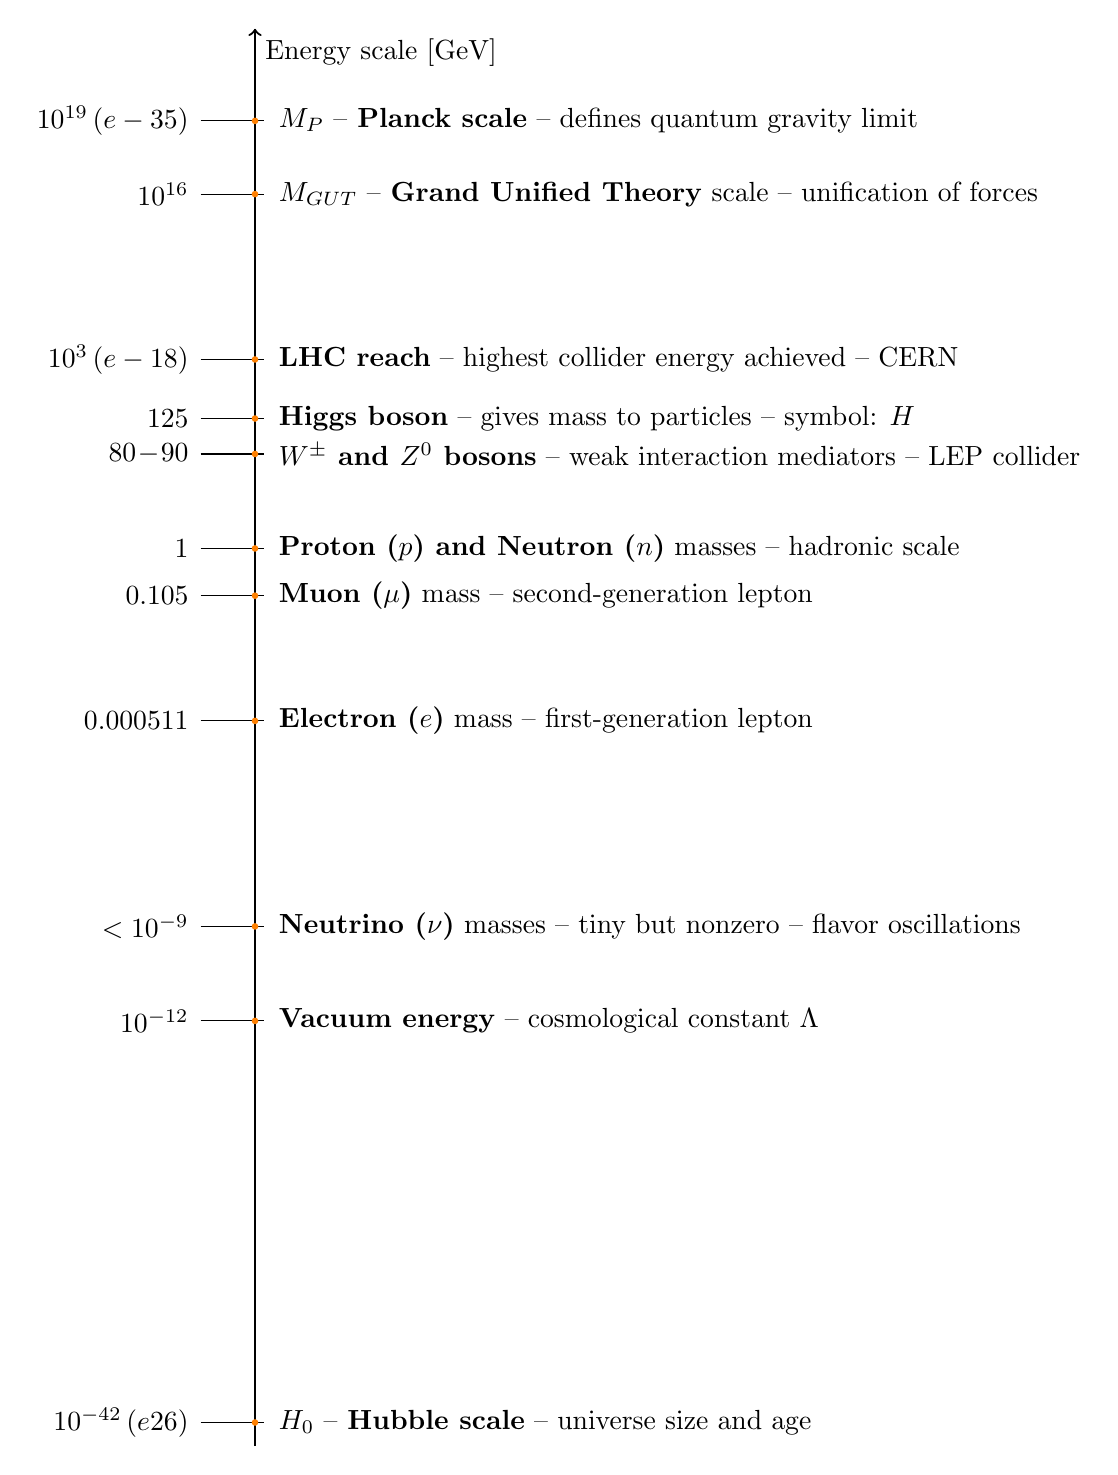
\begin{tikzpicture}[scale = .6]

  \draw[thick,->] (0,0) -- (0,30) node[anchor=north west]{Energy scale [GeV]};

  \foreach \y/\E/\desc in {
    16.1/{$10^{19} \, (\SI{e-35}{\meter})$}/ $M_P$ -- \textbf{Planck scale} -- defines quantum gravity limit,
    13/{$10^{16}$}/$M_{\text{GUT}}$ -- \textbf{Grand Unified Theory} scale -- unification of forces,
    6/{$10^3 \, (\SI{e-18}{\meter})$}/\textbf{LHC reach} -- highest collider energy achieved -- CERN,
    3.5/{$125$}/\textbf{Higgs boson} -- gives mass to particles -- symbol: $H$,
    2/{$80\!-\!90$}/\textbf{$W^\pm$ and $Z^0$ bosons} -- weak interaction mediators -- LEP collider,
    -2/{$1$}/\textbf{Proton ($p$) and Neutron ($n$)} masses -- hadronic scale,
    -4/{$0.105$}/\textbf{Muon ($\mu$)} mass -- second-generation lepton,
    -9.3/{$0.000511$}/\textbf{Electron ($e$)} mass -- first-generation lepton,
    -18/{$<10^{-9}$}/\textbf{Neutrino ($\nu$)} masses -- tiny but nonzero -- flavor oscillations,
    -22/{$10^{-12}$}/\textbf{Vacuum energy} -- cosmological constant $\Lambda$,
    -39/{$10^{-42} \, (\SI{e26}{\meter})$}/$H_0$ -- \textbf{Hubble scale} -- universe size and age
  }{
    \pgfmathsetmacro{\yy}{(\y + 40) * 0.5}
    \draw (-1.15,\yy) -- (0.2,\yy);
    \fill[orange] (0,\yy) circle (2pt);
    \node[anchor=east] at (-1.2,\yy) {\E};
    \node[anchor=west,align=justify] at (0.3,\yy) {\desc};
  }

\end{tikzpicture}
\end{figure}

\section{Mechanical Model of a Quantum Field}
\section{Mechanical Model of a Quantum Field}

To build intuition for quantum fields, it is useful to begin with a simple mechanical system: a chain of coupled elastic strings. This model arises as the \textit{continuum limit} of a one-dimensional lattice of \(N\) atoms, and already captures many of the essential features of field theories.

We consider a \textbf{meta-stable} system, meaning that its configuration does not change drastically under the action of a small perturbing force.\footnote{In fact, every physical system is meta-stable in this sense: if a small perturbation could radically alter its configuration, it could not persist in a stable state.} Thus, there must exist a restoring force that drives the system back toward equilibrium.

For a small displacement \(y\) from equilibrium, the restoring force can be expanded in a Taylor series:
\[
    F(y) = F(0) + \left.\frac{dF}{dy}\right|_{y=0} y + \dots
    = -|\kappa|\, y + \mathcal{O}(y^2),
\]
where we set \(F(0) = 0\) (no force at equilibrium) and require \(\left.\tfrac{dF}{dy}\right|_{y=0} = -|\kappa| < 0\) (restoring behavior). The linear term dominates for sufficiently small displacements, showing that any meta-stable system can be modeled, to first approximation, as a collection of coupled harmonic oscillators.

The simplest realization is a chain of \(N\) identical atoms, each of mass \(m\), connected by springs with spring constant \(\kappa\) and arranged along a line with equilibrium spacing \(\Delta\). The total length of the chain is
\[
    L = N \Delta.
\]
The displacement of the \(i\)-th atom from its equilibrium position will be denoted by \(y_i(t)\). For simplicity, we restrict ourselves to transverse displacements along the \(y\)-axis, keeping the equilibrium positions along the \(x\)-axis fixed.

\begin{figure}[H]
    \begin{minipage}{0.45\textwidth}
        \centering
        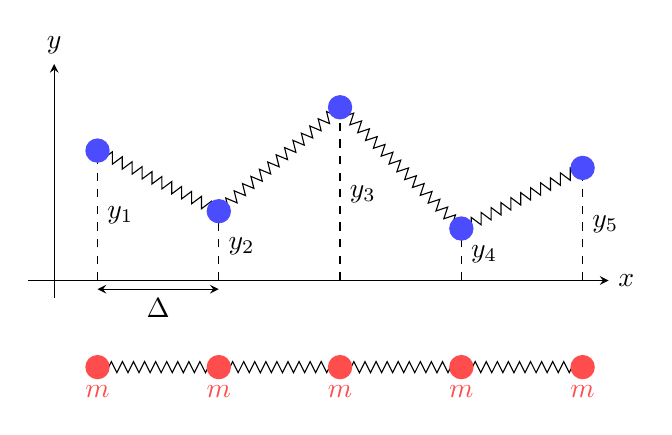
\begin{tikzpicture}[scale=1.1,>=stealth]

            % Horizontal spacing between masses
            \def\Deltax{1.4}

            % Random vertical positions (displacements)
            \def\yA{0.5}
            \def\yB{-0.2}
            \def\yC{1.0}
            \def\yD{-0.4}
            \def\yE{0.3}

            % Reference axes
            \draw[->] (-0.5,-1.2) -- (-0.5,1.5) node[anchor=south]{$y$};
            \draw[->] (-0.8,-1.0) -- (5*\Deltax-1.1,-1.0) node[anchor=west]{$x$};

            % --- Upper part: masses at different y ---
            % Mass vertical positions
            \coordinate (m1) at (0,\yA);
            \coordinate (m2) at (\Deltax,\yB);
            \coordinate (m3) at (2*\Deltax,\yC);
            \coordinate (m4) at (3*\Deltax,\yD);
            \coordinate (m5) at (4*\Deltax,\yE);

            % Springs (zigzag lines)
            \draw[decorate,decoration={zigzag,segment length=4pt,amplitude=2pt}] (m1) -- (m2);
            \draw[decorate,decoration={zigzag,segment length=4pt,amplitude=2pt}] (m2) -- (m3);
            \draw[decorate,decoration={zigzag,segment length=4pt,amplitude=2pt}] (m3) -- (m4);
            \draw[decorate,decoration={zigzag,segment length=4pt,amplitude=2pt}] (m4) -- (m5);

            % Segments and spacings
            \foreach \i/\y in {1/\yA, 2/\yB, 3/\yC, 4/\yD, 5/\yE} {
                    \draw[dashed] (\i*\Deltax-\Deltax,-1) -- (\i*\Deltax-\Deltax,\y) node[midway,right] {$y_{\i}$};
                }
            \draw[<->] (0,-1.1) -- (\Deltax,-1.1) node[midway,below] {$\Delta$};

            % Masses (blue circles)
            \foreach \m in {m1,m2,m3,m4,m5}{
                    \fill[blue!70] (\m) circle (4pt);
                }

            % --- Lower part: horizontal chain ---
            \begin{scope}[yshift=-2cm]
                % Horizontal positions
                \coordinate (n1) at (0,0);
                \coordinate (n2) at (\Deltax,0);
                \coordinate (n3) at (2*\Deltax,0);
                \coordinate (n4) at (3*\Deltax,0);
                \coordinate (n5) at (4*\Deltax,0);

                % Springs
                \draw[decorate,decoration={zigzag,segment length=4pt,amplitude=2pt}] (n1) -- (n2);
                \draw[decorate,decoration={zigzag,segment length=4pt,amplitude=2pt}] (n2) -- (n3);
                \draw[decorate,decoration={zigzag,segment length=4pt,amplitude=2pt}] (n3) -- (n4);
                \draw[decorate,decoration={zigzag,segment length=4pt,amplitude=2pt}] (n4) -- (n5);

                % Masses (red circles)
                \foreach \n in {n1,n2,n3,n4,n5}{
                        \fill[red!70] (\n) circle (4pt);
                        \node[red!70,below=3pt] at (\n) {$m$};
                    }
            \end{scope}

        \end{tikzpicture}
    \end{minipage}
    \hfill
    \begin{minipage}{0.45\textwidth}
        \(y_i=0\) is the equilibrium position of the \(i\)-th atom. The springs exert restoring forces proportional to the relative displacements of neighboring atoms: each atom is under the influence of the neighboring springs, describing a local interaction.

        \(y_i\neq0\) describes the small oscillations around the equilibrium position: transverse \textbf{excitations} of the lattice.
    \end{minipage}
\end{figure}

In the limit \(N\to\infty\) and \(\Delta \to 0\) with \(L\) fixed, the discrete index \(i\) becomes a continuous spatial coordinate and the displacements \(y_i(t)\) become a continuous field \(\phi(x,t)\). This \textbf{continuum limit} transforms the system of coupled oscillators into a continuous field, allowing us to understand the dynamics of fields in terms of familiar mechanical concepts.

\subsection{Discrete case}

To study the dynamics of the chain we employ the Euler--Lagrange equations.
The Lagrangian of the system is constructed as the difference between the kinetic and potential energy contributions of each atom:
\[
    \begin{aligned}
        L & = \sum_{j=1}^N \left[ \frac{1}{2} m \dot{y}_j^2 - \frac{1}{2} k \left(y_j - y_{j+1}\right)^2 \right]                      \\
          & = \sum_{j=1}^N \left[ \frac{1}{2} m \dot{y}_j^2 - \frac{1}{2} \kappa \left(\frac{y_j - y_{j+1}}{\Delta}\right)^2 \right],
    \end{aligned}
\]
where we impose periodic boundary conditions \(j \to j+N\)\footnote{In other words, the first and the last atoms in the chain interact with each other.} and we renamed the spring constant \(k\) as \(\kappa = k \Delta^2\), which is now more of a \textit{coupling constant} between neighboring atoms.

We are assuming small oscillations around the equilibrium configuration, such that the relative displacement between neighboring atoms is small compared to the natural lattice spacing \(\Delta\):
\[
    \frac{y_j - y_{j+1}}{\Delta} \ll 1.
\]

It is worth noting that the coupling constant \(\kappa\) has the dimension of an energy, and can be written as
\[
    \kappa = m v^2,
\]
where \(v\) is a characteristic velocity associated with the propagation of disturbances along the chain. With this identification, the Lagrangian becomes
\[
    L = \frac{1}{2}m \sum_{j=1}^{N} \left[ \dot{y}_j^2(t)
        - v^2\left(\frac{y_j - y_{j+1}}{\Delta}\right)^2  \right],
\]
where the first term corresponds to the kinetic energy of the atoms, while the second encodes the elastic potential energy due to the coupling between neighbors.

The time evolution of the system is obtained by applying the principle of least action:
the motion is such that the variation of the action vanishes,
\[
    S = \int L \, \mathrm{d}t, \qquad \delta S = 0,
\]
which leads to the Euler--Lagrange equations governing the dynamics of the chain.
Recalling the general form
\[
    \frac{\mathrm{d}}{\mathrm{d} t} \frac{\partial L}{\partial \dot{y}_j}
    = \frac{\partial L}{\partial {y}_j},
    \qquad j = 1, \dots , N,
\]
we obtain the governing equations of motion:
\[
    \ddot{y}_j (t)
    = -\,v^2 \left(\frac{2y_j - y_{j+1} - y_{j-1}}{\Delta^2}\right).
\]
This result clearly describes a system of coupled harmonic oscillators: the displacement of the \(j\)-th atom is influenced not only by its own position but also by the relative positions of its nearest neighbors, \((j+1)\) and \((j-1)\).
In other words, each atom is bound to oscillate around equilibrium under the restoring force arising from the springs that connect it to its neighbors.

Solving such a system directly is not convenient, since the equations are not independent. However, there is a natural way to simplify the problem by exploiting the translational symmetry of the lattice. The key idea is to perform a \textit{discrete Fourier transform} of the displacements, which allows us to rewrite the dynamics in terms of normal modes of oscillation. Since \(y_j(t)\) has to be periodic (\(y_j(t) = y_{j+N}(t)\)), we can write:
\[
    y_j(t) = \frac{1}{\sqrt{N}} \sum_{\sigma=1}^{N} e^{i\frac{2\pi}{N}\sigma j} \tilde{y}_{\sigma}(t).
\]
In this new representation, each mode corresponds to a collective oscillation of the entire chain with a definite wavelength. From a mathematical perspective, this amounts to diagonalizing the interaction matrix: the coupling between neighbors is replaced by a set of independent equations for the Fourier modes. In physical terms, the Fourier transform identifies the proper "coordinates" in which the energy of the system can be expressed as a sum of independent contributions, one for each mode.\footnote{In other words, instead of tracking the motion of individual atoms, which are strongly coupled, we describe the system in terms of delocalized excitations (the normal modes), each evolving independently. This step paves the way to the field interpretation: in the continuum limit, these modes will be interpreted as excitations of a quantum field.}

Now, by substituting in the equation of motion, we can decouple the system:
\[
    \begin{aligned}
        \frac{1}{\sqrt{N}} \sum_{\sigma=1}^{N} e^{i\frac{2\pi}{N}\sigma j} \ddot{\tilde{y}}_{\sigma} & = \frac{-1}{\sqrt{N}} \left(\frac{v}{\Delta}\right)^2 \left[ 2 \sum_{\sigma=1}^{N} e^{i\frac{2\pi}{N}\sigma j} \tilde{y}_{\sigma} - \sum_{\sigma=1}^{N} e^{i\frac{2\pi}{N}\sigma (j-1)} \tilde{y}_{\sigma} - \sum_{\sigma=1}^{N} e^{i\frac{2\pi}{N}\sigma (j+1)} \tilde{y}_{\sigma}\right] \\
                                                                                                     & = \frac{-1}{\sqrt{N}} \left(\frac{v}{\Delta}\right)^2 \sum_{\sigma=1}^{N} e^{i\frac{2\pi}{N}\sigma j} \tilde{y}_{\sigma} \left[ 2 - e^{-i\frac{2\pi}{N}\sigma} - e^{i\frac{2\pi}{N}\sigma}\right]                                                                                          \\
                                                                                                     & = \frac{-1}{\sqrt{N}} \left(\frac{v}{\Delta}\right)^2 \sum_{\sigma=1}^{N} e^{i\frac{2\pi}{N}\sigma j} \tilde{y}_{\sigma} \left[ 2 - 2 \cos(\frac{2\pi}{N}\sigma)\right]                                                                                                                    \\
        \iff \ddot{\tilde{y}}_{\sigma}(t)                                                            & = - 2 \frac{v^2}{\Delta^2} \left[ 1 - \cos(\frac{2\pi}{N}\sigma)\right] \tilde{y}_{\sigma}(t) = - \left( \frac{2v}{\Delta} \sin(\frac{\pi\sigma}{N}) \right)^2 \tilde{y}_{\sigma}(t),
    \end{aligned}
\]
where we have made use of the trigonometric identity
\((1 - \cos(2\theta)) = 2\sin^2(\theta)\). This leads to the following set of equations for the Fourier modes:
\[
    \begin{aligned}
        \ddot{\tilde{y}}_{\sigma}(t) & = - \omega^2_{\sigma}\, \tilde{y}_{\sigma}(t),
        \quad                        &                                                                & \forall \, \sigma = 1,2,\dots,N, \\
        \omega_{\sigma}              & = \frac{2v}{\Delta} \, \sin\!\left(\frac{\pi\sigma}{N}\right).
    \end{aligned}
\]
%
Each Fourier component \(\tilde{y}_{\sigma}(t)\) evolves independently and satisfies the equation of a simple harmonic oscillator with characteristic frequency \(\omega_{\sigma}\).
In other words, the original coupled system of atoms has been diagonalized into a set of \(N\) decoupled oscillators, each associated with a normal mode of vibration.

The general solution for each mode is therefore given by a linear combination of oscillatory functions:
\[
    \tilde{y}_{\sigma}(t)
    = A_{\sigma} e^{-i \omega_{\sigma} t} + B_{\sigma} e^{+i \omega_{\sigma} t},
\]
where the constants \(A_{\sigma}\) and \(B_{\sigma}\) are determined by the initial conditions.
Physically, these modes correspond to standing waves propagating through the chain, each characterized by a discrete wave number and its corresponding frequency.

In practice, we will keep only the negative exponential,
\[
    \tilde{y}_{\sigma}(t) = A_{\sigma} e^{-i \omega_{\sigma} t},
\]
since the positive-frequency solution is automatically recovered as the complex conjugate.
This choice avoids redundancy and is particularly convenient when later quantizing the system, because creation and annihilation operators will naturally emerge from the decomposition into \(e^{-i\omega t}\) and its conjugate.

Now we can plug the solution for the Fourier modes back into the inverse transform in order to recover the displacement of the \(j\)-th atom:
\[
    \begin{aligned}
        y_j(t) & = \frac{1}{\sqrt{N}} \sum_{\sigma=1}^{N} e^{i\frac{2\pi}{N}\sigma j} \tilde{y}_{\sigma}(t)                                                   \\
               & = \frac{1}{\sqrt{N}} \sum_{\sigma=1}^{N} A_{\sigma} e^{i \left( \frac{2\pi}{N}\sigma j - \omega_{\sigma} t \right)}                          \\
               & = \frac{1}{\sqrt{N}} \sum_{\sigma=1}^{N} A_{\sigma} e^{i \left( \frac{2\pi}{N}\frac{\sigma}{\Delta} (\Delta j) - \omega_{\sigma} t \right)},
    \end{aligned}
\]
Here we have reintroduced the lattice spacing \(\Delta\), so that the quantity \(\Delta j\) corresponds exactly to the physical position \(x\) of the \(j\)-th atom along the chain.

This expression shows that the displacement of each atom can be written as a linear superposition of plane waves (like \textit{sound waves}). In particular, the system supports \(N\) different wave numbers, each corresponding to one Fourier mode:
\[
    \kappa_{\sigma} = \frac{2\pi}{N} \frac{\sigma}{\Delta} = \frac{2\pi}{\lambda_{\sigma}}, \qquad \sigma = 1,2,\dots,N,
\]
with associated discrete wavelengths
\[
    \lambda_{\sigma} = \frac{N\Delta}{\sigma} = N\Delta, \, \frac{N\Delta}{2}, \dots, \Delta.
\]

\begin{remark}
    The propagation speed of each mode is obtained as the ratio between its frequency and its wave number:
    \[
        v_{\sigma} = \frac{\omega_{\sigma}}{\kappa_{\sigma}}
        = \frac{\tfrac{2v}{\Delta}\,\sin\!\left(\tfrac{\pi\sigma}{N}\right)}{\tfrac{2\pi}{N}\tfrac{\sigma}{\Delta}}
        = v \,\frac{N}{\pi\sigma} \,\sin\!\left(\tfrac{\pi\sigma}{N}\right).
    \]
    Introducing the parameter \(\theta_{\sigma} = \tfrac{\pi\sigma}{N}\), this can be written in the compact form
    \[
        v_{\sigma} = v\,\frac{\sin(\theta_{\sigma})}{\theta_{\sigma}}.
    \]
    This result shows that each Fourier mode propagates with a distinct phase velocity, depending on the ratio \(\sigma/N\).
    In the continuum limit \(N \to \infty\) with \(\sigma/N \to 0\), one has \(\theta_{\sigma} \to 0\) and therefore
    \[
        \lim_{\theta_{\sigma}\to 0} \frac{\sin(\theta_{\sigma})}{\theta_{\sigma}} = 1,
    \]
    so all modes propagate with the same velocity \(v_{\sigma} \sim v\). This recovers the expected propagation speed of sound waves in the continuous chain.
\end{remark}

\begin{remark}
    The actual number of independent vibrational degrees of freedom is \(N-1\), since the \(N\)-th mode corresponds to a zero frequency:
    \[
        \omega_{\sigma=N} = \frac{2v}{\Delta}\,\sin\!\left(\pi \frac{N}{N}\right) = 0.
    \]
    This means that \(\tilde{y}_N(t)\) does not oscillate in time. Physically, this mode represents a uniform translation of the entire chain, where all atoms are displaced by the same amount. As such, it does not contribute to the internal vibrational dynamics, and the only genuine oscillatory modes are the first \(N-1\).
\end{remark}

\begin{figure}[H]
    \begin{minipage}{0.5\textwidth}
        Moreover we can show that the waves with \(\sigma = s\) and \(\sigma = N-s\) in general have the same frequency \(\omega_s\), since:
        \[
            \begin{aligned}
                \omega_{N-s} & = \frac{2v}{\Delta}\,\sin\!\left(\pi \frac{N-s}{N}\right)           \\
                             & = \frac{2v}{\Delta}\,\sin\!\left(\pi -\frac{\pi s}{N}\right)        \\
                             & = \frac{2v}{\Delta}\,\sin\!\left(\frac{\pi s}{N}\right) = \omega_s.
            \end{aligned}
        \]
    \end{minipage}
    \hfill
    \begin{minipage}{0.45\textwidth}
        \centering
        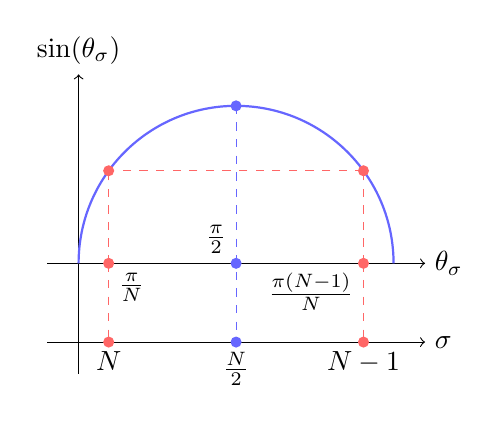
\begin{tikzpicture}[scale=2]
            \draw[->] (-0.2,0) -- (2.2,0) node[right] {$\theta_{\sigma}$};
            \draw[->] (-0.2,-0.5) -- (2.2,-0.5) node[right] {$\sigma$};
            \draw[->] (0,-0.7) -- (0,1.2) node[above] {$\sin(\theta_{\sigma})$};

            \draw[thick, blue!60] (0,0) arc[start angle=180,end angle=0,radius=1];

            \def\N{5}
            \def\xone{pi/\N}
            \def\xtwo{pi*(\N-1)/\N}

            \coordinate (A) at ({1+cos(180*\xone/pi)},{sin(180*\xone/pi)});
            \coordinate (B) at ({1+cos(180*\xtwo/pi)},{sin(180*\xtwo/pi)});
            \coordinate (-A) at ({1+cos(180*\xone/pi)},-0.5);
            \coordinate (-B) at ({1+cos(180*\xtwo/pi)},-0.5);

            \draw[dashed, red!60] (A|-0,0) -- (A);
            \draw[dashed, red!60] (B|-0,0) -- (B);
            \draw[dashed, red!60] (A|-0,0) -- (-A);
            \draw[dashed, red!60] (B|-0,0) -- (-B);
            \draw[dashed, red!60] (A) -- (B);
            \draw[dashed, blue!60] (1,1) -- (1,-0.5);

            \node[below left] at (A|-0,0) {$\frac{\pi(N-1)}{N}$};
            \node[below right] at (B|-0,0) {$\frac{\pi}{N}$};
            \node[below] at (A|-0,-0.5) {$N-1$};
            \node[below] at (B|-0,-0.5) {$N$};
            \node[above left] at (1,0) {$\frac{\pi}{2}$};
            \node[below] at (1,-0.5) {$\frac{N}{2}$};

            \fill[red!60] (A) circle (1pt);
            \fill[red!60] (B) circle (1pt);
            \fill[red!60] (A|-0,0) circle (1pt);
            \fill[red!60] (B|-0,0) circle (1pt);
            \fill[red!60] (A|-0,-0.5) circle (1pt);
            \fill[red!60] (B|-0,-0.5) circle (1pt);
            \fill[blue!60] (1,0) circle (1pt);
            \fill[blue!60] (1,1) circle (1pt);
            \fill[blue!60] (1,-0.5) circle (1pt);
        \end{tikzpicture}
    \end{minipage}
\end{figure}

We can interpret the two modes with the same frequency as forming a single complex degree of freedom. This interpretation is supported by the observation that the original variable \(y_j\) is real, even though it is expressed as a sum of complex exponentials:
\[
    \begin{aligned}
        y_j(t)   & = \frac{1}{\sqrt{N}} \sum_{\sigma=1}^{N} e^{i\frac{2\pi}{N}\sigma j} \tilde{y}_{\sigma}(t),    \\
        y_j^*(t) & = \frac{1}{\sqrt{N}} \sum_{\sigma=1}^{N} e^{-i\frac{2\pi}{N}\sigma j} \tilde{y}_{\sigma}^*(t). \\
    \end{aligned}
\]
Thus, by requiring that the two expressions coincide, we can compute:
\[
    \begin{aligned}
        \sum_{\sigma=1}^{N} e^{i\frac{2\pi}{N}\sigma j} \tilde{y}_{\sigma}(t)                  & = \sum_{\sigma=1}^{N} e^{-i\frac{2\pi}{N}\sigma j} \tilde{y}_{\sigma}^*(t), \\
        \sum_{\sigma=N-1}^{0} e^{i\frac{2\pi}{N}(N-\sigma) j} \tilde{y}_{N-\sigma}(t)          & = \sum_{\sigma=1}^{N} e^{-i\frac{2\pi}{N}\sigma j} \tilde{y}_{\sigma}^*(t), \\
        \sum_{\sigma=N-1}^{0} e^{i2\pi j} e^{-i\frac{2\pi}{N}\sigma j} \tilde{y}_{N-\sigma}(t) & = \sum_{\sigma=1}^{N} e^{-i\frac{2\pi}{N}\sigma j} \tilde{y}_{\sigma}^*(t), \\
        \sum_{\sigma=N-1}^{0} e^{-i\frac{2\pi}{N}\sigma j} \tilde{y}_{N-\sigma}(t)             & = \sum_{\sigma=1}^{N} e^{-i\frac{2\pi}{N}\sigma j} \tilde{y}_{\sigma}^*(t), \\
        \sum_{\sigma=1}^{N} e^{-i\frac{2\pi}{N}\sigma j} \tilde{y}_{N-\sigma}(t)               & = \sum_{\sigma=1}^{N} e^{-i\frac{2\pi}{N}\sigma j} \tilde{y}_{\sigma}^*(t), \\
        \sum_{\sigma=1}^{N} \left[ \tilde{y}_{N-\sigma}(t) - \tilde{y}_{\sigma}^*(t) \right]   & = 0,
    \end{aligned}
\]
which lead us to conclude that \(\tilde{y}_{N-\sigma}(t) = \tilde{y}_{\sigma}^*(t)\).\footnote{In the first step, we rename the summation index on the right-hand side of the equation, replacing each \(\sigma\) with \(N - \sigma\). We then use the periodicity condition \(e^{i 2\pi j} = 1\) to simplify the exponential factor. Next, we reverse the order of summation and, since the terms corresponding to \(\sigma = 0\) and \(\sigma = N\) are identical, we can safely rewrite the sum over the range \(1 \leq \sigma \leq N\).}

Now we are in a position to compute the total number of independent vibrational degrees of freedom. To do so, we must distinguish two cases:
\begin{itemize}
    \item \textbf{If \(N\) is even (\(N = 2l\))}, the total number of pairs of harmonic oscillators with the same frequency (denoted by \(m\)) is
          \[
              m = \frac{2l - 2}{2} = l - 1 .
          \]
          In this case we have to exclude the modes \(\sigma = N\) and \(\sigma = \frac{N}{2}\). The reason is that, when \(N\) is even, the mode with index \(\sigma = \frac{N}{2}\) is self-conjugate, since it coincides with its complementary mode \(\sigma = N - \frac{N}{2} = \frac{N}{2}\).

    \item \textbf{If \(N\) is odd (\(N = 2l+1\))}, the total number of such oscillator pairs is
          \[
              m = \frac{(2l+1) - 1}{2} = l .
          \]
          Here the only index that must be removed is \(\sigma = N\), since \(\frac{N}{2}\) is not an integer and therefore does not correspond to any mode index.
\end{itemize}
The two oscillators associated with the same frequency can be regarded as components of a single complex degree of freedom. In this representation, the physical displacement corresponds to the real part of the complex variable, while the imaginary part encodes the redundant conjugate mode.

We can now exploit the solutions obtained in the new basis to diagonalize the Hamiltonian, since the transformation allows us to rewrite it in terms of independent normal modes, each of which behaves as an uncoupled harmonic oscillator. Let us temporarily neglect the contributions from the modes $\sigma = \frac{N}{2}, N$. Then the kinetic energy can be rewritten as
\[
    \begin{aligned}
        T & = \frac{1}{2}m \sum_{j=1}^N \dot{y}_j^2                                                                                                                                                                                                                                                                                                                                       \\
          & = \frac{1}{2}m \sum_{j=1}^N \frac{1}{N} \sum_{\sigma=1}^{\frac{N}{2}-1} \left( e^{i \frac{2\pi}{N}\sigma j} \dot{\tilde{y}}_{\sigma} + e^{-i \frac{2\pi}{N}\sigma j} \dot{\tilde{y}}_{N-\sigma} \right) \sum_{\xi=1}^{\frac{N}{2}-1} \left( e^{i \frac{2\pi}{N}\xi j} \dot{\tilde{y}}_{\xi} + e^{-i \frac{2\pi}{N}\xi j} \dot{\tilde{y}}_{N-\xi} \right)                      \\
          & = \frac{1}{2}m \sum_{\sigma,\xi=1}^{\frac{N}{2}-1} \left[ \dot{\tilde{y}}_{\sigma} \dot{\tilde{y}}_{\xi} \left( \frac{1}{N} \sum_{j=1}^N e^{i \frac{2\pi}{N}(\sigma+\xi) j} \right) + \dot{\tilde{y}}_{N-\sigma} \dot{\tilde{y}}_{\xi} \left( \frac{1}{N} \sum_{j=1}^N e^{i \frac{2\pi}{N}(\xi-\sigma) j} \right) \right.                                                     \\
          & \qquad\qquad\qquad+ \left. \dot{\tilde{y}}_{\sigma} \dot{\tilde{y}}_{N-\xi} \left( \frac{1}{N} \sum_{j=1}^N e^{i \frac{2\pi}{N}(\sigma-\xi) j} \right) + \dot{\tilde{y}}_{N-\sigma} \dot{\tilde{y}}_{N-\xi} \left( \frac{1}{N} \sum_{j=1}^N e^{-i \frac{2\pi}{N}(\sigma+\xi) j} \right) \right]                                                                               \\
          & = \frac{1}{2}m \sum_{\sigma,\xi=1}^{\frac{N}{2}-1} \left( \dot{\tilde{y}}_{\sigma} \dot{\tilde{y}}_{\xi} \, \delta_{\sigma+\xi, 0} + \dot{\tilde{y}}_{N-\sigma} \dot{\tilde{y}}_{\xi} \, \delta_{\sigma,\xi} + \dot{\tilde{y}}_{\sigma} \dot{\tilde{y}}_{N-\xi} \, \delta_{\sigma,\xi} + \dot{\tilde{y}}_{N-\sigma} \dot{\tilde{y}}_{N-\xi} \, \delta_{\sigma+\xi, 0} \right) \\
          & = \frac{1}{2}m \sum_{\sigma=1}^{\frac{N}{2}-1} \left( 2 \dot{\tilde{y}}_{\sigma} \dot{\tilde{y}}_{N-\sigma} \right) = m \sum_{\sigma=1}^{\frac{N}{2}-1} \dot{\tilde{y}}_{\sigma} \dot{\tilde{y}}_{\sigma}^* = m \sum_{\sigma=1}^{\frac{N}{2}-1} \vert \dot{\tilde{y}}_{\sigma} \vert ^2.
    \end{aligned}
\]
The sum over $j$ enforce orthogonality, which manifests as Kronecker deltas. These deltas select only the diagonal terms, pairing each mode $\sigma$ with its complex conjugate $N-\sigma$. The final expression is a sum over independent Fourier modes, where the kinetic energy is simply the mass times the squared modulus of the time derivative of each mode amplitude. Now for the potential energy:
\[
    \begin{aligned}
        V & = \frac{1}{2} m \left( \frac{v}{\Delta} \right)^2 \sum_{j=1}^N \left( y_j - y_{j+1} \right)^2 =                                                                                                                                                                                                               \\
          & = \frac{1}{2} m \left( \frac{v}{\Delta} \right)^2 \sum_{j=1}^N \left[\sum_{\sigma=1}^{\frac{N}{2}-1} \left[ \left( e^{i \frac{2\pi}{N}\sigma j} \tilde{y}_{\sigma} + e^{-i \frac{2\pi}{N}\sigma j} \tilde{y}_{N-\sigma} \right) \right.\right.                                                                \\
          & \qquad\qquad\qquad\qquad \left.\left.- \left( e^{i \frac{2\pi}{N}\sigma (j+1)} \tilde{y}_{\sigma} + e^{-i \frac{2\pi}{N}\sigma (j+1)} \tilde{y}_{N-\sigma} \right) \right] \right]^2                                                                                                                          \\
          & = \frac{1}{2} m \left( \frac{v}{\Delta} \right)^2 \sum_{j=1}^N \left[\sum_{\sigma=1}^{\frac{N}{2}-1} \left[ \tilde{y}_{\sigma} e^{i \alpha_{\sigma}  j} \left( 1 - e^{i \alpha_{\sigma}} \right) + \tilde{y}_{N-\sigma} e^{-i \alpha_{\sigma}  j} \left( 1 - e^{-i \alpha_{\sigma}} \right) \right] \right]^2 \\
          & = \frac{1}{2} m \left( \frac{v}{\Delta} \right)^2 \sum_{j=1}^N \left[\sum_{\sigma=1}^{\frac{N}{2}-1} 2i \sin(\frac{\alpha_{\sigma}}{2}) \left( - \tilde{y}_{\sigma} e^{i \alpha_{\sigma} (j+\tfrac12)} + \tilde{y}_{N-\sigma} e^{-i \alpha_{\sigma} (j+\tfrac12)} \right) \right]^2,
    \end{aligned}
\]
where \(\alpha_{\sigma} = \frac{2\pi}{N}\sigma\). Now, using again the sum over \(j\) to enforce orthogonality (noting that the term \(j+\tfrac12\) on the exponential does not influence the result since it is canceled in cross-terms, while diagonal terms are zeroed by \(\delta_{\sigma+\xi,0}\)) and recalling the expression for \(\omega_{\sigma}\), we arrive to the diagonal form of the potential:
\[
    V = \frac{1}{2} m \left( \frac{v}{\Delta} \right)^2 \sum_{\sigma=1}^{\frac{N}{2}-1} 8 \sin(\frac{\alpha_{\sigma}}{2})^2 \tilde{y}_{\sigma}\tilde{y}_{N-\sigma} = m \sum_{\sigma=1}^{\frac{N}{2}-1} \omega_{\sigma}^2 \vert \tilde{y}_{\sigma} \vert^2.
\]
Finally, by adding the contributions from the modes $\sigma = \frac{N}{2}, N$, we arrive to the diagonal form of our Lagrangian:
\[
    L = m \sum_{\sigma=1}^{\frac{N}{2}-1} \left( \vert \dot{\tilde{y}}_{\sigma} \vert ^2 - \omega_{\sigma}^2 \vert \tilde{y}_{\sigma} \vert^2 \right) + \frac{m}{2} \left( \dot{\tilde{y}}_{\frac{N}{2}}^2 + \dot{\tilde{y}}_{N}^2 - \omega_{\frac{N}{2}}^2 \tilde{y}_{\frac{N}{2}}^2 \right),
\]
since \(\omega_N = 0\).\footnote{Let us remember that the \(\frac{N}{2}\)-th mode is absent when \(N\) is odd.} Thus, in the end, we have \(\tfrac{N-2}{2}\) complex degrees of freedom from the first term, which become \(N-2\) real degrees of freedom with \(\tfrac{N-2}{2}\) different frequencies, while the second term contributes with 2 real degrees of freedom.

In practice, the diagonalization procedure eliminates the cross-terms that mix different coordinates, leaving a sum of quadratic contributions that can be interpreted as the energies of the individual modes. As a result, the system is reduced to a collection of independent harmonic oscillators, each characterized by its own frequency.

\subsubsection{Quantization}

In order to proceed with the quantization of the system, it is useful to briefly recall the main ingredients of the quantum harmonic oscillator.

We start from the Hamiltonian operator expressed in terms of the position and momentum operators \(\hat y\) and \(\hat p\):
\[
    \hat{H} = \frac{\hat{p}^2}{2m} + \frac{1}{2} m \omega^2 \hat{y}^2 .
\]

The canonical quantization rule imposes the commutation relation between \(\hat y\) and \(\hat p\):
\[
    [\hat{y}, \hat{p}] = i \hbar .
\]
It is then convenient to introduce the so--called ladder (or creation/annihilation) operators:
\[
    \hat{a} = \sqrt{\frac{m\omega}{2\hbar}} \, \hat{y} + \frac{i}{\sqrt{2m\hbar\omega}} \, \hat{p},
    \qquad
    \hat{a}^\dagger = \sqrt{\frac{m\omega}{2\hbar}} \, \hat{y} - \frac{i}{\sqrt{2m\hbar\omega}} \, \hat{p}.
\]
These operators satisfy the commutation relation \( [\hat{a}, \hat{a}^\dagger] = 1 \). In terms of \(\hat{a}\) and \(\hat{a}^\dagger\), the Hamiltonian takes the following simple form:
\[
    \hat{H} = \hbar \omega \left(\hat{a}^\dagger \hat{a} + \tfrac{1}{2}\right).
\]
Finally, the position and momentum operators can be expressed back in terms of the ladder operators as
\[
    \hat{y} = \sqrt{\frac{\hbar}{2m\omega}} \, \big(\hat{a} + \hat{a}^\dagger \big),
    \qquad
    \hat{p} = i \sqrt{\frac{m\hbar\omega}{2}} \, \big(\hat{a}^\dagger - \hat{a}\big).
\]
We now examine the action of the ladder operators by considering their commutators with the Hamiltonian. To understand how the operators affect the energy states, let us compute the commutator with the annihilation operator $\hat a$:
\[
    [\hat H, \hat a] = \hbar \omega \, [\hat a^\dagger \hat a, \hat a].
\]
Using the general identity $[AB,C] = A[B,C] + [A,C]B$, we obtain
\[
    [\hat a^\dagger \hat a, \hat a] = \hat a^\dagger [\hat a,\hat a] + [\hat a^\dagger, \hat a] \hat a = -\hat a,
\]
so that
\[
    [\hat H, \hat a] = - \hbar \omega \, \hat a.
\]
Similarly, for the creation operator $\hat a^\dagger$, we have
\[
    [\hat H, \hat a^\dagger] = \hbar \omega \, [\hat a^\dagger \hat a, \hat a^\dagger] = \hbar \omega \, \hat a^\dagger.
\]

From these commutators, one can immediately deduce the action of the Hamiltonian on the states $\hat a |n\rangle$ and $\hat a^\dagger |n\rangle$. Using $\hat H |n\rangle = \hbar \omega \left(n + \tfrac12\right) |n\rangle$, we find
\[
    \hat H (\hat a |n\rangle) = (\hat a \hat H + [\hat H, \hat a]) |n\rangle = \hbar \omega \left(n - \tfrac12\right) (\hat a |n\rangle),
\]
\[
    \hat H (\hat a^\dagger |n\rangle) = (\hat a^\dagger \hat H + [\hat H, \hat a^\dagger]) |n\rangle = \hbar \omega \left(n + \tfrac32\right) (\hat a^\dagger |n\rangle).
\]
These results show explicitly that $\hat a$ lowers the energy of a state by one quantum $\hbar \omega$, while $\hat a^\dagger$ raises the energy by the same amount.

It is convenient to introduce the number operator, defined as
\[
    \hat N = \hat a^\dagger \hat a.
\]
This operator counts the number of quanta in a given state, since its action on the energy eigenstates is
\[
    \hat N |n\rangle = n |n\rangle.
\]
The ladder operators then have a simple interpretation in terms of the number operator: the annihilation operator $\hat a$ lowers the quantum number by one,
\[
    \hat a |n\rangle = \sqrt{n}\, |n-1\rangle,
\]
while the creation operator $\hat a^\dagger$ raises it by one,
\[
    \hat a^\dagger |n\rangle = \sqrt{n+1}\, |n+1\rangle.
\]
In this way, the states $|n\rangle$ can be constructed by successive application of $\hat a^\dagger$ starting from the vacuum state $|0\rangle$, and the number operator provides a direct measure of the excitation level of each state. These operators are the cornerstone for describing the spectrum and dynamics of the quantum harmonic oscillator.

We are now ready to quantize our \textit{mechanical string} with Lagrangian:
\[
    L = m \sum_{\sigma=1}^{\frac{N}{2}-1} \left( \vert \dot{\tilde{y}}_{\sigma} \vert ^2 + \omega_{\sigma}^2 \vert \tilde{y}_{\sigma} \vert^2 \right) + \frac{m}{2} \left( \dot{\tilde{y}}_{\frac{N}{2}}^2 + \dot{\tilde{y}}_{N}^2 + \omega_{\frac{N}{2}}^2 \tilde{y}_{\frac{N}{2}}^2 \right),
\]
It is useful to stress that each complex mode can be decomposed into its real and imaginary parts. In particular,
\[
    \tilde{y}_{\sigma} = \frac{1}{\sqrt{2}}(\Re \tilde{y}_{\sigma} + \Im \tilde{y}_{\sigma}) = \frac{\tilde{y}_{\sigma}^{(\mathrm{R})}+\tilde{y}_{\sigma}^{(\mathrm{I})}}{\sqrt{2}},
\]
so that the kinetic term can be written as
\[
    \vert \dot{\tilde{y}}_{\sigma} \vert ^2 = \frac{1}{2}\left[ (\dot{\tilde{y}}_{\sigma}^{(\mathrm{R})})^2 + (\dot{\tilde{y}}_{\sigma}^{(\mathrm{I})})^2 \right].
\]
For the real normal modes (e.g. the special indices \(\sigma=\frac{N}{2},N\)) we introduce the usual ladder operators \(\hat a_r,\hat a_r^\dagger\) and have
\[
    \hat{\tilde{y}}_{\sigma}^{(\mathrm{R})} = \sqrt{\frac{\hbar}{2 m \omega_{\sigma}}}\;(\hat a_{\sigma}^{(\mathrm{R})} + \hat a_{\sigma}^{\dagger(\mathrm{R})}),
    \qquad
    \hat{p}_{\sigma}^{(\mathrm{R})} = i\sqrt{\frac{m\hbar\omega_{\sigma}}{2}}\;(\hat a_{\sigma}^{(\mathrm{R})} - \hat a_{\sigma}^{\dagger(\mathrm{R})}),
\]
\[
    \hat{\tilde{y}}_{\sigma}^{(\mathrm{I})} = \sqrt{\frac{\hbar}{2 m \omega_{\sigma}}}\;(\hat a_{\sigma}^{(\mathrm{I})} + \hat a_{\sigma}^{\dagger(\mathrm{I})}),
    \qquad
    \hat{p}_{\sigma}^{(\mathrm{I})} = i\sqrt{\frac{m\hbar\omega_{\sigma}}{2}}\;(\hat a_{\sigma}^{(\mathrm{I})} - \hat a_{\sigma}^{\dagger(\mathrm{I})}),
\]
\[
    \hat{\tilde{y}}_{\frac{N}{2}} = \sqrt{\frac{\hbar}{2 m \omega_{\frac{N}{2}}}}\;(\hat a_{\frac{N}{2}} + \hat a_{\frac{N}{2}}^{\dagger}),
    \qquad
    \hat{p}_{\frac{N}{2}} = i\sqrt{\frac{m\hbar\omega_{\frac{N}{2}}}{2}}\;(\hat a_{\frac{N}{2}} - \hat a_{\frac{N}{2}}^{\dagger}),
\]

The natural framework to describe our quantized mechanical string is the \textbf{Fock space}, which allows us to account for an arbitrary number of excitations in each mode.

Formally, the Fock space is constructed as the direct sum of $n$-particle Hilbert spaces:
\[
    \mathcal{F} = \bigoplus_{n=0}^{\infty} \mathcal{H}^{(n)}
    = \mathcal{H}^{(0)} \oplus \mathcal{H}^{(1)} \oplus \mathcal{H}^{(2)} \oplus \dots,
\]
where $\mathcal{H}^{(0)} \cong \mathbb{C}$ represents the vacuum (the state with no phonons), while for $n \ge 1$ we define
\[
    \mathcal{H}^{(n)} = \underbrace{\mathcal{H}^{(1)} \otimes \mathcal{H}^{(1)} \otimes \dots \otimes \mathcal{H}^{(1)}}_{n \text{ times}}.
\]

Here, $\mathcal{H}^{(1)}$ is the Hilbert space of a single phonon, $\mathcal{H}^{(2)}$ is the space of two phonons, and in general $\mathcal{H}^{(n)}$ describes $n$ phonons. Each $\mathcal{H}^{(n)}$ is a subspace where the total number of excitations is fixed, and the tensor product structure reflects the fact that each phonon can occupy its own independent state within the mode basis.

The Fock space $\mathcal{F}$ as a whole thus contains all possible states with any number of phonons. This construction is crucial because in a quantum harmonic system the number of excitations is not fixed: the system can fluctuate between states with zero, one, or arbitrarily many phonons. Using the Fock space, we can systematically describe the action of creation and annihilation operators, build eigenstates of the total Hamiltonian, and keep track of the occupation numbers of all modes simultaneously.
\begin{itemize}
    \item \(\mathcal{H}^{(1)}\) is spanned by:
          \[
              \hat a_{\sigma}^{\dagger(\mathrm{R})} \ket{0}, \quad \hat a_{\sigma}^{\dagger(\mathrm{I})} \ket{0}, \quad \hat a_{\frac{N}{2}}^{\dagger} \ket{0}, \quad \sigma = 1, \dots, \frac{N}{2}-1,
          \]
          which we can denote more compactly as \(\hat a_{i}^{\dagger} \ket{0}\).
    \item \(\mathcal{H}^{(2)}\) is spanned by all two-phonon states, obtained by applying any two creation operators to the vacuum:
          \[
              \hat a_i^\dagger \hat a_j^\dagger \ket{0}, \qquad i,j = 1,2,\dots, N-1,
          \]
          including the possibility \(i=j\) (two phonons in the same mode).\footnote{One should properly symmetrize the two-phonon states, for instance:  \(\frac{1}{\sqrt{2}} \big( \hat a_i^\dagger \hat a_j^\dagger \ket{0} \pm \hat a_j^\dagger \hat a_i^\dagger \ket{0} \big)\), to ensure the correct bosonic/fermionic symmetry.}

    \item In general, \(\mathcal{H}^{(n)}\) is spanned by all $n$-phonon states:
          \[
              (\hat a_{i_1}^\dagger)^{n_1} (\hat a_{i_2}^\dagger)^{n_2} \dots (\hat a_{i_l}^\dagger)^{n_l} \ket{0}, \qquad \text{with } n_1 + n_2 + \dots + n_l = n,
          \]
          which include all possible distributions of $n$ phonons among the modes. Each \(\mathcal{H}^{(n)}\) is thus the subspace of the Fock space with exactly $n$ excitations.
\end{itemize}
Thus, we can define the vacuum more rigorously as
\[
    \ket{0} = \ket{0}_{\omega_1}^{(\mathrm{R})} \otimes \ket{0}_{\omega_1}^{(\mathrm{I})} \otimes \dots \otimes \ket{0}_{\omega_{N/2-1}}^{(\mathrm{R})} \otimes \ket{0}_{\omega_{N/2-1}}^{(\mathrm{I})} \otimes \ket{0}_{\omega_{N/2}} = \ket{0,0,\dots,0},
\]
so that the action of the creation operators gives
\[
    \hat a_{1}^{\dagger(\mathrm{R})} \ket{0} = \ket{1,0,\dots,0},
    \qquad
    \hat a_{1}^{\dagger(\mathrm{I})} \ket{0} = \ket{0,1,\dots,0},
\]
meaning that we now have a single phonon with frequency \(\omega_1\) in either the real or imaginary part of the mode.

We can now express an arbitrary \textbf{base element} of our Fock space as
\[
    \ket{n_1^{(\mathrm{R})}, \, n_1^{(\mathrm{I})}, \dots, n_{N/2-1}^{(\mathrm{R})}, \, n_{N/2-1}^{(\mathrm{I})}, \, n_{N/2}},
\]
that is, by explicitly specifying the number of phonons in each independent mode of the system. Equivalently, such a state can be written in terms of creation operators as
\[
    C \, \left(\hat a_{1}^{\dagger(\mathrm{R})}\right)^{n_1^{(\mathrm{R})}}
    \left(\hat a_{1}^{\dagger(\mathrm{I})}\right)^{n_1^{(\mathrm{I})}}
    \dots
    \left(\hat a_{N/2}^{\dagger}\right)^{n_{N/2}} \ket{0},
\]
where the constant \(C\) ensures the correct normalization of the state. The integers \(n_i^{(\mathrm{R})}\) and \(n_i^{(\mathrm{I})}\) represent the occupation numbers of the real and imaginary components of the mode with frequency \(\omega_i\), their sum gives the total number of phonons in the mode \(\omega_i\).

Therefore, a \textbf{generic Fock state} encodes the excitation content of the string: although the total number of phonons in the system is finite for each specific state, every mode can host an arbitrarily large number of excitations, which makes the Fock space infinite-dimensional. It can be expressed as:
\[
    \ket{\Psi} = \sum_{n_1^{(\mathrm{R})}}^{\infty}\sum_{n_1^{(\mathrm{I})}}^{\infty} \cdots \sum_{n_{N/2}}^{\infty} C_{n_1^{(\mathrm{R})} n_1^{(\mathrm{I})} \dots n_{N/2}} \ket{n_1^{(\mathrm{R})}, \, n_1^{(\mathrm{I})}, \dots, \, n_{N/2}},
\]
where \(\vert C_{n_1^{(\mathrm{R})} n_1^{(\mathrm{I})} \dots n_{N/2}} \vert^2 \) gives the probability of finding the system in the specific configuration with \(n_1^{(\mathrm{R})} + n_1^{(\mathrm{I})}\) phonons in the first mode and so on, up to \(n_{N/2}\) phonons in the last mode. Clearly, this probabilistic description is valid only if
\[
    \lVert \Psi \rVert^2 = \langle \Psi | \Psi \rangle = \sum_{n_1^{(\mathrm{R})}}^{\infty}\sum_{n_1^{(\mathrm{I})}}^{\infty} \cdots \sum_{n_{N/2}}^{\infty} \vert C_{n_1^{(\mathrm{R})} n_1^{(\mathrm{I})} \dots n_{N/2}} \vert^2 = 1.
\]

Now that we have obtained the explicit form of the energy eigenstates, the last step is to express the Hamiltonian in terms of the ladder operators. In this way, the full quantum description of the system becomes transparent: each mode of the string behaves as an independent quantum harmonic oscillator, whose excitations correspond to phonons.
\[
    \hat{H} = \sum_{\sigma=1}^{\frac{N}{2}-1} \left[ \omega_{\sigma} \left( \hat a_{\sigma}^{\dagger(\mathrm{R})} \hat a_{\sigma}^{(\mathrm{R})} + \hat a_{\sigma}^{\dagger(\mathrm{I})} \hat a_{\sigma}^{(\mathrm{I})} + 1 \right) \right] + \omega_{\frac{N}{2}}\left( \hat a_{\frac{N}{2}}^{\dagger} \hat a_{\frac{N}{2}} + \frac{1}{2} \right),
\]
The Hamiltonian can be rewritten in terms of the number operators, making it clear that the total energy is simply the sum of the contributions of all the phonons. This parallels the case of free particles, where the energy is the sum of the individual excitations:
\[
    \hat{H} = \sum_{\sigma=1}^{\frac{N}{2}-1} \left[ \omega_{\sigma} \left( \hat N_{\sigma}  + 1 \right) \right] + \omega_{\frac{N}{2}}\left( \hat N_{\frac{N}{2}} + \frac{1}{2} \right).
\]
An important feature that emerges is the presence of a non-vanishing vacuum energy: even in the absence of phonons, the ground state carries a finite amount of energy due to the zero-point motion of each mode:
\[
    E_0 = \sum_{\sigma=1}^{\frac{N}{2}-1} \omega_{\sigma} + \frac{\omega_{\frac{N}{2}}}{2}.
\]
This vacuum energy can become very large when summing over all modes, but in a theory without gravity it can be consistently shifted to zero, since only energy differences are physically relevant.

\subsection{Continuum Limit}

We now consider the continuum limit of our discrete system. This is achieved by letting the natural spacing between points on the string, denoted by $\Delta$, tend to zero, while keeping the total length $L$ of the string fixed. To enforce this constraint, we impose the relation $L = N \Delta$ and take the limits $N \to \infty$ and $\Delta \to 0$ simultaneously.

In this limit, the discrete indices $j$ and $\sigma$ transition into continuous variables. As a result, quantities that were previously discrete—such as the wavelength $\lambda_{\sigma}$ and the wave number $\kappa_{\sigma}$—become continuous:
\[
    \begin{aligned}
        \kappa_{\sigma}  & = \frac{2\pi \sigma}{N \Delta} = \frac{2\pi \sigma}{L}, \quad \kappa_{\sigma} \in \left[\frac{2\pi}{L},\, \infty \right), \\
        \lambda_{\sigma} & = \frac{N \Delta}{\sigma} = \frac{L}{\sigma}, \quad \lambda_{\sigma} \in (0,\, L].
    \end{aligned}
\]
As $N \to \infty$ and $\Delta \to 0$, both $\kappa_{\sigma}$ and $\lambda_{\sigma}$ sweep out continuous ranges: $\kappa_{\sigma},\,\lambda_{\sigma} \in [0,\,\infty)$.

Simultaneously, the discrete spatial coordinate becomes a continuous variable. By defining $x = j \Delta$, the displacement variable $y_j$ becomes a smooth field $\psi(x,t)$. Thus, the original system of $N$ coupled harmonic oscillators is reformulated as an infinite set of decoupled harmonic oscillators, each labeled by a continuous wave number $\kappa$:
\[
    \omega_{\sigma} = 2 \frac{v}{\Delta} \sin\left(\frac{\pi \sigma}{N}\right) \xrightarrow[N \to \infty]{} \frac{v}{\Delta} \cdot \frac{2\pi \sigma}{N} = v \kappa_{\sigma}
\]

In this limit, all wave modes propagate with the same velocity:
\[
    v_{\sigma} = \frac{\omega_{\sigma}}{\kappa_{\sigma}} = 2 \frac{v}{\Delta} \sin\left(\frac{\pi \sigma}{N}\right) \cdot \frac{N \Delta}{2\pi \sigma} \xrightarrow[N \to \infty]{} v
\]
This result reflects a key feature of the continuum limit: the dispersion relation becomes linear, and all modes—regardless of their wavelength—travel at the same speed \(v\). This uniform propagation speed is characteristic of non-dispersive media and simplifies the dynamics considerably.

We are thus left with an infinite continuum of independent harmonic oscillators, each labeled by a continuous wave number \(\kappa\) and oscillating with frequency \(\omega_{\kappa} = v \kappa\). Physically, each oscillator corresponds to a traveling wave mode on the string, and the entire system can be viewed as a superposition of such modes, each propagating at speed \(v\).

Upon quantization, these classical vibrational modes become \textit{phonons}—the quantized excitations of the elastic medium. Each phonon carries energy and momentum, and the linear dispersion relation implies that their energy is directly proportional to their momentum.

If we now identify the propagation speed \(v\) with the speed of light \(c\), the dispersion relation takes the form:
\[
    \omega_{\kappa}=c \kappa \iff \hbar \omega_{\kappa}=c \hbar \kappa \implies E = p c,
\]
which is precisely the relativistic energy-momentum relation for a massless particle. This correspondence highlights a deep connection between the quantized excitations of a one-dimensional elastic medium and the behavior of relativistic particles in field theory. In this sense, the phonon becomes a prototype for more general quantum field excitations, including photons and other massless bosons.

\subsubsection{Particle Interpretation}

The field \(\psi(x,t)\) can be interpreted as describing a massless particle in the discrete chain. Upon quantization, excitations at frequency \(\omega_{\kappa}\) of this field — the \textit{phonons} — behave as particles of definite momentum \(\hbar \kappa\) and energy \(\hbar \omega_\kappa\). In this picture, particles of definite momentum emerge as quanta of excitation of the underlying field, created or annihilated by the corresponding creation and annihilation operators. These operators allow us to add or remove a particle of definite momentum from the system state.

\paragraph{Adding a mass term.}
In order to describe a massive particle, we need to introduce a term that tends to restore the system to its equilibrium position. Physically, this can be imagined as an additional spring attached to each atom in the chain, pulling it towards its rest position. This inertial interaction gives rise to a mass term in the continuum limit. Indeed, for a relativistic particle, the energy-momentum relation reads
\[
    E^2 = p^2 c^2 + m^2 c^4,
\]
and the additional spring introduces the \(\kappa_\mu\) term responsible for the \(m^2\) contribution.

\begin{figure}[H]
    \begin{minipage}{0.45\textwidth}
        \centering
        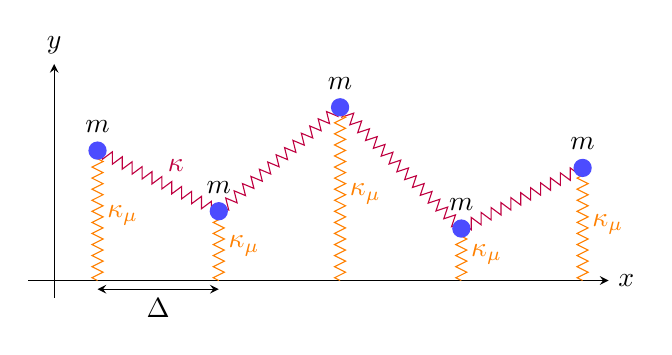
\begin{tikzpicture}[scale=1.1,>=stealth]

            % Horizontal spacing between masses
            \def\Deltax{1.4}

            % Random vertical positions (displacements)
            \def\yA{0.5}
            \def\yB{-0.2}
            \def\yC{1.0}
            \def\yD{-0.4}
            \def\yE{0.3}

            % Reference axes
            \draw[->] (-0.5,-1.2) -- (-0.5,1.5) node[anchor=south]{$y$};
            \draw[->] (-0.8,-1.0) -- (5*\Deltax-1.1,-1.0) node[anchor=west]{$x$};

            % Mass vertical positions
            \coordinate (m1) at (0,\yA);
            \coordinate (m2) at (\Deltax,\yB);
            \coordinate (m3) at (2*\Deltax,\yC);
            \coordinate (m4) at (3*\Deltax,\yD);
            \coordinate (m5) at (4*\Deltax,\yE);

            % Springs (zigzag lines connecting masses)
            \draw[decorate,decoration={zigzag,segment length=4pt,amplitude=2pt}, draw=purple] (m1) -- (m2) node[midway,above right,purple] {$\kappa$};
            \draw[decorate,decoration={zigzag,segment length=4pt,amplitude=2pt}, draw=purple] (m2) -- (m3);
            \draw[decorate,decoration={zigzag,segment length=4pt,amplitude=2pt}, draw=purple] (m3) -- (m4);
            \draw[decorate,decoration={zigzag,segment length=4pt,amplitude=2pt}, draw=purple] (m4) -- (m5);

            % Additional springs for mass term
            \foreach \i/\y in {1/\yA, 2/\yB, 3/\yC, 4/\yD, 5/\yE} {
                    \draw[decorate,decoration={zigzag,segment length=4pt,amplitude=2pt}, draw=orange] (\i*\Deltax-\Deltax,-1) -- (\i*\Deltax-\Deltax,\y) node[midway,right,orange] {$\kappa_{\mu}$};
                }

            % Distance between masses
            \draw[<->] (0,-1.1) -- (\Deltax,-1.1) node[midway,below] {$\Delta$};

            % Masses (blue circles)
            \foreach \m in {m1,m2,m3,m4,m5}{
                    \fill[blue!70] (\m) circle (3pt);
                    \node[above,yshift=3pt] at (\m) {$m$};
                }

        \end{tikzpicture}
    \end{minipage}
    \hfill
    \begin{minipage}{0.45\textwidth}
        The additional elastic constant \(\kappa_\mu\) that tends to restore each particle to its equilibrium position is directly related to the inertial mass of the corresponding particle field.

        For the discrete chain, the Lagrangian can be written as:
    \end{minipage}
\end{figure}
\[
    L = \sum_{j=1}^N \left[ \frac{1}{2} m \dot{y}_j^2  - \frac{1}{2} m v^2 \left( \frac{y_j - y_{j+1}}{\Delta} \right)^2 - \frac{1}{2} \kappa_\mu y_j^2 \right].
\]

Passing to the continuum limit, the discrete sums and differences are replaced by integrals and derivatives:
\[
    \begin{aligned}
        \sum_{j=1}^N                                  & \longrightarrow \int \dd x,                                             \\
        y_j^2                                         & \longrightarrow \psi(x,t)^2,                                            \\
        \dot{y}_j^2                                   & \longrightarrow \left( \frac{\partial \psi(x,t)}{\partial t} \right)^2, \\
        \left( \frac{y_j - y_{j+1}}{\Delta} \right)^2 & \longrightarrow \left( \frac{\partial \psi(x,t)}{\partial x} \right)^2.
    \end{aligned}
\]

Thus, the continuum Lagrangian (with \(v=c=1\)) reads:
\[
    L = \frac{1}{2}m \int \dd x \left[ \left( \frac{\partial \psi(x,t)}{\partial t} \right)^2 - \left( \frac{\partial \psi(x,t)}{\partial x} \right)^2 - \frac{\kappa_\mu}{m} \psi(x,t)^2 \right],
\]
where the last term plays the role of a mass term, proportional to \(m^2\) in natural units. This formulation makes clear how a restoring interaction at the discrete level leads, in the continuum limit, to a massive field with excitations corresponding to massive particles.

Let us now introduce the \textbf{Lagrangian density} \(\mathcal{L}\), which allows us to describe the system in the continuum and relativistic framework. The total Lagrangian is obtained by integrating the Lagrangian density over all space:
\[
    L = \int_{-\infty}^{\infty} \d{x} \mathcal{L}, \quad \text{so that the action reads} \quad S = \int \d{t} L = \int \d{t} \d{x} \mathcal{L}.
\]
Here we integrate along the entire real axis, reflecting the fact that we consider the chain to be infinitely long in the continuum limit.

For the discrete Lagrangian derived previously, the corresponding density is:
\[
    \mathcal{L} = \frac{m}{2} \left[ (\partial_t \psi)^2 - (\partial_x \psi)^2 \right] - \frac{\kappa_\mu}{2} \psi^2.
\]

\paragraph{Minkowski metric and derivatives}
To make contact with special relativity, we need to account for the Minkowski metric, using the \textit{mostly-minus} convention to ensure the correct sign of the kinetic term:
\[
    \eta_{\mu \nu} = \begin{pmatrix}
        1 & 0  & 0  & 0  \\
        0 & -1 & 0  & 0  \\
        0 & 0  & -1 & 0  \\
        0 & 0  & 0  & -1
    \end{pmatrix} = \eta^{\mu \nu}, \quad \mu,\nu = 0,1,2,3.
\]
In our 1-dimensional spatial model, the derivatives transform as:
\[
    \partial_\mu = \frac{\partial}{\partial x^\mu} = \eta_{\mu \nu} \partial^\nu = \eta_{\mu \nu} \frac{\partial}{\partial x_\nu},
    \quad \text{so that} \quad
    \partial_0 = \frac{\partial}{\partial t} = \partial^0,
    \quad
    \partial_1 = \frac{\partial}{\partial x} = - \partial^1.
\]

With this convention, the Minkowski contraction of derivatives reads:
\[
    \partial_\mu \psi \, \partial^\mu \psi = \eta^{\mu \nu} \partial_\mu \psi \, \partial_\nu \psi = (\partial_0 \psi)^2 - (\partial_1 \psi)^2 = (\partial_t \psi)^2 - (\partial_x \psi)^2.
\]

\paragraph{Relativistic form of the Lagrangian density}

Finally, we can express the Lagrangian density in a manifestly Lorentz-covariant form:
\[
    \mathcal{L} = \frac{m}{2} \, \partial_\mu \psi \, \partial^\mu \psi - \frac{\kappa_\mu}{2} \psi^2,
\]
where the second term plays the role of a mass term, endowing the field \(\psi\) with an effective rest energy proportional to \(m^2\). This compact form makes the relativistic structure of the theory explicit and allows for a straightforward generalization to higher-dimensional field theories. Moreover, it provides a natural route to the corresponding equations of motion through the Euler–Lagrange formalism in relativistic notation.

Let us now derive the field equations explicitly. The Euler–Lagrange equations for a continuous field \(\psi(x,t)\) read:
\[
    \frac{\partial}{\partial t} \frac{\partial \mathcal{L}}{\partial (\partial_t \psi)}
    = \frac{\partial \mathcal{L}}{\partial \psi}
    - \frac{\partial}{\partial x} \frac{\partial \mathcal{L}}{\partial (\partial_x \psi)}.
\]
Here, the spatial derivative term arises from the elastic contribution associated with the stiffness constant \(\kappa_\mu\). Computing these derivatives gives:
\[
    m \, \frac{\partial^2 \psi(x,t)}{\partial t^2}
    = m \, \frac{\partial^2 \psi(x,t)}{\partial x^2} - \kappa_\mu \psi(x,t),
\]
which can be rearranged as
\[
    \partial_t^2 \psi - \partial_x^2 \psi = -\frac{\kappa_\mu}{m} \, \psi.
\]
Introducing the \textit{D’Alembert operator} (or box operator)
\[
    \Box = \eta^{\mu\nu}\partial_\mu \partial_\nu = \partial_t^2 - \partial_x^2,
\]
the field equation takes the compact relativistic form
\[
    \left( \Box + \frac{\kappa_\mu}{m} \right) \psi(x,t) = 0.
\]

To analyze the dynamics more conveniently, we perform a Fourier transform that diagonalizes the spatial dependence:
\[
    \psi(x,t) = \frac{1}{2\pi} \int_{-\infty}^{+\infty} \! d\kappa \, e^{i\kappa x} \, \tilde{\psi}(\kappa,t),
\]
which represents the continuum limit of the discrete Fourier series
\[
    y_j(t) = \frac{1}{\sqrt{N}} \sum_{\sigma=1}^{N} e^{i\kappa_\sigma (\Delta j)} \tilde{y}_\sigma(t),
    \qquad
    \kappa_\sigma = \frac{2\pi}{\Delta N}\sigma,
    \qquad
    (\Delta j) = x.
\]
As in the discrete case, we require the field \(\psi(x,t)\) to be real, implying that
\[
    \tilde{\psi}(\kappa,t) = \tilde{\psi}^*(\kappa,t) = \tilde{\psi}(-\kappa,t).
\]
Differentiating under the integral sign, we obtain
\[
    \begin{aligned}
        \partial_t^2 \psi(x,t) & = \frac{1}{2\pi} \int_{-\infty}^{+\infty} d\kappa \, e^{i \kappa x} \, \ddot{\tilde{\psi}}(\kappa,t),         \\
        \partial_x^2 \psi(x,t) & = \frac{1}{2\pi} \int_{-\infty}^{+\infty} d\kappa \, (-\kappa^2) \, e^{i \kappa x} \, \tilde{\psi}(\kappa,t),
    \end{aligned}
\]
which leads to the following evolution equation for each Fourier mode:
\[
    \ddot{\tilde{\psi}}(\kappa,t) = -\left( \kappa^2 + \frac{\kappa_\mu}{m} \right) \tilde{\psi}(\kappa,t).
\]
This is the equation of motion of a harmonic oscillator with frequency
\[
    \omega_\kappa = \sqrt{\kappa^2 + \frac{\kappa_\mu}{m}},
\]
so that in momentum space we have
\[
    \ddot{\tilde{\psi}}(\kappa,t) + \omega_\kappa^2 \tilde{\psi}(\kappa,t) = 0.
\]

\begin{figure}[H]
    \begin{minipage}{0.6\textwidth}
        \centering
        \begin{tikzpicture}
            \begin{axis}[
                    axis lines=middle,
                    xlabel={$\kappa$},
                    ylabel={$\omega_{\kappa}$},
                    grid=none,
                    domain=-3:3,
                    samples=200,
                    ymin=-0.2, ymax=4,
                    xtick=\empty,
                    ytick=\empty,
                    width=8cm,
                    height=5cm,
                    title={$\omega_{\kappa} = \sqrt{\kappa^2 + \mu^2}$ with $\mu=\sqrt{\tfrac{\kappa_\mu}{m}}$},
                ]
                \addplot[thick, blue!70] {sqrt(x^2 + 1^2)};
                \addplot[dashed, gray] coordinates {(1,0) (1,1.4)};
                \addplot[dashed, gray] coordinates {(-1,0) (-1,1.4)};
                \node[anchor=west,orange] at (axis cs:0,1.2) {$\mu$};
                \fill[orange] (0,1) circle (2pt);
                \node[anchor=south west,purple] at (axis cs:1,0) {$\overline{\kappa} $};
                \node[anchor=south west,purple] at (axis cs:-1,0) {$-\overline{\kappa} $};
                \fill[purple] (1,0) circle (2pt);
                \fill[purple] (-1,0) circle (2pt);
            \end{axis}
        \end{tikzpicture}
    \end{minipage}
    \hfill
    \begin{minipage}{0.35\textwidth}
        The field $\psi(x,t)$ is real because its Fourier transform satisfies
        $\tilde{\psi}(\kappa,t)=\tilde{\psi}^*(\kappa,t)=\tilde{\psi}(-\kappa,t)$,
        a direct consequence of the symmetry of $\omega_\kappa$ under $\kappa\to-\kappa$.

        The parameter $\kappa_\mu$ sets the particle mass $\mu$, while $m$ may be absorbed in a redefinition of the field or set to unity in natural units.
    \end{minipage}
\end{figure}

We have thus described a system equivalent to an infinite collection of \emph{decoupled harmonic oscillators}, each characterized by its own wavenumber \(\kappa\) and frequency \(\omega_\kappa\):
\[
    \begin{aligned}
        \omega_\kappa^2         & = \kappa^2 + \frac{\kappa_\mu}{m},                 \\
        \hbar^2 \omega_\kappa^2 & = \hbar^2 \kappa^2 + \hbar^2 \frac{\kappa_\mu}{m}, \\
        E^2                     & = p^2 + \mu^2.
    \end{aligned}
\]
Hence, the quanta of excitation of the field obey the relativistic \textit{energy–momentum relation}, identifying \(\mu\) as the particle’s rest mass, determined by
\[
    \kappa_\mu = \frac{\mu^2 m}{\hbar^2}.
\]

Returning to position space, we recover the celebrated \textbf{Klein–Gordon equation} in natural units:
\[
    \left( \Box + \mu^2 \right) \psi(x,t) = 0,
\]
which describes the classical dynamics of a scalar (spin-0) field of mass \(\mu\). Upon quantization, each mode \(\tilde{\psi}(\kappa,t)\) corresponds to a relativistic particle satisfying the previously derived dispersion relation.

The associated Lagrangian densities can now be written both in configuration and in momentum space:
\[
    \mathcal{L}(x,t) = \frac{1}{2} \partial_\mu \psi(x,t) \, \partial^{\mu} \psi(x,t) - \frac{1}{2} \mu^2 \psi^2,
    \qquad
    L = \int dx \, \mathcal{L},
\]
and
\[
    \mathcal{L}(\kappa,t) = \frac{1}{2}\left( \dot{\tilde{\psi}}^2(\kappa,t) - \omega_\kappa^2 \tilde{\psi}^2(\kappa,t) \right),
    \qquad
    L = \int d\kappa \, \mathcal{L}.
\]

\begin{remark}
    This correspondence between a relativistic scalar field and a continuous set of harmonic oscillators is the cornerstone of quantum field theory: quantizing each mode \(\tilde{\psi}(\kappa,t)\) gives rise to particle excitations, while Lorentz invariance ensures that all inertial observers describe the same energy–momentum relation.
\end{remark}

\subsubsection{Quantization}

In order to quantize the field, we promote each of the infinitely many decoupled harmonic oscillators to operators acting on a \textit{Fock space}. This space can be written as the direct sum of Hilbert spaces corresponding to states with a definite number of particles:
\[
    \mathcal{F} = \mathcal{H}_1 \oplus \mathcal{H}_2 \oplus \dots,
\]
where $\mathcal{H}_n$ denotes the Hilbert space of $n$-particle states.

In this framework, the mode amplitudes become operators satisfying canonical commutation relations, and can be expressed as
\[
    \tilde{\psi}_\kappa = \frac{1}{\sqrt{2 \omega_{\kappa}}}
    \left( \hat{a}_{\kappa} + \hat{a}^\dagger_{\kappa} \right),
    \qquad
    \tilde{\pi}_\kappa = -i \sqrt{\frac{\omega_{\kappa}}{2}}
    \left( \hat{a}_{\kappa} - \hat{a}^\dagger_{\kappa} \right),
\]
where $\hat{a}_{\kappa}$ and $\hat{a}^\dagger_{\kappa}$ are, respectively, the annihilation and creation operators for the mode labeled by $\kappa$.

A generic state of the Fock space can then be written as
\[
    (\hat a_{\kappa_1}^\dagger)^{n_1}
    (\hat a_{\kappa_2}^\dagger)^{n_2}
    \dots
    (\hat a_{\kappa_l}^\dagger)^{n_l} \ket{0},
    \qquad
    \text{with } n_1 + n_2 + \dots + n_l = n,
\]
which represents a state with $n_1$ particles of momentum $\kappa_1$, $n_2$ particles of momentum $\kappa_2$, and so on. Each state has a definite energy given by
\[
    E = \sum_{i=1}^l n_i \, \omega_{\kappa_i}
    + \frac{1}{2} \int \! \d{\kappa}\, \omega_{\kappa}.
\]
The first term represents the sum of the energies of all excitations, while the second term is the \textbf{vacuum energy}, i.e.\ the sum of the zero-point energies $\tfrac{1}{2}\omega_{\kappa}$ of all the modes.

To compute the probability of finding the system in a particular Fock state with occupation numbers $(n_1,\dots,n_l)$, one takes the modulus squared of the projection of the wave function onto that state:
\[
    \left|
    \bra{\Psi}
    (\hat a_{\kappa_1}^\dagger)^{n_1}
    (\hat a_{\kappa_2}^\dagger)^{n_2}
    \dots
    (\hat a_{\kappa_l}^\dagger)^{n_l}
    \ket{0}
    \right|^2.
\]
The number operator $\hat{N}_{\kappa} = \hat a_{\kappa}^\dagger \hat a_{\kappa}$ acts on these states as
\[
    \hat{N}_{\kappa_i}
    \Big[
        (\hat a_{\kappa_1}^\dagger)^{n_1}
        (\hat a_{\kappa_2}^\dagger)^{n_2}
        \dots
        (\hat a_{\kappa_l}^\dagger)^{n_l}
        \ket{0}
        \Big]
    = n_i
    \Big[
        (\hat a_{\kappa_1}^\dagger)^{n_1}
        (\hat a_{\kappa_2}^\dagger)^{n_2}
        \dots
        (\hat a_{\kappa_l}^\dagger)^{n_l}
        \ket{0}
        \Big],
\]
thus counting the number of excitations in the mode of frequency $\omega_{\kappa_i}$.

The Hamiltonian of the quantized field can then be written as
\[
    \hat{\mathcal{H}}
    = \int \! \d{\kappa}\, \omega_{\kappa}
    \left( \hat a_{\kappa}^\dagger \hat a_{\kappa} + \frac{1}{2} \right)
    = \int \! \d{\kappa}\, \omega_{\kappa}
    \left( \hat N_{\kappa} + \frac{1}{2} \right),
\]
showing that the total energy is the sum of the energies of $N$ independent, non-interacting excitations.

However, the vacuum energy term diverges:
\[
    E_0 = \frac{1}{2} \int \! \d{\kappa}\, \omega_{\kappa}
    = \frac{1}{2} \int \! \d{\kappa}\, \sqrt{\kappa^2 + \mu^2}.
\]
This divergence is of ultraviolet nature, since it originates from the contribution of arbitrarily high-frequency modes (the continuum limit $\Delta \to 0$). In practice, this means that the theory cannot be valid at all length scales, and that our idealization breaks down beyond a certain energy cutoff.

In the absence of gravity — which would couple directly to the absolute energy density of the vacuum — this infinite constant can be safely neglected, as only energy \emph{differences} have physical meaning in non-gravitational systems. We can therefore redefine the energy scale by setting $E_0 = 0$.

If we introduce a finite cutoff, e.g.\ imposing $\kappa \Delta \leq 1$ for a small but finite $\Delta$, the vacuum energy becomes finite, representing the physically meaningful contribution of modes below that cutoff.

\begin{remark}
    Different Fock states can correspond to the same total energy, since what matters is the combination of occupation numbers and mode frequencies. In this free-field framework, interactions are absent, so transitions between different states cannot occur. Nevertheless, the formalism provides a powerful description of systems with variable particle number: it allows us to represent, for instance, both the initial and final states of a decay or scattering process, even though their microscopic interaction dynamics lie beyond the scope of the free theory. Including interactions would require additional, non-linear terms in the Lagrangian density — corresponding to higher-order terms in its Taylor expansion around the equilibrium (vacuum) configuration.
\end{remark}

% === Spacetime Symmetries ===
\chapter{Spacetime Symmetries}

Symmetry principles play a central role in modern theoretical physics, providing the mathematical foundation for conservation laws and the formulation of fundamental interactions. Group theory offers the natural language to describe these symmetries, both discrete and continuous. In particular, Lie groups and their corresponding algebras form the backbone of relativistic field theories. This chapter reviews the essential concepts of group theory and Lie algebras, culminating in the Lorentz and Poincaré groups, the fundamental symmetry group underlying the structure of spacetime in special relativity, and their representations.

\section{Definition of Group}

A \textit{group} is a set \(G\) equipped with a binary operation, denoted by \(\circ\), satisfying four fundamental properties:
\begin{enumerate}
    \item \textbf{Closure:} For any \(a,b \in G\), the product \(a \circ b \in G\).
    \item \textbf{Associativity:} For any \(a,b,c \in G\), one has \((a \circ b) \circ c = a \circ (b \circ c)\).
    \item \textbf{Identity element:} There exists an element \(e \in G\) such that \(e \circ a = a \circ e = a\) for all \(a \in G\).
    \item \textbf{Inverse element:} For each \(a \in G\), there exists \(a^{-1} \in G\) such that \(a \circ a^{-1} = a^{-1} \circ a = e\).
\end{enumerate}

If the operation \(\circ\) is commutative, i.e.\ \(a \circ b = b \circ a\) for all \(a,b \in G\), the group is called \textit{Abelian}.

Typical important groups in physics can be classified as follows:

\begin{itemize}
    \item \textbf{Abelian groups:} groups with commutative operations, often associated with conserved quantities via Noether's theorem.
          \begin{itemize}
              \item \((\mathbb{R}, +)\): additive group of real numbers, e.g., translations in one dimension.
              \item \((\mathbb{C}^\times, \cdot)\): multiplicative group of nonzero complex numbers.
              \item \(\mathrm{U}(1)\): phase rotations, fundamental in electromagnetism and quantum mechanics.
          \end{itemize}

    \item \textbf{Rotation groups:} describe symmetries under rotations in space.
          \begin{itemize}
              \item \(\mathrm{SO}(2)\): rotations in a plane.
              \item \(\mathrm{SO}(3)\): rotations in three-dimensional space, relevant for angular momentum.
              \item \(\mathrm{SU}(2)\times\mathrm{SU}(2)\): cover of \(\mathrm{SO}(3)\), used for spin-$\frac{1}{2}$ particles.
          \end{itemize}

    \item \textbf{Lorentz and Poincaré groups:} spacetime symmetries in relativity.
          \begin{itemize}
              \item \(\mathrm{O}(1,3)\): Lorentz transformations preserving the Minkowski metric.
              \item \(\mathrm{ISO}(1,3)\) or Poincaré group: Lorentz transformations plus translations, fundamental in field theory.
          \end{itemize}

    \item \textbf{Internal symmetry groups:} act on internal degrees of freedom of fields.
          \begin{itemize}
              \item \(\mathrm{SU(3)}\): color symmetry in quantum chromodynamics.
              \item \(\mathrm{SU(2)} \times \mathrm{U(1)}\): electroweak symmetry in the Standard Model.
          \end{itemize}

    \item \textbf{Discrete groups:} describe symmetries with a finite number of elements.
          \begin{itemize}
              \item Permutation groups \(S_n\), relevant for identical particles and statistics.
              \item Point groups in crystallography and molecular physics.
          \end{itemize}
\end{itemize}

In physics, continuous groups — those depending smoothly on continuous parameters — play a central role, as they describe symmetries of space, time, and dynamical systems. These are known as \textit{Lie groups}.

\section{Lie Groups and Lie Algebras}

A \textbf{Lie group}, a group which is also a smooth differentiable manifold, has to be continuous, i.e. labelled by continuous indices, such that the group operations (multiplication and inversion) are smooth maps.
Lie groups combine the structure of a continuous symmetry with the differentiability properties of manifolds, enabling the use of calculus to study symmetry transformations.

Each Lie group \(G\) is associated with a corresponding \textbf{Lie algebra} \(\mathfrak{g}\), which captures its local (infinitesimal) structure.
Formally, \(\mathfrak{g}\) is defined as \textit{the tangent space to the identity element} \(e \in G\), endowed with a bilinear antisymmetric operation — the \textit{Lie bracket}:
\[
    [\,\cdot\,,\,\cdot\,] : \mathfrak{g} \times \mathfrak{g} \to \mathfrak{g},
\]
which satisfies the Jacobi identity:
\[
    [X,[Y,Z]] + [Y,[Z,X]] + [Z,[X,Y]] = 0, \qquad \forall X,Y,Z \in \mathfrak{g}.
\]

In a neighborhood of the identity, an element of the group is mapped by an exponential map from an element of the Lie algebra:
\begin{equation}
    g(\epsilon) = e^{i \epsilon^a T_a},
    \label{eq:Lie_algebra_exponential_map}
\end{equation}
where \(\{T_a\}\) are the \textbf{generators} of the Lie group, and \(\epsilon^a\) are real infinitesimal parameters labeling the transformation.
The commutation relations among generators define the algebraic structure:
\begin{equation}
    [T_a, T_b] = i f_{ab}{}^{c} \, T_c,
    \label{eq:commutators_algebraic_structure}
\end{equation}
where the real coefficients \(f_{ab}{}^{c}\) are the \textbf{structure constants} of the algebra.

The dimension of a Lie algebra equals the number of independent generators — that is, the number of continuous parameters of the corresponding Lie group.

\begin{figure}[H]
    \begin{minipage}{0.55\textwidth}
        \begin{example}[$SO(2)$ and $\mathfrak{so}(2)$]
            The group $SO(2)$ represents planar rotations:
            \[
                R(\theta) =
                \begin{pmatrix}
                    \cos\theta & -\sin\theta \\
                    \sin\theta & \cos\theta
                \end{pmatrix},
                \qquad \theta \in [0,2\pi).
            \]
            Its Lie algebra $\mathfrak{so}(2)$ is the tangent space at the identity, spanned by the generator $J \equiv T_1$:
            \[
                J =
                \begin{pmatrix}
                    0 & -1 \\
                    1 & 0
                \end{pmatrix},
                \qquad
                R(\theta) = e^{\,\theta J}.
            \]
            The exponential map $\exp: \mathfrak{so}(2) \to SO(2)$ thus identifies each tangent vector $\theta J$ with a rotation of angle $\theta$ on the unit circle.
        \end{example}
    \end{minipage}
    \hfill
    \begin{minipage}{0.4\textwidth}
        \centering
        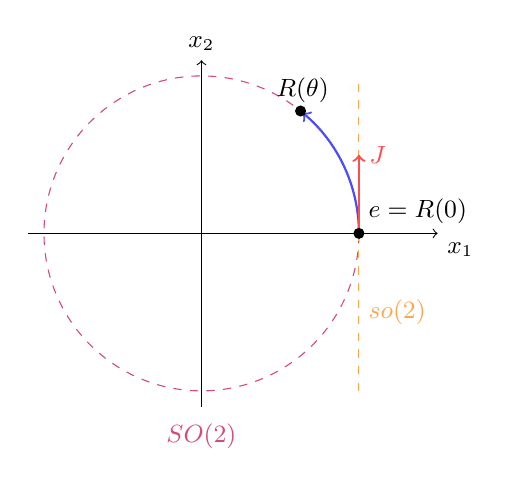
\begin{tikzpicture}[scale=1,every node/.style={font=\small}]
            \draw[->] (-2.2,0) -- (3,0) node[below right] {$x_1$};
            \draw[->] (0,-2.2) -- (0,2.2) node[above] {$x_2$};

            \draw[dashed, purple!70] (0,0) circle (2cm);
            \node[below, purple!70] at (0,-2.3) {$SO(2)$};

            \draw[->, thick, blue!70] (2,0) arc (0:50:2);
            \fill ({2*cos(51)},{2*sin(51)}) circle (2pt);
            \node[above] at ({2*cos(50)},{2*sin(50)}) {$R(\theta)$};

            \draw[dashed,orange!70] (2,-2) -- (2,2);
            \draw[->, red!70, thick] (2,0) -- +(0,1) node[right] {$J$};
            \node[right,orange!70] at (2,-1) {$\mathfrak{so}(2)$};

            \fill (2,0) circle (2pt) node[above right] {$e=R(0)$};
        \end{tikzpicture}
    \end{minipage}
\end{figure}

\textbf{Common Lie groups:}
\begin{itemize}
    \item $\mathbf{O(n)} = \{ R \in \mathbb{R}^{n \times n} \mid R^T R = I \}$: orthogonal group, preserves Euclidean lengths.
    \item $\mathbf{SO(n)} = \{ R \in O(n) \mid \det R = 1 \}$: special orthogonal group, proper rotations in $n$ dimensions.
    \item $\mathbf{U(n)} = \{ U \in \mathbb{C}^{n \times n} \mid U^\dagger U = I \}$: unitary group, preserves complex inner products.
    \item $\mathbf{SU(n)} = \{ U \in U(n) \mid \det U = 1 \}$: special unitary group, important for internal symmetries in particle physics.
          % \item $\mathbf{Sp(2n)} = \{ M \in \mathbb{R}^{2n \times 2n} \mid M^T \Omega M = \Omega \}$: symplectic group, preserves a symplectic form $\Omega$ in classical and quantum mechanics.
\end{itemize}

\subsection{Representations}

A \textbf{representation} of a Lie group or Lie algebra provides a concrete realization of its abstract elements as linear operators acting on a vector space.
Mathematically, a representation of a Lie group \(G\) is a homomorphism, for example
\[
    D : G \to \mathrm{GL}(V),
\]
where \(V\) is the vector space on which our representation is acting and \(\mathrm{GL}(V)\) denotes the group of invertible linear transformations on \(V\).
This means that the group law is preserved:
\[
    D(g_1 g_2) = D(g_1) D(g_2), \qquad \forall g_1,g_2 \in G.
\]
At the infinitesimal level, a representation of the associated Lie algebra \(\mathfrak{g}\) assigns to each generator \(T_a\) a linear operator \(D(T_a)\) such that
\[
    [D(T_a), D(T_b)] = i f_{ab}{}^{c} D(T_c),
\]
mirroring the structure constants \(f_{ab}{}^{c}\) of the algebra.

Representations are fundamental both in mathematics and in physics.
Mathematically, they allow us to study abstract symmetry groups through their action on vector spaces, revealing their structure via matrices or operators.
Physically, they describe how different objects transform under a given symmetry:
scalars correspond to the trivial (one-dimensional) representation,
vectors to the fundamental representation, and spinors or tensors to higher-dimensional or mixed representations.

Of particular importance are the \textbf{irreducible representations}, which cannot be decomposed into smaller invariant subspaces.
These play the role of the "elementary building blocks" of a group—just as elementary particles of definite spin are the basic excitations transforming irreducibly under spacetime symmetries.

Different Lie groups admit representations of various \textbf{dimensions}, depending on how the group acts on the underlying vector space.
For example, the group $SO(2)$ can be represented by $2\times 2$ rotation matrices acting on vectors in the plane, but also by complex phase factors $e^{i n \theta}$ acting on one-dimensional complex spaces, each labeled by an integer $n$.
In general, higher-dimensional representations describe systems that transform with more internal components---such as vectors, tensors, or spinors---while lower-dimensional ones correspond to simpler transformation laws.
The dimension of the representation thus reflects the number of independent degrees of freedom that transform under the symmetry.

\section{The Lorentz Group}

The most fundamental symmetry group in relativistic field theory is the \textbf{Lorentz group}, denoted by \(\mathrm{O}(1,3)\).
It consists of all linear transformations \(\Lambda: \mathbb{R}^{1,3} \to \mathbb{R}^{1,3}\) that leave the Minkowski metric invariant:
\[
    \eta_{\mu\nu} = \mathrm{diag}(1,-1,-1,-1),
\]
i.e.
\[
    \eta_{\mu\nu} \, \Lambda^{\mu}{}_{\rho} \Lambda^{\nu}{}_{\sigma} = \eta_{\rho\sigma}.
\]

These transformations preserve the spacetime interval
\[
    s^2 = \eta_{\mu\nu} x^\mu x^\nu = (x^0)^2 - \vec{x}^{\,2},
\]
or, infinitesimally,
\[
    \mathrm{d}s^2 = \eta_{\mu\nu} \, \mathrm{d}x^\mu \mathrm{d}x^\nu.
\]

Indeed, under a Lorentz transformation \(x^\mu \mapsto x'^\mu = \Lambda^\mu{}_\rho x^\rho\), we have
\[
    \begin{aligned}
        \mathrm{d}s'^2 & = \eta_{\mu\nu} \, \mathrm{d}x'^\mu \mathrm{d}x'^\nu
        = \eta_{\mu\nu} \, \Lambda^\mu{}_\rho \mathrm{d}x^\rho \, \Lambda^\nu{}_\sigma \mathrm{d}x^\sigma                     \\
                       & = \Lambda^\mu{}_\rho \, \eta_{\mu\nu} \, \Lambda^\nu{}_\sigma \, \mathrm{d}x^\rho \mathrm{d}x^\sigma
        = \eta_{\rho\sigma} \, \mathrm{d}x^\rho \mathrm{d}x^\sigma
        = \mathrm{d}s^2,
    \end{aligned}
\]
confirming that Lorentz transformations leave the Minkowski interval invariant.


The determinant of a Lorentz transformation can be either \(+1\) or \(-1\), and \(\Lambda^0{}_0\) can be greater or smaller than \(1\).
The subgroup with \(\det \Lambda = +1\) and \(\Lambda^0{}_0 \ge 1\) is called the \textbf{proper orthochronous Lorentz group}, denoted by \(\mathrm{SO}^+(1,3)\).
It is this connected component that is continuously connected to the identity and relevant for most applications in physics.

\subsection{Infinitesimal Transformations and Generators}

An infinitesimal Lorentz transformation can be written as
\[
    \Lambda^\mu{}_\nu = \delta^\mu{}_\nu + \omega^\mu{}_\nu, \qquad |\omega^\mu{}_\nu| \ll 1,
\]
with the condition
\[
    \eta_{\mu\nu} \Lambda^\mu{}_\rho \Lambda^\nu{}_\sigma = \eta_{\rho\sigma}
    \quad \Rightarrow \quad
    \omega_{\mu\nu} = -\omega_{\nu\mu}.
\]
Hence, \(\omega_{\mu\nu}\) is an antisymmetric tensor containing six independent parameters, corresponding to the six generators of the Lorentz algebra.

We can introduce a set of generators \(M_{\mu\nu}\) (antisymmetric in their indices) such that a general infinitesimal transformation acts on a four-vector \(x^\rho\) as:
\[
    x'^\rho = \left( \delta^\rho{}_\sigma + \frac{i}{2}\,\omega^{\mu\nu} (M_{\mu\nu})^\rho{}_\sigma \right) x^\sigma,
\]
as taylor expansion of
\[
    \Lambda^{\rho}{}_{\sigma} =  e^{\frac{i}{2}\,\omega^{\mu\nu} (M_{\mu\nu})^\rho{}_\sigma},
\]
where the generators of the group are
\[
    (M_{\mu\nu})^\rho_{\ \sigma} = -i \left( \eta_{\mu\sigma} \, \delta^\rho_{\ \nu} - \eta_{\nu\sigma} \, \delta^\rho_{\ \mu} \right),
\]

The commutation relations among the generators define the \textbf{Lorentz algebra} \(\mathfrak{so}(1,3)\):
\[
    [M_{\mu\nu}, M_{\rho\sigma}] = i \left(
    \eta_{\nu\rho} M_{\mu\sigma}
    - \eta_{\mu\rho} M_{\nu\sigma}
    + \eta_{\mu\sigma} M_{\nu\rho}
    - \eta_{\nu\sigma} M_{\mu\rho}
    \right).
\]

\subsection{Generators: Rotations and Boosts}

The six generators can be naturally separated into:
\[
    \begin{aligned}
        J_i & \equiv \frac{1}{2} \epsilon_{ijk} M_{jk} \quad &  & \text{(spatial rotations)}, \\
        K_i & \equiv M_{0i} \quad                            &  & \text{(Lorentz boosts)}.
    \end{aligned}
\]
In terms of these generators, the Lorentz algebra decomposes as:
\[
    [J_i, J_j] = i \epsilon_{ijk} J_k, \qquad
    [J_i, K_j] = i \epsilon_{ijk} K_k, \qquad
    [K_i, K_j] = -i \epsilon_{ijk} J_k.
\]
This structure reveals the non-compact nature of the Lorentz group: unlike spatial rotations, boosts do not form a compact subgroup, as rapidities are unbounded.\footnote{When we later discuss the relation between \(\mathrm{SO}^+(1,3)\) and \(\mathrm{SU}(2) \times \mathrm{SU}(2)\), this distinction will be important: \(\mathrm{SU}(2) \times \mathrm{SU}(2)\) is compact, whereas the proper orthochronous Lorentz group is not.}


For finite transformations, one can write:
\[
    R(\bs{\theta}) = e^{-i \bs{\theta}\cdot \mathbf{J}},
    \qquad
    B(\bs{\beta}) = e^{-i \bs{\beta}\cdot \mathbf{K}},
\]
where \(\bs{\theta} = \left( \theta_1,\,\theta_2,\,\theta_3 \right)\) are the rotation angles and \(\bs{\beta} = \left( \beta_1,\,\beta_2,\,\beta_3\right) \) the boost parameters. We can ultimately reconstruct the expression for \(\omega_{\mu\nu}\):
\[
    \begin{aligned}
        \omega_{ij} & = \epsilon_{ijk}\bs{\theta}^k, \\
        \omega_{0i} & = \bs{\beta}_i.
    \end{aligned}
\]
Together, they parametrize any proper orthochronous Lorentz transformation as a combination of a boost and a rotation:
\[
    \Lambda = B(\bs{\beta}) \, R(\bs{\theta}).
\]

\subsection{Representations}

The Lorentz algebra \(\mathfrak{so}(1,3)\) is locally isomorphic to the direct sum \(\mathfrak{su}(2) \oplus \mathfrak{su}(2)\) (algebra of $SU(2) \times SU(2)$, equivalent up to different hermiticity relations arising because of compactess).
This correspondence allows the classification of all finite-dimensional representations of the Lorentz group in terms of pairs \((j_+, j_-)\) of \(\mathrm{SU}(2)\) spins.

One can then construct the combinations
\[
    \mathbf{A} = \frac{1}{2} (\mathbf{J} + i \mathbf{K}), \qquad
    \mathbf{B} = \frac{1}{2} (\mathbf{J} - i \mathbf{K}),
\]
which satisfy independent \(\mathfrak{su}(2)\) algebras:
\[
    [A_i, A_j] = i \epsilon_{ijk} A_k, \quad
    [B_i, B_j] = i \epsilon_{ijk} B_k, \quad
    [A_i, B_j] = 0.
\]

This shows explicitly the algebra decompiìosition into a direct sum of two commuting algebras.
A concrete realization of the Lorentz algebra generators can be constructed using \textbf{spinor spaces}.
Consider spin-$\tfrac{1}{2}$ representations, and let \(\sigma_i\) denote the Pauli matrices.
Define the combinations
\[
    \mathbf{A} = \frac{1}{2} \boldsymbol{\sigma} \otimes \mathbf{1}, \qquad
    \mathbf{B} = \frac{1}{2} \mathbf{1} \otimes \boldsymbol{\sigma},
\]
which act on the four-dimensional space \(\mathbb{C}^2 \otimes \mathbb{C}^2\).

In this language, the \textbf{left-handed} (LH) \textbf{spinors} transform under the \((\tfrac{1}{2},0)\) representation, corresponding to the action of \(\mathbf{A}\) on the first factor, while the \textbf{right-handed} (RH) \textbf{spinors} transform under the \((0,\tfrac{1}{2})\) representation, corresponding to the action of \(\mathbf{B}\) on the second factor.

The Dirac spinor arises as the direct sum \(\psi = \psi_L \oplus \psi_R \in \mathbb{C}^2 \oplus \mathbb{C}^2\), and higher-dimensional representations of the Lorentz group can be constructed by taking tensor products of these spinor spaces, yielding \((j_+, j_-)\) representations with arbitrary spins.

\paragraph{Trivial representation.}
In addition to the nontrivial representations, every Lie group admits a trivial representation, denoted by $(0,0)$ in the $\mathrm{SU}(2)\times\mathrm{SU}(2)$ classification. In this representation, the group acts identically on the vector space: for any group element $g \in G$ and any vector $v$ in the representation space,
\[
    g \cdot v = v.
\]
The trivial representation is one-dimensional and corresponds to \textit{scalars} under the symmetry: objects that remain invariant under all group transformations, such as the Higgs field under Lorentz transformations.

Although the underlying representation space $\mathbb{C}^2 \otimes \mathbb{C}^2$ is the same, different choices of the $(j_+,j_-)$ representation allow us to classify distinct particles and fields according to their transformation properties under the Lorentz group, as shown in the following table.

\begin{table}[H]
    \centering
    \begin{tabular}{clc}
        \toprule
        Representation $(j_+,j_-)$               & Field / Particle type   & Total spin $s$ \\
        \midrule
        $(0,0)$                                  & Scalar                  & $0$            \\
        $\left(\tfrac{1}{2},0\right)$            & LH Weyl spinor          & $\tfrac{1}{2}$ \\
        $\left(0,\tfrac{1}{2}\right)$            & RH Weyl spinor          & $\tfrac{1}{2}$ \\
        $\left(\tfrac{1}{2},0\right)\oplus\left(0,\tfrac{1}{2}\right)$
                                                 & Dirac spinor            & $\tfrac{1}{2}$ \\
        $\left(\tfrac{1}{2},\tfrac{1}{2}\right)$ & Vector                  & $1$            \\
        $\left(1,\tfrac{1}{2}\right)\oplus\left(\tfrac{1}{2},1\right)$
                                                 & Rarita--Schwinger field & $\tfrac{3}{2}$ \\
        $(1,1)$                                  & Graviton                & $2$            \\
        \bottomrule
    \end{tabular}
\end{table}
The representations listed above correspond to the basic field types used in relativistic quantum field theory. Scalars describe spinless particles such as the Higgs boson. Weyl spinors transform under chiral representations of the Lorentz group, and their direct sum forms the Dirac spinor, which accounts for massive spin-$\tfrac{1}{2}$ fermions like the electron. The vector representation corresponds to spin-1 gauge bosons, such as the photon or gluons. The Rarita--Schwinger field describes spin-$\tfrac{3}{2}$ particles, notably the gravitino, while the symmetric rank-2 tensor representation corresponds to the graviton, a hypothetical spin-2 quantum of the gravitational field.

This representation theory is the foundation for classifying relativistic fields and particles by their transformation properties under the Lorentz group.

\subsection{Finite dimensional representations}

Finite-dimensional representations of the Lorentz group play a central role in quantum field theory, as they determine how physical fields transform under Lorentz transformations. These representations describe the intrinsic angular momentum (or \textit{spin}) content of fields. The Lorentz group itself is non-compact, and therefore it admits only non-unitary finite-dimensional representations. Such representations are classified according to the group isomorphism:
\[
    \mathrm{SO}^+(1,3) \simeq \mathrm{SL}(2,\mathbb{C})/\mathbb{Z}_2,
\]
and labeled by two half-integer indices \((j_L, j_R)\), corresponding respectively to the two \(\mathrm{SU}(2)\) factors in the decomposition
\[
    \mathrm{SL}(2,\mathbb{C}) \sim \mathrm{SU}(2)_L \times \mathrm{SU}(2)_R.
\]
We now review the most important finite-dimensional representations, relevant for relativistic field theory.

\subsubsection{Trivial representation}

The simplest representation is the \textbf{trivial representation}, in which all Lorentz generators vanish:
\[
    M^{\mu \nu} = 0 \implies \Lambda = e^{-\frac{i}{2}\omega_{\mu \nu}M^{\mu \nu}} = \mathbb{I}.
\]
It is a one-dimensional (\(1D\)) representation acting on scalar fields \(\phi\):
\[
    \phi \to \phi' = \Lambda \phi = \phi.
\]
Such a field is invariant under Lorentz transformations and is thus denoted by the label \((0,0)\). It represents a \textbf{spinless particle}, such as the Higgs boson or the pion field, when regarded as a function defined on spacetime. This representation captures fields that do not transform under spatial rotations or boosts.

\subsubsection{Vectorial representation}

The next non-trivial case is the \textbf{vectorial representation}, in which the Lorentz generators act on four-vectors \(V^\mu\) according to:
\[
    (M^{\rho \sigma})^{\mu}_{\ \nu} = -i \left( \eta^{\mu \sigma} \delta^{\rho}_{\ \nu} - \eta^{\rho \mu} \delta^{\sigma}_{\ \nu} \right).
\]
These are \(4 \times 4\) matrices generating transformations of the form:
\[
    V^{\mu} \to V'^{\mu} = \Lambda^{\mu}_{\ \nu} V^{\nu} = e^{-\frac{i}{2} \omega_{\rho \sigma} (M^{\rho \sigma})^{\mu}_{\ \nu}} V^{\nu}.
\]
This is the \((\tfrac{1}{2}, \tfrac{1}{2})\) representation, often referred to as the \textit{fundamental vector representation}. It describes spin–1 particles, such as gauge bosons (photon, gluon, \(W^\pm\), and \(Z\) bosons), whose classical fields transform as four-vectors under Lorentz transformations.

\subsubsection{Spinorial representation}

The \textbf{spinorial representations} of the Lorentz group are more subtle. The proper orthochronous Lorentz group \(\mathrm{SO}^+(1,3)\) is not simply connected, and its double cover is the group \(\mathrm{SL}(2,\mathbb{C})\):
\[
    Spin^+(1,3) \equiv \mathrm{SL}(2,\mathbb{C}), \qquad \mathrm{SO}^+(1,3) \simeq \mathrm{SL}(2,\mathbb{C})/\mathbb{Z}_2.
\]
This means that for every Lorentz transformation \(\Lambda \in \mathrm{SO}^+(1,3)\) there exist two elements \(\pm A \in \mathrm{SL}(2,\mathbb{C})\) corresponding to it, establishing a two-to-one homomorphism:
\[
    A, B \in \mathrm{SL}(2,\mathbb{C}) \quad \longrightarrow \quad \Lambda \in \mathrm{SO}^+(1,3), \qquad \Lambda(A)\Lambda(B) = \Lambda(AB).
\]
The spinorial representations of \(\mathrm{SL}(2,\mathbb{C})\) correspond to the half-integer spin representations of the Lorentz group.

We introduce the Hermitian matrices
\[
    \sigma^{\mu} = (\mathbb{I}, \boldsymbol{\sigma}),
\]
where \(\boldsymbol{\sigma} = (\sigma^1, \sigma^2, \sigma^3)\) are the \textbf{Pauli matrices}:
\[
    \sigma^1 = \begin{pmatrix} 0 & 1 \\ 1 & 0 \end{pmatrix}, \quad
    \sigma^2 = \begin{pmatrix} 0 & -i \\ i & 0 \end{pmatrix}, \quad
    \sigma^3 = \begin{pmatrix} 1 & 0 \\ 0 & -1 \end{pmatrix}.
\]
A spacetime point \(x^{\mu}\) can then be represented by a \(2\times2\) Hermitian matrix:
\[
    X = x_{\mu}\sigma^{\mu} =
    \begin{pmatrix}
        x_0 + x_3   & x_1 - i x_2 \\
        x_1 + i x_2 & x_0 - x_3
    \end{pmatrix}.
\]
Under a Lorentz transformation, this object transforms as
\[
    X \longrightarrow X' = N X N^{\dagger}, \qquad N \in \mathrm{SL}(2,\mathbb{C}),
\]
which preserves the Minkowski norm, since
\[
    \det X' = \det N \det X \det N^{\dagger} = \det X = x_{\mu} x^{\mu} = x_0^2 - |\mathbf{x}|^2.
\]
Thus, \(N\) and \(-N\) generate the same Lorentz transformation, explaining the double-cover structure:
\[
    N = \pm \mathbb{I}_2 \quad \longrightarrow \quad \Lambda = \mathbb{I}_4.
\]

\paragraph{Representations of \(\mathrm{SL}(2,\mathbb{C})\).}

We can now define two inequivalent fundamental spinor representations:

\begin{enumerate}
    \item \textbf{Left-handed Weyl spinors} (fundamental representation \((\tfrac{1}{2},0)\)):
          \[
              \psi_{\alpha} =
              \begin{pmatrix}
                  \psi_1 \\ \psi_2
              \end{pmatrix}
              \to
              \psi'_{\alpha} = N_{\alpha}^{\ \beta} \psi_{\beta}, \quad \alpha,\beta = 1,2.
          \]
          These two-component spinors transform under the left-handed subgroup \(\mathrm{SU}(2)_L\).

    \item \textbf{Right-handed Weyl spinors} (complex conjugate representation \((0,\tfrac{1}{2})\)):
          \[
              \bar{\chi}_{\dot{\alpha}} =
              \begin{pmatrix}
                  \bar{\chi}_{\dot{1}} \\ \bar{\chi}_{\dot{2}}
              \end{pmatrix}
              \to
              \bar{\chi}'_{\dot{\alpha}} = N_{\dot{\alpha}}^{* \dot{\beta}} \bar{\chi}_{\dot{\beta}}, \quad \dot{\alpha},\dot{\beta} = 1,2.
          \]
          These transform under the right-handed subgroup \(\mathrm{SU}(2)_R\).
\end{enumerate}

\begin{remark}
    In the Lorentz group \(\mathrm{SO}^+(1,3)\), indices are raised and lowered using the Minkowski metric \(\eta_{\mu\nu}\). In contrast, within \(\mathrm{SL}(2,\mathbb{C})\) spinor indices are manipulated using the antisymmetric invariant tensors \(\epsilon^{\alpha\beta}\) and \(\epsilon^{\dot{\alpha}\dot{\beta}}\):
    \[
        \epsilon^{\alpha \beta} = \epsilon^{\dot{\alpha}\dot{\beta}} =
        \begin{pmatrix}
            0  & 1 \\
            -1 & 0
        \end{pmatrix}.
    \]
    These are invariant under \(\mathrm{SL}(2,\mathbb{C})\) transformations:
    \[
        \epsilon^{\alpha \beta} = \epsilon^{\gamma \delta} N^{\ \alpha}_{\gamma} N^{\ \beta}_{\delta} = \epsilon^{\alpha \beta} \det N = \epsilon^{\alpha \beta},
    \]
    allowing the relations
    \[
        \psi^{\alpha} = \epsilon^{\alpha \beta} \psi_{\beta}, \qquad
        \bar{\chi}^{\dot{\alpha}} = \epsilon^{\dot{\alpha}\dot{\beta}} \bar{\chi}_{\dot{\beta}}.
    \]
\end{remark}

\paragraph{Generators.}
The infinitesimal generators of \(\mathrm{SL}(2,\mathbb{C})\) are given by:
\[
    \left\{
    \begin{aligned}
        (\sigma^{\mu \nu})_{\alpha}^{\ \beta}                   & = \frac{i}{4} (\sigma^{\mu} \bar{\sigma}^{\nu} - \sigma^{\nu} \bar{\sigma}^{\mu})^{\ \beta}_{\alpha},             \\
        (\bar{\sigma}^{\mu \nu})^{\dot{\alpha}}_{\ \dot{\beta}} & = \frac{i}{4} (\bar{\sigma}^{\mu} \sigma^{\nu} - \bar{\sigma}^{\nu} \sigma^{\mu})^{\dot{\alpha}}_{\ \dot{\beta}}.
    \end{aligned}
    \right.
\]
Thus,
\[
    \begin{aligned}
        \psi_{\alpha}             & \to e^{-\frac{i}{2}\omega_{\mu\nu}(\sigma^{\mu\nu})_{\alpha}^{\ \beta}}\psi_{\beta}, \quad                               & \text{(LH Weyl spinor)} \\
        \bar{\chi}^{\dot{\alpha}} & \to e^{-\frac{i}{2}\omega_{\mu\nu}(\bar{\sigma}^{\mu\nu})^{\dot{\alpha}}_{\ \dot{\beta}}}\bar{\chi}^{\dot{\beta}}, \quad & \text{(RH Weyl spinor)}
    \end{aligned}
\]

\paragraph{Dirac spinors.}
A \textbf{Dirac spinor} is a four-component object obtained as the direct sum of a left-handed and a right-handed Weyl spinor:
\[
    \Psi =
    \begin{pmatrix}
        \psi_{\alpha} \\
        \bar{\chi}^{\dot{\alpha}}
    \end{pmatrix}.
\]
This reducible representation contains four complex (or eight real) components and transforms as:
\[
    \Psi \to \Psi' = e^{-\frac{i}{2} \omega_{\mu \nu} \Sigma^{\mu \nu}} \Psi,
\]
where the generators in the \textit{Weyl basis} are
\[
    \Sigma^{\mu \nu} = \frac{i}{4} [\gamma^{\mu}, \gamma^{\nu}] =
    \begin{pmatrix}
        \sigma^{\mu \nu} & 0                      \\
        0                & \bar{\sigma}^{\mu \nu}
    \end{pmatrix},
\]
and the gamma matrices are defined as
\[
    \gamma^{\mu} =
    \begin{pmatrix}
        0                  & \sigma^{\mu} \\
        \bar{\sigma}^{\mu} & 0
    \end{pmatrix}.
\]

\paragraph{Chirality operator.}
The \textbf{chirality operator} is defined as
\[
    \gamma^5 = i \gamma^0 \gamma^1 \gamma^2 \gamma^3 =
    \begin{pmatrix}
        -\mathbb{I}_2 & 0            \\
        0             & \mathbb{I}_2
    \end{pmatrix}, \quad (\gamma^5)^2 = \mathbb{I}.
\]
It distinguishes the two Weyl components through its eigenvalues:
\[
    \gamma^5 \Psi =
    \begin{pmatrix}
        -\psi_{\alpha} \\
        \bar{\chi}^{\dot{\alpha}}
    \end{pmatrix},
\]
so that left-handed spinors have eigenvalue \(-1\), and right-handed ones \(+1\). For massless fermions, chirality coincides with helicity, i.e., the projection of spin along the direction of motion.

\paragraph{Chiral projectors.}
The corresponding projectors are:
\[
    P_L = \frac{\mathbb{I}_4 - \gamma^5}{2}, \qquad
    P_R = \frac{\mathbb{I}_4 + \gamma^5}{2},
\]
which isolate the left- and right-handed components:
\[
    P_L \Psi =
    \begin{pmatrix}
        \psi_{\alpha} \\ 0
    \end{pmatrix}, \qquad
    P_R \Psi =
    \begin{pmatrix}
        0 \\ \bar{\chi}^{\dot{\alpha}}
    \end{pmatrix}.
\]

\paragraph{Dirac conjugate.}
The Dirac conjugate spinor is defined by
\[
    \bar{\Psi} = \Psi^{\dagger} \gamma^0 =
    \begin{pmatrix}
        \chi^{\alpha} & \bar{\psi}^*_{\dot{\alpha}}
    \end{pmatrix},
\]
so that the complex conjugate of a left-handed spinor transforms as a right-handed one and vice versa.

\paragraph{Charge conjugation.}
Charge conjugation exchanges particles with their antiparticles. Using the charge conjugation matrix \(C\),
\[
    \Psi^c = C \bar{\Psi}^T =
    \begin{pmatrix}
        \chi^{\alpha} \\ \bar{\psi}^*_{\dot{\alpha}}
    \end{pmatrix}, \quad
    C = \begin{pmatrix}
        \epsilon_{\alpha \beta} & 0                                  \\
        0                       & \epsilon^{\dot{\alpha}\dot{\beta}}
    \end{pmatrix}.
\]
Under \(C\), a left-handed particle becomes a right-handed antiparticle, and vice versa.

\paragraph{Majorana spinors.}
A \textbf{Majorana spinor} is defined by the condition of being its own charge conjugate:
\[
    \Psi_M^c = \Psi_M \iff \psi_{\alpha} = \chi_{\alpha}.
\]
In this case,
\[
    \Psi_M =
    \begin{pmatrix}
        \psi_{\alpha} \\
        \bar{\psi}^{\dot{\alpha}}
    \end{pmatrix} =
    \begin{pmatrix}
        \psi_1 \\ \psi_2 \\ \psi^{*1} \\ \psi^{*2}
    \end{pmatrix}.
\]
A generic Dirac spinor can be expressed as a combination of two real Majorana spinors:
\[
    \Psi = \Psi_{M_1} + i\Psi_{M_2}, \quad \Psi^c = \Psi_{M_1} - i\Psi_{M_2}.
\]
No experimental evidence for fundamental Majorana fermions has been found so far, although neutrinos, being electrically neutral, are prime candidates for Majorana particles.

\subsection{Infinite dimensional representations}
\lipsum[1]

\subsubsection{Field representations}
\lipsum[1]

\subsubsection{One particle Hilbert space representation}
\lipsum[1]

\section{The Poincaré Group}

The \textbf{Poincaré group} is the fundamental symmetry group of relativistic spacetime.
It extends the Lorentz group by including spacetime translations, and thus encodes the full structure of special relativity:
\[
    x^{\mu} \to x'^{\mu} = \Lambda^{\mu}_{\ \nu} x^{\nu} + a^{\mu},
\]
where \(\Lambda\) is a Lorentz transformation and \(a^\mu\) a spacetime translation vector.
Hence, it is also called the \textit{inhomogeneous proper orthochronous Lorentz group}, often denoted as \(ISO^+(1,3)\).
In quantum field theory, the Poincaré group plays a central role: every isolated physical system must admit a unitary representation of this group on its Hilbert space, ensuring the invariance of the theory under rotations, boosts, and translations.

From an algebraic point of view, the Poincaré group is a \textbf{ten-parameter Lie group} generated by the four-momentum operators \(P_\mu\) (associated with translations) and the six Lorentz generators \(M_{\mu\nu}\) (associated with rotations and boosts), which satisfy the \textit{Poincaré algebra}:
\[
    [P^\mu, P^\nu] = 0, \qquad
    [M^{\mu\nu}, P^\sigma] = i \left(P^\mu \eta^{\nu\sigma} - P^\nu \eta^{\mu\sigma}\right),
\]
together with the usual Lorentz commutation relations for \(M^{\mu\nu}\).
The fact that the momentum operators commute among themselves shows that the translation subgroup is \textbf{abelian}. Physically, this reflects that momentum is additive and that free particles can be simultaneously diagonalized with respect to their energy and momentum. This also connects to gauge theories: interactions mediated by abelian gauge bosons (like the photon) do not self-interact, while non-abelian gauge bosons (like \(W\) and \(Z\) bosons) have self-interactions due to the non-commuting structure of their symmetry generators.

\paragraph{Field representation.} In the \textit{field representation}, the Poincaré generators act on fields as differential operators. In particular, spacetime translations are represented by
\[
    P^\mu = i \frac{\partial}{\partial x_\mu} = i \partial^\mu,
\]
so that a translation of a field \(\Phi(x)\) is realized as
\[
    \Phi(x) \to \Phi'(x) = e^{-i a_\mu P^\mu} \Phi(x) = \Phi(x + a).
\]
This makes explicit how continuous spacetime symmetries are represented by \textit{infinitesimal differential operators} acting on classical or quantum fields.

\subsection{Representations: one-particle Hilbert space}

The representation theory of the Poincaré group on the \textit{one-particle Hilbert space} provides the foundation for the relativistic description of quantum particles.
Each irreducible unitary representation corresponds to a distinct type of elementary particle, characterized by the eigenvalues of the Casimir operators that we are about to introduce.
This framework, originally developed by Wigner, unifies the treatment of spin and momentum in relativistic quantum mechanics and serves as the bridge between the abstract group-theoretic structure and the physical notion of particles.

\subsubsection{Casimir operators}

Recall that operators \(A\) that commute with a generator \(T\) of a symmetry represent conserved quantities under that transformation:
\[
    [A, T] = 0 \implies AT = TA.
\]
Explicitly, if \(\ket{\psi}\) is an eigenstate of \(A\):
\[
    A \ket{\psi} = a \ket{\psi},
\]
then under the transformation generated by \(T\):
\[
    \ket{\psi} \to \ket{\psi'} = e^{i \alpha T} \ket{\psi} = \left(\mathbb{I} + i \alpha T + \mathcal{O}(\alpha^2) \right) \ket{\psi},
\]
we have
\[
    \begin{aligned}
        A \ket{\psi'} & = A \left(\mathbb{I} + i \alpha T \right) \ket{\psi} = A \ket{\psi} + i \alpha A T \ket{\psi}      \\
                      & = a \ket{\psi} + i \alpha T A \ket{\psi} = a (\mathbb{I} + i \alpha T) \ket{\psi} = a \ket{\psi'}.
    \end{aligned}
\]
This shows that the eigenvalue \(a\) is invariant under the transformation: the conserved quantity remains the same.

An operator that commutes with all generators of a group is called a \textbf{Casimir operator}. Casimir operators are important because their eigenvalues are invariants that can be used to label irreducible representations, i.e., multiplets of states sharing the same conserved quantities.

For the Poincaré group, there are two independent Casimir operators:
\begin{equation}
    C_1 = P^\mu P_\mu, \qquad C_2 = W^\mu W_\mu,
    \label{eq:casimir_operators_poincare}
\end{equation}
where \(W_\mu\) is the \textbf{Pauli-Lubanski vector}:
\begin{equation}
    W_\mu = +\frac{1}{2} \epsilon_{\mu\nu\rho\sigma} P^{\nu} M^{\rho\sigma}.
    \label{eq:Pauli_Lubanski_vector}
\end{equation}

The physical interpretation is:

\begin{itemize}
    \item \(C_1 = P^\mu P_\mu\) corresponds to the squared mass of the particle. Since \(P_\mu\) commutes with itself and with all Lorentz generators, all states in an irreducible representation have the same mass.
    \item \(C_2 = W^\mu W_\mu\) is related to the intrinsic spin (for massive particles) or helicity (for massless particles). It provides a Lorentz-invariant characterization of the particle's rotational degrees of freedom.
\end{itemize}

Hence, different irreducible representations of the Poincaré group are classified by the eigenvalues of \(C_1\) and \(C_2\), giving a systematic way to organize particle types in relativistic quantum mechanics.

\subsubsection{Massive representation}

For \textbf{massive particles} (\(m > 0\)), the first Casimir operator of the Poincaré group satisfies
\[
    C_1 = P^{\mu} P_{\mu} = P^2, \quad \text{with eigenvalue } p^2 = E_{\mathbf{p}}^2 - |\mathbf{p}|^2 = m^2 \neq 0.
\]
This defines a family of states all having the same mass \(m\), obtained by applying the full set of Poincaré transformations to a chosen reference four-momentum \(p^{\mu}\). The resulting set of states can be denoted by \(\{p^\mu\}\), and a generic state can be initially labeled as \(\ket{m,\,p^\mu}\).

To classify these states further, we consider the second Casimir operator
\[
    C_2 = W^\mu W_\mu,
\]
where \(W_\mu\) is the Pauli-Lubanski vector defined in eq. \eqref{eq:Pauli_Lubanski_vector}.
Its eigenvalues are associated with intrinsic spin degrees of freedom of the particle.

\paragraph{Little group.}
To understand the internal structure, we fix \(p^\mu\) and look for all Poincaré generators that commute with \(P^\mu\). This subset of generators forms a subgroup of the Poincaré group called the \textit{little group}: this subgroup leaves the four-momentum \(p^\mu\) invariant and its representations classify the internal degrees of freedom of the particle, such as spin.

It is defined as the subgroup of Lorentz transformations \(\Lambda\) that leaves this vector unchanged:
\[
    \Lambda^{\mu}_{\ \nu} p^{\nu} = p^{\mu}.
\]

Importantly, Wigner showed that the structure of the little group does not depend on the specific choice of \(p^\mu\) within its equivalence class \(\{p^\mu\}\), allowing us to select the simplest frame for calculations: the rest frame
\[
    p^\mu = (m, 0, 0, 0).
\]

In the rest frame, it turns out that only the spatial rotation generators
\[
    J_i = \frac{1}{2} \epsilon_{ijk} M^{jk}, \quad i=1,2,3,
\]
commute with \(P^\mu\), so the little group is isomorphic to \(SO(3)\), the group of spatial rotations. In more complicated situations, finding the little group may require evaluating nontrivial commutators, but for massive particles in the rest frame the identification is straightforward.

\paragraph{Pauli-Lubanski vector.}
The Pauli-Lubanski vector components in the rest frame are
\[
    \begin{aligned}
        W_0 & = \frac{1}{2} \epsilon_{0\nu\rho\sigma} P^\nu M^{\rho\sigma} = \frac{1}{2} \epsilon_{00\rho\sigma} m M^{\rho\sigma} = 0,                              \\
        W_i & = \frac{1}{2} \epsilon_{i\nu\rho\sigma} P^\nu M^{\rho\sigma} = \frac{1}{2} \epsilon_{i0jk} m M^{jk} = - \frac{m}{2} \epsilon_{0ijk} M^{jk} = - m J_i,
    \end{aligned}
\]
where the antisymmetry of the Levi-Civita tensor ensures that terms with repeated indices vanish. We thus recover the familiar rotation generators \(J_i\), so we can hypothesize that \(W_\mu\) generates transformations which leave \(p^\mu\) invariant:
\[
    \begin{aligned}
        [W_\mu,\, P_\nu] & = \frac{1}{2} \epsilon_{\mu\alpha\beta\gamma} [P^\alpha M^{\beta\gamma},\, P_\nu] = \frac{1}{2} \epsilon_{\mu\alpha\beta\gamma} \eta_{\nu \rho} [P^\alpha M^{\beta\gamma},\, P^\rho]                                                                         \\
                         & = \frac{1}{2} \epsilon_{\mu\alpha\beta\gamma} \eta_{\nu \rho} \left( P^\alpha [M^{\beta\gamma},\, P^\rho] + [P^\alpha,\, P^\rho] M^{\beta\gamma} \right)                                                                                                     \\
                         & = \frac{1}{2} \epsilon_{\mu\alpha\beta\gamma} \eta_{\nu \rho} \left( P^\alpha i (P^{\beta} \eta^{\gamma \rho} - P^{\gamma} \eta^{\beta \rho}) + 0 M^{\beta\gamma} \right)                                                                                    \\
                         & =\frac{i}{2} \epsilon_{\mu\alpha\beta\gamma} P^\alpha \left( P^{\beta} \eta_{\nu \rho} \eta^{\gamma \rho} - P^{\gamma} \eta_{\nu \rho} \eta^{\beta \rho} \right)                                                                                             \\
                         & = \frac{i}{2} \epsilon_{\mu\alpha\beta\gamma} P^\alpha (P^{\beta} \delta_{\nu}^{\ \gamma} - P^{\gamma} \delta_{\nu}^{\ \beta}) = \frac{i}{2} \epsilon_{\mu\alpha\beta\nu} P^\alpha P^{\beta} - \frac{i}{2} \epsilon_{\mu\alpha\nu\gamma} P^\alpha P^{\gamma} \\
                         & = \frac{i}{2} \epsilon_{\mu\alpha\beta\nu} P^\alpha P^{\beta} + \frac{i}{2} \epsilon_{\mu\alpha\gamma\nu} P^\alpha P^{\gamma} = i \epsilon_{\mu\alpha\beta\nu} P^\alpha P^{\beta} = 0,
    \end{aligned}
\]
since \(P^\alpha P^{\beta}\) is symmetric while \(\epsilon_{\mu\alpha\beta\nu}\) is antisymmetric for exchange of \(\alpha\) and \(\beta\). This results hold for both massive and massless particles.

Consequently, the second Casimir operator reduces to
\[
    C_2 = W^\mu W_\mu = - m^2 \mathbf{J}^2,
\]
with \(\mathbf{J}^2\) the squared angular momentum operator. Its eigenvalues are
\[
    j(j+1), \quad j = 0, \frac{1}{2}, 1, \frac{3}{2}, \dots,
\]
while the eigenvalues of \(J_3\) are
\[
    j_3 = -j, -j+1, \dots, j-1, j.
\]

\paragraph{Labeling the multiplet.}
Each state in the massive representation can thus be labeled as
\[
    \ket{m,\, j,\, j_3,\, p^\mu},
\]
where \(m\) is the mass, \(j\) the total spin, \(j_3\) the spin projection along a chosen axis, and \(p^\mu\) the four-momentum. The first three labels classify the multiplet, encoding internal spin degrees of freedom, while \(p^\mu\) specifies the individual state within the multiplet.

This construction shows explicitly how internal symmetries of a particle, such as spin, are directly derived from spacetime symmetries, illustrating how the Poincaré group unifies the treatment of momentum and spin in relativistic quantum mechanics.

\subsubsection{Massless representation}

For \textbf{massless particles} (\(m = 0\)), the first Casimir operator of the Poincaré group satisfies
\[
    C_1 = P^{\mu} P_{\mu} = P^2, \quad \text{with eigenvalue } p^2 = E_{\mathbf{p}}^2 - |\mathbf{p}|^2 = m^2 = 0.
\]
This condition identifies all possible states having vanishing invariant mass, i.e.\ those lying on the light cone of momentum space. Such states correspond to particles moving at the speed of light, for which energy and momentum are related by \(E_{\mathbf{p}} = |\mathbf{p}|\).

As in the massive case, we must now understand how the internal structure of these states --- their intrinsic degrees of freedom --- emerges from the symmetries of spacetime. To this purpose, we again study the subgroup of the Poincaré group that leaves a reference four-momentum \(p^{\mu}\) invariant: the so-called \textbf{little group}.

\paragraph{Little group.}
To identify the little group, we fix a representative momentum \(p^{\mu}\) within the orbit of all lightlike four-momenta under Lorentz transformations. A convenient and symmetric choice is
\[
    p^{\mu} = (E, 0, 0, E),
\]
which describes a massless particle propagating along the \(z\)-axis with energy \(E\) and momentum magnitude \(|\mathbf{p}| = E\).

Geometrically, these transformations conserve the direction of motion of the particle (commute with \(p^\mu\)), but can include both rotations around that direction and certain ``null'' boosts that act as translations in the plane transverse to it. Algebraically, this subgroup turns out to be isomorphic to the two-dimensional Euclidean group \(\mathrm{ISO}(2)\), consisting of rotations and translations in a plane.

To see how this arises, we can exploit the fact that the Pauli--Lubanski vector \(W_{\mu}\) commutes with the four-momentum operator \([W_{\mu},\, P_{\nu}] = 0\). Therefore, the components of \(W_{\mu}\) provide a convenient way to identify the generators of the little group that leave \(p^{\mu}\) invariant. Let us explicitly compute these components in the chosen frame:
\[
    \begin{aligned}
        W_0 & = \frac{1}{2} \epsilon_{0\nu\rho\sigma} P^\nu M^{\rho\sigma} = \frac{1}{2} \epsilon_{0 0 \rho \sigma} E M^{\rho\sigma} + \frac{1}{2} \epsilon_{0 3 \rho \sigma} E M^{\rho\sigma} \\
            & = \frac{1}{2} \left(\epsilon_{0 3 1 2} E M^{12} + \epsilon_{0 3 2 1} E M^{21}\right)                                                                                             \\
            & = E \frac{1}{2} \left( M^{12} - M^{12} \right) = E J_3.
    \end{aligned}
\]
and similarly
\[
    \begin{aligned}
        W_1 & = -E \left( J_1 + K_2 \right), \\
        W_2 & = -E \left( J_2 - K_1 \right), \\
        W_3 & = -E J_3 = - W_0.
    \end{aligned}
\]
Thus, three independent combinations of the Lorentz generators appear naturally: \(J_3\), \(J_1 + K_2\), and \(J_2 - K_1\). The first corresponds to rotations around the direction of propagation, while the other two mix boosts and rotations in such a way that they act as “translations” in the plane orthogonal to the momentum.

We can confirm that these generators indeed satisfy the commutation relations of the \(\mathrm{ISO}(2)\) algebra:
\[
    \begin{aligned}
        [W_1,\, W_2] & = 0,         \\
        [W_3,\, W_1] & = - i E W_2, \\
        [W_3,\, W_2] & = i E W_1.
    \end{aligned}
\]
This algebra corresponds to the group of isometries of the two-dimensional Euclidean plane: \(W_1\) and \(W_2\) generate translations, while \(W_3\) generates rotations about the axis perpendicular to that plane. From a group-theoretical point of view, this means that the internal symmetry space of a massless particle is not spherical (as in the massive case, where it was associated to \(\mathrm{SO}(3)\)), but planar. The plane is the space orthogonal to the direction of motion, and the physical states are classified according to how they transform under rotations and translations within it.

If the eigenvalues of \(W_1\) and \(W_2\) are non-zero, the resulting representations are infinite-dimensional, because the translations generate a continuous family of states labeled by continuous parameters -- a manifestation of the non-compactness of the subgroup generated by \(W_1\) and \(W_2\). In contrast, \(W_3\) generates a compact subgroup corresponding to \(\mathrm{SO}(2)\), whose eigenvalues are discrete.

However, in nature, only the latter type of representations are realized: physical massless particles correspond to the case in which the eigenvalues of \(W_1\) and \(W_2\) vanish. This restriction eliminates the continuous degrees of freedom associated with the non-compact part of the little group, leading to finite-dimensional representations that are fully characterized by the eigenvalues of \(W_3\).

Such representations describe the internal rotational properties of massless particles — properties that will later be associated with \textit{helicity}, the projection of the spin along the direction of motion.

\paragraph{Helicity.}
In the physically relevant case where the transverse components of the Pauli--Lubanski vector vanish, i.e.\ by setting \(W_1 = W_2 = 0\), the remaining non-zero components simplify drastically:
\[
    \begin{aligned}
        W_0   & = - W_3 = E J_3,                              \\
        W_0   & = W^0 = E J_3 = W^3 = - W_3,                  \\
        W^\mu & = J_3 \left(E,\,0,\,0,\,E\right) = J_3 P^\mu.
    \end{aligned}
\]
This shows that \(W^\mu\) becomes proportional to the four-momentum \(P^\mu\), with the proportionality factor given by the operator \(J_3\), the generator of rotations around the direction of propagation.
In this limit, the only remaining internal degree of freedom is the projection of the spin along the momentum direction — a quantity known as the \textbf{helicity}.

The helicity operator is thus defined as
\[
    h = \frac{W_\mu P^\mu}{P^\nu P_\nu}.
\]
However, since for massless particles \(P^\nu P_\nu = 0\), this expression must be interpreted carefully. In practice, one considers the proportionality relation \(W_\mu = h\,P_\mu\), valid on the physical subspace of states with definite helicity.
The operator \(h\) therefore measures how the intrinsic angular momentum (spin) is aligned or anti-aligned with the momentum of the particle. Its eigenvalues \(h\) are discrete and can take integer or half-integer values depending on the spin of the field under consideration.

Physically, \(h>0\) corresponds to a particle whose spin points in the same direction as its momentum (\textit{right-handed} or positive helicity state), while \(h<0\) corresponds to the opposite alignment (\textit{left-handed} or negative helicity state). These two possibilities represent the only independent polarization states available to a massless particle, since there is no rest frame in which to define a third (longitudinal) polarization component.

The second Casimir operator of the Poincaré group,
\[
    C_2 = W^\mu W_\mu,
\]
vanishes identically in this case, \(C_2 = 0\), because \(W^\mu\) is proportional to the null vector \(P^\mu\). Thus, unlike the massive case where \(C_2 = -m^2 \mathbf{J}^2\) provided a discrete spin multiplet, here the intrinsic structure of the representation is fully captured by the helicity eigenvalue.

\paragraph{Labeling the multiplet.}
Each state in the massless representation can therefore be labeled as
\[
    \ket{0,\,0,\,p^\mu,\,\pm h} \equiv \ket{p^\mu,\, \pm h},
\]
where \(h\) denotes the helicity and \(p^\mu\) the four-momentum of the state. The sign \(\pm\) distinguishes the two helicity states corresponding to opposite spin alignments relative to the direction of motion.

Under a \textit{parity} transformation, which reverses spatial orientation (\(\mathbf{p} \to -\mathbf{p}\)), the helicity changes sign:
\[
    h \xrightarrow{P} -h.
\]
Hence, parity inversion exchanges right-handed and left-handed states.
For this reason, a complete relativistic theory must generally include both helicities in order to be invariant under the combined \textit{CPT} transformation\footnote{CPT stands for Charge conjugation (C), Parity inversion (P), and Time reversal (T).}.

In the Standard Model, different particle species correspond to different allowed helicities:
\[
    \begin{aligned}
        h = 0                & \quad \text{Higgs boson (scalar)},             \\
        h = \pm \tfrac{1}{2} & \quad \text{leptons and quarks (fermions)},    \\
        h = \pm 1            & \quad \text{photon and gluons (gauge bosons)}, \\
        h = \pm 2            & \quad \text{graviton (tensor boson)}.
    \end{aligned}
\]
The two helicity states \(\pm h\) thus correspond to the two independent polarization states of a massless field. For instance, in the case of the photon, they represent the right-handed and left-handed circular polarizations of light, which are experimentally observable and fundamental to our understanding of electromagnetism in quantum field theory.

\begin{remark}
    It is conceptually illuminating to note that, at its most fundamental level, quantum field theory is intrinsically a \textbf{massless theory}.
    The full Poincaré symmetry---which combines Lorentz invariance and spacetime translations---is naturally realized on representations with \(m=0\).
    Introducing a nonzero mass ``by hand'' would in fact \textit{bend} this symmetry, since a massive term explicitly selects a preferred reference frame (the rest frame) and breaks conformal invariance.

    From this viewpoint, all fundamental fields are most naturally described as massless excitations of underlying quantum fields, each transforming under irreducible representations of the Poincaré group.
    Mass then arises dynamically through interaction with the scalar Higgs field: the Higgs mechanism endows particles with an effective rest mass while preserving the local gauge and Lorentz symmetries of the theory.
    This elegant construction reconciles the need for mass with the fundamental symmetry principles that govern relativistic quantum dynamics.
\end{remark}


% === Classical Field Theory ===
\chapter{Classical Field Theory}

In classical field theory there is a fundamental shift of perspective:
we move from describing a physical system through a \textit{finite} set of discrete trajectories evolving in time to describing it through a \textit{continuous} entity that takes different values at each point in space and evolves in time — the \textbf{field}.
This transition reflects the passage from a mechanics of point-like objects to a mechanics of distributed quantities, where energy, momentum, or charge may be continuously spread over space.

\begin{itemize}
    \item \textbf{Classical particle mechanics}

          In classical mechanics, the state of a system with \(N\) particles is determined by its \textit{generalized coordinates}
          \[
              q_i(t),
          \]
          together with their time derivatives \(\dot{q}_i(t)\).
          Each coordinate \(q_i\) specifies the position (or a suitable generalized coordinate) of the \(i\)-th degree of freedom at a given time \(t\).
          The system therefore possesses a \textit{finite} number of degrees of freedom, labelled by
          \[
              i = 1, \dots, N.
          \]
          The evolution of the system is then described by a set of ordinary differential equations in time — typically the Euler–Lagrange equations derived from a Lagrangian \(L(q_i, \dot{q}_i, t)\).

    \item \textbf{Classical field theory}

          In classical field theory, the basic object is a \textit{field}
          \[
              \psi_i(t, \mathbf{x}),
          \]
          which assigns a value (scalar, vector, or tensor) to each point in space and time.
          The field contains an \textit{infinite} number of degrees of freedom: the discrete index \(i = 1, \dots, N\) labels internal components (for example, the components of the electromagnetic or spinor field), while the continuous variable \(\mathbf{x}\) plays the role of a label identifying each point in space.
          The dynamics are now governed by \textit{partial differential equations} derived from a Lagrangian density \(\mathcal{L}(\psi_i, \partial_\mu \psi_i, x^\mu)\), which generalizes the Lagrangian of particle mechanics.
\end{itemize}

In this framework, the notion of a particle \textit{trajectory} loses its meaning.
There is no single path to follow: the field as a whole evolves, deforming continuously in space and time.
What acquires physical significance is therefore not the position of an individual object, but the \textit{configuration of the field} — the collective state of the system at each instant.
Classical field theory thus provides the natural language for describing systems where locality, continuity, and symmetry play a fundamental role, setting the conceptual foundation upon which modern relativistic and quantum field theories are built.

\section{Action and Lagrangian Density}

In classical field theory, the dynamics of a field \(\psi_i(t, \mathbf{x}) = \psi(x)\)\footnote{We will use the compact 4-vector notation \(x^\mu = (t, \mathbf{x})\).} are encoded in the \textbf{Lagrangian density} \(\mathcal{L}\), which is a functional of the fields, their first derivatives, and possibly the spacetime coordinates:
\[
    \mathcal{L} = \mathcal{L}(\psi_i, \partial_\mu \psi_i,  x^\mu),
\]
where \(\partial_\mu \psi_i = \frac{\partial \psi_i}{\partial x^\mu}\) denotes the spacetime derivative of the field.
In this formulation, the Lagrangian density depends only on \textit{first derivatives} of the fields — analogously to classical particle mechanics, where the Lagrangian depends on positions and velocities but not on accelerations.
Allowing higher-order derivatives would, in general, lead to fourth-order equations of motion and to instabilities (known as Ostrogradsky instabilities), hence such terms are typically excluded from physically meaningful theories.

The \textbf{action} \(S\) is then defined as the spacetime integral of the Lagrangian density:
\[
    S[\psi_i] = \int \mathrm{d}^4 x \, \mathcal{L}(\psi_i, \partial_\mu \psi_i, x^\mu),
\]
where \( \mathrm{d}^4 x = \mathrm{d}t \, \mathrm{d}^3\mathbf{x} \) in Minkowski spacetime.
The action is a scalar quantity under Lorentz transformations and encapsulates the full dynamics of the system.
The physical evolution of the fields will be determined by the principle of stationary action, discussed later on.

\subsection{Units and Dimensional Analysis}

It is often useful to analyze the Lagrangian density in terms of \textbf{mass dimensions}, especially when comparing different interaction terms.
Working in natural units, where \(\hbar = c = 1\), the action is dimensionless:
\[
    [S] = 0.
\]
Since the differential measure in \(3+1\) dimensions has dimension
\[
    [\mathrm{d}^4 x] = [L^4] = [M^{-4}] \coloneqq -4,
\]
the Lagrangian density must have mass dimension
\[
    [\mathcal{L}] = [M^4] = 4.
\]
This fact constrains the allowed forms of the Lagrangian and determines the mass dimensions of fields and coupling constants.

\paragraph{Example: Klein--Gordon Field.}
Consider the free scalar field described by the Klein–Gordon Lagrangian:
\[
    \mathcal{L} = \frac{1}{2}\, \partial_\mu \psi \, \partial^{\mu} \psi - \frac{1}{2} m^2 \psi^2.
\]
Each term in \(\mathcal{L}\) must have the same mass dimension, \( [\mathcal{L}] = 4 \).
Since derivatives have dimension \([\partial_\mu] = 1\), we can deduce the dimension of the scalar field:
\[
    4 = [\mathcal{L}] = 2[\partial_\mu] + 2[\psi] = 2 + 2[\psi] \quad \Rightarrow \quad [\psi] = 1.
\]
\paragraph{Interaction Terms and Couplings.}
If we extend the Lagrangian by including interaction terms,
\[
    \mathcal{L}' = \mathcal{L} + g\, \psi^3 - \lambda\, \psi^4,
\]
then the requirement \([\mathcal{L}'] = 4\) implies:
\[
    [g] = 4 - 3[\psi] = 1, \qquad [\lambda] = 4 - 4[\psi] = 0.
\]
Couplings with positive or zero mass dimension (\( [g] \ge 0 \)) correspond to \textbf{renormalizable} interactions, whereas those with negative mass dimension would lead to non-renormalizable theories, whose predictive power breaks down at high energies.

In summary, dimensional analysis plays a crucial role in identifying which interaction terms yield consistent and physically meaningful field theories.
Renormalizable theories — those with interaction terms up to fourth order in the fields in \(3+1\) dimensions — are the backbone of modern particle physics, while higher-order terms typically appear as effective corrections suppressed by powers of a large mass scale.

\subsection{The Variational Principle}

The evolution of a classical field is determined by the \textbf{principle of stationary action} (or \textbf{principle of least action}).
According to this principle, the physical configuration of the field \(\psi_i(x)\) is the one that makes the action \(S[\psi_i]\) stationary under small variations \(\delta \psi_i(x)\) that vanish at the boundaries:
\[
    \delta S = 0.
\]
In other words, among all possible field configurations that interpolate between two fixed states at times \(t_1\) and \(t_2\), the physical field follows the path in configuration space that extremizes the action functional. This generalizes the least-action principle of classical mechanics to systems with infinitely many degrees of freedom.

Starting from the definition of the action,
\[
    S[\psi_i] = \int \mathrm{d}^4x \, \mathcal{L}(\psi_i, \partial_\mu \psi_i, x^\mu),
\]
we consider an infinitesimal variation of the fields:
\[
    \psi_i(x) \longrightarrow \psi_i(x) + \delta \psi_i(x),
\]
with \(\delta \psi_i(x)\) assumed to vanish at the spacetime boundaries:
\[
    \delta \psi_i(t_1, \mathbf{x}) = \delta \psi_i(t_2, \mathbf{x}) = 0, \qquad \delta \psi_i(x) \to 0 \ \text{as} \ |x| \to \infty.
\]
These boundary conditions express the physical idea that there is no relevant dynamics infinitely far away in space or time — equivalently, that the field configuration is fixed at the initial and final times.

The variation of the action then reads:
\[
    \delta S = \int \mathrm{d}^4x \,
    \left[
        \frac{\partial \mathcal{L}}{\partial \psi_i} \, \delta \psi_i
        + \frac{\partial \mathcal{L}}{\partial (\partial_\mu \psi_i)} \, \delta(\partial_\mu \psi_i)
        \right].
\]
Since the variation and the derivative commute, we can rewrite:
\[
    \delta(\partial_\mu \psi_i) = \partial_\mu (\delta \psi_i),
\]
so that
\[
    \delta S = \int \mathrm{d}^4x \,
    \left[
        \frac{\partial \mathcal{L}}{\partial \psi_i} \, \delta \psi_i
        + \frac{\partial \mathcal{L}}{\partial (\partial_\mu \psi_i)} \, \partial_\mu (\delta \psi_i)
        \right].
\]

To isolate the variation \(\delta \psi_i\), we integrate the second term by parts using the product rule:
\[
    \frac{\partial \mathcal{L}}{\partial (\partial_\mu \psi_i)} \, \partial_\mu (\delta \psi_i)
    = \partial_\mu \!\left( \frac{\partial \mathcal{L}}{\partial (\partial_\mu \psi_i)} \, \delta \psi_i \right)
    - \partial_\mu \!\left( \frac{\partial \mathcal{L}}{\partial (\partial_\mu \psi_i)} \right) \delta \psi_i.
\]
The first term is a total divergence and can be converted, via Gauss's theorem, into a surface integral over the boundary \(\partial \mathcal{R}\) of the integration region \(\mathcal{R}\) (the region where \(\mathbf{x} \in ]-\infty,\,\infty[,\, t \in [t_1,\,t_2]\)):
\[
    \int_{\mathcal{R}} \mathrm{d}^4x \, \partial_\mu A^\mu
    = \oint_{\partial \mathcal{R}} \mathrm{d}\sigma_\mu \, A^\mu,
    \qquad
    A^\mu = \frac{\partial \mathcal{L}}{\partial (\partial_\mu \psi_i)} \, \delta \psi_i.
\]
Because the variations \(\delta \psi_i\) vanish at the boundary, this surface term gives no contribution.
Therefore, the variation of the action reduces to:
\[
    \delta S = \int \mathrm{d}^4x \,
    \left[
        \frac{\partial \mathcal{L}}{\partial \psi_i}
        - \partial_\mu \!\left( \frac{\partial \mathcal{L}}{\partial (\partial_\mu \psi_i)} \right)
        \right]
    \delta \psi_i.
\]

Since the variations \(\delta \psi_i\) are arbitrary within the integration region, the only way for \(\delta S\) to vanish is for the quantity in brackets to be zero everywhere.
This yields the \textbf{Euler--Lagrange equations for fields}:
\begin{equation}
    \boxed{
        \partial_\mu \left( \frac{\partial \mathcal{L}}{\partial (\partial_\mu \psi_i)} \right)
        - \frac{\partial \mathcal{L}}{\partial \psi_i} = 0.
    }
    \label{eq:euler_lagrange_fields}
\end{equation}

These are the fundamental \textbf{equations of motion} of classical field theory.
They generalize the Euler--Lagrange equations of particle mechanics to continuous systems with infinitely many degrees of freedom, describing the local evolution of the field at every point in spacetime. The beauty of this formulation lies in its compactness: all of the dynamics — from wave equations to Maxwell’s equations and beyond — can be derived from a single scalar quantity, the action.

\paragraph{Hamiltonian formalism.}
While the Lagrangian framework is sufficient to formulate the \textit{Path Integral quantization scheme}, the \textit{Hamiltonian formalism} is required in order to impose \textbf{canonical commutation relations} among fields and their conjugate momenta.

We begin by defining the \textbf{momentum density} \(\pi^i(x)\) conjugate to the field \(\psi^i(x)\):
\[
    \pi^i(x) = \frac{\partial \mathcal{L}}{\partial \dot{\psi}_i(x)}.
\]
\QUESTION{What does dot psi represent here? Temporal partial derivative or total?}The Hamiltonian is then obtained through a \textit{Legendre transformation} of the Lagrangian density:
\[
    H = \int \mathrm{d}^3 x\, \mathcal{H},
    \qquad
    \mathcal{H} = \pi^i\dot{\psi}_i - \mathcal{L},
\]
where the time derivatives \(\dot{\psi}_i(x)\) are expressed in terms of the conjugate momenta \(\pi^i(x)\).

The goal of this construction is to recast the dynamics in terms of canonical variables \((\psi^i, \pi^i)\), so that the classical Poisson brackets can later be promoted to \textbf{quantum commutation relations}. In this framework, fields become operators acting on the Fock space that defines the quantum states of the theory.

\section{Noether's Theorem}

Symmetries play a central role in the formulation of physical theories: they represent the transformations that leave the form of the equations of motion—or equivalently, the action—unchanged.
In both Lagrangian mechanics and field theory, the existence of a continuous symmetry implies the conservation of a physical quantity, a deep correspondence established by \textbf{Noether's theorem}.

To clarify the different kinds of symmetries that may appear in a physical system, it is useful to distinguish between those acting on the \textit{spacetime coordinates} and those acting on the \textit{dynamical variables} of the field.

\begin{table}[H]
    \centering
    \footnotesize
    \begin{tabular}{lllll}
        \toprule
        \textbf{Category} & \textbf{Type}        & \textbf{Nature} & \textbf{Character} & \textbf{Examples}                                                              \\
        \midrule
        \multirow{5}{*}{\textbf{Spacetime}}
                          & Translational        & Global          & Continuous         & \(x^\mu \to x^\mu + a^\mu\)                                                    \\[2pt]
                          & Lorentz              & Global          & Continuous         & Rotations and boosts, \(\Lambda^\mu{}_\nu\)                                    \\[2pt]
                          & Poincaré             & Global          & Continuous         & Translations + Lorentz transformations                                         \\[2pt]
                          & General coordinate   & Local           & Continuous         & \(x^\mu \to x^{\prime\mu}(x)\) (curved spacetime invariance)                   \\[2pt]
                          & Discrete (C, P, T)   & Global          & Discrete           & \(P: \mathbf{x}\!\to\!-\mathbf{x}, \; T: t\!\to\!-t, \; C: \psi\!\to\!\psi^c\) \\[2pt]
                          & Discrete \(P(x)\)    & Local           & Discrete           & \(P(x): \mathbf{x}\!\to\!-\mathbf{x}\)                                         \\[2pt]
                          & Supersymmetry (SUSY) & Global          & Continuous         & \(Q_\alpha, \bar{Q}_{\dot{\alpha}}\): mix bosons and fermions                  \\[2pt]
        \midrule
        \multirow{6}{*}{\textbf{Internal}}
                          & Phase symmetry       & Global          & Continuous         & \(U(1)_F: \psi \to e^{i\alpha}\psi\) (fermion number)                          \\[2pt]
                          & Flavor symmetry      & Global          & Continuous         & \(U(1)_F,\; SU(3)_F\): fermion flavor rotations                                \\[2pt]
                          & Gauge symmetry       & Local           & Continuous         & \(U(1),\, SU(2),\, SU(3)\) (QED, weak, strong)                                 \\[2pt]
                          & Standard Model       & Local           & Continuous         & \(SU(3)_c \times SU(2)_L \times U(1)_Y\)                                       \\[2pt]
                          & Discrete internal    & Global          & Discrete           & \(\mathbb{Z}_2,\, \mathbb{Z}_N\) (Ising, parity sectors)                       \\[2pt]
                          & Local discrete       & Local           & Discrete           & \(\mathbb{Z}_2(x)\): position-dependent sign flip                              \\[2pt]
        \bottomrule
    \end{tabular}
    \caption{Classification of spacetime and internal symmetries in classical and quantum field theory.}
    \label{tab:symmetries}
\end{table}
\begin{remark}
    Spacetime symmetries act on the coordinates \(x^\mu\) and define the kinematical structure of the theory, while internal symmetries act on field components at fixed spacetime points, relating distinct internal degrees of freedom. Continuous global symmetries give rise to conserved currents via Noether’s theorem, while local symmetries require the introduction of gauge fields to preserve invariance.
\end{remark}

Such symmetries can be \textbf{continuous}, like rotations or translations, or \textbf{discrete}, such as parity or charge conjugation.
In the case of continuous transformations, infinitesimal variations of the action lead naturally to conserved quantities, whose explicit form depends on the invariance properties of the Lagrangian density.
The precise relation between symmetry and conservation law is established by Noether’s theorem.

\paragraph{Symmetries and constraints on the Lagrangian.}
Requiring that the Lagrangian be invariant under a given symmetry transformation imposes nontrivial constraints on its structure. Invariance means that
\[
    \mathcal{L}(\phi, \partial_\mu \phi) = \mathcal{L}(\phi', \partial_\mu \phi'),
\]
so only specific combinations of fields and their derivatives are allowed. In other words, symmetries restrict the admissible terms that can appear in the Lagrangian. For instance, a global \(U(1)\) phase invariance forbids terms like \(\phi^2\) but allows \(|\phi|^2\). When the symmetry is promoted from global to local, i.e.\ the transformation parameter becomes space–time dependent, \(\alpha = \alpha(x)\), the original Lagrangian typically loses its invariance. To restore it, one must introduce new compensating fields—gauge fields—whose dynamics and couplings are dictated by the symmetry itself. This mechanism naturally induces interaction terms between matter and gauge fields, such as the electromagnetic coupling \(e \bar{\psi} \gamma^\mu A_\mu \psi\) in Quantum Electrodynamics. Thus, symmetries not only constrain the form of the Lagrangian but also determine the possible interactions among fields.

Let us now formulate Noether's theorem in the context of quantum field theory.

\begin{theorem}[Noether's theorem]
    Every continuous symmetry of the Lagrangian density \(\mathcal{L}\) gives rise to a \textbf{conserved current} \(J^{\mu}(x)\). The Euler--Lagrange equations of motion imply the local continuity equation:
    \begin{equation}
        \partial_\mu J^{\mu} (x) = 0,
        \label{eq:continuity}
    \end{equation}
    or equivalently
    \[
        \ddt{J^0} + \nabla \cdot \mathbf{J} = 0,
    \]
    which expresses the conservation of a physical quantity associated with the symmetry.
\end{theorem}

\begin{corollary}[Conserved charge]
    Given a conserved current \(J^\mu(x)\) satisfying eq.~\eqref{eq:continuity}, one can define the corresponding \textbf{conserved charge}:
    \begin{equation}
        Q = \int_{\mathbb{R}^3} \mathrm{d}^3 \mathbf{x}\, J^0(x),
        \label{eq:Noether_charge}
    \end{equation}
    which is constant in time provided the current vanishes sufficiently fast at spatial infinity.
\end{corollary}

\begin{proof}
    Taking the time derivative of \(Q\), we have:
    \[
        \frac{\mathrm{d}Q}{\mathrm{d}t} = \int_{\mathbb{R}^3} \mathrm{d}^3\mathbf{x}\, \ddt{J^0}
        = - \int_{\mathbb{R}^3}\mathrm{d}^3\mathbf{x}\, \nabla \cdot \mathbf{J}
        = - \oint_{\partial \mathbb{R}^3} \mathrm{d}\mathbf{s} \cdot \mathbf{J}.
    \]
    If the spatial current \(\mathbf{J}\) vanishes at infinity, the surface term disappears and \(\dot{Q}=0\). Therefore, \(Q\) is conserved in time.
\end{proof}

This conservation law can also be interpreted as a \textbf{local conservation}: within a finite volume \(V\),
\[
    \frac{\mathrm{d}Q_V}{\mathrm{d}t} = \int_{V} \mathrm{d}^3\mathbf{x}\, \ddt{J^0} = - \oint_{\partial V} \mathrm{d}\mathbf{s} \cdot \mathbf{J},
\]
meaning that any variation of the charge inside \(V\) is exactly compensated by the flux of \(\mathbf{J}\) across its boundary.

\subsection{Proof of Noether's theorem}

To prove Noether’s theorem, we start by considering a \textit{continuous infinitesimal transformation} of the field variables:
\begin{equation}
    \psi_i \to \psi_i' = \psi_i + \delta \psi_i,
    \label{eq:infinitesimal_transformation}
\end{equation}
where \(\delta \psi_i\) is assumed to be infinitesimally small.
Under this transformation, the Lagrangian density changes as
\[
    \mathcal{L} \to \mathcal{L}' = \mathcal{L} + \delta \mathcal{L}.
\]
If the theory is invariant under the transformation, the variation of the Lagrangian must be expressible as the \textit{total derivative} of a four-vector function \(K^{\mu}(\psi_i)\):
\[
    \delta \mathcal{L} = \partial_{\mu} K^{\mu}(\psi_i),
\]
so that the corresponding action
\[
    S = \int \mathrm{d}^4 x\, \mathcal{L}
\]
remains unchanged:
\[
    S' = S + \int \mathrm{d}^4x\, \delta \mathcal{L} = S + \int \mathrm{d}^4x\, \partial_\mu K^\mu(\psi_i) = S,
\]
since the surface term vanishes at infinity.
This expresses the physical requirement that \(\mathcal{L}\) and \(\mathcal{L}'\) describe the same dynamics.

Now, let us compute the variation of the Lagrangian explicitly. Using the chain rule, we have
\[
    \begin{aligned}
        \delta \mathcal{L}
         & = \frac{\partial \mathcal{L}}{\partial \psi_i} \, \delta \psi_i
        + \frac{\partial \mathcal{L}}{\partial (\partial_\mu \psi_i)} \, \delta (\partial_\mu \psi_i)             \\
         & = \frac{\partial \mathcal{L}}{\partial \psi_i} \, \delta \psi_i
        + \partial_\mu \!\left( \frac{\partial \mathcal{L}}{\partial (\partial_\mu \psi_i)} \, \delta \psi_i \right)
        - \partial_\mu \!\left( \frac{\partial \mathcal{L}}{\partial (\partial_\mu \psi_i)} \right) \delta \psi_i \\
         & = \delta \psi_i \left[ \frac{\partial \mathcal{L}}{\partial \psi_i}
            - \partial_\mu \!\left( \frac{\partial \mathcal{L}}{\partial (\partial_\mu \psi_i)} \right) \right]
        + \partial_\mu \!\left( \frac{\partial \mathcal{L}}{\partial (\partial_\mu \psi_i)} \, \delta \psi_i \right).
    \end{aligned}
\]
In the second line we used the product rule for derivatives, and in the third we isolated a total divergence term.
By the Euler–Lagrange equations for fields,
\[
    \frac{\partial \mathcal{L}}{\partial \psi_i}
    - \partial_\mu \!\left( \frac{\partial \mathcal{L}}{\partial (\partial_\mu \psi_i)} \right) = 0,
\]
the first term in brackets vanishes, leaving
\[
    \delta \mathcal{L} = \partial_\mu \!\left( \frac{\partial \mathcal{L}}{\partial (\partial_\mu \psi_i)} \, \delta \psi_i \right)
    = \partial_\mu K^\mu(\psi_i).
\]

Since both expressions for \(\delta \mathcal{L}\) represent total divergences, we can equate them and obtain
\[
    \partial_\mu \!\left( \frac{\partial \mathcal{L}}{\partial (\partial_\mu \psi_i)} \, \delta \psi_i - K^\mu(\psi_i) \right) = 0.
\]
Thus, the quantity inside the parentheses defines a \textbf{conserved current}:
\begin{equation}
    J^{\mu} = \frac{\partial \mathcal{L}}{\partial (\partial_\mu \psi_i)} \, \delta \psi_i - K^{\mu}(\psi_i),
    \label{eq:Noether_current}
\end{equation}
which satisfies \(\partial_\mu J^{\mu} = 0\).

Finally, for strictly invariant Lagrangians (\(\delta \mathcal{L} = 0\)), the term \(K^{\mu}\) vanishes identically, yielding this particular expression for the conserved current:
\[
    J^{\mu} = \frac{\partial \mathcal{L}}{\partial (\partial_\mu \psi_i)} \, \delta \psi_i.
\]

\begin{remark}
    The essential mathematical step of Noether’s theorem is recognizing that a continuous symmetry corresponds to an infinitesimal field transformation under which the Lagrangian changes by a total derivative. This guarantees the existence of a four-vector \(J^\mu\) whose divergence vanishes identically, establishing a one-to-one correspondence between continuous symmetries and conserved quantities.
\end{remark}

\section{Energy--Momentum Tensor}

In classical mechanics, invariance under spatial translations leads to the conservation of linear momentum, while invariance under time translations yields the conservation of energy.
We now explore how this idea generalizes in the framework of quantum field theory.

\subsection{Infinitesimal spacetime translations}

Let us consider an \textit{infinitesimal spacetime translation}.
Starting from a general Poincaré transformation,
\[
    x^{\nu} \to x^{\prime\,\nu} = \Lambda^{\nu}_{\ \mu} x^{\mu} + a^{\nu},
\]
we restrict to the case in which there is no Lorentz transformation (\(\Lambda^{\nu}_{\ \mu} = \delta^{\nu}_{\ \mu}\)),
and \(a^{\nu} = \epsilon^{\nu}\) is an infinitesimal constant displacement.
In this case, the transformation acts on the field as a \textbf{scalar transformation}:
\begin{equation}
    \psi_i(x) \to \psi_i^{\prime}(x)
    = \psi_i(x^{\nu} + \epsilon^{\nu})
    = \psi_i(x) + \epsilon^{\nu}\partial_{\nu}\psi_i(x),
    \label{eq:infinitesimal_spacetime_translation}
\end{equation}
where we expanded to first order in \(\epsilon^{\nu}\).

\subsubsection*{Active and passive viewpoints}

It is important to distinguish between two equivalent but conceptually different interpretations of a transformation: the \textit{active} and the \textit{passive} viewpoints. Although they lead to the same mathematical result, they differ in what is considered to be ``moved'' — the field or the coordinate system — and this can be counterintuitive at first.

\begin{itemize}
    \item \textbf{Active transformation:} the field configuration itself is displaced in spacetime, while the coordinates remain fixed. In this picture,
          \[
              \psi_i^{\prime}(x^{\prime}) = \psi_i(x),
          \]
          meaning that what changes is the \textit{physical field}, which is ``pushed forward'' along the translation vector \(\epsilon^{\nu}\).
          One can imagine taking the same field profile and sliding it through spacetime without altering its shape.

    \item \textbf{Passive transformation:} here, we view the change as a relabeling of the coordinate system rather than a motion of the field itself:
          \[
              \psi_i^{\prime}(x) = \psi_i(x^{\prime}).
          \]
          The field configuration is left untouched, but the coordinate grid used to describe it has been shifted by \(\epsilon^{\nu}\).
          Consequently, the field \textit{appears} to change its functional form when expressed in the new coordinates.
\end{itemize}

Although the two interpretations seem opposite — one moves the field, the other moves the coordinates — they are mathematically equivalent.
The difference lies only in our point of view: in one case we deform the object within a fixed frame, in the other we deform the frame itself.
This equivalence is crucial in field theory, where symmetries are often expressed in one language or the other depending on convenience.

\subsection{Variation of the Lagrangian}

Since the Lagrangian density \(\mathcal{L}\) is a scalar function of the fields and their derivatives,
\(\mathcal{L} = \mathcal{L}(\psi_i(x), \partial_{\mu}\psi_i(x))\),
its transformation under \eqref{eq:infinitesimal_spacetime_translation} follows as
\[
    \mathcal{L}(x) \to \mathcal{L}^{\prime}(x)
    = \mathcal{L}(x) + \epsilon^{\nu}\partial_{\nu}\mathcal{L}(x).
\]
Therefore, its infinitesimal variation reads
\[
    \delta \mathcal{L} = \mathcal{L}^{\prime} - \mathcal{L}
    = \epsilon^{\nu}\partial_{\nu}\mathcal{L}(x).
\]
It is often convenient to rewrite this expression as a total divergence:
\[
    \delta \mathcal{L}
    = \epsilon^{\nu}\partial_{\mu}(\delta^{\mu}_{\ \nu}\mathcal{L})
    = \partial_{\mu}(\epsilon^{\nu}\delta^{\mu}_{\ \nu}\mathcal{L}).
\]
The introduction of the Kronecker symbol \(\delta^{\mu}_{\ \nu}\) has no numerical effect, since
\(\partial_{\mu}(\delta^{\mu}_{\ \nu}\mathcal{L}) = \partial_{\nu}\mathcal{L}\);
its purpose is purely formal, allowing us to display explicitly the divergence index \(\mu\).
This step makes the expression ready for application of Noether’s theorem,
since a variation that can be written as a total divergence directly corresponds to a conserved current.

The four independent spacetime translations (one temporal and three spatial)
therefore yield four conserved quantities, which we will identify shortly as the components of the \textbf{four-momentum}.

\subsection{Noether current and charges}

Using the general expression for the Noether current derived in eq.~\eqref{eq:Noether_current},
we have
\[
    (J^{\mu})_{\nu}
    = \frac{\partial \mathcal{L}}{\partial (\partial_{\mu}\psi_i)}\,\delta\psi_i
    - K^{\mu}(\psi_i)
    = \frac{\partial \mathcal{L}}{\partial (\partial_{\mu}\psi_i)}\,\partial_{\nu}\psi_i
    - \epsilon^{\nu}\delta^{\mu}_{\ \nu}\mathcal{L}.
\]
Factoring out the infinitesimal \(\epsilon^{\nu}\),
we recognize the expression of the \textbf{energy--momentum tensor} (also called the \textit{stress--energy tensor}):
\begin{equation}
    T^{\mu}_{\ \nu}
    = \frac{\partial \mathcal{L}}{\partial (\partial_{\mu}\psi_i)}\,\partial_{\nu}\psi_i
    - \delta^{\mu}_{\ \nu}\mathcal{L}.
    \label{eq:energy_momentum_tensor}
\end{equation}
The tensor \(T^{\mu}_{\ \nu}\) has the same physical dimensions as the Lagrangian density,
namely that of an energy density, \([\mathcal{L}] = [T] = 4\).
Each component of \(T^{\mu}_{\ \nu}\) corresponds to a conserved current associated with one of the four spacetime translations.

The conserved charges follow from Eq.~\eqref{eq:Noether_charge} as
\[
    Q_{\nu} = \int_{\mathbb{R}^3} \mathrm{d}^3\mathbf{x}\, T^{0}_{\ \nu}.
\]
Raising the index with the Minkowski metric gives the \textbf{four-momentum}:
\[
    P^{\nu} = \int_{\mathbb{R}^3} \mathrm{d}^3\mathbf{x}
    \left(
    \frac{\partial \mathcal{L}}{\partial (\partial_{0}\psi_i)}\,\partial^{\nu}\psi_i
    - \eta^{0\nu}\mathcal{L}
    \right).
\]
Let us compute its components explicitly:
\[
    P^{0}
    = \int_{\mathbb{R}^3} \mathrm{d}^3\mathbf{x}
    \left(
    \frac{\partial \mathcal{L}}{\partial \dot{\psi}_i}\,\dot{\psi}_i
    - \mathcal{L}
    \right)
    = \int_{\mathbb{R}^3} \mathrm{d}^3\mathbf{x}
    \left(
    \pi^i\dot{\psi}_i - \mathcal{L}
    \right)
    = \int_{\mathbb{R}^3} \mathrm{d}^3\mathbf{x}\,\mathcal{H}
    = H,
\]
where \(\pi^i = \partial\mathcal{L}/\partial\dot{\psi}_i\) are the canonical momenta,
and \(\mathcal{H}\) is the Hamiltonian density.
Hence, the temporal component of the four-momentum is the system’s total energy.\TODO{Notation consistency: Hcal for density and H for hamiltonian.}

For the spatial components we obtain:
\[
    P^{j}
    = \int_{\mathbb{R}^3} \mathrm{d}^3\mathbf{x}
    \left(
    \frac{\partial \mathcal{L}}{\partial \dot{\psi}_i}\,\partial^{j}\psi_i
    - \eta^{0j}\mathcal{L}
    \right)
    = \int_{\mathbb{R}^3} \mathrm{d}^3\mathbf{x}\, \pi^i \partial^{j}\psi_i
    = -\int_{\mathbb{R}^3} \mathrm{d}^3\mathbf{x}\, \pi^i \partial_{j}\psi_i.
\]
Thus, the spatial components correspond to the total linear momentum of the field configuration. For a single particle, the linear momentum is defined as \(p = \frac{\partial L}{\partial \dot{q}}\), and the total momentum of a continuous system is obtained by integrating this density over space.
In field theory, the quantity
\[
    \pi^i(x) = \frac{\partial \mathcal{L}}{\partial \dot{\psi}_i(x)}
\]
plays the role of the conjugate momentum to the field value \(\psi_i(x)\). The integrand $\pi^i \nabla \psi_i$ acts as a local momentum density: it quantifies how the field's temporal variation (via $\pi^i$) couples to its spatial variation (via $\nabla \psi_i$). The minus sign reflects that a positive spatial derivative corresponds to momentum flowing in the opposite direction.

\begin{remark}
    The energy--momentum tensor \(T^{\mu}_{\ \nu}\) encodes how energy and momentum flow through spacetime.
    Its conservation law,
    \[
        \partial_{\mu}T^{\mu}_{\ \nu} = 0,
    \]
    expresses the local conservation of energy (\(\nu = 0\)) and momentum (\(\nu = 1,2,3\)).
    This tensor will later play a central role in both field theory and general relativity,
    where it acts as the source of spacetime curvature.
\end{remark}

\section{Electrodynamics}

Electromagnetism admits a very compact and powerful description in terms of a four-potential and a Lagrangian density. In this section we introduce the basic electromagnetic fields and charges, express the fields in terms of the four-potential \(A^{\mu}\), and present the standard field-theory Lagrangian whose Euler–Lagrange equations reproduce Maxwell's equations (inhomogeneous ones). We work in natural units \(c=\hbar=1\) and use the metric signature \(\eta_{\mu\nu}=\mathrm{diag}(+,-,-,-)\).

The electric and magnetic fields \(\mathbf{E}(t,\mathbf{x})\) and \(\mathbf{B}(t,\mathbf{x})\) and the sources (charge and current densities) \(\rho(t,\mathbf{x})\) and \(\mathbf{j}(t,\mathbf{x})\) satisfy Maxwell's equations (in vacuum, in differential form):
\begin{equation}
    \begin{aligned}
        \nabla\cdot\mathbf{B}                                          & = 0,          \\
        \nabla\times\mathbf{E} + \frac{\partial\mathbf{B}}{\partial t} & = 0,          \\
        \nabla\cdot\mathbf{E}                                          & = \rho,       \\
        \nabla\times\mathbf{B} - \frac{\partial\mathbf{E}}{\partial t} & = \mathbf{j}.
    \end{aligned}
    \label{eq:Maxwell_equations}
\end{equation}
The first two are the \textit{homogeneous} equations (no sources) and are kinematic identities once the fields are written in terms of a potential; the last two are the \textit{inhomogeneous} Maxwell equations (sources on the right-hand side).

\subsection{Four-potential and homogeneous Maxwell equations}

Introduce the electromagnetic four-potential
\[
    A^{\mu}(x) = (\phi(t,\mathbf{x}),\, \mathbf{A}(t,\mathbf{x})),
\]
where \(\phi\) is the scalar potential and \(\mathbf{A}\) the vector potential. The electric and magnetic fields are obtained from \(A^\mu\) as
\[
    \mathbf{E} = -\nabla\phi - \frac{\partial\mathbf{A}}{\partial t}, \qquad
    \mathbf{B} = \nabla\times\mathbf{A}.
\]

In this formulation the homogeneous Maxwell equations \eqref{eq:Maxwell_equations}\(_{1,2}\) are automatically verified, since:
\[
    \nabla \cdot \mathbf{B} = \nabla \cdot (\nabla \times \mathbf{A}) = \partial_i \epsilon_{ijk} \partial_j A_k = \epsilon_{ijk} \partial_i \partial_j A_k = 0,
\]
which is the contraction of a symmetric term for a totally antisimmetric one (the \textit{Levi-Civita tensor}), and
\[
    \begin{aligned}
        \nabla\times\mathbf{E} + \frac{\partial\mathbf{B}}{\partial t} = \nabla \times \left(-\nabla\phi - \frac{\partial\mathbf{A}}{\partial t}\right) + \frac{\partial}{\partial t}(\nabla \times \mathbf{A}) \\
        = \epsilon_{ijk} \partial_j (- \partial_k \phi - \partial_0 A_k) + \partial_0 \epsilon_{ijk} \partial_j A_k = - \epsilon_{ijk} \partial_j \partial_k \phi = 0.
    \end{aligned}
\]

Following this formalism we can combine charge and current into the four-current
\[
    J^{\mu}(x) = (\rho,\; \mathbf{j}),
\]
which obeys local charge conservation (continuity equation)
\[
    \partial_{\mu} J^{\mu} = 0,
\]
and groups the sorces of our fields in a unified mathematical tool.

\subsection{Lagrangian and inhomogeneous Maxwell equations}

The standard gauge-invariant Lagrangian density for the free electromagnetic field coupled to an external four-current \(J^\mu\) is
\begin{equation}
    \mathcal{L} = -\frac{1}{2}(\partial_{\mu} A_{\nu})(\partial^{\mu}A^{\nu}) + \frac{1}{2}(\partial_\mu A^{\mu})^2 - A_{\mu}J^{\mu}.
    \label{eq:EM_free_lagrangian}
\end{equation}
The quadratic terms contain the kinetic terms for the gauge field while the second term is the minimal coupling to sources. This Lagrangian is invariant under the gauge transformation
\[
    A_{\mu}(x) \mapsto A_{\mu}(x) + \partial_{\mu}\Lambda(x),
\]
provided \(\Lambda\) vanishes suitably at the boundary.

Let us do some observations:
\begin{itemize}
    \item Since we know the mass dimensions of \(\mathcal{L}\) to be \([\mathcal{L}]=4\) and \([\partial_\mu]=1\) we can deduce
          \[
              [A^{\mu}] = 1, \quad [J^{\mu}] = 3.
          \]
    \item The component \(A_0\) of the four potential is not a dynamical quantity, since there is no quadratic term in \(\dot{A}_0\): \(\tfrac12(\partial_0 A_0)(\partial^0 A^0)\) from the first term gets canceled out by \(\tfrac12(\partial_0 A^0)^2\) from the second term.
    \item Since \(A_i = -A^i\), the minus sign on the first kinetic term ensures the correct plus sign on the kinetics terms for the vector potential \(\dot{\mathbf{A}}\):
          \[
              -\tfrac12 (\partial_0 A_i)(\partial^0 A^i) = \tfrac12 (\dot{A}_i)^2 = \tfrac12 (\dot{A}^{i})^2.
          \]
\end{itemize}
If \(A^0\) is not a dynamical variable we are left with three indipendent degrees of freedom of the fields, but we will see how we can remove another one with \textit{gauge symmetries} and remain with the two true degrees of freedom: the \textbf{two transversal polarizations} of the electromagnetic waves.

Treating \(A_\sigma\) as the dynamical field and applying the Euler–Lagrange equations
\[
    \partial_{\rho}\!\left(\frac{\partial\mathcal{L}}{\partial(\partial_\rho A_\sigma)}\right)
    - \frac{\partial\mathcal{L}}{\partial A_\sigma} = 0
\]
one easily computes
\[
    \frac{\partial\mathcal{L}}{\partial A_\sigma} = -J^\sigma.
\]
For the other term we should write the Lagrangian explicitly with respect to \(\partial_\mu A_\nu\): we use the metric tensor in order to lower all the indices of similar terms
\[
    \mathcal{L} = -\frac{1}{2}\underbrace{(\partial_{\mu} A_{\nu})\eta^{\mu \alpha}\eta^{\nu \beta}(\partial_{\alpha}A_{\beta})}_{(\partial_{\mu} A_{\nu})(\partial^{\mu}A^{\nu})} + \frac{1}{2}\underbrace{\eta^{\mu \alpha}(\partial_\mu A_{\alpha})\eta^{\nu \beta} (\partial_{\nu}A_{\beta})}_{(\partial_\mu A^{\mu})(\partial_\nu A^{\nu})}- A_{\mu}J^{\mu},
\]
so that now it's easier to compute the derivative with respect to \(\partial_\mu A_\nu\) knowing that \(\frac{\partial x^{\nu}}{\partial x^{\mu}}=\delta^{\mu}_{\nu}\), so that
\[
    \begin{aligned}
        \frac{\partial\mathcal{L}}{\partial(\partial_\rho A_\sigma)} & = -\frac{1}{2}\eta^{\mu \alpha}\eta^{\nu \beta}\left[\delta^{\rho}_{\ \mu}\delta^{\sigma}_{\ \nu} (\partial_{\alpha}A_{\beta})+(\partial_{\mu} A_{\nu})\delta^{\rho}_{\ \alpha}\delta^{\sigma}_{\ \beta}\right]      \\
                                                                     & \quad +\frac{1}{2}\eta^{\mu \alpha}\eta^{\nu \beta}\left[\delta^{\rho}_{\ \mu}\delta^{\sigma}_{\ \alpha} (\partial_{\nu}A_{\beta})+ (\partial_{\mu}A_{\alpha})\delta^{\rho}_{\ \nu}\delta^{\sigma}_{\ \beta} \right] \\
                                                                     & = -\frac{1}{2} \left[ \eta^{\rho \alpha}\eta^{\sigma \beta}(\partial_{\alpha}A_{\beta}) + \eta^{\mu \rho}\eta^{\nu \sigma}(\partial_{\mu}A_{\nu}) \right]                                                            \\
                                                                     & \quad + \frac{1}{2} \left[ \eta^{\rho \sigma}\eta^{\nu \beta}(\partial_{\nu}A_{\beta}) + \eta^{\mu \alpha}\eta^{\rho \sigma}(\partial_{\mu}A_{\alpha}) \right]                                                       \\
                                                                     & = - (\partial^{\rho}A^{\sigma}) + \eta^{\rho \sigma}\left(\partial_{\alpha}A^{\alpha} \right),                                                                                                                       \\
    \end{aligned}
\]
but since EL has the derivative \(\partial_{\rho}\) of the term computed, we develop
\[
    \begin{aligned}
        \partial_{\rho} \left(\frac{\partial\mathcal{L}}{\partial(\partial_\rho A_\sigma)}\right) & = \partial_\rho \left[- (\partial^{\rho}A^{\sigma}) + \eta^{\rho \sigma}\left(\partial_{\alpha}A^{\alpha} \right)\right]                                                                    \\
                                                                                                  & = - \partial_{\rho} \partial^{\rho} A^{\sigma} + \partial^{\sigma} \partial_{\alpha} A^{\alpha} = - \partial_{\rho} \partial^{\rho} A^{\sigma} + \partial^{\sigma} \partial_{\rho} A^{\rho} \\
                                                                                                  & = - \partial_{\rho} (\partial^{\rho} A^{\sigma}-\partial^{\sigma} A^{\rho}).
    \end{aligned}
\]
Thus the equation of motion reads:
\[
    J^{\sigma} = \partial_{\rho} (\partial^{\rho} A^{\sigma}-\partial^{\sigma} A^{\rho}).
\]
As we will now see, this is the compact version of the inhomogeneous Maxwell's equations.

\paragraph{Field strenght tensor.}
If we now introduce the field strength tensor
\[
    F_{\mu\nu} \equiv \partial_{\mu}A_{\nu} - \partial_{\nu}A_{\mu},
\]
we will notice how the motion equation start to resemble similar physical laws and it is way easier to understand what we are really computing. The field strength tensor components, indeed, encode \( \mathbf{E} \) and \( \mathbf{B} \); in particular (with our signature),
\[
    F^{i0} = - F^{0i} = \partial^i A^0 - \partial^0 A^i = \left(-\nabla \phi - \partial_t \mathbf{A}\right)^i = E^i,\QUESTION{Where does the first minus sign come from?}
\]
and
\[
    F^{ij} = -F^{ji} = \partial^i A^j - \partial^j A^i = - \epsilon^{ijk} B^k,
\]
whit the diagonal zeroed out since \(F^{00} = F^{ii} = 0\).

We can now recast the Lagrangian \eqref{eq:EM_free_lagrangian} as follows:\TODO{Compute it.}
\[
    \mathcal{L} = -\frac{1}{4} F_{\mu \nu}F^{\mu \nu} - J_\mu A^{\mu},\QUESTION{Is it JA or AJ? And the indices?}
\]
and the equation of motion:
\[
    \partial_\mu F^{\mu\nu} = J^{\nu}.
\]
Let us show that the equation of motion group exactly the inhomogeneous Maxwell equations:
\begin{itemize}
    \item \((\nu = 0)\): we have
          \[
              \begin{aligned}
                  \partial_\mu F^{\mu 0} = \rho, \\
                  \partial_0 F^{00} + \partial_i F^{i0} = \rho,
              \end{aligned}
          \]
          but since \(\partial_0 F^{00}=0\) and \(F^{i0}=E^i\), we recovered equation \eqref{eq:Maxwell_equations}\(_3\):
          \[
              \partial_i E^i = \nabla \cdot \mathbf{E} = \rho.
          \]
    \item \((\nu = i)\): we have
          \[
              \begin{aligned}
                  \partial_\mu F^{\mu i} = J^i, \\
                  \partial_0 F^{0i} + \partial_j F^{ji} = J^i,
              \end{aligned}
          \]
          but since \(F^{ji} = \epsilon^{ijk}B^k\) and \(\partial_0 F^{0i} = - \frac{\partial E^i}{\partial t}\), we can write
          \[
              - \frac{\partial E^i}{\partial t} + \partial_j \epsilon^{ijk}B^k = \left(- \frac{\partial \mathbf{E}}{\partial t} + \nabla \times \mathbf{B}\right)^i = J^i,
          \]
          we have recovered equation \eqref{eq:Maxwell_equations}\(_4\):
          \[
              - \frac{\partial \mathbf{E}}{\partial t} + \nabla \times \mathbf{B} = \mathbf{j}.
          \]
\end{itemize}
These are exactly the \textit{inhomogeneous} Maxwell equations for a free field coupled with a source \(J^{\mu}\) in covariant form. Together with the \textit{Bianchi identity} \(\partial_{[\lambda}F_{\mu\nu]} = \epsilon^{\lambda \mu \nu}\partial_{\lambda}F_{\mu\nu} = 0\) (equivalent to the homogeneous Maxwell equations, since developing the tensor contraction we obtain the same expressions of the previous subsection) they form the full set of Maxwell's equations.

\paragraph{Gauge fixing and wave equation.}
If one imposes the Lorenz gauge condition \(\partial_{\mu}A^{\mu}=0\), the inhomogeneous equations reduce to a set of decoupled wave equations for the components of the potential: if we \textit{gauge away} the second term in \(\partial_{\rho} \left(\frac{\partial\mathcal{L}}{\partial(\partial_\rho A_\sigma)}\right)\), we are left with
\[
    \square A^{\nu} \equiv \partial_{\mu}\partial^{\mu}A^{\nu} = J^{\nu},
\]
which is a set of manifestly relativistic decoupled wave equations. This form is convenient for quantization and for solving classical radiation problems; furthermore we are left with the last two degrees of freedom of the \textbf{transversal polarizations} of light.\QUESTION{Did I really remove the degree of freedom?}

\subsection{Energy-momentum tensor}

We can now compute the energy-momentum tensor for a free field without couplings with external sources, hence the condition \(J^{\mu} = 0\) on the Lagrangian
\[
    \mathcal{L} = -\frac{1}{4} F_{\mu \nu}F^{\mu \nu}.
\]
Then, using equation \eqref{eq:energy_momentum_tensor} with \(A^{\mu}\) as the dynamical field, we can compute
\[
    \begin{aligned}
        T^{\mu \nu} & = \frac{\partial \mathcal{L}}{\partial (\partial_{\mu}A_{\rho})}\,\partial^{\nu}A_\rho - \eta^{\mu \nu}\mathcal{L}                                                                                                                     \\
                    & = - \partial^{\mu}A^{\rho}\partial^{\nu} A_{\rho} + \eta^{\mu \rho}(\partial_\sigma A^{\sigma})\partial^{\nu}A_{\rho} + \eta^{\mu \nu}\frac{1}{4} F_{\lambda \sigma}F^{\lambda \sigma}                                                 \\
                    & = - \partial^{\mu}A^{\rho}\partial^{\nu} A_{\rho} + \underbrace{\partial^{\nu}A^{\mu}(\partial_\sigma A^{\sigma})}_{\text{not symmetric in } \mu \leftrightarrow \nu} + \frac{1}{4}\eta^{\mu \nu}F_{\lambda \sigma}F^{\lambda \sigma}.
    \end{aligned}
\]
So the energy-momentum tensor is not symmetric for exchange of \(\mu\) and \(\nu\), but is that a problem?

\paragraph{Einstein field equation.} In general relativity there is a bridge equation among gravitational physics and particle physics, where the energy-momentum tensor sits on the right side: we are speaking of the famous \textit{Einstein field equation}
\begin{equation}
    R_{\mu \nu} + \frac{1}{2} R g_{\mu \nu} + \Lambda g_{\mu \nu} = \frac{8 \pi G}{c^4} T_{\mu \nu},
    \label{eq:einstein_field_equation}
\end{equation}
where:
\begin{itemize}
    \item \(R_{\mu \nu}\) is the \textit{Ricci tensor}: it is symmetric in \(\mu \leftrightarrow \nu\) and \dots
    \item \(R g_{\mu \nu}\) is the \textit{Ricci scalar} multiplied by a generic metric of a generic curved spacetime \dots
    \item \(\Lambda\) is the \textit{cosmological constant}: introduce by Einstein to force the universe to be static\dots
    \item constants\dots
\end{itemize}
For consistency the energy-momentum tensor has to be symmetric for exchange of \(\mu\) and \(\nu\), i.e. \(T^{\mu \nu}=T^{\nu \mu}\).

\paragraph{Belinfante-Rosenfeld tensor.} In order to make \(T^{\mu \nu}\) symmetric for exchange of indices, the idea is to redefine it as a sum of two contributions:
\[
    \tilde{T}^{\mu \nu} = T^{\mu \nu} + \partial_{\lambda}\Xi^{\lambda \mu \nu},
\]
where \(\Xi^{\lambda \mu \nu}\) has to be a functions of the fields antysimmetric in the first two indices
\[
    \Xi^{\lambda \mu \nu} = -\Xi^{\mu \lambda \nu},
\]
so that we can preserve the condition \(\partial_{\mu}T^{\mu \nu} = 0\) even for the new \(\tilde{T}^{\mu \nu}\):
\[
    \partial_{\mu} \tilde{T}^{\mu \nu} = \partial_\mu T^{\mu \nu} + \partial_\mu \partial_{\lambda} \Xi^{\lambda \mu \nu} = 0,
\]
since the first term is already zero, and the second is the product of a symmetric quantity for an antisymmetric one in \(\mu \leftrightarrow \nu\).
In the EM case, this function can be defined as
\[
    \Xi^{\lambda \mu \nu} = F^{\lambda \mu}A^{\nu},
\]
since \( F^{\lambda \mu} = - F^{\mu \lambda} \), thus
\[
    \partial_{\lambda} F^{\lambda \mu} A^{\nu} = (\partial_{\lambda} F^{\lambda \mu})A^{\nu} + F^{\lambda \mu} (\partial_{\lambda}A^{\nu}),
\]
but since \(J^{\mu} = 0 = \partial_\nu F^{\nu \mu}\), then only the second term survives.
We should now recast the expression of the energy-momentum tensor in the new form
\[
    T^{\mu \nu} =
\]

% === Klein Gordon Theory ===
\chapter{Klein Gordon Theory}

We have now developed the Hamiltonian formulation of \textbf{Classical Field Theory}, where the dynamical degrees of freedom are represented by the fields \(\phi_a(\mathbf{x}, t)\) and their conjugate momenta \(\pi_a(\mathbf{x}, t)\), which satisfy canonical Poisson brackets.
The next step is to promote this classical description to a \textbf{Quantum Field Theory (QFT)}, in which fields become operators acting on a Hilbert space, and classical observables become non-commuting operators.

\paragraph{From Classical Mechanics to Quantum Mechanics.}
The passage from classical to quantum mechanics provides a useful template.
In Classical Mechanics (CM), a system with \(n\) degrees of freedom is described by canonical variables \((q_i, p_i)\), whose dynamics is determined by Hamilton’s equations:
\begin{equation}
    \dot{q}_i = \frac{\partial H}{\partial p_i}, \qquad
    \dot{p}_i = -\frac{\partial H}{\partial q_i},
    \label{eq:Hamilton_equations}
\end{equation}
where \(H(q,p)\) is the Hamiltonian function governing the time evolution of the system. The canonical variables satisfy Poisson brackets encoding the symplectic structure:
\[
    \{ q_i, p_j \} = \delta_{ij}.
\]

In Quantum Mechanics (QM), the canonical variables are promoted to Hermitian operators \((\hat{q}_i, \hat{p}_i)\) on a Hilbert space, with the replacement
\[
    \{ \cdot, \cdot \} \;\longrightarrow\; \frac{1}{i\hbar} [\cdot, \cdot],
\]
leading to the canonical commutation relations
\[
    [\hat{q}_i, \hat{p}_j] = i\hbar \, \delta_{ij}.
\]
Observables evolve according to the Heisenberg equation
\begin{equation}
    i\hbar \frac{d\hat{A}}{dt} = [\hat{A}, \hat{H}].
    \label{eq:Heisenberg_equation}
\end{equation}

\paragraph{From Classical Field Theory to Quantum Field Theory.}
The same canonical quantization idea extends to continuous systems.
Here we adopt the \textbf{Schr\"odinger picture}, in which operators are constant in time while states evolve.

In Classical Field Theory, the generalized coordinates are fields \(\phi_a(\mathbf{x}, t)\), and the conjugate momenta are (as defined in \eqref{eq:conjugate_momentum}):
\[
    \pi_a(\mathbf{x}, t) = \frac{\partial \mathcal{L}}{\partial \dot{\phi}_a(\mathbf{x}, t)},
\]
with canonical Poisson brackets
\begin{equation}
    \{ \phi_a(\mathbf{x}, t), \pi_b(\mathbf{y}, t) \} = \delta_{ab} \, \delta^{(3)}(\mathbf{x} - \mathbf{y}).
    \label{eq:field_poisson_brackets}
\end{equation}
The Hamiltonian functional
\[
    H[\phi, \pi] = \int d^3x \, \mathcal{H}(\phi_a, \pi_a, \nabla\phi_a)
\]
generates the time evolution of the fields.

In \textbf{Quantum Field Theory}, the fields become operators on a Hilbert (or Fock) space:
\[
    \phi_a(\mathbf{x}, t) \;\longrightarrow\; \hat{\phi}_a(\mathbf{x}),
    \qquad
    \pi_a(\mathbf{x}, t) \;\longrightarrow\; \hat{\pi}_a(\mathbf{x}),
\]
and the Poisson brackets are replaced by equal-time commutation relations:
\begin{equation}
    [\hat{\phi}_a(\mathbf{x}), \hat{\pi}_b(\mathbf{y})] = i\hbar \, \delta_{ab}\, \delta^{(3)}(\mathbf{x}-\mathbf{y}), \qquad
    [\hat{\phi}_a(\mathbf{x}), \hat{\phi}_b(\mathbf{y})] = [\hat{\pi}_a(\mathbf{x}), \hat{\pi}_b(\mathbf{y})] = 0,
    \label{eq:field_canonical_commutation_relations}
\end{equation}
defining operators acting on the Fock space which can be written in terms of \textit{ladder operators} (annihilation and creation operators) acting on the vacuum.

In the Schr\"odinger picture, the states \(\ket{\psi(t)}\) evolve according to the Schr\"odinger equation:
\begin{equation}
    i\hbar \frac{d}{dt} \ket{\psi(t)} = \hat{H} \ket{\psi(t)},
    \label{eq:Schrodinger_equation_fields}
\end{equation}
where the wave functional \(\psi[\phi, t]\) encodes the probability amplitude for the field configuration \(\phi(\mathbf{x})\) at time \(t\). In this equation, we find the field inside the ket, where it just represents the configuration on which the wave functional is evaluated, but the field operator acts on the wave functional itself as creating or annihilating quanta of the field (which ultimately change the field configuration thus the state).

Solving the theory requires diagonalizing the Hamiltonian \(\hat{H}\), which is generally difficult due to the infinite number of degrees of freedom and the possible discrete or continuous field labels.
An important exception is \textbf{free theories} with quadratic Lagrangians, where the equations of motion are linear and can be solved exactly (e.g., the continuum limit of an elastic string).

Thus, canonical quantization provides a direct bridge from the Hamiltonian structure of classical fields to the operator formalism of quantum theory, where particles naturally arise as quantized excitations of the underlying fields.

\section{The Klein-Gordon Field as a Set of Harmonic Oscillators}

The simplest relativistic free field theory is the Klein-Gordon theory for a real scalar field \(\psi(\mathbf{x},t)\). Its \textbf{Lagrangian density} is
\begin{equation}
    \mathcal{L} = \frac{1}{2} \partial_\mu \psi \, \partial^{\mu} \psi - \frac{1}{2} m^2 \psi^2,
    \label{eq:KG_Lagrangian}
\end{equation}
and the corresponding \textbf{classical equations of motion}, obtained via the Euler-Lagrange procedure, read
\begin{equation}
    (\Box + m^2)\psi(x) = 0, \qquad \Box = \partial_\mu \partial^{\mu}.
    \label{eq:KG_motion_equations}
\end{equation}

\begin{remark}
    Although the Klein-Gordon equation appears as a single field equation in coordinate space, it is effectively a \emph{coupled system} of infinitely many degrees of freedom: the Laplacian term \(-\nabla^2 \psi\) couples the field at different spatial points.
    By performing a spatial Fourier transform, one can \emph{decouple} the system, obtaining independent harmonic oscillators for each momentum mode \(\mathbf{k}\).
    In momentum space, each mode evolves independently and can be quantized separately.
\end{remark}

We perform a spatial Fourier transform of the field:
\[
    \psi(t,\mathbf{x}) = \int \frac{\mathrm{d}^3 \mathbf{p}}{(2\pi)^3} \, e^{i \mathbf{p}\cdot \mathbf{x}} \tilde{\psi}(t,\mathbf{p}).
\]
The Klein-Gordon equation in momentum space becomes
\[
    \left[\frac{\partial^2}{\partial t^2} + \omega_{\mathbf{p}}^2 \right] \tilde{\psi}(t, \mathbf{p}) = 0,
    \qquad \omega_{\mathbf{p}} = \sqrt{|\mathbf{p}|^2 + m^2}.
\]
This shows explicitly that the system reduces to an infinite set of \emph{decoupled harmonic oscillators}, one for each momentum mode \(\mathbf{p}\).

\subsection{Canonical Quantization in Momentum Space}

Following the analogy with the quantum harmonic oscillator in quantum mechanics, each momentum mode can be quantized independently.
Recall that for a single harmonic oscillator with mass \(m=1\) and frequency \(\omega\), the canonical operators satisfy
\[
    \hat{q} = \frac{1}{\sqrt{2\omega}} (\hat{a} + \hat{a}^{\dagger}), \qquad
    \hat{p} = -i \sqrt{\frac{\omega}{2}} (\hat{a} - \hat{a}^{\dagger}),
\]
where \(\hat{a}, \hat{a}^\dagger\) are the annihilation and creation operators, obeying \([\,\hat{a}, \hat{a}^\dagger\,] = 1\).

We can generalize this construction to the field operators: since we have seen in the mechanical model of a quantum field (section \ref{sec:mechanical_model}) that in the Fourier space the KG equation is equivalent to a system of decoupled harmonic oscillators, we can perform a Fourier transform of the field and use the ladder operators (which create and annihilate excitations of the quantum harmonic oscillator) as Fourier coefficient. A general solution to the Klein-Gordon equation (satisfying reality of the field) can be written as
\[
    \hat{\psi}(\mathbf{x}) = \int \frac{\mathrm{d}^3 \mathbf{p}}{(2\pi)^3} \frac{1}{\sqrt{2 \omega_{\mathbf{p}}}} \Big[ \hat{a}_{\mathbf{p}} e^{i \mathbf{p}\cdot \mathbf{x}} + \hat{a}_{\mathbf{p}}^\dagger e^{-i \mathbf{p}\cdot \mathbf{x}} \Big],
\]
with conjugate momentum operator
\[
    \hat{\pi}(\mathbf{x}) = \int \frac{\mathrm{d}^3 \mathbf{p}}{(2\pi)^3} \, (-i) \sqrt{\frac{\omega_{\mathbf{p}}}{2}} \Big[ \hat{a}_{\mathbf{p}} e^{i \mathbf{p}\cdot \mathbf{x}} - \hat{a}_{\mathbf{p}}^\dagger e^{-i \mathbf{p}\cdot \mathbf{x}} \Big],
\]
where the ladder operators acts on the Fock space creating and destroying particles of momentum \(\mathbf{p}\) (or \(\mathbf{q}\)).
Furthermore, they satisfy the canonical commutation relations:
\[
    [\,\hat{a}_{\mathbf{p}}, \hat{a}_{\mathbf{q}}\,] = [\,\hat{a}_{\mathbf{p}}^\dagger, \hat{a}_{\mathbf{q}}^\dagger\,] = 0, \qquad
    [\,\hat{a}_{\mathbf{p}}, \hat{a}_{\mathbf{q}}^\dagger\,] = (2\pi)^3 \delta^{(3)}(\mathbf{p} - \mathbf{q}).
\]

Our solutions now have to respect similar canonical commutation relations. In fact we know that:
\[
    \begin{aligned}
        [\,\hat{\psi}(\mathbf{x}),\hat{\pi}(\mathbf{y})\,]  & = i \delta^{(3)} (\mathbf{x} - \mathbf{y}), \text{ while} \\
        [\,\hat{\psi}(\mathbf{x}),\hat{\psi}(\mathbf{y})\,] & = [\,\hat{\pi}(\mathbf{x}),\hat{\pi}(\mathbf{y})\,] = 0.
    \end{aligned}
\]
Let us show this results:
\[
    \begin{aligned}
        [\,\hat{\psi}(\mathbf{x}),\hat{\pi}(\mathbf{y})\,] & = \int \frac{\mathrm{d}^3 \mathbf{p}\mathrm{d}^3 \mathbf{q}}{(2\pi)^6} \, \frac{(-i)}{2} \sqrt{\frac{\omega_{\mathbf{q}}}{\omega_{\mathbf{p}}}} \left[ \,\hat{a}_{\mathbf{p}} e^{i \mathbf{p}\cdot \mathbf{x}} + \hat{a}_{\mathbf{p}}^\dagger e^{-i \mathbf{p}\cdot \mathbf{x}}\, , \,\hat{a}_{\mathbf{q}} e^{i \mathbf{q}\cdot \mathbf{y}} - \hat{a}_{\mathbf{q}}^\dagger e^{-i \mathbf{q}\cdot \mathbf{y}} \, \right]  \\
                                                           & = \int \frac{\mathrm{d}^3 \mathbf{p}\mathrm{d}^3 \mathbf{q}}{(2\pi)^6} \, \frac{(-i)}{2} \sqrt{\frac{\omega_{\mathbf{q}}}{\omega_{\mathbf{p}}}} \left[ - [\,\hat{a}_{\mathbf{p}}, \hat{a}_{\mathbf{q}}^\dagger\,] e^{i (\mathbf{p} \cdot \mathbf{x} - \mathbf{q} \cdot \mathbf{y})} + [\,\hat{a}^\dagger_{\mathbf{p}}, \hat{a}_{\mathbf{q}}\,] e^{-i (\mathbf{p} \cdot \mathbf{x} - \mathbf{q} \cdot \mathbf{y})}\right] \\
                                                           & = \int \frac{\mathrm{d}^3 \mathbf{p}\mathrm{d}^3 \mathbf{q}}{(2\pi)^6} \, \frac{(-i)}{2} \sqrt{\frac{\omega_{\mathbf{q}}}{\omega_{\mathbf{p}}}} (2\pi)^3\left[ - \delta^{(3)}(\mathbf{p} - \mathbf{q})e^{i (\mathbf{p} \cdot \mathbf{x} - \mathbf{q} \cdot \mathbf{y})} + (- \delta^{(3)}(\mathbf{q} - \mathbf{p}))e^{-i (\mathbf{p} \cdot \mathbf{x} - \mathbf{q} \cdot \mathbf{y})}\right]                             \\
                                                           & = \int \frac{\mathrm{d}^3 \mathbf{p}}{(2\pi)^3} \, \frac{i}{2} \sqrt{\frac{\omega_{\mathbf{q}}}{\omega_{\mathbf{p}}}} \left[ \delta^{(3)}(\mathbf{p} - \mathbf{q})\left(e^{i (\mathbf{p} \cdot \mathbf{x} - \mathbf{q} \cdot \mathbf{y})} + e^{-i (\mathbf{p} \cdot \mathbf{x} - \mathbf{q} \cdot \mathbf{y})}\right) \right]                                                                                            \\
                                                           & = \frac{i}{2} \int \frac{\mathrm{d}^3 \mathbf{p}}{(2\pi)^3} \, \sqrt{\frac{\omega_{\mathbf{p}}}{\omega_{\mathbf{p}}}} \left( e^{i \mathbf{p} \cdot (\mathbf{x} - \mathbf{y})} + e^{-i \mathbf{p} \cdot (\mathbf{x} - \mathbf{y})}\right)                                                                                                                                                                                 \\
                                                           & =  \frac{i}{2} \int \frac{\mathrm{d}^3 \mathbf{p}}{(2\pi)^3} \,  e^{i \mathbf{p} \cdot (\mathbf{x} - \mathbf{y})} + \frac{i}{2} \int \frac{\mathrm{d}^3 \mathbf{p}}{(2\pi)^3} \, e^{i \mathbf{p} \cdot (\mathbf{y} - \mathbf{x})}                                                                                                                                                                                        \\
                                                           & = \frac{i}{2} \delta^{(3)}(\mathbf{x} - \mathbf{y}) + \frac{i}{2} \delta^{(3)}(\mathbf{y} - \mathbf{x}) = i \delta^{(3)}(\mathbf{x} - \mathbf{y}),
    \end{aligned}
\]
where in the first step we simplified the null commutators of the ladder operators, while in the last steps we recognized the integral representation of the Dirac delta function
\[
    \delta^{(3)}(\mathbf{x}) = \int \frac{\mathrm{d}^3 \mathbf{p}}{(2\pi)^3} \,  e^{\pm i \mathbf{p}\cdot\mathbf{x}}
\]
which is by definition the Fourier transform of a constant and it respects the property
\[
    \delta(\alpha \mathbf{x}) = \frac{\delta(\mathbf{x})}{\vert \alpha \vert}, \quad \to \quad \delta(-\mathbf{x}) = \delta(\mathbf{x}).
\]
For the other commutators we do not have to report the full computation, we need only to pay attention to the change in the signs with respect to the previous computation:
\[
    \begin{aligned}
        [\,\hat{\psi}(\mathbf{x}),\hat{\psi}(\mathbf{y})\,] & = \int \frac{\mathrm{d}^3 \mathbf{p}\mathrm{d}^3 \mathbf{q}}{(2\pi)^6} \, \frac{1}{2\sqrt{\omega_{\mathbf{q}}\omega_{\mathbf{p}}}} \left[ \,\hat{a}_{\mathbf{p}} e^{i \mathbf{p}\cdot \mathbf{x}} + \hat{a}_{\mathbf{p}}^\dagger e^{-i \mathbf{p}\cdot \mathbf{x}}\, , \,\hat{a}_{\mathbf{q}} e^{i \mathbf{q}\cdot \mathbf{y}} + \hat{a}_{\mathbf{q}}^\dagger e^{-i \mathbf{q}\cdot \mathbf{y}} \, \right] \\
                                                            & = \int \frac{\mathrm{d}^3 \mathbf{p}\mathrm{d}^3 \mathbf{q}}{(2\pi)^6} \, \frac{1}{2\sqrt{\omega_{\mathbf{q}}\omega_{\mathbf{p}}}} \left[ [\,\hat{a}_{\mathbf{p}}, \hat{a}_{\mathbf{q}}^\dagger\,] e^{i (\mathbf{p} \cdot \mathbf{x} - \mathbf{q} \cdot \mathbf{y})} + [\,\hat{a}^\dagger_{\mathbf{p}}, \hat{a}_{\mathbf{q}}\,] e^{-i (\mathbf{p} \cdot \mathbf{x} - \mathbf{q} \cdot \mathbf{y})}\right]  \\
                                                            & = \frac{1}{2} \int \frac{\mathrm{d}^3 \mathbf{p}}{(2\pi)^3} \, \frac{1}{\omega_{\mathbf{p}}} \left( e^{i \mathbf{p} \cdot (\mathbf{x} - \mathbf{y})} - e^{-i \mathbf{p} \cdot (\mathbf{x} - \mathbf{y})}\right) = 0,
    \end{aligned}
\]
since in the second integral we can change the integration variable \(\mathbf{p} \to -\mathbf{p}\): \(\omega_{\mathbf{p}}\) is an even function and the subtraction among the exponantials remains given the reordering of the integration limits. Similarly:
\[
    \begin{aligned}
        [\,\hat{\pi}(\mathbf{x}),\hat{\pi}(\mathbf{y})\,] & = \int \frac{\mathrm{d}^3 \mathbf{p}\mathrm{d}^3 \mathbf{q}}{(2\pi)^6} \, \frac{(-i)^2}{2}\sqrt{\omega_{\mathbf{q}}\omega_{\mathbf{p}}} \left[ \,\hat{a}_{\mathbf{p}} e^{i \mathbf{p}\cdot \mathbf{x}} - \hat{a}_{\mathbf{p}}^\dagger e^{-i \mathbf{p}\cdot \mathbf{x}}\, , \,\hat{a}_{\mathbf{q}} e^{i \mathbf{q}\cdot \mathbf{y}} - \hat{a}_{\mathbf{q}}^\dagger e^{-i \mathbf{q}\cdot \mathbf{y}} \, \right] \\
                                                          & = \int \frac{\mathrm{d}^3 \mathbf{p}\mathrm{d}^3 \mathbf{q}}{(2\pi)^6} \, \frac{(-1)}{2}\sqrt{\omega_{\mathbf{q}}\omega_{\mathbf{p}}} \left[ - [\,\hat{a}_{\mathbf{p}}, \hat{a}_{\mathbf{q}}^\dagger\,] e^{i (\mathbf{p} \cdot \mathbf{x} - \mathbf{q} \cdot \mathbf{y})} - [\,\hat{a}^\dagger_{\mathbf{p}}, \hat{a}_{\mathbf{q}}\,] e^{-i (\mathbf{p} \cdot \mathbf{x} - \mathbf{q} \cdot \mathbf{y})}\right]  \\
                                                          & = \frac{1}{2} \int \frac{\mathrm{d}^3 \mathbf{p}}{(2\pi)^3} \, \omega_{\mathbf{p}} \left( e^{i \mathbf{p} \cdot (\mathbf{x} - \mathbf{y})} - e^{-i \mathbf{p} \cdot (\mathbf{x} - \mathbf{y})}\right) = 0.
    \end{aligned}
\]

\subsection{Hamiltonian and Ladder Operators}\label{sec:KG_Hamiltonian_ladder}

Let us examine the classical Klein-Gordon Hamiltonian:
\[
    H = \int \mathrm{d}^3 \mathbf{x}\, T^{00} = \int \mathrm{d}^{3}\mathbf{x}\, (\pi \dot{\psi} - \mathcal{L}),
\]
where we have used the \textit{Legendre} transform to express the Hamiltonian density $T^{00}$. Here, \(\pi\) is the conjugate momentum of the field, and we recall that the Lagrangian density \(\mathcal{L}\) for a real scalar field is:
\[
    \mathcal{L} = \frac{1}{2} \partial_\mu \psi \partial^\mu \psi -\frac{1}{2} m^2 \psi^2 = \frac{1}{2}\left( \dot{\psi}^2 - \vert \nabla \psi \vert^2 - m^2 \psi^2 \right).
\]
Proceeding with the computation, and utilizing the relationship \(\pi = \frac{\partial \mathcal{L}}{\partial \dot{\psi}} = \dot{\psi}\), we simplify the total Hamiltonian to:
\[
    \begin{aligned}
        H & = \int \mathrm{d}^3 \mathbf{x}\, \left( \pi^2 -\frac{1}{2}\pi^2 + \frac{1}{2}\vert \nabla \psi \vert^2 + \frac{m^2}{2} \psi^2 \right) \\
          & = \frac{1}{2} \int \mathrm{d}^3 \mathbf{x}\, \left( \pi^2 + \vert \nabla \psi \vert^2 + m^2 \psi^2 \right) .
    \end{aligned}
\]

Now, to quantize the system, we promote the classical fields \(\psi\) and \(\pi\) to operators acting on a Fock Space within the \textbf{Schrödinger picture} (where operators have no explicit time dependence). We quantize via Fourier transform, which introduces the convenient definitions of the ladder operators:
\[
    \hat{\psi} (x) = \int \frac{\mathrm{d}^3 \mathbf{p}}{(2\pi)^3}\,\frac{1}{\sqrt{2\omega_{\mathbf{p}}}} \left[ \hat{a}_{\mathbf{p}}e^{i \mathbf{p} \cdot \mathbf{x}} + \hat{a}^{\dagger}_{\mathbf{p}} e^{-i \mathbf{p} \cdot \mathbf{x}} \right],
\]
where \(\omega_{\mathbf{p}} = \sqrt{\vert \mathbf{p} \vert^2 + m^2}\), and
\[
    \hat{\pi} (x) = \int \frac{\mathrm{d}^3 \mathbf{p}}{(2\pi)^3}\,(-i)\sqrt{\frac{\omega_{\mathbf{p}}}{2}} \left[ \hat{a}_{\mathbf{p}}e^{i \mathbf{p} \cdot \mathbf{x}} - \hat{a}^{\dagger}_{\mathbf{p}} e^{-i \mathbf{p} \cdot \mathbf{x}} \right].
\]
The promoted Hamiltonian operator now takes the form:
\[
    \hat{H} = \frac{1}{2} \int \mathrm{d}^3 \mathbf{x} \left( \hat{\pi}^2 + \vert \nabla \hat{\psi} \vert^2 + m^2 \hat{\psi}^2 \right).
\]
We compute the integrands of the individual squared terms (implicitly involving a double momentum integral $\int d^3\mathbf{p} d^3\mathbf{q}$):
\[
    \begin{aligned}
        \hat{\pi}^2                     & = - \frac{\sqrt{\omega_{\mathbf{p}} \omega_{\mathbf{q}}}}{2}\left[ \hat{a}_{\mathbf{p}}e^{i \mathbf{p} \cdot \mathbf{x}} - \hat{a}^{\dagger}_{\mathbf{p}} e^{-i \mathbf{p} \cdot \mathbf{x}} \right]\left[ \hat{a}_{\mathbf{q}}e^{i \mathbf{q} \cdot \mathbf{x}} - \hat{a}^{\dagger}_{\mathbf{q}} e^{-i \mathbf{q} \cdot \mathbf{x}} \right],                         \\
        \vert \nabla \hat{\psi} \vert^2 & = \frac{1}{2 \sqrt{\omega_{\mathbf{p}} \omega_{\mathbf{q}}}} i \mathbf{p}\left[ \hat{a}_{\mathbf{p}}e^{i \mathbf{p} \cdot \mathbf{x}} - \hat{a}^{\dagger}_{\mathbf{p}} e^{-i \mathbf{p} \cdot \mathbf{x}} \right]i\mathbf{q}\left[ \hat{a}_{\mathbf{q}}e^{i \mathbf{q} \cdot \mathbf{x}} - \hat{a}^{\dagger}_{\mathbf{q}} e^{-i \mathbf{q} \cdot \mathbf{x}} \right], \\
        m^2 \hat{\psi}^2                & = \frac{m^2}{2 \sqrt{\omega_{\mathbf{p}} \omega_{\mathbf{q}}}}\left[ \hat{a}_{\mathbf{p}}e^{i \mathbf{p} \cdot \mathbf{x}} + \hat{a}^{\dagger}_{\mathbf{p}} e^{-i \mathbf{p} \cdot \mathbf{x}} \right]\left[ \hat{a}_{\mathbf{q}}e^{i \mathbf{q} \cdot \mathbf{x}} + \hat{a}^{\dagger}_{\mathbf{q}} e^{-i \mathbf{q} \cdot \mathbf{x}} \right] .
    \end{aligned}
\]
By substituting these expressions into the Hamiltonian, performing the spatial integration, and simplifying (full computation detailed in Appendix \ref{app:computations}), we arrive at the final form:
\begin{equation}
    \hat{H} = \frac{1}{2} \int \frac{\mathrm{d}^3 \mathbf{p}}{(2\pi)^3} \, \omega_{\mathbf{p}}\left( \hat{a}_{\mathbf{p}} \hat{a}^{\dagger}_{\mathbf{p}} + \hat{a}^{\dagger}_{\mathbf{p}} \hat{a}_{\mathbf{p}} \right),
    \label{eq:KG_Hamiltonian_operator_fields}
\end{equation}
which depends solely on the ladder operators. Manipulating this expression slightly by recalling the canonical commutation relation for the operators:
\[
    [\,\hat{a}_{\mathbf{p}}, \hat{a}_{\mathbf{q}}^\dagger\,] = (2\pi)^3 \delta^{(3)}(\mathbf{p} - \mathbf{q}),
\]
we find that the Hamiltonian contains a fundamental divergence:
\[
    \hat{H} = \frac{1}{2} \int \frac{\mathrm{d}^3 \mathbf{p}}{(2\pi)^3} \, \omega_{\mathbf{p}}\left( 2 \hat{a}^{\dagger}_{\mathbf{p}} \hat{a}_{\mathbf{p}} + [\,\hat{a}_{\mathbf{p}}, \hat{a}_{\mathbf{p}}^\dagger\,] \right) = \int \frac{\mathrm{d}^3 \mathbf{p}}{(2\pi)^3} \, \omega_{\mathbf{p}} \hat{a}^{\dagger}_{\mathbf{p}} \hat{a}_{\mathbf{p}} + \frac{1}{2}\int \mathrm{d}^3 \mathbf{p} \, \omega_{\mathbf{p}}\delta^{(3)}(0).
\]
This Hamiltonian diverges for two principal reasons, corresponding to the limits of high and low momentum integration:
\begin{itemize}
    \item \textbf{Ultraviolet (UV) Divergence} \\
          This results from the high-momentum (short-distance) contribution. When we integrate \(\omega_{\mathbf{p}}\) over \(\mathrm{d}^3 \mathbf{p}\), the contributions from infinitely many harmonic oscillators with arbitrarily large momenta cause the integral to diverge. Since for large \(\vert \mathbf{p} \vert\) the dispersion relation is \(\omega_{\mathbf{p}} \sim \vert \mathbf{p} \vert\), it is expected that \(\int \mathrm{d}^3 \mathbf{p} \, \omega_{\mathbf{p}} \to \infty\).
    \item \textbf{Infrared (IR) / Volume Divergence} \\
          This divergence is mathematically due to the Dirac delta function: \(\delta^{(3)}(0) \to \infty\). Physically, this provides insight into the nature of the problem: we are summing the \textbf{zero-point energy} of each of our harmonic oscillators. Since there are infinitely many oscillators filling a virtually infinite volume of space, the total energy is infinite.
\end{itemize}

\paragraph{Vacuum Structure and Regularization.}
In order to fully comprehend this infinity, we must study the structure of the \textbf{vacuum state} \(\ket{0}\), which by definition is annihilated by all annihilation operators:
\[
    \hat{a}_{\mathbf{p}} \ket{0} = 0 \quad \forall \mathbf{p}.
\]
Its energy can be computed by applying the Hamiltonian operator to this state:
\[
    \hat{H} \ket{0} = E_0 \ket{0} = \int \frac{\mathrm{d}^3 \mathbf{p}}{(2\pi)^3} \, \omega_{\mathbf{p}} \hat{a}^{\dagger}_{\mathbf{p}} \hat{a}_{\mathbf{p}} \ket{0} + \frac{1}{2}\int \mathrm{d}^3 \mathbf{p} \, \omega_{\mathbf{p}}\delta^{(3)}(0) \ket{0}.
\]
Since the first term vanishes due to the action of the annihilation operator, the vacuum energy is entirely given by the second term:
\[
    E_0 = \frac{1}{2}\int \mathrm{d}^3 \mathbf{p} \, \omega_{\mathbf{p}}\delta^{(3)}(0) \to \infty.
\]
As discussed, the energy of the vacuum diverges due to the \textbf{IR/Volume divergence}. The connection to the infinite volume $V$ is explicit in the definition:
\[
    (2\pi)^3 \delta^{(3)}(0) = \lim_{L \to \infty} \int_{-L/2}^{L/2} \mathrm{d}^3 \mathbf{x} e^{i \mathbf{p}\cdot \mathbf{x}} \Vert_{\mathbf{p} = 0} = \lim_{L \to \infty} \int_{-L/2}^{L/2} \mathrm{d}^3 \mathbf{x} = V \to \infty.
\]
We typically resolve this volume dependence by shifting our focus from pure energy $E_0$ to the energy density $\mathcal{E}_0$. By renormalizing properly by the volume, the dependence on $\delta^{(3)}(0)$ is removed:
\[
    \mathcal{E}_0 = \frac{E_0}{V} = \int \frac{\mathrm{d}^3 \mathbf{p}}{(2\pi)^3} \, \frac{\omega_{\mathbf{p}}}{2}.
\]
This quantity still diverges to infinity because of the \textbf{Ultraviolet divergence}. This remaining problem implies we have implicitly considered our theory to be valid at all energy scales. To proceed, we must introduce a momentum \textit{cut-off} \(\Lambda\) to regularize the integral. This cut-off restricts the available momenta, acknowledging that our model breaks down above the Planck scale ($M_p$), where gravitational effects become non-negligible (as cited in section \ref{sec:units_scales}). The consequent \textbf{UV cutoff} imposes the restriction:
\[
    \vert \mathbf{p} \vert \leq \Lambda \leq M_p \sim \SI{e18}{\giga\electronvolt}.
\]

\paragraph{Normal Ordering.}
We've established that the system's absolute energy value is problematic. Since we are typically interested only in \textit{relative energy values} (such as differences between energy levels or energies measured relative to the vacuum), the simplest physical choice is to define the vacuum energy as zero: \(E_0 = 0\). We achieve this formally by introducing the \textbf{Normal Ordering} of an operator $\hat{O}$:
\[
    :\hat{O}: = \hat{O} - \bra{0}\hat{O}\ket{0}.
\]
Applying this definition to the Hamiltonian $\hat{H}$ immediately ensures a null vacuum energy:
\[
    :\hat{H}: \ket{0} = \hat{H} \ket{0} - E_0 \ket{0} = 0.
\]
The difference between the original Hamiltonian $\hat{H}$ and the normal ordered version $:\hat{H}:$ is solely due to the \textbf{ordering ambiguity} that arises when transitioning from a classical theory to a quantum field theory. Consider the classical Hamiltonian for a single harmonic oscillator, which can be expressed in two classically equivalent forms:
\[
    H = \frac{1}{2} p^2 + \frac{\omega^2}{2} q^2 \quad \text{or} \quad H = \frac{1}{2}(\omega q - ip)(\omega q + ip).
\]
These expressions become non-equivalent when promoted to operators $\hat{q}$ and $\hat{p}$ due to non-zero commutators. The first expression yields the familiar quantum Hamiltonian:
\[
    \begin{aligned}
        \hat{H} & = \frac{1}{2} \hat{p}^2 + \frac{\omega^2}{2} \hat{q}^2 = \frac{\omega}{2}(\hat{a}\hat{a}^{\dagger} + \hat{a}^{\dagger}\hat{a}) = \frac{\omega}{2}([\hat{a},\,\hat{a}^{\dagger}] + 2\hat{a}^{\dagger}\hat{a}) \\
                & = \frac{\omega}{2}(1 + 2\hat{a}^{\dagger}\hat{a}) = \omega \hat{N} + \frac{\omega}{2},
    \end{aligned}
\]
where the final term $\omega/2$ accounts for the non-zero vacuum energy. The term $\omega \hat{N}$ multiplies the number of excitations $\hat{N}$ by the energy of a single oscillator (the same principle applies to counting particles in QFT).
If we compute the second, factorized expression, we find:
\[
    \begin{aligned}
        \hat{H}' & = \frac{1}{2}(\omega \hat{q} - i\hat{p})(\omega \hat{q} + i\hat{p})                                                                                                                                                                                                                                                    \\
                 & = \frac{1}{2} \left[ \omega \frac{1}{\sqrt{2\omega}}(\hat{a} + \hat{a}^{\dagger}) - i \left(-i \sqrt{\frac{\omega}{2}}(\hat{a} - \hat{a}^{\dagger})\right) \right]\left[ \omega \frac{1}{\sqrt{2\omega}}(\hat{a} + \hat{a}^{\dagger}) + i \left(-i \sqrt{\frac{\omega}{2}}(\hat{a} - \hat{a}^{\dagger})\right) \right] \\
                 & = \frac{\omega}{4}\left(\hat{a} + \hat{a}^{\dagger} - \hat{a} + \hat{a}^{\dagger}\right)\left(\hat{a} + \hat{a}^{\dagger} + \hat{a} - \hat{a}^{\dagger}\right) = \frac{\omega}{4}(2\hat{a}^{\dagger})(2\hat{a}) = \omega \hat{a}^{\dagger}\hat{a} = \omega \hat{N},
    \end{aligned}
\]
where the vacuum energy term is naturally absent. This demonstrates the core rule of normal ordering: in any product of creation and annihilation operators, all annihilation operators ($\hat{a}$) must be placed to the right of all creation operators ($\hat{a}^{\dagger}$).

Applying normal ordering to the full Klein-Gordon Hamiltonian we found previously:
\[
    \hat{H} = \frac{1}{2} \int \frac{\mathrm{d}^3 \mathbf{p}}{(2\pi)^3} \, \omega_{\mathbf{p}}\left( \hat{a}_{\mathbf{p}} \hat{a}^{\dagger}_{\mathbf{p}} + \hat{a}^{\dagger}_{\mathbf{p}} \hat{a}_{\mathbf{p}} \right),
\]
the normal ordered version, $:\hat{H}:$, is directly obtained by moving $\hat{a}_{\mathbf{p}}$ to the right of $\hat{a}^{\dagger}_{\mathbf{p}}$ in the first term:
\begin{equation}
    :\hat{H}: = \frac{1}{2} \int \frac{\mathrm{d}^3 \mathbf{p}}{(2\pi)^3} \, \omega_{\mathbf{p}}\left( \hat{a}^{\dagger}_{\mathbf{p}} \hat{a}_{\mathbf{p}} + \hat{a}^{\dagger}_{\mathbf{p}} \hat{a}_{\mathbf{p}} \right) = \int \frac{\mathrm{d}^3 \mathbf{p}}{(2\pi)^3} \, \omega_{\mathbf{p}}\hat{a}^{\dagger}_{\mathbf{p}} \hat{a}_{\mathbf{p}}.
    \label{eq:KG_Hamiltonian_normal_ordered}
\end{equation}

From now on, we will safely set the vacuum energy to zero by implicitly using the normal ordering convention and dropping the cumbersome notation $:\hat{O}:$.
\begin{remark}
    Although we set the vacuum energy to zero here, it is not always negligible. When introducing interactions or considering gravity, the absolute value of the vacuum energy density (the cosmological constant) becomes physically crucial.
\end{remark}

\subsection{Particle States} \label{sec:KG_particle_states}

For a single harmonic oscillator, the commutation relations between the Hamiltonian and the ladder operators define how the operators shift the energy levels:
\[
    [\hat{H},\,\hat{a}] = -\omega \hat{a}, \quad [\hat{H},\,\hat{a}^{\dagger}] = \omega \hat{a}^{\dagger}.
\]
Similarly, in Klein-Gordon (KG) theory, the creation and annihilation operators $\hat{a}_{\mathbf{p}}^\dagger$ and $\hat{a}_{\mathbf{p}}$ shift the total energy by the energy of a single momentum mode, $\omega_{\mathbf{p}}$:
\[
    [\hat{H},\,\hat{a}_{\mathbf{p}}] = -\omega_{\mathbf{p}} \hat{a}_{\mathbf{p}}, \quad [\hat{H},\,\hat{a}^{\dagger}_{\mathbf{p}}] = \omega_{\mathbf{p}} \hat{a}^{\dagger}_{\mathbf{p}}.
\]
The derivation of these relations uses the normal ordered Hamiltonian and the fact that \(\hat{a}_{\mathbf{p}}\) commutes with \(\hat{a}_{\mathbf{q}}\) (the same also for the creation operator):
\[
    \begin{aligned}
        [\hat{H},\,\hat{a}_{\mathbf{p}}]           & = \int \frac{\mathrm{d}^3 \mathbf{q}}{(2\pi)^3} \, \omega_{\mathbf{q}}\left(\hat{a}^{\dagger}_{\mathbf{q}} \hat{a}_{\mathbf{q}} \hat{a}_{\mathbf{p}} - \hat{a}_{\mathbf{p}}\hat{a}^{\dagger}_{\mathbf{q}} \hat{a}_{\mathbf{q}}\right) = \int \frac{\mathrm{d}^3 \mathbf{q}}{(2\pi)^3} \, \omega_{\mathbf{q}}[\hat{a}^{\dagger}_{\mathbf{q}},\,\hat{a}_{\mathbf{p}}]\hat{a}_{\mathbf{q}}                                \\
                                                   & = \int \frac{\mathrm{d}^3 \mathbf{q}}{(2\pi)^3} \, \omega_{\mathbf{q}} [-(2\pi)^3 \delta^{(3)}(\mathbf{p}-\mathbf{q})]\hat{a}_{\mathbf{q}} = - \omega_{\mathbf{p}} \hat{a}_{\mathbf{p}};                                                                                                                                                                                                                               \\
        [\hat{H},\,\hat{a}^{\dagger}_{\mathbf{p}}] & = \int \frac{\mathrm{d}^3 \mathbf{q}}{(2\pi)^3} \, \omega_{\mathbf{q}}\left(\hat{a}^{\dagger}_{\mathbf{q}} \hat{a}_{\mathbf{q}} \hat{a}^{\dagger}_{\mathbf{p}} - \hat{a}^{\dagger}_{\mathbf{p}}\hat{a}^{\dagger}_{\mathbf{q}} \hat{a}_{\mathbf{q}}\right) = \int \frac{\mathrm{d}^3 \mathbf{q}}{(2\pi)^3} \, \omega_{\mathbf{q}}\hat{a}^{\dagger}_{\mathbf{q}} [\hat{a}_{\mathbf{q}},\,\hat{a}^{\dagger}_{\mathbf{p}}] \\
                                                   & = \int \frac{\mathrm{d}^3 \mathbf{q}}{(2\pi)^3} \, \omega_{\mathbf{q}}\hat{a}^{\dagger}_{\mathbf{q}} [(2\pi)^3 \delta^{(3)}(\mathbf{p}-\mathbf{q})] = \omega_{\mathbf{p}} \hat{a}^{\dagger}_{\mathbf{p}}.                                                                                                                                                                                                              \\
    \end{aligned}
\]
We can build one particle \textbf{energy eigenstates} by acting on the vacuum state with a creation operator \(\hat{a}^{\dagger}_{\mathbf{p}}\):
\[
    \begin{aligned}
        \hat{a}^{\dagger}_{\mathbf{p}}\ket{0} & = \ket{\mathbf{p}},                                                       \\
        \hat{H} \ket{\mathbf{p}}              & = E_{\mathbf{p}} \ket{\mathbf{p}} = \omega_{\mathbf{p}} \ket{\mathbf{p}}, \\
        \text{with } \omega_{\mathbf{p}}      & = \sqrt{\vert \mathbf{p} \vert^2 + m^2}.
    \end{aligned}
\]
The state $\ket{\mathbf{p}}$ represents a single scalar particle of mass $m$ with momentum $\mathbf{p}$. The momentum operator $\hat{\mathbf{P}}$ confirms this. Classically, the momentum operator is given by the spatial components of the energy-momentum tensor integral:
\[
    P^i = \int \mathrm{d}^3 \mathbf{x} \, T^{0i} = \int \mathrm{d}^3 \mathbf{x} \, \pi \partial^i \psi = - \int \mathrm{d}^3 \mathbf{x} \, \pi \partial_i \psi.
\]
The corresponding quantum operator, after substituting the field expansions and simplifying, yields (using the normal ordering convention):
\[
    \begin{aligned}                                                                                  \\
        \hat{P}^i & = - \int \mathrm{d}^3 \mathbf{x} \, \hat{\pi} \partial_i \hat{\psi} \qquad \left[ \partial_i (q^i x^i) = q^i \right]                                                                                                                                                                                                                                                                                                               \\
                  & = -\frac{1}{2}\int \mathrm{d}^3 \mathbf{x} \, \int \frac{\mathrm{d}^3 \mathbf{p}\,\mathrm{d}^3 \mathbf{p}}{(2\pi)^6} (-i)\left[ \hat{a}_{\mathbf{p}}e^{i \mathbf{p} \cdot \mathbf{x}} - \hat{a}^{\dagger}_{\mathbf{p}} e^{-i \mathbf{p} \cdot \mathbf{x}} \right]\partial_i\left[ \hat{a}_{\mathbf{q}}e^{i \mathbf{q} \cdot \mathbf{x}} + \hat{a}^{\dagger}_{\mathbf{q}} e^{-i \mathbf{q} \cdot \mathbf{x}} \right]                \\
                  & = -\frac{1}{2}\int \mathrm{d}^3 \mathbf{x} \, \frac{1}{2}\int \frac{\mathrm{d}^3 \mathbf{p}}{(2\pi)^6} (-i)\left[ \hat{a}_{\mathbf{p}}e^{i \mathbf{p} \cdot \mathbf{x}} - \hat{a}^{\dagger}_{\mathbf{p}} e^{-i \mathbf{p} \cdot \mathbf{x}} \right](i q^i)\left[ \hat{a}_{\mathbf{q}}e^{i \mathbf{q} \cdot \mathbf{x}} - \hat{a}^{\dagger}_{\mathbf{q}} e^{-i \mathbf{q} \cdot \mathbf{x}} \right]                                 \\
                  & = \frac{(-1)^2}{2} \int \frac{\mathrm{d}^3 \mathbf{p}\,\mathrm{d}^3 \mathbf{q}}{(2\pi)^6} q^i \left[ \delta^{(3)}(\mathbf{p} +\mathbf{q})\left( \hat{a}_{\mathbf{p}}\hat{a}_{\mathbf{q}} + \hat{a}^{\dagger}_{\mathbf{p}}\hat{a}^{\dagger}_{\mathbf{q}} \right) - \delta^{(3)}(\mathbf{p}-\mathbf{q})\left( \hat{a}_{\mathbf{p}}\hat{a}^{\dagger}_{\mathbf{q}} + \hat{a}^{\dagger}_{\mathbf{p}}\hat{a}_{\mathbf{q}} \right)\right] \\
                  & = -\frac{1}{2} \int \frac{\mathrm{d}^3 \mathbf{p}}{(2\pi)^3} p^i \left[ - \left( \hat{a}_{\mathbf{p}}\hat{a}_{-\mathbf{p}} + \hat{a}^{\dagger}_{\mathbf{p}}\hat{a}^{\dagger}_{-\mathbf{p}} \right) - \left( \hat{a}_{\mathbf{p}}\hat{a}^{\dagger}_{\mathbf{p}} + \hat{a}^{\dagger}_{\mathbf{p}}\hat{a}_{\mathbf{p}} \right)\right],
    \end{aligned}
\]
where we can notice how the first term vanishes due to symmetry considerations (integral of an odd function). Thus, the final expression for the momentum operator is (after removing the divergence via normal ordering):
\[
    \hat{P}^i = \int \frac{\mathrm{d}^3 \mathbf{p}}{(2\pi)^3} p^i \hat{a}^{\dagger}_{\mathbf{p}} \hat{a}_{\mathbf{p}} \quad \text{or, more compactly} \quad \hat{\mathbf{P}} = \int \frac{\mathrm{d}^3 \mathbf{p}}{(2\pi)^3} \mathbf{p}\, \hat{a}^{\dagger}_{\mathbf{p}} \hat{a}_{\mathbf{p}}.
\]
We verify that the state $\ket{\mathbf{p}}$ is an eigenstate of $\hat{\mathbf{P}}$ with eigenvalue $\mathbf{p}$:
\[
    \begin{aligned}
        \hat{P} \ket{\mathbf{p}} & = \int \frac{\mathrm{d}^3 \mathbf{q}}{(2\pi)^3} \mathbf{q}\, \hat{a}^{\dagger}_{\mathbf{q}} \hat{a}_{\mathbf{q}} \hat{a}^{\dagger}_{\mathbf{p}} \ket{0}                                                                            \\
                                 & = \int \frac{\mathrm{d}^3 \mathbf{q}}{(2\pi)^3} \mathbf{q}\, \hat{a}^{\dagger}_{\mathbf{q}} \left([\hat{a}_{\mathbf{q}} \hat{a}^{\dagger}_{\mathbf{p}}] + \hat{a}^{\dagger}_{\mathbf{p}}\hat{a}_{\mathbf{q}} \right) \ket{0}       \\
                                 & = \int \frac{\mathrm{d}^3 \mathbf{q}}{(2\pi)^3} \mathbf{q}\, \hat{a}^{\dagger}_{\mathbf{q}} (2\pi)^3\delta^{(3)}(\mathbf{p}-\mathbf{q}) \ket{0} = \mathbf{p} \hat{a}^{\dagger}_{\mathbf{p}} \ket{0} = \mathbf{p} \ket{\mathbf{p}}.
    \end{aligned}
\]
This confirms that the state $\ket{\mathbf{p}}$ correctly possesses a momentum of $\mathbf{p}$ and an energy of $E_{\mathbf{p}} = \omega_{\mathbf{p}} = \sqrt{\vert \mathbf{p} \vert^2 + m^2}$.

\paragraph{Multiparticle States.}
Since the commutator of creation operators associated with different momenta is null, i.e., $[\hat{a}^{\dagger}_{\mathbf{p}_1}, \,\hat{a}^{\dagger}_{\mathbf{p}_2}] = 0$, multiparticle states are constructed similarly to the single-particle state, by sequential application of creation operators onto the vacuum $\ket{0}$:
\[
    \ket{\mathbf{p}_1,\,\mathbf{p}_2,\,\dots,\,\mathbf{p}_n} = \hat{a}^{\dagger}_{\mathbf{p}_1}\,\hat{a}^{\dagger}_{\mathbf{p}_2}\,\dots\,\hat{a}^{\dagger}_{\mathbf{p}_n} \ket{0}.
\]
This definition immediately shows that the state $\ket{\mathbf{p}_1,\,\mathbf{p}_2,\,\dots,\,\mathbf{p}_n}$ is \textit{symmetric under the exchange of any two particles}. Explicitly, since creation operators commute:
\[
    \ket{\mathbf{p},\,\mathbf{q}} = \hat{a}^{\dagger}_{\mathbf{p}}\hat{a}^{\dagger}_{\mathbf{q}} \ket{0} = \hat{a}^{\dagger}_{\mathbf{q}}\hat{a}^{\dagger}_{\mathbf{p}} \ket{0} = \ket{\mathbf{q},\,\mathbf{p}}.
\]
Consequently, the particles described by the Klein-Gordon field are \textbf{Bosons}: particles with integer spin that obey Bose-Einstein statistics, which let them occupy the same quantum state. The correct spin-statistics relationship is a direct consequence of the Quantum Field Theory framework, arising here from the imposition of canonical commutation relations during the quantization process.

The Fock space $\mathcal{F}$, is defined as the direct sum of all $n$-particle Hilbert spaces ($\mathcal{H}_n$): $\mathcal{F} = \bigoplus_{n\geq 0} \mathcal{H}_n$. This space is spanned by the set of all possible combinations of creation operators acting on the vacuum:
\[
    \ket{0}, \quad \hat{a}^{\dagger}_{\mathbf{p}} \ket{0}, \quad \hat{a}^{\dagger}_{\mathbf{p}}\hat{a}^{\dagger}_{\mathbf{q}} \ket{0},\quad \hat{a}^{\dagger}_{\mathbf{p}}\hat{a}^{\dagger}_{\mathbf{q}}\hat{a}^{\dagger}_{\mathbf{r}} \ket{0} \dots
\]

The \textbf{number operator} $\hat{N}$ counts the total number of particles in a given state:
\[
    \hat{N} = \int \frac{\mathrm{d}^3 \mathbf{p}}{(2\pi)^3} \hat{a}^{\dagger}_{\mathbf{p}} \hat{a}_{\mathbf{p}}, \quad \implies \quad \hat{N} \ket{\mathbf{p}_1,\,\mathbf{p}_2,\,\dots,\,\mathbf{p}_n} = n\ket{\mathbf{p}_1,\,\mathbf{p}_2,\,\dots,\,\mathbf{p}_n}.
\]
Crucially, the number operator commutes with the Hamiltonian, $[\hat{H},\,\hat{N}] = 0$, meaning that particle number is a conserved quantity in this free theory. If the system is prepared in an $n$-particle state, it will remain in that sector indefinitely. This conservation property is exclusive to free theories; the introduction of interactions allows for the creation and annihilation of particles, causing the system to transition between different sectors of the Fock space.

\subsection{Lorentz Invariance}\label{sec:KG_lorentz_invariance}

We now check that the quantized theory is Lorentz invariant. First, the vacuum state is normalized trivially:
\[
    \langle 0 | 0 \rangle = 1.
\]
The inner product of single-particle states is calculated using the canonical commutation relation (CCR) $[\hat{a}_{\mathbf{p}},\, \hat{a}^{\dagger}_{\mathbf{q}}] = (2\pi)^3 \delta^{(3)}(\mathbf{p}-\mathbf{q})$:
\[
    \begin{aligned}
        \langle \mathbf{p} | \mathbf{q} \rangle & = \bra{0} \hat{a}_{\mathbf{p}} \hat{a}^{\dagger}_{\mathbf{q}} \ket{0} = \bra{0} [\hat{a}_{\mathbf{p}},\, \hat{a}^{\dagger}_{\mathbf{q}}] + \hat{a}^{\dagger}_{\mathbf{q}}\hat{a}_{\mathbf{p}} \ket{0} \\
                                                & = \bra{0} (2\pi)^3 \delta^{(3)}(\mathbf{p}-\mathbf{q}) \ket{0} + 0 = (2\pi)^3 \delta^{(3)}(\mathbf{p}-\mathbf{q}).
    \end{aligned}
\]
From this, we define the \textbf{Identity Operator} ($\hat{\mathbf{1}}$) on the one-particle Hilbert space via the \textit{completeness relation}:
\[
    \hat{\mathbf{1}} = \int \frac{\mathrm{d}^3 \mathbf{p}}{(2\pi)^3} \ket{\mathbf{p}}\bra{\mathbf{p}}.
\]
This operator acts correctly on momentum states:
\[
    \hat{\mathbf{1}} \ket{\mathbf{q}} = \int \frac{\mathrm{d}^3 \mathbf{p}}{(2\pi)^3} \ket{\mathbf{p}}\bra{\mathbf{p}}\ket{\mathbf{q}} = \int \mathrm{d}^3 \mathbf{p}\ket{\mathbf{p}} \delta^{(3)}(\mathbf{p}-\mathbf{q}) = \ket{\mathbf{q}}.
\]
While the full identity operator $\hat{\mathbf{1}}$ is Lorentz invariant, its components—the integration measure $\int \frac{\mathrm{d}^3 \mathbf{p}}{(2\pi)^3}$ and the projection operator $\ket{\mathbf{p}}\bra{\mathbf{p}}$—are not Lorentz invariant when taken separately. To achieve \textit{manifest} invariance, we must re-normalize the states such that both the measure and the states transform correctly.

We start by considering the manifestly Lorentz invariant measure in four-momentum space:
\[
    \int \mathrm{d}^4 p.
\]
To relate this to our three-momentum measure, we must enforce the on-shell condition $p^2 = m^2$ and select only positive energy states ($p_0 = E_{\mathbf{p}}$). This is done using a Dirac delta function and a Heaviside theta function:
\[
    \int \mathrm{d}^4 p\, \delta(p^2 - m^2) \Theta(p_0) = \int \mathrm{d}^4 p\, \delta(p_0^2 - (\vert \mathbf{p} \vert^2 + m^2)) \Theta(p_0).
\]
To proceed, we utilize the property of the delta function $\delta(f(x)) = \sum_{i} \frac{\delta(x-x_i)}{|f^{\prime}(x_i)|}$ where $x_i$ are the roots. Here, $f(p_0) = p_0^2 - E_{\mathbf{p}}^2$, with roots $p_0 = \pm E_{\mathbf{p}}$. Since $f'(p_0) = 2p_0$, and $\Theta(p_0)$ selects only the positive root ($p_0 = + E_{\mathbf{p}}$), the integral over $p_0$ yields:
\[
    \implies \int \mathrm{d}^{3}\mathbf{p} \int \mathrm{d}p_0\, \delta(p_0^2 - E_{\mathbf{p}}^2) = \int \mathrm{d}^{3}\mathbf{p}\, \frac{1}{|2p_0|} \Big\vert_{p_0 = E_{\mathbf{p}}} = \int \frac{\mathrm{d}^3 \mathbf{p}}{2E_{\mathbf{p}}}.
\]
We now use this result to reconstruct the manifestly Lorentz invariant completeness relation by manipulating the original identity operator $\hat{\mathbf{1}}$:
\[
    \begin{aligned}
        \hat{\mathbf{1}} & = \int \frac{\mathrm{d}^3 \mathbf{p}}{(2\pi)^3} \ket{\mathbf{p}}\bra{\mathbf{p}} = \int \frac{\mathrm{d}^3 \mathbf{p}}{2E_{\mathbf{p}}} \frac{2 E_{\mathbf{p}}}{(2\pi)^3} \ket{\mathbf{p}}\bra{\mathbf{p}} \\
                         & = \int \frac{\mathrm{d}^4 p}{(2\pi)^3} \delta(p^2 - m^2) \Theta(p_0) \left( 2E_{\mathbf{p}} \ket{\mathbf{p}}\bra{\mathbf{p}} \right).
    \end{aligned}
\]
This suggests a definition for a new, Lorentz-invariant state normalization:
\[
    \ket{p} = \sqrt{2E_{\mathbf{p}}}\ket{\mathbf{p}} = \sqrt{2E_{\mathbf{p}}}\,\hat{a}^{\dagger}_{\mathbf{p}} \ket{0}.
\]
With this new normalization, the inner product becomes:
\[
    \langle p | q \rangle = \langle \mathbf{p} | \sqrt{2E_{\mathbf{p}}} \sqrt{2E_{\mathbf{q}}} |\mathbf{q} \rangle = 2 E_{\mathbf{p}} (2\pi)^3 \delta^{(3)}(\mathbf{p} - \mathbf{q}),
\]
where the factor $2E_{\mathbf{p}}$ (or $2E_{\mathbf{q}}$) is known as the Lorentz boost factor, making the entire inner product behave correctly under Lorentz transformations.

\input{chapters/4_1_complex_kg.tex}

% === Dirac Theory ===
\chapter{Dirac theory}

From now on, we aim to describe particles with spin different from zero. The simplest case is spin \(\tfrac12\) fermions, which are described by the Dirac equation. The starting point will be the Lagrangian, then we will show the most general solution to the equations of motion and finally proceed to quantize the system and promote the observables to operators on the Fock Space.

The lagrangian has to be Lorentz invariant, so we recall that the Lorentz group admits a \(4D\) spinor representation, which for Dirac translates into
\[
    \psi_D \to \psi_D^{\prime} = e^{-\tfrac{i}{2}\omega_{\mu \nu} \Sigma^{\mu \nu}} \psi_D,
\]
the \textbf{Dirac spinor}, where the \(4\times 4\) antisymmetric generators of the Lorentz group in the Dirac representation\footnote{\(\Sigma^{\mu \nu}\) has only six independent components, corresponding to the six generators of the Lorentz group (as given by eq. \eqref{eq:Dirac_representation_generators}): it is antisymmetric in \(\mu\) and \(\nu\) and traceless, thus \((4 \times 4 - 4) / 2 = 6\).} are given by
\[
    \Sigma_{\mu \nu} = \frac{i}{4} \gamma^{\mu \nu}, \quad \gamma^{\mu \nu} = [\gamma^{\mu},\, \gamma^{\nu}] = \gamma^{\mu} \gamma^{\nu} - \gamma^{\nu} \gamma^{\mu},
\]
where \(\gamma^{\mu}\) are the \textbf{Dirac gamma matrices}, respecting the clifford algebra
\begin{equation}
    \{ \gamma^{\mu}, \gamma^{\nu} \} = 2 \eta^{\mu \nu} \mathbb{I}_4,
    \label{eq:clifford_algebra}
\end{equation}
of \(4\times 4\) complex matrices.

We adopt the \textbf{Weyl representation} (or chiral representation, eq. \eqref{eq:Dirac_gamma_matrices}) of the Dirac gamma matrices, which assumes the form
\[
    \gamma^0 = \begin{pmatrix}
        0            & \mathbb{I}_2 \\
        \mathbb{I}_2 & 0
    \end{pmatrix}, \quad \gamma^i = \begin{pmatrix}
        0         & \sigma^i \\
        -\sigma^i & 0
    \end{pmatrix},
\]
where \(\sigma^i\) are the Pauli matrices (as given in eq. \eqref{eq:Pauli_matrices}):
\[
    \sigma^1 = \begin{pmatrix}
        0 & 1 \\
        1 & 0
    \end{pmatrix}, \quad \sigma^2 = \begin{pmatrix}
        0 & -i \\
        i & 0
    \end{pmatrix}, \quad \sigma^3 = \begin{pmatrix}
        1 & 0  \\
        0 & -1
    \end{pmatrix}.
\]

The generators of Lorentz transformations in the Dirac representation can be written also as
\[
    S^{\mu \nu} = - i \Sigma^{\mu \nu} = \frac{1}{4} \gamma^{\mu \nu}, \quad \psi_D^{\prime} = e^{\frac{1}{2} \omega_{\mu \nu} S^{\mu \nu}} \psi_D.
\]
If we introduce now the \textbf{spinorial indices}, we can write the transformation law as:
\begin{equation}
    \psi_D^{\alpha}(x) \to \psi_D^{\prime \alpha}(x^{\prime}) = S^{\alpha}_{\ \beta}(\Lambda) \psi_D^{\beta}(x) = \left(e^{\frac{1}{2} \omega_{\mu \nu} S^{\mu \nu}}\right)^{\alpha}_{\ \beta} \psi_D^{\beta}(x),
    \label{eq:Dirac_spinor_transformation}
\end{equation}
where \(\Lambda\) is the Lorentz transformation, which also acted on the coordinates (they got transformed along with the Dirac spinor). From now on we will drop the subscript \(D\) for Dirac spinors, since we will only deal with them.

\section{Action and Lagrangian}

Now the idea is to derive a Lorentz invariant Lagrangian dependent upon the Dirac spinor \(\psi\), remembering that \(\psi\) has four complex components, so eight real degrees of freedom, and
\[
    \psi^{\dagger}(x) = (\psi^*)^T(x).
\]
The lagrangian must be a Lorentz scalar, so we need to find building blocks which are lorentz scalars, vectors, tensors (whih will be contracted into scalars since the legrangian has to be one) built from the spinor \(\psi\) and its derivatives. We will consider different \textbf{spinor bilinears}, i.e. quantities built from two spinors, since a single spinor cannot build a Lorentz scalar alone.

\subsection{Building Block for the Mass Term}

The simplest bilinear we can consider as a candidate for the mass term building block is
\begin{equation}
    \psi^{\dagger}(x) \psi(x),
    \label{eq:first_scalar_spinor_bilinear}
\end{equation}
which is going to be a real number, but we have to check its transformation properties under Lorentz transformations to prove wether it is a Lorentz scalar.\footnote{By parallelism with the KG lagrangian we know that the mass term is made of Lorentz scalars built with fields, while the kinetic term (as we will soon see) should be made of two Lorentz vectors contracted into a scalar.} We know that
\[
    \psi \to  \psi^{\prime} = S \psi, \quad \psi^{\dagger} \to  \psi^{\prime \dagger} = \psi^{\dagger} S^{\dagger},
\]
hence their product
\[
    \psi^{\dagger} \psi \to \psi^{\prime \dagger} \psi^{\prime} = \psi^{\dagger} S^{\dagger} S \psi,
\]
which could be Lorentz scalar if and only if \(S^{\dagger} = S^{-1}\), which is not the case, since the Dirac representation is not unitary:
\[
    S^{\dagger} S \neq \mathbb{I}_4 \implies \psi^{\prime \dagger} \psi^{\prime} \neq \psi^{\dagger} \psi,
\]
and therefore the spinor bilinear is not a good building block for our Lagrangian. Let's check explicitly why this representation \(S^{\dagger} \neq S^{-1}\) is not unitary:
\[
    S = e^{\tfrac{1}{2} \omega_{\mu \nu} S^{\mu \nu}} \quad \implies \begin{dcases}
        S^{-1}      & = e^{-\tfrac{1}{2} \omega_{\mu \nu} S^{\mu \nu}};           \\
        S^{\dagger} & = e^{\tfrac{1}{2}\omega_{\mu \nu} (S^{\mu \nu})^{\dagger}}.
    \end{dcases} \\
\]
Thus for the representation to be unitary, we are requiring the generators \(S^{\mu \nu}\) to be \textit{anti-hermitian}
\[
    (S^{\mu \nu})^{\dagger} = - S^{\mu \nu} \implies (-i \Sigma^{\mu \nu})^{\dagger} = - (-i \Sigma^{\mu \nu});
\]
in other words we are requiring the generators \(\Sigma^{\mu \nu}\) to be hermitian
\[
    (\Sigma^{\mu \nu})^{\dagger} = \Sigma^{\mu \nu}.
\]
But we can explicitly verify that this is never the case:
\[
    (S^{\mu \nu})^{\dagger} = \frac{1}{4} \left[\gamma^{\mu},\,\gamma^{\nu}\right]^\dagger = \frac{1}{4}(\gamma^{\nu})^{\dagger} (\gamma^{\mu})^{\dagger} - \frac{1}{4}(\gamma^{\mu})^{\dagger} (\gamma^{\nu})^{\dagger} = - \frac{1}{4} \left[(\gamma^{\mu})^{\dagger},\, (\gamma^{\nu})^{\dagger}\right],
\]
which would be equal to \(- S^{\mu \nu}\) only if
\[
    (S^{\mu \nu})^{\dagger} = - \frac{1}{4} \left[(\gamma^{\mu})^{\dagger},\, (\gamma^{\nu})^{\dagger}\right] = - \frac{1}{4} \left[\gamma^{\mu},\, \gamma^{\nu}\right] = - S^{\mu \nu}.
\]
Thus \((\gamma^{\mu})^{\dagger} = \pm \gamma^{\mu}\) \(\iff\) the gamma matrices are hermitian or anti-hermitian; we can check from the Clifford algebra \eqref{eq:clifford_algebra} that this is not possible for all \(\mu\):
\[
    \{\gamma^{\mu} ,\, \gamma^{\nu}\} = 2 \eta^{\mu \nu} \mathbb{I}_4 \implies (\gamma^0)^2 = \mathbb{I}_4 \quad (\gamma^i)^2 = -\mathbb{I}_4,
\]
where we have computed the anticommutator for \(\mu = \nu = 0\) and \(\mu = \nu = i\). If we apply those squared matrices to a generic complex four-vector \(v\), we get
\[
    (\gamma^0)^2 v = \lambda_0^2 v = v, \quad (\gamma^i)^2 v = \lambda_i^2 v = -v,
\]
thus \(\gamma^0\) has real eigenvalues \(\lambda_0 = \pm 1\), while \(\gamma^i\) have imaginary eigenvalues \(\lambda_i = \pm i\); hence \(\gamma^0\) is hermitian, while \(\gamma^i\) are anti-hermitian. Therefore the gamma matrices are not all hermitian or anti-hermitian, so the generators \(S^{\mu \nu}\) are not hermitian, and the Dirac representation is not unitary:
\[
    (\gamma^0)^\dagger = \gamma^0, \quad (\gamma^i)^{\dagger} = - \gamma^i \implies (S^{\mu \nu})^{\dagger} \neq - S^{\mu \nu} \implies S^{\dagger} \neq S^{-1}.
\]
We then need to find another building block for our Lagrangian.

------

We can start from the following gamma matrices property: \((\gamma^{\mu})^{\dagger} = \gamma^0 \gamma^{\mu} \gamma^0\) for all \(\mu\). Lets check it:
\[
    \begin{aligned}
        \mu = 0) \quad & (\gamma^0)^\dagger = \gamma^0 \gamma^0 \gamma^0 = \gamma^0 = (\gamma^0)^\dagger,   \\
        \mu = i) \quad & (\gamma^i)^\dagger = \gamma^0 \gamma^i \gamma^0 = - \gamma^i = (\gamma^i)^\dagger,
    \end{aligned}
\]
where in the first case we used the idempotency of \(\gamma^0\) and its hermitianity, while in the second case we used the anticommutation relations among gamma matrices.\footnote{Indeed, computing it explicitly from the Clifford algebra we get \(\{\gamma^i,\,\gamma^0\} = 2 \eta^{i0} =0 \implies \gamma^i \gamma^0 = - \gamma^0 \gamma^i\).} So this relation holds for all \(\mu\). Using this we can compute \((S^{\mu \nu})^{\dagger}\) as:
\[
    \begin{aligned}
        (S^{\mu \nu})^{\dagger} & = \frac{1}{4} \left[\gamma^{\mu},\, \gamma^{\nu}\right]^{\dagger} = \frac{1}{4} (\gamma^{\nu})^{\dagger} (\gamma^{\mu})^{\dagger} - \frac{1}{4} (\gamma^{\mu})^{\dagger} (\gamma^{\nu})^{\dagger} \\
                                & = \frac{1}{4} \gamma^0 \gamma^{\nu} \gamma^0 \gamma^0 \gamma^{\mu} \gamma^0 - \frac{1}{4} \gamma^0 \gamma^{\mu} \gamma^0 \gamma^0 \gamma^{\nu} \gamma^0                                           \\
                                & = \gamma^0 \left(\frac{1}{4} [\gamma^{\nu},\, \gamma^{\mu}] \right) \gamma^0 = - \gamma^0 \left(\frac{1}{4} [\gamma^{\mu},\, \gamma^{\nu}] \right) \gamma^0 = - \gamma^0 S^{\mu \nu} \gamma^0,
    \end{aligned}
\]
where we have expanded the commutator and simplified the \((\gamma^0)^2\). Since we are looking for the scalar building block for the lagrangian, we are lead to follow this result and compute \(S^{\dagger}\):
\[
    S^{\dagger} = e^{\frac{1}{2}\omega_{\mu \nu}(S^{\mu \nu})^{\dagger}} = e^{-\frac{1}{2}\omega_{\mu \nu} \gamma^0 S^{\mu \nu} \gamma^0}.
\]
Let's factor \(\gamma^0\) out again, Taylor expanding the exponential:
\[
    \begin{aligned}
        S^{\dagger} & \sim \mathbb{I}_{4} - \frac{1}{2}\omega_{\mu \nu} \gamma^0 S^{\mu \nu} \gamma^0  + \frac{1}{4}\omega_{\mu \nu}\omega_{\rho \sigma} \gamma^0 S^{\mu \nu} \gamma^0\gamma^0 S^{\rho \sigma} \gamma^0 - \frac{1}{8}\cdots \\
                    & = \gamma^0 \gamma^0 - \frac{1}{2}\omega_{\mu \nu} \gamma^0 S^{\mu \nu} \gamma^0  + \frac{1}{4}\omega_{\mu \nu}\omega_{\rho \sigma} \gamma^0 S^{\mu \nu} \mathbb{I}_4 S^{\rho \sigma} \gamma^0 - \frac{1}{8}\cdots     \\
                    & = \gamma^0 \left(\mathbb{I}_{4} - \frac{1}{2}\omega_{\mu \nu} S^{\mu \nu} + \frac{1}{4}\omega_{\mu \nu}\omega_{\rho \sigma} S^{\mu \nu} S^{\rho \sigma} - \frac{1}{8}\cdots \right) \gamma^0                          \\
                    & = \gamma^0 e^{-\frac{1}{2}\omega_{\mu \nu}S^{\mu \nu}} \gamma^0 = \gamma^0 S^{\mu \nu} \gamma^0.
    \end{aligned}
\]
Now we have definitive proof that the right expression for \(S^{\dagger}\) is
\[
    S^{\dagger} = \gamma^0 S^{-1} \gamma^0,
\]
since we already knew that \(S^{-1} = e^{-\frac{1}{2}\omega_{\mu \nu} S^{\mu \nu}}\).

Thus finally we have insight on how to build a lorentz scalar from spinors: instead of \(\psi^{\dagger} \psi\) we can consider the following bilinear
\begin{equation}
    \overline{\psi}(x)\psi(x),
    \label{eq:second_scalar_spinor_bilinear}
\end{equation}
built using the \textbf{adjoint Dirac Spinor} \(\overline{\psi}(x) = \psi^{\dagger} \gamma^0\) (more details in \eqref{eq:Dirac_conjugate}). Let's check its transformation properties:
\[
    \begin{aligned}
        \overline{\psi}(x) \psi(x) & \to \overline{\psi}^{\prime}(x^{\prime}) \psi^{\prime}(x^{\prime}) = \psi^{\prime \dagger}(x^{\prime}) \gamma^0 \psi^{\prime}(x^{\prime}) = \psi^{\dagger}(x) S^{\dagger} \gamma^0 S \psi(x) \\
                                   & = \psi^{\dagger}(x) \gamma^0 S^{-1} \gamma^0 \gamma^0 S \psi(x) = \psi^{\dagger}(x) \gamma^0 S^{-1} S \psi(x)                                                                                \\
                                   & = \psi^{\dagger}(x) \gamma^0 \psi(x) = \overline{\psi}(x) \psi(x).
    \end{aligned}
\]
which is lorentz invariant indeed. Thus we could write the transormation of the adjoint spinor as
\begin{equation}
    \overline{\psi} \to \overline{\psi}^{\prime} = \psi^{\dagger} S^{\dagger} \gamma^0 = \psi^\dagger \gamma^0 S^{-1}= \overline{\psi} S^{-1}.
    \label{eq:adjoint_spinor_transformation}
\end{equation}

Thus \(\overline{\psi} \psi\) is the lorentz scalar we will use to build our lagrangian, in particular for the mass term, where there is no derivative involved:
\[
    \mathcal{L}_{mass} = - m \overline{\psi}(x) \psi(x).
\]

Recalling the expression for the KG Lagrangian
\[
    \mathcal{L}_{KG} = \frac{1}{2} \left(\partial_{\mu} \phi \partial^{\mu} \phi - m^2 \phi^2\right),
\]
we have indeed found the analog of the last term: \(m \overline{\psi}(x)\psi(x)\); the first one instead, where the indices has to be contracted into a Lorentz scalar, involves derivatives. Thus we have to look for another spinor bilinear for the kinetic term, preserving Lorentz invariance with derivatives.

\subsection{Building Block for the Kinetic Term}

Considering the following spinor bilinear
\begin{equation}
    \overline{\psi}(x) \gamma^{\mu} \psi(x),
    \label{eq:vector_spinor_bilinear}
\end{equation}
which is a vector of four components, we have to understand if that is a Lorentz vector or not, So that
\[
    \overline{\psi}^{\prime} \gamma^{\mu} \psi^{\prime} = \Lambda^{\mu}_{\ \nu} \overline{\psi}\gamma^{\nu} \psi.
\]
If this is true, we can contract that \(\mu\) indices in order to obtain a lorentz scalar (invariant)
\[
    \overline{\psi} \gamma^{\mu}\partial_{\mu}\psi.
\]
So, summarizing, if we verify that \(\overline{\psi} \gamma^{\mu} \psi\) transforms as a lorentz vector, we can use it to build the kinetic term of the lagrangian. Let's check how it transforms:
\[
    \overline{\psi} \gamma^{\mu} \psi \to \overline{\psi}^{\prime} \gamma^{\mu} \psi^{\prime} = \overline{\psi} S^{-1}\gamma^{\mu} S \psi,
\]
where we have used the results of the previous section to write the expression for the adjoint Dirac spinor transformation of eq. \eqref{eq:adjoint_spinor_transformation}. Thus if we now use the infinitesimal form of the Lorentz transformation in the foundamental representation of the Lorentz group \(\mathrm{SO}(1,3)\)
\[
    \Lambda = e^{-\frac{i}{2} \omega_{\mu \nu} M^{\mu \nu}},
\]
and in parallel its spinorial representation
\[
    S = e^{-\frac{i}{2} \omega_{\mu \nu} \Sigma^{\mu \nu}},
\]
we are studying the \(4\times 4\) matrices realizing the Lorentz transformation, in two different representations; also \(\Sigma^{\mu \nu}\) and \(M^{\mu \nu}\) are generators of lorentz transformation in the Dirac and foundamental representation.

We can even make the parallel substitution of \(S^{\mu \nu} = i \Sigma^{\mu \nu}\) in the foundamental representation, so that
\[
    \mathcal{M}^{\mu \nu} = - i M^{\mu \nu},
\]
so that now it is possible to write both infinitesimal transformations in the same form:
\[
    \begin{aligned}
        \Lambda & = e^{\frac{1}{2} \omega_{\mu \nu}\mathcal{M}^{\mu \nu}} \sim 1 + \frac{1}{2} \omega_{\mu \nu} \mathcal{M}^{\mu \nu} + O(\omega_{\mu \nu}^2), \\
        S       & = e^{\frac{1}{2} \omega_{\mu \nu} S^{\mu \nu}} \sim 1 + \frac{1}{2} \omega_{\mu \nu} S^{\mu \nu} + O(\omega_{\mu \nu}^2).
    \end{aligned}
\]

Now if we stick to the foundamental representation (vectorial representation of Lorentz group, which generators are given by \eqref{eq:vectorial_representation_generators}), we have that
\[
    (\mathcal{M}^{\rho \sigma})^{\mu}_{\ \nu} \gamma^{  \nu} = (\eta^{\rho \mu} \delta^{\sigma}_{\ \nu} - \eta^{\sigma \mu} \delta^{\rho}_{\ \nu}) \gamma^{\nu} = \eta^{\rho \mu} \gamma^{\sigma} - \eta^{\sigma \mu} \gamma^{\rho}.
\]
Now we want some kind of relation among the two representations, since this last expression is practically the corresponding of \(\Lambda^{\mu}_{\ \nu} \overline{\psi} \gamma^{\nu} \psi\). The idea is to expand the expression for \(S^{\rho \sigma}\) in order to find a way to relate the previous expression to a commutator with gamma matrices. We have
\[
    \begin{aligned}
        S^{\rho \sigma} & = \frac{1}{4} [\gamma^{\rho},\, \gamma^{\sigma}] = \frac{1}{4} (\gamma^{\rho} \gamma^{\sigma} - \gamma^{\sigma} \gamma^{\rho})                              \\
                        & = \frac{1}{4} ( 2 \gamma^{\rho} \gamma^{\sigma} - \{\gamma^{\rho},\, \gamma^{\sigma}\}) = \frac{1}{2} (\gamma^{\rho} \gamma^{\sigma} - \eta^{\rho \sigma}),
    \end{aligned}
\]
where we have used the clifford algebra to rewrite the commutator in terms of the anticommutator. Now if we compute the following commutator among gamma matrices and the generators in the Dirac representation
\[
    \begin{aligned}
        \left[S^{\rho \sigma},\,\gamma^{\mu}\right] & = \frac{1}{2} \left[ \gamma^{\rho} \gamma^{\sigma},\, \gamma^{\mu} \right] -\frac{1}{2} \eta^{\rho \sigma}\left[\mathbb{I},\, \gamma^{\mu} \right] \\
                                                    & = \frac{1}{2} (\gamma^{\rho} \gamma^{\sigma} \gamma^{\mu} - \gamma^{\mu} \gamma^{\rho} \gamma^{\sigma}) - 0,
    \end{aligned}
\]
and using again the Clifford algebra to compute \(\gamma^{\sigma} \gamma^{\rho} = 2\eta^{\rho \sigma} - \gamma^{\rho} \gamma^{\sigma}\), we get to
\[
    \begin{aligned}
        [S^{\rho \sigma},\,\gamma^{\mu}] & = \frac{1}{2} \gamma^{\rho} \left(2 \eta^{\mu \sigma} - \gamma^{\mu}\gamma^{\sigma}\right) - \frac{1}{2} \left(2 \eta^{\rho \mu} - \gamma^{\rho} \gamma^{\mu} \right) \gamma^{\sigma} \\
                                         & = \eta^{\mu \sigma} \gamma^{\rho} - \eta^{\rho \mu} \gamma^{\sigma} = - (\eta^{\rho \mu} \gamma^{\sigma} - \eta^{\sigma \mu} \gamma^{\rho}).
    \end{aligned}
\]
Recalling in the end the previous computation, it is clear that\footnote{Since the Minkowski metric \(\eta^{\mu \sigma} = \eta^{\sigma \mu}\) is symmetric, we can exchange the indices in the last term.}
\[
    (\mathcal{M}^{\rho \sigma})^{\mu}_{\ \nu} \gamma^{\nu} = - [S^{\rho \sigma},\,\gamma^{\mu}].
\]
And now finally we can compare the two infinitesimal transformations:
\[
    \Lambda^{\mu}_{\ \nu} \gamma^{\nu} = \left[\delta^{\mu}_{\ \nu} + \frac{1}{2} \omega_{\rho \sigma} (\mathcal{M}^{\rho \sigma})^{\mu}_{\ \nu} + O(\omega_{\rho \sigma}^2)\right]\gamma^{\nu} = \gamma^{\mu} -\frac{1}{2} \omega_{\rho \sigma}[S^{\rho \sigma},\,\gamma^{\mu}] + O(\omega_{\rho \sigma}^2),
\]
which is identical to
\[
    \begin{aligned}
        S^{-1} \gamma^{\mu} S & = \left( 1 - \frac{1}{2} \omega_{\rho \sigma} S^{\rho \sigma} + O(\omega_{\rho \sigma}^2) \right) \gamma^{\nu} \left(1 + \frac{1}{2} \omega_{\rho \sigma} S^{\rho \sigma} + O(\omega_{\rho \sigma}^2) \right) \\
                              & = \gamma^{\mu} -\frac{1}{2}\omega_{\rho \sigma} S^{\rho \sigma}\gamma^{\mu} + \frac{1}{2}\omega_{\rho \sigma} \gamma^{\mu} S^{\rho \sigma} + O(\omega_{\rho \sigma}^2)                                        \\
                              & = \gamma^{\mu} - \frac{1}{2} \omega_{\rho \sigma} [S^{\rho \sigma},\, \gamma^{\mu}] + O(\omega_{\rho \sigma}^2).
    \end{aligned}
\]
So we finally proved the identity
\begin{equation}
    S^{-1} \gamma^{\mu} S = \Lambda^{\mu}_{\ \nu} \gamma^{\nu},
    \label{eq:gamma_matrix_transformation_spin-foundamental}
\end{equation}
which implies that the Dirac bilinear \(\overline{\psi} \gamma^\mu \psi\) transforms as a Lorentz four vector, since
\[
    \overline{\psi} \gamma^{\mu} \psi \to \overline{\psi}^{\prime} \gamma^{\mu} \psi^{\prime} = \overline{\psi} S^{-1} \gamma^{\mu} S \psi = \Lambda^{\mu}_{\ \nu} \overline{\psi} \gamma^{\nu} \psi.
\]

We can now obtain other Lorentz scalars, vectors or tensors by contracting this four vector with other objects transforming in the vectorial representation of the Lorentz group, for example \(\partial_{\mu}\) or a gauge field \(A_{\mu}\):
\begin{itemize}
    \item \(\overline{\psi} \gamma^{\mu} \partial_\mu \psi\), which is a contraction with the derivative operator, this term represents the kinetic term of the lagrangian and it is a Lorentz scalar;
    \item \(\overline{\psi} \gamma^{\mu}A_\mu \psi\), which is a contraction with a field in vectorial representation, this term represents interaction among spin \(\tfrac12\) particles and spin 1 gauge bosons (e.g. photons);
    \item \(\overline{\psi} \gamma^{\mu \nu} \psi\), where there is a Lorentz tensor, i.e. \(\overline{\psi}^{\prime} \gamma^{\mu \nu} \psi^{\prime} = \Lambda^{\mu}_{\ \rho} \Lambda^{\nu}_{\sigma} \overline{\psi} \gamma^{\rho \sigma} \psi\) (every index transforming accordingly with a Lorentz transformation).
\end{itemize}
We can introduce the \textbf{slash notation} for indicating an object contracted with a gamma matrix:
\begin{equation}
    \slashed{A} = \gamma^{\mu} A_{\mu}.
    \label{eq:slash_notation}
\end{equation}

\subsection{Dirac Lagrangian}

We can finally write an expression for the manifestly Lorentz invariant Dirac lagrangian:
\begin{equation}
    \mathcal{L} = \overline{\psi} i \gamma^{\mu} \partial_{\mu} \psi - m \overline{\psi} \psi = \overline{\psi} \left(i \gamma^{\mu} \partial_{\mu} - m\right) \psi.
    \label{eq:Lorentz_invariant_Dirac_Lagrangian}
\end{equation}

It is worth to notice some features of this lagrangian:
\begin{itemize}
    \item the \(i\) factor ensures the lagrangian to be real: we have to check the realness of the two terms separately. For the mass term we have
          \[
              (\overline{\psi} \psi)^{\dagger} = \psi^{\dagger} (\psi^{\dagger} \gamma^0)^{\dagger}= \psi^{\dagger} \gamma^0 \psi = \overline{\psi} \psi,
          \]
          for hermitianity of \(\gamma^0\). Instead for the kinetic term we have
          \[
              \begin{aligned}
                  (\overline{\psi} \gamma^{\mu} \partial_{\mu} \psi)^{\dagger} & = (\partial_{\mu} \psi)^{\dagger} (\gamma^{\mu})^{\dagger} \overline{\psi}^{\dagger} = (\partial_{\mu} \psi)^{\dagger} (\gamma^{\mu})^{\dagger}\gamma^0 \psi = (\partial_{\mu} \psi)^{\dagger} \gamma^0 \gamma^{\mu} \psi                 \\
                                                                               & = \partial_{\mu} (\psi^{\dagger} \gamma^0 \gamma^{\mu} \psi) - \psi^{\dagger} \gamma^0 \gamma^{\mu} \partial_{\mu} \psi = - \psi^{\dagger} \gamma^0 \gamma^{\mu} \partial_{\mu} \psi= - \overline{\psi} \gamma^{\mu} \partial_{\mu} \psi.
              \end{aligned}
          \]
          where we have used the usual trick of integrating by parts and then neglecting the boundary term computed at infinite times and distances, since this lagrangian is integrated to obtain the action. As we have shown, the kinetic term is anti-hermitian, so multiplying it by \(i\) we get a hermitian expression, ensuring the lagrangian to be real.
    \item Since the action is dimensionless, we can deduce the mass dimension of the field \(\psi\):
          \[
              \begin{aligned}
                  [S] = 0, \quad [\mathrm{d}^4 x]=-4 \quad \implies [\mathcal{L}] = 4, \\
                  [\partial_\mu] = 1,\quad [m]= 1 \quad \implies [\psi]=[\overline{\psi}] = \frac{3}{2}.
              \end{aligned}
          \]
          So this field has a different mass dimention from KG scalar field, which had: \([\psi]=1\).
    \item KG Lagrangian contains two derivatives \(\partial_\mu \psi \partial^{\mu} \psi\) in the kinetic term, while Dirac's only one \(\overline{\psi} i \gamma^{\mu} \partial_{\mu} \psi\): The KG lagrangian was of the second order, while Dirac's of the first; it changes the order of the equations of motion.
    \item Upon quantization the Dirac theory will describe particles/antiparticles (for whose description we needed a complex field for the charge dof, which is our case) with spin \(\tfrac12\) and mass \(m\); in principle we have four complex dof, which are LH/RH and spin up/down (doubled because we need 4 real dof for the particle description and 4 real dof for the antiparticle one).
\end{itemize}

\section{Dirac Equation}

The Dirac Lagrangian is
\[
    \mathcal{L} = \overline{\psi} \left(i \gamma^{\mu} \partial_{\mu} - m\right) \psi,
\]
where \(\overline{\psi} = \psi^{\dagger} \gamma^0\) is the Dirac conjugate. We can find the equations of motion using the Euler-Lagrange equations for fields \eqref{eq:euler_lagrange_fields}, treating \(\psi\) and \(\overline{\psi}\) as independent fields:
\[
    \frac{\partial \mathcal{L}}{\partial \psi} = \partial_{\mu} \left(\frac{\partial \mathcal{L}}{\partial (\partial_{\mu} \psi)}\right), \quad \frac{\partial \mathcal{L}}{\partial \overline{\psi}} = \partial_{\mu} \left(\frac{\partial \mathcal{L}}{\partial (\partial_{\mu} \overline{\psi})}\right);
\]
in the second equation we have to notice that \(\frac{\partial}{\partial \overline{\psi}} \mathcal{L} = 0\), since \( \frac{\partial}{\partial (\partial_\mu \overline{\psi})} \mathcal{L} = 0 \). This implies that if we differentiate the lagrangian with respect to \(\overline{\psi}\) we get
\[
    \frac{\partial \mathcal{L}}{\partial \overline{\psi}} = \left(i \gamma^{\mu} \partial_{\mu} - m\right) \psi = 0,
\]
which is the \textbf{Dirac equation}:
\begin{equation}
    \left(i \gamma^{\mu} \partial_{\mu} - m\right) \psi = 0,
    \label{eq:Dirac_equation}
\end{equation}
which is a first order partial differential equation for the spinor field \(\psi(x)\).

We can also derive the equation of motion by considering the derivatives with respect to \(\psi\), in order to get the conjugate equation:
\[
    \frac{\partial \mathcal{L}}{\partial \psi} = - m \overline{\psi}, \quad \frac{\partial \mathcal{L}}{\partial (\partial_{\mu} \psi)} = i \overline{\psi} \gamma^{\mu} \implies \partial_{\mu} \left(\frac{\partial \mathcal{L}}{\partial (\partial_{\mu} \psi)}\right) = i (\partial_{\mu} \overline{\psi}) \gamma^{\mu},
\]
so that the Euler-Lagrange equation gives
\[
    - m \overline{\psi} = i (\partial_{\mu} \overline{\psi}) \gamma^{\mu} \implies \overline{\psi} ( - i \overleftarrow{\partial}_{\mu} \gamma^{\mu} - m) = 0,
\]
which is the \textbf{conjugate Dirac equation}:
\begin{equation}
    \overline{\psi} ( - i \overleftarrow{\partial}_{\mu} \gamma^{\mu} - m) = 0,
    \label{eq:conjugate_Dirac_equation}
\end{equation}
where the arrow on the derivatives tells us it is to be applied to the left.

We can build such an equation of motion just thanks to the presence of \(\gamma^{\mu}\) which grants lorentz invariance. Dirac equation is a \textbf{first order differential equation}, while for KG we could only get a second order one. Furthermore KG is a scalar equation, while Dirac is a spinor equation (vectorial in spinor space, with 4 components).
The presence of gamma matrices in Dirac equation is crucial: they ensure lorentz invariance with their transformation properties, and they allow to have a first order equation, since they contract with the derivative index \(\mu\) in \(\partial_\mu \psi\).

\textbf{Lorentz invariance} determines the form of Dirac equation: if we want to describe a scalar particle, we need a second order equation (KG), while if we want to describe a spin \(\tfrac12\) particle (spinor) a first order equation (Dirac) is sufficient.

Notice that dirac equation mixes components of the spinor, since \(\gamma^{\mu}\) are \(4\times 4\) matrices:
\[
    \psi = \begin{pmatrix}
        \psi_1 \\
        \psi_2 \\
        \psi_3 \\
        \psi_4
    \end{pmatrix}, \quad \gamma^0 = \begin{pmatrix}
        0            & \mathbb{I}_2 \\
        \mathbb{I}_2 & 0
    \end{pmatrix}, \quad \gamma^i = \begin{pmatrix}
        0         & \sigma^i \\
        -\sigma^i & 0
    \end{pmatrix}.
\]
So in components in the spinor space, Dirac equations reads:
\[
    i \begin{pmatrix}
        \partial_t \psi_3 \\
        \partial_t \psi_4 \\
        \partial_t \psi_1 \\
        \partial_t \psi_2
    \end{pmatrix} + i \begin{pmatrix}
        \partial_x \psi_4  \\
        \partial_x \psi_3  \\
        -\partial_x \psi_2 \\
        -\partial_x \psi_1
    \end{pmatrix} + i \begin{pmatrix}
        -\partial_y \psi_4 \\
        \partial_y \psi_3  \\
        \partial_y \psi_2  \\
        -\partial_y \psi_1
    \end{pmatrix} + i \begin{pmatrix}
        \partial_z \psi_3  \\
        -\partial_z \psi_4 \\
        -\partial_z \psi_1 \\
        \partial_z \psi_2
    \end{pmatrix} - m \begin{pmatrix}
        \psi_1 \\
        \psi_2 \\
        \psi_3 \\
        \psi_4
    \end{pmatrix} = 0.
\]
In general it becomes a system of four coupled first order differential equations, mixing the four components of the spinor: for example the first equation is
\[
    i \partial_t \psi_3 + i \partial_x \psi_4 - i \partial_y \psi_4 + i \partial_z \psi_3 - m \psi_1 = 0.
\]

However each component \(\psi_{\alpha}(x)\) satosfy the KG equation, since in effect each components describe a degree of freedom of a relativistic scalar particle with mass \(m\): if we multiply Dirac equation by \((i \gamma^{\mu} \partial_{\mu} + m)\) from the left (it is still valid since zero multiplied by anything remains zero), we get
\[
    \begin{aligned}
        (i \gamma^{\mu} \partial_{\mu} + m)(i \gamma^{\nu} \partial_{\nu} - m) \psi(x) = 0,                       \\
        \left(-\gamma^{\mu} \gamma^{\nu} \partial_{\mu} \partial_{\nu} - m^2\right) \psi(x) = 0,                  \\
        \left(-\frac{1}{2}\{\gamma^{\mu},\,\gamma^{\nu}\} \partial_{\mu} \partial_{\nu} - m^2\right) \psi(x) = 0, \\
        \left(-\eta^{\mu \nu} \partial_{\mu} \partial_{\nu} - m^2\right) \psi(x) = 0,                             \\
        \implies (\Box + m^2) \psi(x) = 0.
    \end{aligned}
\]
In terms of matrices we have used the \textbf{clifford algebra} to simplify the product of gamma matrices, since we can insert the anticommutator for symmetry of \(\partial_\mu \partial_\nu\):
\[
    \gamma^{\mu} \gamma^{\nu} \partial_{\mu} \partial_{\nu} = \frac{1}{2} \gamma^{\mu} \gamma^{\nu} \left\{\partial_{\mu}, \partial_{\nu}\right\} = \frac{1}{2} \{\gamma^{\mu},\, \gamma^{\nu}\} \partial_{\mu} \partial_{\nu} = \eta^{\mu \nu} \partial_{\mu} \partial_{\nu},
\]
just renaming indces. Thus each component of the Dirac spinor satisfies the KG equation:
\[
    (\Box + m^2) \psi_{\alpha} (x) = 0 \quad \forall \alpha = 1,\,2,\,3,\,4.
\]

\subsection{Chiral Spinors}

Chirality means that Dirac representation \((\tfrac12,\,0) \oplus (0,\,\tfrac12)\) can be decomposed into two irreducible representations, \textbf{Weyl representation}, of the Lorentz group (for more information on the representations see section \ref{sec:finite_dimensional_representations}). Weyl or Chiral spinors are two-component objects (complex dof) with different transformation properties:
\begin{itemize}
    \item \textbf{Left-Handed} weyl spinors: \(\psi_L \sim (\tfrac12,\,0)\), transform under \(S_L\) only (as in eq. \eqref{eq:LH_Weyl_spinor_transformation});
    \item \textbf{Right-Handed} weyl spinors: \(\psi_R \sim (0,\,\tfrac12)\), transform under \(S_R\) only (as in eq. \eqref{eq:RH_Weyl_spinor_transformation}).
\end{itemize}

We can write the Dirac spinor as a combination of two weyl spinors:
\[
    \psi_D = \begin{pmatrix}
        \psi_L^{(w)} \\
        \psi_R^{(w)}
    \end{pmatrix}, \quad \psi_L^{(w)} \xleftrightarrow{\text{Parity}} \psi_R^{(w)}.
\]

\paragraph{Chirality operator.} In order to project out the two chiral components from a Dirac spinor we can introduce the chirality operator
\[
    \gamma^5 = i \gamma^0 \gamma^1 \gamma^2 \gamma^3 = \begin{pmatrix}
        -\mathbb{I}_2 & 0            \\
        0             & \mathbb{I}_2
    \end{pmatrix}, \quad (\gamma^5)^2 = \mathbb{I}_4,
\]
using which we can define projectors able to select the desired chiral component from the Dirac spinor (as we did in eq. \eqref{eq:chiral_projectors} for spinors):
\[
    \begin{aligned}
        \mathbb{P}_L \psi = \frac{1 - \gamma^5}{2} \psi = \psi_L = \begin{pmatrix}
                                                                       \psi_L^{(w)} \\
                                                                       0
                                                                   \end{pmatrix}, \\
        \mathbb{P}_R \psi = \frac{1 + \gamma^5}{2} \psi = \psi_R = \begin{pmatrix}
                                                                       0 \\
                                                                       \psi_R^{(w)}
                                                                   \end{pmatrix}.
    \end{aligned}
\]
Thus the dirac spinor is the sum of the two chiral components \(\psi_D = \psi_L + \psi_R\) and the projectors satisfy the usual properties:
\[
    \begin{dcases}
        \mathbb{P}_L^2 = \mathbb{P}_L, \\
        \mathbb{P}_L^{\dagger} = \mathbb{P}_L,
    \end{dcases} \quad \begin{dcases}
        \mathbb{P}_R^2 = \mathbb{P}_R, \\
        \mathbb{P}_R^{\dagger} = \mathbb{P}_R,
    \end{dcases} \quad \begin{dcases}
        \mathbb{P}_L \mathbb{P}_R = \mathbb{P}_R \mathbb{P}_L = 0, \\
        \mathbb{P}_L + \mathbb{P}_R = \mathbb{I}_4.
    \end{dcases}
\]
Note that the eigenvalues of \(\gamma^5\) are \(\pm 1\), so the chirality operator measures the chirality of a spinor:
\[
    \begin{dcases}
        \gamma^5 \psi_L = (-1) \psi_L, \\
        \gamma^5 \psi_R = (+1) \psi_R.
    \end{dcases}
\]
We will see how chirality is related to helicity in the massless limit.
This decomposition is very useful in the standard model, since weak interactions only involve LH particles and RH antiparticles; so we can use chiral projectors to select the interacting components.

\subsubsection{Lagrangian and Chirality}

To understand better, let's write the Dirac lagrangian
\[
    \mathcal{L} = \overline{\psi} \left(i \gamma^{\mu} \partial_{\mu} - m\right) \psi,
\]
in terms of chiral components (which is very useful for \textit{statistical field theory} and the \textit{standard model}, also for understanding the \textit{massless limit}): we will exploit the vector and axial vector currents, defined as \(\overline{\psi} \gamma^{\mu} \psi\) and \(\overline{\psi} \gamma^{\mu} \gamma^5 \psi\) respectively, but we will need only the first one to rewrite the kinetic term; then we will use the properties of the chirality operator to rewrite the mass term. Let's proceed step by step:
\begin{enumerate}
    \item Starting from the \textbf{vector current} which is contracted with the derivative in the kinetic term:
          \[
              \begin{aligned}
                  \overline{\psi} \gamma^{\mu} \psi & = \psi^{\dagger} \gamma^0 \gamma^{\mu} \left(\psi_L + \psi_R\right) = \psi^{\dagger} \gamma^0 \gamma^{\mu} \left(\mathbb{P}_{L}^2  + \mathbb{P}_R^2\right) \psi      \\
                                                    & = \psi^{\dagger} \gamma^0 \gamma^{\mu} \left(\frac{1 - \gamma^5}{2}\right)^2 \psi + \psi^{\dagger} \gamma^0 \gamma^{\mu} \left(\frac{1 + \gamma^5}{2}\right)^2 \psi, \\
              \end{aligned}
          \]
          where, since the chirality matrix \(\gamma^5\) anticommutes with all gamma matrices \(\{\gamma^5,\, \gamma^{\mu}\} = 0\), we can use the identity \(\gamma^0 \gamma^{\mu}  \gamma^5 = - \gamma^{0} \gamma^5 \gamma^{\mu} = \gamma^5 \gamma^0 \gamma^{\mu}\) to obtain:
          \[
              \overline{\psi} \gamma^{\mu} \psi = \psi^{\dagger} \left(\frac{1 - \gamma^5}{2}\right) \gamma^0 \gamma^{\mu} \left(\frac{1 - \gamma^5}{2}\right) \psi + \psi^{\dagger} \left(\frac{1 + \gamma^5}{2}\right) \gamma^0 \gamma^{\mu} \left(\frac{1 + \gamma^5}{2}\right) \psi.
          \]
          Now exploiting hermitianity of the gamma matrices we can rewrite the projectors acting on \(\psi^{\dagger}\) as \(\psi^{\dagger} \mathbb{P}_{R/L} = \left(\mathbb{P}_{R/L} \psi\right)^{\dagger}\) to finally get (after reapplying \(\gamma^0\) matrices to get \(\overline{\psi}\)):
          \[
              \overline{\psi} \gamma^{\mu} \psi = \overline{\psi}_L \gamma^{\mu} \psi_L + \overline{\psi}_R \gamma^{\mu} \psi_R.
          \]
          This found vector current does not mix chiral components, it is parity invariant and we will use this to rewrite the lagrangian. However, this current is not good for electroweak interactions and interpretations of \(\mathrm{SU}(2)_L\) interactions: electroweak currents violate parity, this vector current is invariant under its action.

    \item Moving on, we can try to insert a \(\gamma^5\) in the vector current: in this way maybe we can get a parity violation and obtain a better candidate for weak interactions. So we consider
          \[
              \overline{\psi} \gamma^{\mu} \gamma^{5} \psi = \psi^{\dagger} \gamma^0 \gamma^{\mu} \gamma^5 \left(\psi_L + \psi_R\right) = \psi^{\dagger} \gamma^0 \gamma^{\mu} \gamma^5 \left(\mathbb{P}_L^2 + \mathbb{P}_R^2\right) \psi.
          \]
          We can easily compute that \(\gamma^5 \mathbb{P}_{L/R} = \mp \mathbb{P}_{L/R}\) (the first sign is for the left projector, the second for the right), so that we can write
          \[
              \overline{\psi} \gamma^{\mu} \gamma^5 \psi = \psi^{\dagger} \gamma^0 \gamma^{\mu} \left(- \frac{1 - \gamma^5}{2}\right) \psi_L + \psi^{\dagger} \gamma^0 \gamma^{\mu} \left(\frac{1 + \gamma^5}{2}\right) \psi_R = \overline{\psi}_R \gamma^{\mu} \psi_R - \overline{\psi}_L \gamma^{\mu} \psi_L,
          \]
          which now, following the same steps as before, bring us to the expression for another current, called \textbf{axial vector current}: it changes sign under parity, but experiments show that weak interactions \textit{violate parity maximally}, so this is not enough.

    \item Now we can combine the two previous currents to get the \textbf{V-A current}:
          \[
              \frac{1}{2} (V-A) = \overline{\psi} \gamma^{\mu} \frac{1 - \gamma^5}{2} \psi = \overline{\psi}_L \gamma^{\mu} \psi_L.
          \]
          V-A current violates parity maximally, since it involves only left-handed components, and it makes explicit the fact that only LH components enter the interaction: it is a good candidate for EW interactions.

    \item Expanding the \textbf{mass term} instead:
          \[
              \begin{aligned}
                  \overline{\psi} \psi & = \psi^{\dagger} \gamma^0 (P_R^2 + P_L^2) \psi = \psi^{\dagger} \gamma^0 \left(\frac{1 + \gamma^5}{2}\right)^2 \psi_L + \psi^{\dagger} \gamma^0 \left( \frac{1 - \gamma^5}{2} \right)^2 \psi_R                \\
                                       & = \psi^{\dagger}\left(\frac{1 - \gamma^5}{2}\right) \gamma^0 \left(\frac{1 + \gamma^5}{2}\right) \psi + \psi^{\dagger}\left(\frac{1 + \gamma^5}{2}\right) \gamma^0  \left(\frac{1 - \gamma^5}{2}\right) \psi,
              \end{aligned}
          \]
          where we have used the identity \(\gamma^0 \mathbb{P}_{L/R} = \mathbb{P}_{R/L} \gamma^0\) to find that the mass term mixes chiral components:
          \[
              \overline{\psi} \psi = \overline{\psi}^{\dagger}_L \gamma^0 \psi_R + \overline{\psi}^{\dagger}_R \gamma^0 \psi_L = \overline{\psi}_L \psi_R + \overline{\psi}_R \psi_L.
          \]
\end{enumerate}
Now we have everything to write the Dirac lagrangian in terms of chiral components:
\begin{equation}
    \mathcal{L} = \overline{\psi}_L i \gamma^{\mu} \partial_{\mu} \psi_L + \overline{\psi}_R i \gamma^{\mu} \partial_{\mu} \psi_R - m \left(\overline{\psi}_L \psi_R + \overline{\psi}_R \psi_L\right).
    \label{eq:dirac_lagrangian_chiral_components}
\end{equation}
We can see that \textit{in the massless limit the two chiral components decouple}, and we get two independent Weyl equations for each chiral component: this is important, since kinetic terms evolves independently the two chiral components, while the mass term allow us to perform a boost and mix the two chiralities: since the particle is massive there will be frames where the particle is RH and others where it is seen as LH.

If you take an electron whith both the chiral components, only the LH component will interact weakly, while the RH will not; but since the electron is massive you can always boost to a frame where the electron appears as RH, so both components are needed to describe a massive fermion. When we see only the RH component, the electron will not seem to interact weakly.

\subsubsection{Dirac Equation in Weyl Components}

If we write the Dirac equation in terms of chiral components we get:
\[
    i \left( \gamma^0 \partial_0 + \gamma^i \partial_i - m \right) \psi = 0, \quad \gamma^0 = \begin{pmatrix}
        0            & \mathbb{I}_2 \\
        \mathbb{I}_2 & 0
    \end{pmatrix}, \quad \gamma^i = \begin{pmatrix}
        0         & \sigma^i \\
        -\sigma^i & 0
    \end{pmatrix},
\]
which reads
\[
    i \begin{pmatrix}
        0                                     & \partial_t + \bs{\sigma} \cdot \nabla \\
        \partial_t - \bs{\sigma} \cdot \nabla & 0                                     \\
    \end{pmatrix} \begin{pmatrix}
        \psi_L^{(w)} \\
        \psi_R^{(w)}
    \end{pmatrix} - m \begin{pmatrix}
        \psi_L^{(w)} \\
        \psi_R^{(w)}
    \end{pmatrix} = 0,
\]
which is a system of two coupled first order coupled differential equations
\[
    \begin{dcases}
        i (\partial_t + \bs{\sigma} \cdot \nabla) \psi_R^{(w)} - m \psi_L^{(w)} = 0, \\
        i (\partial_t - \bs{\sigma} \cdot \nabla) \psi_L^{(w)} - m \psi_R^{(w)} = 0. \\
    \end{dcases}
\]
In the massless limit the two equations decouple and we get two Weyl equations:
\begin{equation}
    \begin{dcases}
        i (\partial_t + \bs{\sigma} \cdot \nabla) \psi_R^{(w)} = 0, \\
        i (\partial_t - \bs{\sigma} \cdot \nabla) \psi_L^{(w)} = 0, \\
    \end{dcases}
    \label{eq:weyl_equations}
\end{equation}
and we call this last set of equations the \textbf{Weyl equations} for massless fermions.
Now it is clearer the meaning of Left and Right-Handed Weyl spinors: in terms of operators (in natural units) we have
\[
    i \partial_t = \hat{H},\quad -i \nabla = \hat{\mathbf{p}}, \quad \bs{\sigma} = \hat{\mathbf{S}},
\]
so that we can see the last two equations as
\[
    \begin{dcases}
        (\hat{H} - \hat{\mathbf{S}} \cdot \hat{\mathbf{p}}) \psi_R^{(w)} = 0, \\
        (\hat{H} + \hat{\mathbf{S}} \cdot \hat{\mathbf{p}}) \psi_L^{(w)} = 0. \\
    \end{dcases}
\]
Now, dropping momentaneously the hat notation for operators (so that we can use it to indicate versors), we find clearly that the weyl components are eigenstate of the \textbf{helicity}: for massless particles indeed \(E = \vert \mathbf{p} \vert\) so that
\[
    \begin{dcases}
        \vert \mathbf{p} \vert \psi_R^{(w)} = \mathbf{S} \cdot \mathbf{p} \, \psi_R^{(w)}, \\
        \vert \mathbf{p} \vert \psi_L^{(w)} = - \mathbf{S} \cdot \mathbf{p} \, \psi_L^{(w)},
    \end{dcases} \iff \begin{dcases}
        \mathbf{S} \cdot \hat{\mathbf{p}} \, \psi_R^{(w)} = (+1) \psi_R^{(w)}, \\
        \mathbf{S} \cdot \hat{\mathbf{p}} \, \psi_L^{(w)} = (-1) \psi_L^{(w)},
    \end{dcases}
\]
where the helicity operator is defined as
\begin{equation}
    h = \frac{\mathbf{S} \cdot \mathbf{p}}{\vert \mathbf{p} \vert} = \mathbf{S} \cdot \hat{\mathbf{p}}.
    \label{eq:helicity_operator}
\end{equation}
Since the eigenvalues are \(\pm 1\), we can affirm that in the massless limit chirality and helicity coincide: they have same eigenstates and eigenvalues.

If the neutrinos were massless, only the LH component would exist, since only that interacts weakly; but since neutrinos have a small mass, both chiral components exist, even if the RH component has never been observed (it interacts only gravitationally, so it is very difficult to detect it).

We now want to prove that under parity we can pass from one weyl component to the other:
\[
    \psi_L^{(w)} \xleftrightarrow{\text{Parity}} \psi_R^{(w)}.
\]
Let's start from the Dirac equation:
\[
    \begin{aligned}
        \left(i \gamma^{\mu}\partial_{\mu} - m\right) \psi(x) = 0, \\
        \left(i \gamma^{0} \partial_{0} + i \gamma^{i} \partial_{i} - m\right) \psi(t,\,\mathbf{x}) = 0,
    \end{aligned}
\]
which, given the action of the parity:
\[
    \partial_t \xrightarrow{\text{Parity}} \partial_t, \quad \nabla \xrightarrow{\text{Parity}} - \nabla,
\]
then transforms the Dirac equation as
\[
    \left(i \gamma^{0} \partial_{0} - i \gamma^{i} \partial_{i} - m\right) \psi^{\prime}(t,\,\mathbf{x}^{\prime}) = 0, \quad \mathbf{x}^{\prime} = - \mathbf{x}.
\]
But how does \(\psi\) transform under parity? We want to write the transformed spinor \(\psi^{\prime}(t,\,\mathbf{x}^{\prime})\) in terms of the original one \(\psi(t,\,\mathbf{x})\). Since gamma matrices satisfy
\[
    (\gamma^0)^2 = \mathbb{I}_4, \quad \{\gamma^0,\,\gamma^i\} = 0,
\]
we can insert \((\gamma^0)^2\) in the transformed Dirac equation to get
\[
    \left(i \gamma^{0} \partial_{0} - i \gamma^{0} \gamma^{0} \gamma^{i} \partial_{i} - \gamma^{0} \gamma^{0}m\right) \psi^{\prime}(t,\,\mathbf{x}^{\prime})= 0,
\]
which we can rewrite as
\[
    \gamma^{0} \left(i \partial_{0} + i \gamma^{i} \gamma^{0} \partial_{i} - \gamma^{0} m\right) \psi^{\prime}(t,\,\mathbf{x}^{\prime}) = 0.
\]
where we have grouped \(\gamma^0\) on the left and changed the sign of the second term swapping \(\gamma^0\) and \(\gamma^i\). Now, inserting \((\gamma^0)^2\) one last time in the first term, we can group another \(\gamma^0\) on the right:
\[
    \gamma^{0} \left(i \gamma^{0} \partial_{0} + i \gamma^{i} \partial_{i} - m\right) \gamma^{0} \psi^{\prime}(t,\,\mathbf{x}^{\prime}) = 0,
\]
which, simplifying \(\gamma^0\) on the left, and comparing with the original Dirac equation, tells us that the transformed spinor must respect
\[
    \psi^{\prime}(t,\,\mathbf{x}^{\prime}) = \gamma^{0} \psi(t,\,\mathbf{x}).
\]
Thus under parity the Dirac spinor transforms as
\[
    \psi =\begin{pmatrix}
        \psi_L^{(w)} \\
        \psi_R^{(w)}
    \end{pmatrix} \xrightarrow{\text{Parity}}
    \psi^{\prime} = \begin{pmatrix}
        \psi_L^{\prime (w)} \\
        \psi_R^{\prime (w)}
    \end{pmatrix} = \begin{pmatrix}
        0            & \mathbb{I}_2 \\
        \mathbb{I}_2 & 0
    \end{pmatrix} \begin{pmatrix}
        \psi_L^{(w)} \\
        \psi_R^{(w)}
    \end{pmatrix},
\]
so that
\[
    \begin{dcases}
        \psi_L^{\prime (w)} = \psi_R^{(w)}, \\
        \psi_R^{\prime (w)} = \psi_L^{(w)}.
    \end{dcases}
\]

As we wanted to prove, under parity the two weyl components are indeed exchanged:
\[
    \psi_L^{(w)} \xleftrightarrow{\text{Parity}} \psi_R^{(w)}.
\]

\subsection{Solutions of the Dirac Equation}

Each component of the dirac spinor \(\psi(x)\) satisfies the KG equation, so we can look for plane wave solutions of the form
\[
    \psi_{\alpha}(x) = u_{\alpha}(\mathbf{p}) e^{-i p_\mu x^{\mu}} = u_{\alpha}(\mathbf{p}) e^{-i (E_{\mathbf{p}} t - \mathbf{p} \cdot \mathbf{x})}, \quad E_{\mathbf{p}} = \sqrt{\mathbf{p}^2 + m^2},
\]
where \(\alpha = 1,\,2,\,3,\,4\) and \(u_{\alpha}(\mathbf{p})\) are complex coefficients depending on the momentum \(\mathbf{p}\) (it's a 4-component vector). Plugging this ansatz into the Dirac equation we get
\[
    (i \gamma^{\mu} \partial_{\mu} - m) \psi(x) = 0, \quad \implies \quad (\gamma^{\mu} p_{\mu} - m) u(\mathbf{p}) = 0.
\]
which in spinorial representation reads
\[
    \left[ \begin{pmatrix}
            0 & 1 \\
            1 & 0
        \end{pmatrix} p_0 + \begin{pmatrix}
            0         & \sigma^i \\
            -\sigma^i & 0
        \end{pmatrix} p_i - m \begin{pmatrix}
            1 & 0 \\
            0 & 1
        \end{pmatrix}\right] u(\mathbf{p}) = \begin{pmatrix}
        -m                         & p^{\mu} \sigma_{\mu} \\
        p^{\mu} \bar{\sigma}_{\mu} & -m
    \end{pmatrix} u(\mathbf{p}) = 0,
\]
where we have defined \(\sigma^{\mu} = (\mathbb{I},\,\sigma^i)\) and \(\bar{\sigma}^{\mu} = (\mathbb{I},\,-\sigma^i)\). Writing the spinor \(u(\mathbf{p})\) in terms of its two-component chiral parts
\[
    u(\mathbf{p}) = \begin{pmatrix}
        u_L(\mathbf{p}) \\
        u_R(\mathbf{p})
    \end{pmatrix},
\]
we get the system of equations
\[
    \begin{dcases}
        (p^{\mu} \sigma_{\mu}) u_R(\mathbf{p}) = m u_L(\mathbf{p}), \\
        (p^{\mu} \bar{\sigma}_{\mu}) u_L(\mathbf{p}) = m u_R(\mathbf{p}) .
    \end{dcases}
\]
It's a system of two coupled equations for the two chiral components of the spinor. We can solve for one component in terms of the other; for example, solving for \(u_R(\mathbf{p})\) from the second equation and plugging it into the first, we get
\[
    (p^{\mu} \sigma_{\mu})(p^{\nu} \bar{\sigma}_{\nu}) = (p_0 + p_i \sigma^i)(p_0 - p_j \sigma^j) = p_0^2 - p_i p_j \sigma^i \sigma^j = p_0^2 - \mathbf{p}^2 = m^2,
\]
where we have used the algebra of the Pauli matrices \(\sigma^i \sigma^j = \delta^{ij} + i \epsilon^{ijk} \sigma^k\)\footnote{The term proportional to \(\epsilon^{ijk}\sigma^k\) goes to zero due to antisymmetry when contracted with symmetric indices.} and we have found the relativistic dispersion relation \(p_0^2 - \mathbf{p}^2 = m^2\). Thus we can write
\[
    \begin{aligned}
        u_L(\mathbf{p})                              & = A (p^{\mu} \sigma_{\mu}) \chi,                                                               \\
        (p^{\mu} \bar{\sigma}_{\mu}) u_L(\mathbf{p}) & = (p^{\mu} \bar{\sigma}_{\mu}) (p^{\mu} \sigma_{\mu}) A \chi = m^2 A \chi = m u_R(\mathbf{p}), \\
        \implies u_R(\mathbf{p})                     & = m A \chi,
    \end{aligned}
\]
and getting for \(u_L(\mathbf{p})\):
\[
    \begin{aligned}
        u_L(\mathbf{p}) = (p^\mu \sigma_\mu) u_R(\mathbf{p}) \frac{1}{m} & = (p^\mu \sigma_\mu) (m A \chi) \frac{1}{m} = A (p^\mu \sigma_\mu) \chi, \\
        \implies u_L(\mathbf{p})                                         & = A (p^\mu \sigma_\mu) \chi,
    \end{aligned}
\]
where \(\chi\) is an arbitrary two-component spinors and \(A\) a normalization constant (thus the first equation is automatically satisfied). Thus the general solution for \(u(\mathbf{p})\) can be written as
\[
    u(\mathbf{p}) = A \begin{pmatrix}
        (p^{\mu} \sigma_{\mu}) \chi \\
        m \chi
    \end{pmatrix},
\]
where now the idea is to symmetrize the solution by choosing \(A = \frac{1}{m}\) and \(\chi = \sqrt{p^{\mu} \bar{\sigma}_{\mu}} \xi\), where \(\xi\) is a constant two-component spinor respecting
\[
    \xi^{\dagger} \xi = 1,
\]
so that
\[
    A (p^{\mu} \sigma_{\mu}) \chi = \frac{1}{m} \sqrt{(p^{\mu} \sigma_{\mu})(p^{\nu} \sigma_{\nu})} \sqrt{p^{\mu} \bar{\sigma}_{\mu}} \xi = \sqrt{p^{\mu} \sigma_{\mu}} \xi,
\]
since we have already computed that \((p^{\mu} \sigma_{\mu})(p^{\nu} \bar{\sigma}_{\nu}) = m^2\). Thus we get the final expression for the \textbf{positive frequency solution} of the Dirac equation:
\[
    \begin{dcases}
        u_L(\mathbf{p}) = \sqrt{p^{\mu} \sigma_{\mu}} \xi, \\
        u_R(\mathbf{p}) = \sqrt{p^{\mu} \bar{\sigma}_{\mu}} \xi,
    \end{dcases} \implies u(\mathbf{p}) = \begin{pmatrix}
        \sqrt{p^{\mu} \sigma_{\mu}} \xi \\
        \sqrt{p^{\mu} \bar{\sigma}_{\mu}} \xi
    \end{pmatrix},
\]
with plane wave solution in the final form
\begin{equation}
    \psi(x) = u(\mathbf{p}) e^{-i p_{\mu} x^{\mu}} = \begin{pmatrix}
        \sqrt{p^{\mu} \sigma_{\mu}} \xi \\
        \sqrt{p^{\mu} \bar{\sigma}_{\mu}} \xi
    \end{pmatrix} e^{-i (E_{\mathbf{p}} t - \mathbf{p} \cdot \mathbf{x})}.
    \label{eq:positive_frequency_dirac_plane_wave}
\end{equation}

We can also find \textbf{negative frequency solutions} of the Dirac equation by considering
\[
    \psi(x) = v(\mathbf{p}) e^{i p_{\mu} x^{\mu}},
\]
where \(v(\mathbf{p})\) satisfies
\[
    (\gamma^{\mu} p_{\mu} + m) v(\mathbf{p}) = \begin{pmatrix}
        m                          & p^{\mu} \sigma_{\mu} \\
        p^{\mu} \bar{\sigma}_{\mu} & m
    \end{pmatrix} v(\mathbf{p}) = 0,
\]
and following the same steps as before we get
\[
    v(\mathbf{p}) = \begin{pmatrix}
        \sqrt{p^{\mu} \sigma_{\mu}} \eta \\
        -\sqrt{p^{\mu} \bar{\sigma}_{\mu}} \eta
    \end{pmatrix}, \quad \eta^{\dagger} \eta = 1,
\]
with plane wave solution
\begin{equation}
    \psi(x) = v(\mathbf{p}) e^{i p_{\mu} x^{\mu}} = \begin{pmatrix}
        \sqrt{p^{\mu} \sigma_{\mu}} \eta \\
        -\sqrt{p^{\mu} \bar{\sigma}_{\mu}} \eta
    \end{pmatrix} e^{i (E_{\mathbf{p}} t - \mathbf{p} \cdot \mathbf{x})}.
    \label{eq:negative_frequency_dirac_plane_wave}
\end{equation}

If we were to apply the Hamiltonian on these ansatzs we would get
\[
    \hat{H} \psi(x) = i \partial_t (u(\mathbf{p}) e^{-i p_{\mu} x^{\mu}}) = E_{\mathbf{p}} (u(\mathbf{p}) e^{-i p_{\mu} x^{\mu}}) = + E_{\mathbf{p}} \psi(x),
\]
\[
    \hat{H} \psi(x) = i \partial_t (v(\mathbf{p}) e^{i p_{\mu} x^{\mu}}) = - E_{\mathbf{p}} (v(\mathbf{p}) e^{i p_{\mu} x^{\mu}}) = - E_{\mathbf{p}} \psi(x).
\]
Thus \(u(\mathbf{p})\) are positive energy solutions while \(v(\mathbf{p})\) are negative energy solutions of the Dirac equation. This problem of negative energy solutions will be solved in QFT interpreting them as antiparticles, but for now \(\psi(x)\) is just a classical field; after quantization \(\hat{\psi}(x)\) will be an operator acting on the Fock space and we will see how to interpret these solutions. Both particles and antiparticles will be needed to build a consistent quantum theory, with positive definite energy.

\begin{example}[Particle rest frame and spinor transformations]
    In the rest frame of a massive particle
    \[
        \mathbf{p} = 0, \quad E_{\mathbf{p}} = p^0 = m.
    \]
    Thus the positive frequency solutions read
    \[
        u(\mathbf{0}) = \begin{pmatrix}
            \sqrt{p^{\mu} \sigma_\mu} \xi \\
            \sqrt{p^{\mu} \bar{\sigma}_\mu} \xi
        \end{pmatrix} = \begin{pmatrix}
            \begin{pmatrix}
                \sqrt{p^0} & 0          \\
                0          & \sqrt{p^0}
            \end{pmatrix}\begin{pmatrix}
                             1 \\
                             0
                         \end{pmatrix} \\
            \begin{pmatrix}
                \sqrt{p^0} & 0          \\
                0          & \sqrt{p^0}
            \end{pmatrix}\begin{pmatrix}
                             1 \\
                             0
                         \end{pmatrix}
        \end{pmatrix} = \sqrt{p^0} \begin{pmatrix}
            \xi \\
            \xi
        \end{pmatrix} = \sqrt{m} \begin{pmatrix}
            \xi \\
            \xi
        \end{pmatrix},
    \]
    so that the plane wave solution is
    \[
        \psi(x) = \sqrt{m} \begin{pmatrix}
            \xi \\
            \xi
        \end{pmatrix} e^{-i m t}.
    \]

    Now recalling the Lorentz transformation for spinors
    \[
        \psi^{\prime \, \alpha}(x^{\prime}) = S(\Lambda)^{\alpha}_{\ \beta} \psi^{\beta}(x), \quad S(\Lambda)^{\alpha}_{\ \beta} = (e^{-\frac{i}{2} \omega_{\mu \nu} \Sigma^{\mu \nu}})^{\alpha}_{\ \beta},
    \]
    where the algebra generators of the Lorentz transformation are
    \[
        S^{\mu \nu} = \frac{1}{4} [\gamma^{\mu},\, \gamma^{\nu}] = i \Sigma^{\mu \nu},
    \]
    with parameters \(\omega_{\mu \nu}\) depending on the boost/rotation we are performing. For a pure spatial rotation we have
    \[
        S^{ij} = -\frac{i}{2} \epsilon_{ijk} \begin{pmatrix}
            \sigma^k & 0        \\
            0        & \sigma^k
        \end{pmatrix}, \quad (i \neq j),
    \]
    after computing the commutator and exploiting the Pauli matrices algebra; here \(k\) is the axis of rotation, and the three parameters of the rotation
    \[
        \omega_{ij} = - \epsilon_{ijk} \theta^k, \quad (i \neq j)
    \]
    are related to the rotation angles around the three spatial axis. Thus the spinor transformation under a spatial rotation reads
    \[
        e^{\frac{1}{2} \omega_{ij} S^{ij}} = \begin{pmatrix}
            e^{i \frac{\theta^k \sigma^k}{2}} & 0                                 \\
            0                                 & e^{i \frac{\theta^k \sigma^k}{2}}
        \end{pmatrix},
    \]
    and if we apply this transformation to the rest-frame spinor we get
    \[
        \psi(x) = \sqrt{m} \begin{pmatrix}
            \xi \\
            \xi
        \end{pmatrix} e^{-i m t} \to  \psi^{\prime}(x^{\prime}) = \begin{pmatrix}
            e^{i \frac{\theta^k \sigma^k}{2}} & 0                                 \\
            0                                 & e^{i \frac{\theta^k \sigma^k}{2}}
        \end{pmatrix} \psi(x) = \sqrt{m} \begin{pmatrix}
            e^{i \frac{\theta^k \sigma^k}{2}} \xi \\
            e^{i \frac{\theta^k \sigma^k}{2}} \xi
        \end{pmatrix} e^{-i m t},
    \]
    so that both chiral components transform in the same way under spatial rotations, as expected since in the rest frame chirality and helicity are not defined
    \[
        \xi \to \xi^{\prime} = e^{i \frac{\theta^k \sigma^k}{2}} \xi.
    \]
    This is the representation of the standard \(\mathrm{SU}(2)\) transformation for spin \(\tfrac12\) objects
    \[
        \mathbf{S} = \frac{\hbar}{2} \bs{\sigma}.
    \]
    We are considering particles at rest with spin \(\tfrac12\), so we can choose the basis where the spin is aligned along the \(z\)-axis:
    \[
        \xi_+ = \begin{pmatrix}
            1 \\
            0
        \end{pmatrix}, \quad \xi_- = \begin{pmatrix}
            0 \\
            1
        \end{pmatrix},
    \]
    which are eigenstates of the spin operator \(S_z = \frac{\hbar}{2} \sigma^3\) with eigenvalues \(\pm \frac{\hbar}{2}\):
    \[
        \sigma_3 \xi_{+} = \begin{pmatrix}
            1 & 0  \\
            0 & -1
        \end{pmatrix} \begin{pmatrix}
            1 \\
            0
        \end{pmatrix} = +1 \begin{pmatrix}
            1 \\
            0
        \end{pmatrix}, \quad \sigma_3 \xi_{-} = -1 \begin{pmatrix}
            0 \\
            1
        \end{pmatrix}.
    \]
\end{example}

\begin{example}[Massless limit and chirality]
    Now consider a particle with spin up along the \(z\)-axis moving with momentum \(\mathbf{p} = (0,\,0,\,p_z)= (0,\,0,\,p)\) along the \(z\)-axis
    \[
        p^{\mu} = (E_{\mathbf{p}},\,0,\,0,\,p), \quad E_{\mathbf{p}} = \sqrt{p^2 + m^2} = E.
    \]
    We have the positive frequency solution as
    \[
        \psi(x) = \begin{pmatrix}
            \sqrt{p^{\mu} \sigma_{\mu}} \xi_+ \\
            \sqrt{p^{\mu} \bar{\sigma}_{\mu}} \xi_+
        \end{pmatrix}e^{-i p_{\mu} x^{\mu}},
    \]
    where computing the square roots we get\footnote{Pay attention that \(p = \vert \mathbf{p} \vert\), thus we have to explicit the minus sign in the spatial part of the four-momentum when contracting with \(\bar{\sigma}^{\mu}\) or \(\sigma^{\mu}\).}
    \[
        \psi(x) = \begin{pmatrix}
            \begin{pmatrix}
                \sqrt{E - p} & 0            \\
                0            & \sqrt{E + p}
            \end{pmatrix}\begin{pmatrix}
                             1 \\
                             0
                         \end{pmatrix} \\
            \begin{pmatrix}
                \sqrt{E + p} & 0            \\
                0            & \sqrt{E - p}
            \end{pmatrix}\begin{pmatrix}
                             1 \\
                             0
                         \end{pmatrix}
        \end{pmatrix} e^{-i (E t - p z)} = \begin{pmatrix}
            \sqrt{E - p} \\
            0            \\
            \sqrt{E + p} \\
            0
        \end{pmatrix} e^{-i (E t - p z)}.
    \]
    where we have a right handed helicity state since both momentum and spin are aligned along the \(z\)-axis, but both chiral components since for massive particles chirality and helicity do not coincide. Now we can consider the massless limit \(m \to 0\), so that \(E = p\) and we get that the left chiral component vanishes
    \[
        \psi(x) = \sqrt{2 p} \begin{pmatrix}
            0 \\
            0 \\
            1 \\
            0
        \end{pmatrix} e^{-i p (t - z)},
    \]
    which is a purely right-handed spinor, as expected since in the massless limit chirality and helicity coincide: we were considering a particle with moentum and spin aligned along the \(z\)-axis, so it must be right-handed both in helicity and chirality. Thus in the massless limit we have
    \[
        \begin{aligned}
            \psi^{(w)}_L (x) & = 0,                        \\
            \psi^{(w)}_R (x) & = \sqrt{2 p} \begin{pmatrix}
                                                1 \\
                                                0
                                            \end{pmatrix}.
        \end{aligned}
    \]
\end{example}

\subsection{Useful Formulae}

We want to introduce some useful formulae for manipulating Dirac spinors and gamma matrices, in order to comprehend better the structure of the quantum theory. We will focus on the positive and negative frequency solutions \(u(\mathbf{p})\) and \(v(\mathbf{p})\) of the Dirac equation defined in equations \eqref{eq:positive_frequency_dirac_plane_wave} and \eqref{eq:negative_frequency_dirac_plane_wave}, which can be decomposed in a chosen basis of two-component spinors \(\xi\) and \(\eta\):
\[
    \xi^{n \, \dagger} \xi^m = \delta^{nm}, \quad \eta^{n \, \dagger} \eta^m = \delta^{nm},
\]
with trivial example
\[
    \xi^1 = \begin{pmatrix}
        1 \\
        0
    \end{pmatrix}, \quad \xi^2 = \begin{pmatrix}
        0 \\
        1
    \end{pmatrix}.
\]
Thus we have defined a basis \(\xi^n\) and \(\eta^n\) for the two-component spinors to build the positive and negative frequency solutions of the Dirac equation (with \(n = 1,\,2\)).

\paragraph{Inner products.}
We can label solutions of the Dirac equation with this index, in order to distinguish the two different spin states; thus we can start computing inner products between these solutions. For example for the positive frequency solutions we have
\[
    u^{n\,\dagger}(\mathbf{p}) u^m(\mathbf{p}) = \begin{pmatrix}
        \xi^{n\, \dagger} \sqrt{p^{\mu} \sigma_\mu} & \xi^{n\, \dagger} \sqrt{p^{\mu} \bar{\sigma}_\mu}
    \end{pmatrix} \begin{pmatrix}
        \sqrt{p^{\mu} \sigma_\mu} \xi^m \\
        \sqrt{p^{\mu} \bar{\sigma}_\mu} \xi^m
    \end{pmatrix}
\]
which can be computed as
\[
    \begin{aligned}
        u^{n\,\dagger}(\mathbf{p}) u^m(\mathbf{p}) & = \xi^{n\, \dagger} (p^{\mu} \sigma_\mu) \xi^m + \xi^{n\, \dagger} (p^{\mu} \bar{\sigma}_\mu) \xi^m         \\
                                                   & = 2 p^0 \xi^{n\, \dagger} \xi^m + p^i \sigma_i \xi^{n\,\dagger} \xi^m - p^i \sigma_i \xi^{n\,\dagger} \xi^m \\
                                                   & = 2 p^0 \xi^{n\, \dagger} \xi^m = 2 E_{\mathbf{p}} \delta^{nm},
    \end{aligned}
\]
which is not a Lorentz invariant quantity since it involves the time component of the four-momentum \(p^0 = E_{\mathbf{p}}\), but it will prove useful in the quantization procedure.

Instead if we have
\[
    \overline{u}^{n}(\mathbf{p}) u^m(\mathbf{p}) = \begin{pmatrix}
        \xi^{n\, \dagger} \sqrt{p^{\mu} \sigma_\mu} & \xi^{n\, \dagger} \sqrt{p^{\mu} \bar{\sigma}_\mu}
    \end{pmatrix} \begin{pmatrix}
        0 & 1 \\
        1 & 0
    \end{pmatrix} \begin{pmatrix}
        \sqrt{p^{\mu} \sigma_\mu} \xi^m \\
        \sqrt{p^{\mu} \bar{\sigma}_\mu} \xi^m
    \end{pmatrix},
\]
where we know the definition for the Dirac conjugate \(\overline{u}^n = u^{n\,\dagger} \gamma^0\), we get
\[
    \begin{aligned}
        u^{n\,\dagger}(\mathbf{p}) \gamma^0 u^m(\mathbf{p}) & = \xi^{n\, \dagger} \sqrt{p^{\mu} \sigma_\mu}\sqrt{p^{\mu} \bar{\sigma}_\mu}  \xi^m + \xi^{n\, \dagger} \sqrt{p^{\mu} \bar{\sigma}_\mu}\sqrt{p^{\mu} \sigma_\mu} \xi^m \\
                                                            & = \xi^{n\, \dagger} \sqrt{m^2}  \xi^m + \xi^{n\, \dagger} \sqrt{m^2} \xi^m                                                                                             \\
                                                            & = 2 m \xi^{n\, \dagger} \xi^m = 2 m \delta^{nm},
    \end{aligned}
\]
which is instead a Lorentz invariant quantity since it depends only on the mass \(m\) of the particle. Now we can summarize these two results as
\begin{equation}
    \begin{dcases}
        u^{n\,\dagger}(\mathbf{p}) u^m(\mathbf{p}) = 2 E_{\mathbf{p}} \delta^{nm}, \\
        \overline{u}^n (\mathbf{p}) u^m(\mathbf{p}) = 2 m \delta^{nm}.
    \end{dcases}
    \label{eq:Dirac_inner_products_positive_frequency}
\end{equation}

Similarly for the negative frequency solutions we have
\begin{equation}
    \begin{dcases}
        v^{n\,\dagger}(\mathbf{p}) v^m(\mathbf{p}) = 2 E_{\mathbf{p}} \delta^{nm}, \\
        \overline{v}^n (\mathbf{p}) v^m(\mathbf{p}) = -2 m \delta^{nm}.
    \end{dcases}
    \label{eq:Dirac_inner_products_negative_frequency}
\end{equation}
Indeed we can compute explicitly
\[
    \begin{aligned}
        v^{n\,\dagger}(\mathbf{p}) v^m(\mathbf{p}) & = \eta^{n\, \dagger} (p^{\mu} \sigma_\mu) \eta^m + \eta^{n\, \dagger} (p^{\mu} \bar{\sigma}_\mu) \eta^m           \\
                                                   & = 2 p^0 \eta^{n\, \dagger} \eta^m + p^i \sigma_i \eta^{n\,\dagger} \eta^m - p^i \sigma_i \eta^{n\,\dagger} \eta^m \\
                                                   & = 2 p^0 \eta^{n\, \dagger} \eta^m = 2 E_{\mathbf{p}} \delta^{nm},
    \end{aligned}
\]
and
\[
    \begin{aligned}
        \overline{v}^{n}(\mathbf{p}) v^m(\mathbf{p}) & = \eta^{n\, \dagger} \sqrt{p^{\mu} \sigma_\mu} (-\sqrt{p^{\mu} \bar{\sigma}_\mu})  \eta^m + \eta^{n\, \dagger} (-\sqrt{p^{\mu} \bar{\sigma}_\mu})\sqrt{p^{\mu} \sigma_\mu} \eta^m \\
                                                     & = - \eta^{n\, \dagger} \sqrt{m^2}  \eta^m - \eta^{n\, \dagger} \sqrt{m^2} \eta^m                                                                                                  \\
                                                     & = - 2 m \eta^{n\, \dagger} \eta^m = - 2 m \delta^{nm}.
    \end{aligned}
\]

Now we can compute the mixed products
\[
    \begin{aligned}
        \overline{u}^n (\mathbf{p}) v^m(\mathbf{p}) = & \begin{pmatrix}
                                                            \xi^{n\, \dagger} \sqrt{p^{\mu} \sigma_\mu} & \xi^{n\, \dagger} \sqrt{p^{\mu} \bar{\sigma}_\mu}
                                                        \end{pmatrix} \begin{pmatrix}
                                                                          0 & 1 \\
                                                                          1 & 0
                                                                      \end{pmatrix} \begin{pmatrix}
                                                                                        \sqrt{p^{\mu} \sigma_\mu} \eta^m \\
                                                                                        -\sqrt{p^{\mu} \bar{\sigma}_\mu} \eta^m
                                                                                    \end{pmatrix} =                     \\
        =                                             & \xi^{n\, \dagger} \sqrt{p^{\mu} \sigma_\mu} (-\sqrt{p^{\mu} \bar{\sigma}_\mu}) \eta^m + \xi^{n\, \dagger} \sqrt{p^{\mu} \bar{\sigma}_\mu} \sqrt{p^{\mu} \sigma_\mu} \eta^m = \\
        =                                             & - \xi^{n\, \dagger} \sqrt{m^2}  \eta^m + \xi^{n\, \dagger} \sqrt{m^2} \eta^m = 0,
    \end{aligned}
\]
and for the other combination (with the same cancellations) we get to the same result, thus we can write
\begin{equation}
    \begin{dcases}
        \overline{u}^n (\mathbf{p}) v^m(\mathbf{p}) = 0, \\
        \overline{v}^n (\mathbf{p}) u^m(\mathbf{p}) = 0.
    \end{dcases}
    \label{eq:Dirac_ mixed_inner_products}
\end{equation}
Thus we derived the \textbf{orthogonality relations}, which ensure that positive and negative frequency solutions are orthogonal to each other in the Dirac inner product sense.

We can also compute the mixed inner products with opposite momentum but without the Dirac conjugate, which will be useful in the quantization procedure:
\[
    \begin{aligned}
        u^{n\,\dagger}(\mathbf{p}) v^m(-\mathbf{p}) & = \begin{pmatrix}
                                                            \xi^{n\, \dagger} \sqrt{p^{\mu} \sigma_\mu} & \xi^{n\, \dagger} \sqrt{p^{\mu} \bar{\sigma}_\mu}
                                                        \end{pmatrix} \begin{pmatrix}
                                                                          \sqrt{p^{\prime\mu} \sigma_\mu} \eta^m \\
                                                                          -\sqrt{p^{\prime\mu} \bar{\sigma}_\mu} \eta^m
                                                                      \end{pmatrix}            \\
                                                    & = \xi^{n\, \dagger} \left( \sqrt{p^{\mu}\sigma_{\mu} p^{\prime \nu} \sigma_{\nu}} - \sqrt{p^{\prime \mu}\bar{\sigma}_{\mu} p^{\nu} \bar{\sigma}_{\nu}} \right) \eta^m \\
                                                    & = \xi^{n\, \dagger} \left( \sqrt{p_0^2 - p_i p_j \sigma^i \sigma^j} - \sqrt{p_0^2 - p_i p_j \sigma^i \sigma^j} \right) \eta^m                                         \\
                                                    & = \xi^{n\, \dagger} \left( m - m \right) \eta^m = 0,
    \end{aligned},
\]
and similarly for the other combination, so that we have
\begin{equation}
    \begin{dcases}
        u^{n\,\dagger}(\mathbf{p}) v^m(-\mathbf{p}) = 0, \\
        v^{n\,\dagger}(\mathbf{p}) u^m(-\mathbf{p}) = 0.
    \end{dcases}
    \label{eq:Dirac_mixed_inner_products_opposite_momentum}
\end{equation}

\paragraph{Outer products.}
We can compute the outer products of the spinors, starting from the positive frequency solutions:
\[
    \sum_{n} u^n(\mathbf{p}) \overline{u}^n(\mathbf{p}) = \sum_n \begin{pmatrix}
        \sqrt{p^{\mu} \sigma_\mu} \xi^n \\
        \sqrt{p^{\mu} \bar{\sigma}_\mu} \xi^n
    \end{pmatrix} \begin{pmatrix}
        \xi^{n\, \dagger} \sqrt{p^{\mu} \sigma_\mu} & \xi^{n\, \dagger} \sqrt{p^{\mu} \bar{\sigma}_\mu}
    \end{pmatrix} \begin{pmatrix}
        0 & 1 \\
        1 & 0
    \end{pmatrix},
\]
where we have used the definition of \(\overline{u}^n\). Computing the sum over the basis we get
\[
    \sum_{n} u^n(\mathbf{p}) \overline{u}^n(\mathbf{p}) = \sum_{n} \begin{pmatrix}
        \sqrt{p^{\mu} \sigma_\mu} \xi^n \xi^{n\, \dagger} \sqrt{p^{\mu} \overline{\sigma}_\mu}            & \sqrt{p^{\mu} \sigma_\mu} \xi^n \xi^{n\, \dagger} \sqrt{p^{\mu} \sigma_\mu}            \\
        \sqrt{p^{\mu} \overline{\sigma}_\mu} \xi^n \xi^{n\, \dagger} \sqrt{p^{\mu} \overline{\sigma}_\mu} & \sqrt{p^{\mu} \overline{\sigma}_\mu} \xi^n \xi^{n\, \dagger} \sqrt{p^{\mu} \sigma_\mu}
    \end{pmatrix}.
\]
Now if we use the completeness relation for the basis
\[
    \sum_{n} \xi^n \xi^{n\, \dagger} = \begin{pmatrix}
        1 \\
        0
    \end{pmatrix} \begin{pmatrix}
        1 & 0
    \end{pmatrix} + \begin{pmatrix}
        0 \\
        1
    \end{pmatrix} \begin{pmatrix}
        0 & 1
    \end{pmatrix} = \begin{pmatrix}
        1 & 0 \\
        0 & 1
    \end{pmatrix} = \mathbb{I}_2,
\]
then we find
\[
    \sum_{n} u^n(\mathbf{p}) \overline{u}^n(\mathbf{p}) = \begin{pmatrix}
        \sqrt{(p \sigma)(p \overline{\sigma})} & (p \sigma)                             \\
        (p \overline{\sigma})                  & \sqrt{(p \overline{\sigma})(p \sigma)}
    \end{pmatrix} = \begin{pmatrix}
        m                          & p^{\mu} \sigma_{\mu} \\
        p^{\mu} \bar{\sigma}_{\mu} & m
    \end{pmatrix} = \gamma^{\mu} p_{\mu} + m \mathbb{I}_4.
\]
Similarly for the negative frequency solutions we have
\[
    \begin{aligned}
        \sum_{n} v^n(\mathbf{p}) \overline{v}^n(\mathbf{p}) & = \sum_n \begin{pmatrix}
                                                                           \sqrt{p^{\mu} \sigma_\mu} \eta^n \\
                                                                           -\sqrt{p^{\mu} \bar{\sigma}_\mu} \eta^n
                                                                       \end{pmatrix} \begin{pmatrix}
                                                                                         \eta^{n\, \dagger} \sqrt{p^{\mu} \sigma_\mu} & -\eta^{n\, \dagger} \sqrt{p^{\mu} \bar{\sigma}_\mu}
                                                                                     \end{pmatrix} \begin{pmatrix}
                                                                                                       0 & 1 \\
                                                                                                       1 & 0
                                                                                                   \end{pmatrix}                                                                                                                                        \\
                                                            & = \sum_{n} \begin{pmatrix}
                                                                             \sqrt{p^{\mu} \sigma_\mu} \eta^n \eta^{n\, \dagger} \sqrt{p^{\mu} \sigma_\mu}        & -\sqrt{p^{\mu} \sigma_\mu} \eta^n \eta^{n\, \dagger} \sqrt{p^{\mu} \bar{\sigma}_\mu}       \\
                                                                             -\sqrt{p^{\mu} \bar{\sigma}_\mu} \eta^n \eta^{n\, \dagger} \sqrt{p^{\mu} \sigma_\mu} & +\sqrt{p^{\mu} \bar{\sigma}_\mu} \eta^n \eta^{n\, \dagger} \sqrt{p^{\mu} \bar{\sigma}_\mu}
                                                                         \end{pmatrix} \begin{pmatrix}
                                                                                           0 & 1 \\
                                                                                           1 & 0
                                                                                       \end{pmatrix} \\
                                                            & = \begin{pmatrix}
                                                                    -\sqrt{(p \sigma)(p \overline{\sigma})} & (p \sigma)                              \\
                                                                    (p \overline{\sigma})                   & -\sqrt{(p \overline{\sigma})(p \sigma)}
                                                                \end{pmatrix} = \begin{pmatrix}
                                                                                    -m                         & p^{\mu} \sigma_{\mu} \\
                                                                                    p^{\mu} \bar{\sigma}_{\mu} & -m
                                                                                \end{pmatrix} = \gamma^{\mu} p_{\mu} - m \mathbb{I}_4.
    \end{aligned}
\]
Thus we can summarize these results as
\begin{equation}
    \begin{dcases}
        \sum_{n} u^n(\mathbf{p}) \overline{u}^n(\mathbf{p}) = \gamma^{\mu} p_{\mu} + m \mathbb{I}_4, \\
        \sum_{n} v^n(\mathbf{p}) \overline{v}^n(\mathbf{p}) = \gamma^{\mu} p_{\mu} - m \mathbb{I}_4,
    \end{dcases}
    \label{eq:Dirac_outer_products}
\end{equation}
remembering that the result is a \(4 \times 4\) matrix.
\section{Quantizing Dirac Theory}
We aim to quantize the theory as we did for the scalar KG field, promoting the classical fields to operators acting on a suitable Hilbert space. Starting from Lagrangian formalism, we aim to compute the conjugate momenta, Hamiltonian density, and Hamiltonian operator for the Dirac field.

We know \(\pi = \frac{\partial \mathcal{L}}{\partial \dot{\psi}}\), with the Dirac lagrangian density
\[
    \mathcal{L} = \overline{\psi} (i \gamma^{\mu} \partial_{\mu} - m) \psi,
\]
we have
\[
    \pi = \frac{\partial}{\partial (\partial_0\psi)} \overline{\psi} (i \gamma^{0} \partial_{0} + i \gamma^i \partial_i - m) \psi = \overline{\psi} i \gamma^0 = i \psi^{\dagger}.
\]
Note that, since the Dirac equation is first order in time derivatives (as well as spatial derivatives), the conjugate momentum does not depend on \(\dot{\psi}\) itself: we need to know only the field \(\psi\), and not its time derivative, as initial condition to solve the equations of motion.

Now, exactely as for the scalar field, we have to impose canonical commutation relations between the field and its conjugate momentum at equal times, only now we have to take into account that the Dirac field is a spinor, so we have to consider each component separately; so in Schrödinger picture we impose
\[
    \begin{aligned}
        [\psi_{\alpha}(\mathbf{x}),\, \pi_{\beta}(\mathbf{y})]  & = i \delta_{\alpha \beta} \delta^{(3)}(\mathbf{x} - \mathbf{y}), \\
        [\psi_{\alpha}(\mathbf{x}),\, \psi_{\beta}(\mathbf{y})] & = [\pi_{\alpha}(\mathbf{x}),\, \pi_{\beta}(\mathbf{y})] = 0.
    \end{aligned}
\]
We will see how this choice leads to inconsistencies, so we will have to modify it. In fact we will obtain either negative energy states or negative norm states, both unphysical; thus we will have to impose anticommutation relations instead of commutation relations, in order to obtain a consistent quantum theory for spin \(\tfrac12\) particles. This is related to the spin-statistics theorem, which states that particles with half-integer spin are fermions and must obey Fermi-Dirac statistics, while particles with integer spin are bosons and obey Bose-Einstein statistics.

\subsection{Quantizing with canonical commutation relations}

Let us write the general solution of the Dirac equation in terms of linear combinations of positive and negative frequency solutions:
\[
    \psi(\mathbf{x}) = \sum_{s=1}^2 \int \frac{\mathrm{d}^3 \mathbf{p}}{(2 \pi)^3} \frac{1}{\sqrt{2 E_{\mathbf{p}}}} \left( \hat{b}_{\mathbf{p}}^s u^s(\mathbf{p}) e^{i \mathbf{p} \cdot \mathbf{x}} + \hat{c}^{s\, \dagger}_{\mathbf{p}} v^s(\mathbf{p}) e^{-i \mathbf{p} \cdot \mathbf{x}} \right),
\]
and its adjoint
\[
    \psi^{\dagger}(\mathbf{x}) = \sum_{s=1}^2 \int \frac{\mathrm{d}^3 \mathbf{p}}{(2 \pi)^3} \frac{1}{\sqrt{2 E_{\mathbf{p}}}} \left( \hat{b}_{\mathbf{p}}^{s\, \dagger} u^{s\, \dagger}(\mathbf{p}) e^{-i \mathbf{p} \cdot \mathbf{x}} + \hat{c}^s_{\mathbf{p}} v^{s\, \dagger}(\mathbf{p}) e^{i \mathbf{p} \cdot \mathbf{x}} \right).
\]
We understand that the operators \(\hat{b}_{\mathbf{p}}^s\) and \(\hat{b}_{\mathbf{p}}^{s\, \dagger}\) are annihilation and creation operators for what we will call for now \textbf{\(b-\)type particles} (associated to positive frequency planar waves), with momentum \(\mathbf{p}\) and spin \(s\), while \(\hat{c}_{\mathbf{p}}^s\) and \(\hat{c}_{\mathbf{p}}^{s\, \dagger}\) are annihilation and creation operators for the so called \textbf{\(c-\)type particles} (associated to negative frequency planar waves) with momentum \(\mathbf{p}\) and spin \(s\). We will prove in the end that \(b-\)type particles correspond to particles, while \(c-\)type particles correspond to antiparticles, but for now we do not make this assumption, since we do not have any prove yet.

If we now impose the canonical commutation relations on the field operators, we find that the commutation relations for the creation and annihilation operators are
\[
    \begin{aligned}
        [\hat{b}_{\mathbf{p}}^s,\, \hat{b}_{\mathbf{q}^{r}\, \dagger}] & = (2 \pi)^3 \delta^{(3)}(\mathbf{p} - \mathbf{q}) \delta^{s r},  \\
        [\hat{c}_{\mathbf{p}}^s,\, \hat{c}_{\mathbf{q}}^{r\, \dagger}] & = -(2 \pi)^3 \delta^{(3)}(\mathbf{p} - \mathbf{q}) \delta^{s r},
    \end{aligned}
\]
with all other commutators vanishing.
The minus sign in the second commutation relation is problematic, since it leads to negative norm states when we compute the norm of single paeticle states, as we will see.

It is easy from these commutation relations to compute the fields commutators \(\left[\hat{\psi}_{\alpha}(\mathbf{x}),\, \hat{\psi}_{\beta}^\dagger(\mathbf{y})\right] = \delta_{\alpha \beta}\delta^{(3)}(\mathbf{x} - \mathbf{y})\):\footnote{Since the second term in the commutator is proportional to \(\hat{\pi}\) as we have seen: we are computing the same commutators presented in the preamble of this section.}
\[
    \begin{aligned}
        \left[\hat{\psi}(\mathbf{x}),\, \hat{\psi}^\dagger(\mathbf{y})\right] & = \sum_{r,s} \int \frac{\mathrm{d}^3 \mathbf{p} \mathrm{d}^3 \mathbf{q}}{(2 \pi)^6} \frac{1}{2 \sqrt{E_{\mathbf{p}} E_{\mathbf{q}}} } \left( [\hat{b}_{\mathbf{p}}^s,\, \hat{b}_{\mathbf{q}}^{r\, \dagger}] u^s(\mathbf{p}) u^{r\, \dagger}(\mathbf{q}) e^{i (\mathbf{p} \cdot \mathbf{x} - \mathbf{q} \cdot \mathbf{y})} \right. \\
                                                                              & \qquad\qquad \left. + [\hat{c}_{\mathbf{p}}^{s\, \dagger},\, \hat{c}_{\mathbf{q}}^r] v^s(\mathbf{p}) v^{r\, \dagger}(\mathbf{q}) e^{-i (\mathbf{p} \cdot \mathbf{x} - \mathbf{q} \cdot \mathbf{y})} \right)                                                                                                                       \\
                                                                              & = \sum_{s} \int \frac{\mathrm{d}^3 \mathbf{p}}{(2 \pi)^3} \frac{1}{2 E_{\mathbf{p}}} \left( u^s(\mathbf{p}) u^{s\, \dagger}(\mathbf{p}) e^{i \mathbf{p} \cdot (\mathbf{x} - \mathbf{y})} - v^s(\mathbf{p}) v^{s\, \dagger}(\mathbf{p}) e^{-i \mathbf{p} \cdot (\mathbf{x} - \mathbf{y})} \right)                                  \\
                                                                              & = \sum_{s} \int \frac{\mathrm{d}\mathbf{p}}{(2\pi)^3} \frac{1}{2 E_{\mathbf{p}}} \left( u^s(\mathbf{p}) \overline{u}^{s}(\mathbf{p}) \gamma^0 e^{i \mathbf{p} \cdot (\mathbf{x} - \mathbf{y})} - v^s(\mathbf{p}) \overline{v}^{s}(\mathbf{p}) \gamma^0 e^{-i \mathbf{p} \cdot (\mathbf{x} - \mathbf{y})}  \right),                \\
    \end{aligned}
\]
where we inseted identities (\((\gamma^0)^2 = \mathbb{I}\)) to build Dirac conjugates and use the outer product formulae for the spinors of \eqref{eq:Dirac_outer_products}, reported below,
\[
    \begin{dcases}
        \sum_{s=1}^2 u^s(\mathbf{p}) \overline{u}^s(\mathbf{p}) = \gamma^{\mu} p_{\mu} + m, \\
        \sum_{s=1}^2 v^s(\mathbf{p}) \overline{v}^s(\mathbf{p}) = \gamma^{\mu} p_{\mu} - m,
    \end{dcases}
\]
to obtain
\[
    \left[\hat{\psi}(\mathbf{x}),\, \hat{\psi}^\dagger(\mathbf{y})\right] = \int \frac{\mathrm{d}^3 p}{(2 \pi)^3} {2E_{\mathbf{p}}}\left[ \left(p_0 \gamma^0 + p_i \gamma^i + m\right) e^{i \mathbf{p} \cdot (\mathbf{x} - \mathbf{y})} - \left(p_0 \gamma^0 + p_i \gamma^i - m\right) e^{-i \mathbf{p} \cdot (\mathbf{x} - \mathbf{y})} \right] \frac{\gamma^0}{2E_{\mathbf{p}}},
\]
where now we can split the integrals and perform a change of variable on the second term \(\mathbf{p} \to -\mathbf{p}\), so that \(p_i \to -p_i\) and \(p_0 \to p_0\) (while also changing sign of the differential), and we get
\[
    \left[\hat{\psi}(\mathbf{x}),\, \hat{\psi}^\dagger(\mathbf{y})\right] = \int \frac{\mathrm{d}^3 \mathbf{p}}{(2 \pi)^3} \left[ \frac{2 p_0}{2E_{\mathbf{p}}} (\gamma^0)^2 e^{i \mathbf{p} \cdot (\mathbf{x} - \mathbf{y})} \right] = \delta^{(3)}(\mathbf{x} - \mathbf{y}),
\]
which is exactly what we wanted to prove.

If we consider the vacuum state \(\ket{0}\) such that
\[
    \hat{c}^r_{\mathbf{p}} \ket{0} = 0, \quad \forall \mathbf{p},\, r,
\]
and
\[
    \hat{c}^{s\, \dagger}_{\mathbf{p}} \ket{0} = \ket{\mathbf{p},\, s},
\]
but if we now compute the norm of this one-particle state, after inserting the commutator and simplifying the action of the annihilation operator on the void, we get
\[
    \bra{\mathbf{p},\,s}\ket{\mathbf{p},\, s} = \bra{0} \hat{c}^s_{\mathbf{p}} \hat{c}^{s\, \dagger}_{\mathbf{p}} \ket{0} = \bra{0} [\hat{c}^s_{\mathbf{p}},\, \hat{c}^{s\, \dagger}_{\mathbf{p}}] \ket{0} = - (2 \pi)^3 \delta^{(3)}(0) \bra{0}\ket{0} < 0,
\]
which is less than zero, leading to negative norm states, which are unphysical. Thus we have to modify our initial assumption, since maybe we have made a wrong choice in imposing the dagger on the creation operator; maybe the creation operator should be defined without the dagger, so that
\[
    \hat{c}^r_{\mathbf{p}} \ket{0} \neq 0 \to \hat{c}^r_{\mathbf{p}} \ket{0} = \ket{\mathbf{p},\, r},
\]
and if we swap the dagger in the commutation relations we get the opposite sign indeed:
\[
    \left[\hat{c}^{r\, \dagger}_{\mathbf{p}},\, \hat{c}^s_{\mathbf{q}} \right] = (2 \pi)^3 \delta^{(3)}(\mathbf{p} - \mathbf{q}) \delta^{r s}.
\]
But this interpretation is not consistent, since when we consider the energy solutions they will be negative. As we will see, the solution to this problem is to impose anticommutation relations instead of commutation relations, so that we can have positive norm states for both type of particle, both with positive defined energy.

Let us ignore the probability interpretation for now and compute the Hamiltonian operator for the Dirac field, to show that this is not the solution of the problem. Starting from the Hamiltonian density
\[
    \begin{aligned}
        \mathcal{H} & = \pi \dot{\psi} - \mathcal{L} = i \psi^{\dagger} \partial_t \psi - \overline{\psi} (i \gamma^{\mu} \partial_{\mu} - m) \psi    \\
                    & = i \overline{\psi} \gamma^0 \partial_0 \psi - \overline{\psi} (i \gamma^{0} \partial_{0} + i \gamma^{i} \partial_{i} - m) \psi \\
                    & = \overline{\psi} ( - i \gamma^i \partial_i + m) \psi,
    \end{aligned}
\]
where we have used the Legendre transformation, but we could have obtained the same result by computing explicity the invariance under spacetime translations: the associated conserved Noether charge is the energy density, expressed by the Hamiltonian density. Now we can write the Hamiltonian operator by promoting the fields to operators and starting to compute the right side of the expression:
\[
    \begin{aligned}
        ( - i \gamma^i \partial_i + m) \psi(x) & = \sum_{s} \int \frac{\mathrm{d}^3 \mathbf{p}}{(2 \pi)^3} \frac{( - i \gamma^i \partial_i + m)}{\sqrt{2 E_{\mathbf{p}}}} \left( \hat{b}_{\mathbf{p}}^s u^s(\mathbf{p}) e^{i \mathbf{p} \cdot \mathbf{x}} + \hat{c}_{\mathbf{p}}^{s\, \dagger} v^s(\mathbf{p}) e^{-i \mathbf{p} \cdot \mathbf{x}} \right)                    \\
                                               & = \sum_{s} \int \frac{\mathrm{d}^3 \mathbf{p}}{(2 \pi)^3} \frac{1}{\sqrt{2 E_{\mathbf{p}}}} \left( \hat{b}_{\mathbf{p}}^s (-\gamma^{i} p_{i} + m) u^s(\mathbf{p}) e^{i \mathbf{p} \cdot \mathbf{x}} + \hat{c}_{\mathbf{p}}^{s\, \dagger} (\gamma^{i} p_{i} + m) v^s(\mathbf{p}) e^{-i \mathbf{p} \cdot \mathbf{x}} \right),
    \end{aligned}
\]
where we had to pay attention on the momentum index in the derivative: \(-i \gamma^{i} \partial_i e^{i p^j x^j} = -i \gamma^i (ip^i) = \gamma^i p^i = - \gamma^i p_i\), since lowering it means that the spatial components change sign. Thus it is now possible use the Dirac equations for the spinors to simplify further
\[
    (\gamma^{\mu} p_{\mu} - m) u^s(\mathbf{p}) = 0, \quad (\gamma^{\mu} p_{\mu} + m) v^s(\mathbf{p}) = 0,
\]
and get finally to
\[
    \begin{aligned}
        (-\gamma^{i} p_{i} + m) u^s(\mathbf{p}) & = \gamma^{0} p_{0} u^s(\mathbf{p}) = E_{\mathbf{p}} \gamma^{0} u^s(\mathbf{p}),    \\
        (\gamma^{i} p_{i} + m) v^s(\mathbf{p})  & = -\gamma^{0} p_{0} v^s(\mathbf{p}) = - E_{\mathbf{p}} \gamma^{0} v^s(\mathbf{p}).
    \end{aligned}
\]
Using these results and inserting them back into the last expression to get
\[
    ( - i \gamma^i \partial_i + m) \psi(x) = \sum_{s} \int \frac{\mathrm{d}^3 p}{(2 \pi)^3} \sqrt{\frac{E_{\mathbf{p}}}{2}} \gamma^{0} \left( \hat{b}_{\mathbf{p}}^s u^s(\mathbf{p}) e^{i \mathbf{p} \cdot \mathbf{x}} - \hat{c}_{\mathbf{p}}^{s\, \dagger} v^s(\mathbf{p}) e^{-i \mathbf{p} \cdot \mathbf{x}} \right).
\]
Finally we can write the Hamiltonian operator \(\hat{H} = \int \mathrm{d}^3 x \, \hat{\overline{\psi}}(x) \left( - i \gamma^i \partial_i + m \right) \hat{\psi}(x)\) so that it takes the following form
\[
    \sum_{r,s} \int \frac{\mathrm{d}^{3}\mathbf{x} \mathrm{d}^3 \mathbf{p} \mathrm{d}^3 \mathbf{q}}{(2 \pi)^6} \frac{1}{2}\sqrt{\frac{E_{\mathbf{p}}}{ E_{\mathbf{q}}}} \left( \hat{b}_{\mathbf{q}}^{r\, \dagger} u^{r\, \dagger}(\mathbf{q}) e^{-i \mathbf{q} \cdot \mathbf{x}} + \hat{c}_{\mathbf{q}}^r v^{r\, \dagger}(\mathbf{q}) e^{i \mathbf{q} \cdot \mathbf{x}} \right) \gamma^{0} \gamma^0 \left( \hat{b}_{\mathbf{p}}^s u^s(\mathbf{p}) e^{i \mathbf{p} \cdot \mathbf{x}} - \hat{c}_{\mathbf{p}}^{s\, \dagger} v^s(\mathbf{p}) e^{-i \mathbf{p} \cdot \mathbf{x}} \right),
\]
since \(\overline{\psi} = \psi^{\dagger} \gamma^0\). Now, after simplifying \((\gamma^0)^2\), we can perform the integration over \(\mathbf{x}\) which gives us a delta function \((2 \pi)^3 \delta^{(3)}(\mathbf{p} - \mathbf{q})\) or \((2 \pi)^3 \delta^{(3)}(\mathbf{p} + \mathbf{q})\), depending on the exponentials, so that we get
\[
    \hat{H} = \sum_{r,s} \int \frac{\mathrm{d}^3 \mathbf{p} \mathrm{d}^3 \mathbf{q}}{(2 \pi)^3} \frac{1}{2} \sqrt{\frac{E_{\mathbf{p}}}{E_{\mathbf{q}}}} \left( \hat{b}_{\mathbf{q}}^{r\, \dagger} \hat{b}_{\mathbf{p}}^s u^{r\, \dagger}(\mathbf{q}) u^s(\mathbf{p}) \delta^{(3)}(\mathbf{p} -\mathbf{q}) + \dots  \right),
\]
where we can now use the delta functions to perform the integration over \(\mathbf{q}\):\footnote{Remember that we are working with four dimensional vectors, but the Hamiltonian is either a number or an operator: in the end we ought to have products among row vectors (daggered) and column ones.}
\[
    \hat{H} = \sum_{r,s} \int \frac{\mathrm{d}^3 \mathbf{p}}{(2 \pi)^3} \frac{1}{2} \left( \hat{b}_{\mathbf{p}}^{r\, \dagger} \hat{b}_{\mathbf{p}}^s u^{r\, \dagger}(\mathbf{p}) u^s(\mathbf{p}) - \hat{c}^r_{\mathbf{p}}\hat{c}^{s\, \dagger}_{\mathbf{p}} v^{s\, \dagger}(\mathbf{p}) v^s(\mathbf{p}) - (\cdot) u^{r\, \dagger}(-\mathbf{p}) v^s(\mathbf{p}) + (\cdot)v^{r\, \dagger}(-\mathbf{p}) u^s(\mathbf{p})\right),
\]
where we had to relabel the momentum derived from \(\delta(\mathbf{p} + \mathbf{q})\) so that we have opposite sign momenta in the mixed terms. But remembering the inner product formulae for the mixed spinors in \eqref{eq:Dirac_mixed_inner_products_opposite_momentum},
\[
    \begin{dcases}
        u^{n\,\dagger}(\mathbf{p}) v^m(-\mathbf{p}) = u^{n\,\dagger}(-\mathbf{p}) v^m(\mathbf{p}) = 0, \\
        v^{n\,\dagger}(\mathbf{p}) u^m(-\mathbf{p}) = v^{n\,\dagger}(-\mathbf{p}) u^m(\mathbf{p}) = 0,
    \end{dcases}
\]
those last terms vanish, while for the first two we can simplify their expression using the other inner products in \eqref{eq:Dirac_inner_products_positive_frequency}\(_1\) and \eqref{eq:Dirac_inner_products_negative_frequency}\(_1\), reported below:
\[
    \begin{dcases}
        u^{n\,\dagger}(\mathbf{p}) u^m(\mathbf{p}) = 2 E_{\mathbf{p}} \delta^{nm}, \\
        v^{n\,\dagger}(\mathbf{p}) v^m(\mathbf{p}) = 2 E_{\mathbf{p}} \delta^{nm},
    \end{dcases}
\]
Thus the Hamiltonian takes the final form:
\[
    \hat{H} = \sum_{s} \int \frac{\mathrm{d}^3 p}{(2 \pi)^3} E_{\mathbf{p}} \left( \hat{b}_{\mathbf{p}}^{s\, \dagger} \hat{b}_{\mathbf{p}}^s - \hat{c}^s_{\mathbf{p}} \hat{c}^{s\, \dagger}_{\mathbf{p}} \right).
\]
After this long computation, we check the physical consistency of this Hamiltonian operator: we are spanning spins and momenta, then we have an energy term \(E_{\mathbf{p}} = \sqrt{\mathbf{p}^2 + m^2} > 0\) multiplied by number operators for \(b-\)type and \(c-\)type particles. The problem is that the \(c-\)particle term \(c^s_{\mathbf{p}}c^{s\, \dagger}\) has a minus sign, associeted than to negative energy contribution. Thus we have fixed the norm problem, but now we have negative energy states, which are also unphysical.

We try to solve it by reordering the operators in the \(c-\)particle term, so that we have
\[
    \hat{c}^s_{\mathbf{p}} \hat{c}^{s\, \dagger}_{\mathbf{p}} = \hat{c}^{s\, \dagger}_{\mathbf{p}} \hat{c}^s_{\mathbf{p}} + \left[ \hat{c}^s_{\mathbf{p}},\,\hat{c}^{s\, \dagger}_{\mathbf{p}} \right] = \hat{c}^{s\, \dagger}_{\mathbf{p}} \hat{c}^s_{\mathbf{p}} - (2 \pi)^3 \delta^{(3)}(0),
\]
such that
\[
    \hat{H} = \sum_{s} \int \frac{\mathrm{d}^3 p}{(2 \pi)^3} E_{\mathbf{p}} \left( \hat{b}_{\mathbf{p}}^{s\, \dagger} \hat{b}_{\mathbf{p}}^s - \hat{c}^{s\, \dagger}_{\mathbf{p}} \hat{c}^s_{\mathbf{p}} + (2 \pi)^3 \delta^{(3)}(0) \right),
\]
where now both \(b-\)type and \(c-\)type particles have positive energy, but we have already seen that \(c-\)particles defined with \(c_{\mathbf{p}}^{s\,\dagger}\) as creation operator have negative norm. Now we have only positive energy contributions, but the infinite constant term proportional to \(\delta^{(3)}(0)\), which diverges, can be removed by redefining the zero point of energy and normal ordering, as we did for the scalar field.

Let us verify explicitly that both \(b-\)type and \(c-\)type particles have positive energy while \(c-\)particles have negative positive norm, by computing the commutator of the Hamiltonian with the creation operators:
\[
    \begin{aligned}
        \left[\hat{H} ,\, \hat{b}_{\mathbf{p}}^{s\, \dagger} \right] & = \sum_{r} \int \frac{\mathrm{d}^3 \mathbf{q}}{(2 \pi)^3} E_{\mathbf{q}} \left( \left[\hat{b}_{\mathbf{q}}^{r\, \dagger} \hat{b}_{\mathbf{q}}^r,\, \hat{b}_{\mathbf{p}}^{s\, \dagger} \right] - \left[\hat{c}^{r\, \dagger}_{\mathbf{q}} \hat{c}^r_{\mathbf{q}},\,\hat{b}_{\mathbf{p}}^{s\, \dagger}\right]\right)       \\
                                                                     & = \sum_{r} \int \frac{\mathrm{d}^3 \mathbf{q}}{(2 \pi)^3} E_{\mathbf{q}} \left( \hat{b}_{\mathbf{q}}^{r\, \dagger} \left[\hat{b}_{\mathbf{q}}^r,\, \hat{b}_{\mathbf{p}}^{s\, \dagger} \right] + \left[\hat{b}_{\mathbf{q}}^{r\, \dagger},\, \hat{b}_{\mathbf{p}}^{s\, \dagger}\right] \hat{b}_{\mathbf{q}}^r - 0 \right) \\
                                                                     & = \sum_{r} \int \frac{\mathrm{d}^3 \mathbf{q}}{(2 \pi)^3} E_{\mathbf{q}} \left( \hat{b}_{\mathbf{q}}^{r\, \dagger} \delta^{rs} \delta^{(3)}(\mathbf{p} - \mathbf{q}) + 0 \right) = E_{\mathbf{p}} \hat{b}_{\mathbf{p}}^{s\, \dagger},
    \end{aligned}
\]
while for the \(c-\)type particles (negative norm) we have similarly
\[
    \begin{aligned}
        \left[\hat{H} ,\, \hat{c}_{\mathbf{p}}^{s\, \dagger} \right] & = \sum_{r} \int \frac{\mathrm{d}^3 \mathbf{q}}{(2 \pi)^3} E_{\mathbf{q}} \left( 0 - \hat{c}_{\mathbf{q}}^{r\, \dagger} \left[\hat{c}_{\mathbf{q}}^r,\, \hat{c}_{\mathbf{p}}^{s\, \dagger} \right] - \left[\hat{c}_{\mathbf{q}}^{r\, \dagger},\, \hat{c}_{\mathbf{p}}^{s\, \dagger}\right] \hat{c}_{\mathbf{q}}^r \right) \\
                                                                     & = \sum_{r} \int \frac{\mathrm{d}^3 \mathbf{q}}{(2 \pi)^3} E_{\mathbf{q}} \left[ - \hat{c}_{\mathbf{q}}^{r\, \dagger} \left(-\delta^{rs} \delta^{(3)}(\mathbf{p} - \mathbf{q})\right) - 0 \right] = E_{\mathbf{p}} \hat{c}_{\mathbf{p}}^{s\, \dagger}.
    \end{aligned}
\]
Now the action of the Hamiltonian on one-particle states can be resumed here as
\[
    \begin{aligned}
        \hat{H} \left( \hat{b}^{s\, \dagger}_{\mathbf{p}} \ket{0}\right) & = E_{\mathbf{p}} \left( \hat{b}^{s\, \dagger}_{\mathbf{p}} \ket{0}\right) + \hat{b}^{s\, \dagger}_{\mathbf{p}} \hat{H} \ket{0} = E_{\mathbf{p}} \left( \hat{b}^{s\, \dagger}_{\mathbf{p}} \ket{0}\right), \\
        \hat{H} \left( \hat{c}^{s\, \dagger}_{\mathbf{p}} \ket{0}\right) & = E_{\mathbf{p}} \left( \hat{c}^{s\, \dagger}_{\mathbf{p}} \ket{0}\right) + \hat{c}^{s\, \dagger}_{\mathbf{p}} \hat{H} \ket{0} = E_{\mathbf{p}} \left( \hat{c}^{s\, \dagger}_{\mathbf{p}} \ket{0}\right),
    \end{aligned}
\]
so that both types of particles have positive energy excitations, but we still have the negative norm problem for \(c-\)type particles.

Trying to use the other definition for \(c-\)type particles, where \(\hat{c}^s_{\mathbf{p}}\) is the creation operator, we return to the expression of the Hamiltonian before reordering the operators:
\[
    \hat{H} = \sum_{s} \int \frac{\mathrm{d}^3 p}{(2 \pi)^3} E_{\mathbf{p}} \left( \hat{b}_{\mathbf{p}}^{s\, \dagger} \hat{b}_{\mathbf{p}}^s - \hat{c}^s_{\mathbf{p}} \hat{c}^{s\, \dagger}_{\mathbf{p}} \right),
\]
and we compute again the commutator with the creation operator \(\hat{c}^s_{\mathbf{p}}\):
\[
    \begin{aligned}
        \left[\hat{H} ,\, \hat{c}_{\mathbf{p}}^s \right] & = \sum_{r} \int \frac{\mathrm{d}^3 \mathbf{q}}{(2 \pi)^3} E_{\mathbf{q}} \left( 0 - \hat{c}_{\mathbf{q}}^{r} \left[\hat{c}_{\mathbf{q}}^{r\, \dagger},\, \hat{c}_{\mathbf{p}}^{s} \right] - \left[\hat{c}_{\mathbf{q}}^{r},\, \hat{c}_{\mathbf{p}}^{s}\right] \hat{c}_{\mathbf{q}}^{r\,\dagger} \right) \\
                                                         & = \sum_{r} \int \frac{\mathrm{d}^3 \mathbf{q}}{(2 \pi)^3} E_{\mathbf{q}} \left[ - \hat{c}_{\mathbf{q}}^{r} \delta^{rs} \delta^{(3)}(\mathbf{p} - \mathbf{q}) - 0 \right] = - E_{\mathbf{p}} \hat{c}_{\mathbf{p}}^s,
    \end{aligned}
\]
so that the action of the Hamiltonian on one-particle states is
\[
    \hat{H} \left( \hat{c}^s_{\mathbf{p}} \ket{0}\right) = - E_{\mathbf{p}} \left( \hat{c}^s_{\mathbf{p}} \ket{0}\right) + \hat{c}^s_{\mathbf{p}} \hat{H} \ket{0} = - E_{\mathbf{p}} \left( \hat{c}^s_{\mathbf{p}} \ket{0}\right),
\]
which is negative definite, leading to negative energy states, which are unphysical as well, since one could create more and more negative energy states by adding more and more \(c-\)type particles, leading to an unbounded from below energy spectrum and an unstable vacuum.

To summarize, if we try quantizing the Dirac field by imposing commutation relations we end up with either negative norm states or negative energy states, both unphysical:
\begin{itemize}
    \item \textbf{\(b-\)type} particles are associated to positive frequency solutions, have positive norm and positive energy;
    \item \textbf{\(c-\)type} particles, associated to negative frequency solutions, give us some problems:
          \begin{enumerate}
              \item if we define them with positive energy states (\(\hat{c}^{s\, \dagger}_{\mathbf{p}}\) defined as creation operator) they have negative norm: ill-defined Hilbert space;
              \item if we define them with positive norm (\(\hat{c}^s_{\mathbf{p}}\) defined as creation operator) they have negative energy states: energy unbounded from below.\footnote{This is similar to what happened for the classical Dirac equation, where negative frequency solutions had to be reinterpreted as antiparticles going backward in time to avoid negative energy states; we say unbounded from below because we could create more and more negative energy states by adding more and more \(c-\)type particles, leading to an unstable vacuum.}
          \end{enumerate}
\end{itemize}
We thus have to change paradigm of quantization.

\subsection{Quantizing with canonical anticommutation relations}

If we recall what happened for \textbf{bosons} in Klein-Gordon theory, we imposed canonical \textbf{commutation} relations between the field and its conjugate momentum at equal times, leading to commutation relations for creation and annihilation operators
\[
    \ket{\mathbf{p},\,\mathbf{q}} = \hat{a}^{\dagger}_{\mathbf{p}} \hat{a}^{\dagger}_{\mathbf{q}} \ket{0} = \hat{a}^{\dagger}_{\mathbf{q}} \hat{a}^{\dagger}_{\mathbf{p}} \ket{0},
\]
since the creation operators commute
\[
    \left[\hat{a}^{\dagger}_{\mathbf{p}}, \hat{a}^{\dagger}_{\mathbf{q}}\right] = 0.
\]
This means that we can create multiple particles in the same state, leading to \textit{Bose-Einstein statistics}.

We do not find this acceptable for \textbf{fermions}, since they obey the \textit{Pauli exclusion principle}, which states that no two fermions can occupy the same quantum state simultaneously. We need a minus sign when swapping two fermionic operators, thus we have to impose \textbf{canonical anticommutation relations} between the field and its conjugate momentum at equal times, leading to anticommutation relations for creation and annihilation operators:
\begin{equation}
    \begin{aligned}
        \{\hat{\psi}_{\alpha}(\mathbf{x}),\, \hat{\psi}_{\beta}(\mathbf{y})\} = \{\hat{\psi}_{\alpha}^{\dagger}(\mathbf{x}),\, \hat{\psi}_{\beta}^{\dagger}(\mathbf{y})\} = 0, \\
        \{\psi_{\alpha}(\mathbf{x}),\, \hat{\psi}^{\dagger}_{\beta}(\mathbf{y})\} = \delta_{\alpha \beta} \delta^{(3)}(\mathbf{x} - \mathbf{y}).
    \end{aligned}
    \label{eq:Dirac_field_canonical_anticommutation_relations}
\end{equation}
This leads to anticommutation relations for creation and annihilation operators:
\begin{equation}
    \begin{aligned}
        \{\hat{b}_{\mathbf{p}}^s,\, \hat{b}_{\mathbf{q}}^{r\, \dagger}\} & = (2 \pi)^3 \delta^{(3)}(\mathbf{p} - \mathbf{q}) \delta^{s r}, \\
        \{\hat{c}_{\mathbf{p}}^s,\, \hat{c}_{\mathbf{q}}^{r\, \dagger}\} & = (2 \pi)^3 \delta^{(3)}(\mathbf{p} - \mathbf{q}) \delta^{s r},
    \end{aligned}
    \label{eq:Dirac_ladder_operators_canonical_anticommutation_relations}
\end{equation}
while all other anticommutators vanish.

Now, as last time, we have to compute the commutator of the Hamiltonian operator with the creation operators to check if the energy excitations are positive and associated to positive norm states. If we were to repeat the previous computation of the Hamiltonian operator starting from the Hamiltonian density, we would end up with the same expression as before, since we had used only the field expansion and inner products of spinors, until normal ordering. Thus we have again
\[
    \hat{H} = \sum_{s} \int \frac{\mathrm{d}^3 \mathbf{p}}{(2 \pi)^3} E_{\mathbf{p}} \left( \hat{b}_{\mathbf{p}}^{s\, \dagger} \hat{b}_{\mathbf{p}}^s - \hat{c}^{s}_{\mathbf{p}} \hat{c}^{s\,\dagger}_{\mathbf{p}} \right),
\]
where we can now reorder the operators in the \(c-\)type particle term, this time introducing a minus sign from the anticommutation relations:
\[
    \hat{H} = \sum_{s} \int \frac{\mathrm{d}^3 \mathbf{p}}{(2 \pi)^3} E_{\mathbf{p}} \left( \hat{b}_{\mathbf{p}}^{s\, \dagger} \hat{b}_{\mathbf{p}}^s + \hat{c}^{s\, \dagger}_{\mathbf{p}} \hat{c}^s_{\mathbf{p}} - (2 \pi)^3 \delta^{(3)}(0) \right),
\]
and now again both types of particles have positive energy excitations, if we interpret \(\hat{c}^{\dagger}_{\mathbf{p}}\) as the creation operators and thus the second term as the \(c-\)type particle number operator; in the end we have a divergent constant term which we can remove by normal ordering as before.\footnote{This constant term is related to the vacuum energy, which in KG theory came with a plus sign.}
Thus we have finally reached a consistent quantum theory for spin \(\tfrac12\) particles, by imposing anticommutation relations instead of commutation relations and a normal ordered Hamiltonian defined as
\begin{equation}
    \hat{H} = \sum_{s} \int \frac{\mathrm{d}^3 \mathbf{p}}{(2 \pi)^3} E_{\mathbf{p}} \left( \hat{b}_{\mathbf{p}}^{s\, \dagger} \hat{b}_{\mathbf{p}}^s + \hat{c}^{s\, \dagger}_{\mathbf{p}} \hat{c}^s_{\mathbf{p}} \right).
    \label{eq:Dirac_hamiltonian_normal_ordered}
\end{equation}

We can verify explicitly that both \(b-\)type and \(c-\)type particles have positive energy excitations, looking at the vacuum state with no particles
\[
    \hat{b}^s_{\mathbf{p}} \ket{0} = 0, \quad \hat{c}^s_{\mathbf{p}} \ket{0} = 0, \quad \forall \mathbf{p},\, s,
\]
and by computing the commutator of the Hamiltonian with the creation operators, with the idea to apply it to one-particle states:
\[
    \begin{aligned}
        \left[\hat{H} ,\, \hat{b}_{\mathbf{p}}^{s\, \dagger} \right] = E_{\mathbf{p}} \hat{b}_{\mathbf{p}}^{s\, \dagger}, \quad \left[\hat{H} ,\, \hat{c}_{\mathbf{p}}^{s\, \dagger} \right] = E_{\mathbf{p}} \hat{c}_{\mathbf{p}}^{s\, \dagger}, \\
        \left[\hat{H},\, \hat{b}_{\mathbf{p}}^{s}\right] = - E_{\mathbf{p}} \hat{b}_{\mathbf{p}}^{s}, \quad \left[\hat{H},\, \hat{c}_{\mathbf{p}}^{s}\right] = - E_{\mathbf{p}} \hat{c}_{\mathbf{p}}^{s}.
    \end{aligned}
\]
Now on \textbf{one-particle states} we have
\[
    \begin{aligned}
        \ket{\mathbf{p}, s}_b = \hat{b}_{\mathbf{p}}^{s\, \dagger} \ket{0}, \\
        \ket{\mathbf{p} , s}_c = \hat{c}_{\mathbf{p}}^{s\, \dagger} \ket{0},
    \end{aligned}
\]
so that the norm of these states is positive:
\[
    \begin{aligned}
        {}_b\bra{\mathbf{q}, r}\ket{\mathbf{p}, s}_b & = \bra{0} \hat{b}_{\mathbf{q}}^r \hat{b}_{\mathbf{p}}^{s\, \dagger} \ket{0} = \bra{0} \{\hat{b}_{\mathbf{q}}^r,\, \hat{b}_{\mathbf{p}}^{s\, \dagger}\} \ket{0} = (2 \pi)^3 \delta^{(3)}(0) \bra{0}\ket{0} > 0, \\
        {}_c\bra{\mathbf{q}, r}\ket{\mathbf{p}, s}_c & = \bra{0} \hat{c}_{\mathbf{q}}^r \hat{c}_{\mathbf{p}}^{s\, \dagger} \ket{0} = \bra{0} \{\hat{c}_{\mathbf{q}}^r,\, \hat{c}_{\mathbf{p}}^{s\, \dagger}\} \ket{0} = (2 \pi)^3 \delta^{(3)}(0) \bra{0}\ket{0} > 0,
    \end{aligned}
\]
wher the difference with respect to the commutation relation case is the anticommutator used to swap the operators, which does not introduce a minus sign as the commutator did.

Finally, we can compute the action of the Hamiltonian on one-particle states:
\[
    \begin{aligned}
        \hat{H} \left(\hat{b}^{s\, \dagger}_{\mathbf{p}} \ket{0} \right) & = \left[\hat{H} ,\, \hat{b}^{s\, \dagger}_{\mathbf{p}} \right] \ket{0} + \hat{b}^{s\, \dagger}_{\mathbf{p}} \hat{H} \ket{0} = E_{\mathbf{p}} \left(\hat{b}^{s\, \dagger}_{\mathbf{p}} \ket{0} \right), \\
        \hat{H} \left(\hat{c}^{s\, \dagger}_{\mathbf{p}} \ket{0} \right) & = \left[\hat{H} ,\, \hat{c}^{s\, \dagger}_{\mathbf{p}} \right] \ket{0} + \hat{c}^{s\, \dagger}_{\mathbf{p}} \hat{H} \ket{0} = E_{\mathbf{p}} \left(\hat{c}^{s\, \dagger}_{\mathbf{p}} \ket{0} \right).
    \end{aligned}
\]
Thus both \(b-\)type and \(c-\)type particles have positive norm states and positive energy excitations, solving all the problems we had before and leading to a consistent quantum theory for spin \(\tfrac12\) particles.

The question we are now left is: what is the difference between \(b-\)type and \(c-\)type particles? They are both spin \(\tfrac12\) particles with mass \(m\) and positive energy excitations; they are degenerate eigenstates of the Hamiltonian, momentum and spin. The answer is that there has to be another invariance of the system, associated to a noether charge symmetry, which distinguishes this two types of particles: we are speaking about the \textbf{electric charge}, and \(b-\)type particles are associated to particles with charge \(+e\) (like electrons), while \(c-\)type particles are associated to antiparticles with charge \(-e\) (like positrons), as we will see in the next section.

\subsection{Internal Global Symmetry}

We are looking for a conserved charge which distinguishes between \(b-\)type and \(c-\)type particles. To find it, we can search for a global (i.e., spacetime-independent) and internal (i.e., acting on the fields but not on spacetime coordinates) symmetry of the Dirac Lagrangian. It is easy to see that the Dirac Lagrangian is invariant under the global phase transformation
\[
    \psi(x) \to \psi'(x) = e^{-i q \theta} \psi(x), \quad \overline{\psi}(x) \to \overline{\psi}'(x) = e^{i q \theta} \overline{\psi}(x),
\]
where \(q\) is a constant associated to the charge of the field and \(\theta\) is a constant parameter. This is a symmetry since the Lagrangian density
\[
    \mathcal{L} = \overline{\psi}(i \gamma^{\mu} \partial_{\mu} - m) \psi,
\]
depends on \(\psi\) and \(\overline{\psi}\) only in the combinations \(\overline{\psi} \psi\) and \(\overline{\psi} \gamma^{\mu} \partial_{\mu} \psi\), which are invariant under this transformation.
\[
    \mathcal{L} \to \mathcal{L}^{\prime} = \overline{\psi}'(i \gamma^{\mu} \partial_{\mu} - m) \psi' = e^{i q \theta} \overline{\psi}(i \gamma^{\mu} \partial_{\mu} - m) e^{-i q \theta} \psi = \overline{\psi}(i \gamma^{\mu} \partial_{\mu} - m) \psi = \mathcal{L}.
\]
This is a global \(\mathrm{U}(1)\) symmetry, thus associated to a conserved noether current and a one dimensional charge.
\begin{remark}
    If we were to consider a coordinate-dependent phase \(\theta(x)\) we would have a local \(\mathrm{U}(1)\) symmetry, which is the gauge symmetry of quantum electrodynamics (QED), as we will see in the next chapter and the starter point for introducing interactions between the Dirac field and the electromagnetic field. We thus need a global \(\mathrm{U}(1)\) symmetry to have a conserved charge distinguishing between particles and antiparticles, since the derivatives in the Lagrangian would break the local symmetry.
\end{remark}\QUESTION{Is this really what we are going to do in the next chapter?}
Using noether's theorem we can compute the conserved current with the expression in \eqref{eq:Noether_current} (with the \(K^{\mu}\) term vanishing since the Lagrangian is invariant):
\[
    \begin{aligned}
        J^{\mu} & = \frac{\partial \mathcal{L}}{\partial (\partial_\mu \psi_i)} \delta \psi_i = \frac{\partial \mathcal{L}}{\partial (\partial_\mu \psi)} \delta \psi + \frac{\partial \mathcal{L}}{\partial (\partial_\mu \overline{\psi})} \delta \overline{\psi}, \\
                & = \overline{\psi} i \gamma^{\mu} (- i q \psi) + 0 \cdot (i q \overline{\psi}) = q \overline{\psi} \gamma^{\mu} \psi,
    \end{aligned}
\]
since \(\delta \psi = - i q \psi\) and \(\delta \overline{\psi} = i q \overline{\psi}\) for an infinitesimal transformation. The current \(J^\mu\) is a conserved vector, and if we differentiate it we get
\[
    \begin{aligned}
        \partial_{\mu} J^{\mu} & = q \left( (\partial_{\mu} \overline{\psi}) \gamma^{\mu} \psi + \overline{\psi} \gamma^{\mu} (\partial_{\mu} \psi) \right) \\
                               & = q \left( - i \overline{\psi} m \psi + i \overline{\psi} m \psi \right) = 0,
    \end{aligned}
\]
where in the last step we have made use of the equations of motion
\[
    i \gamma^{\mu} \partial_{\mu} \psi = m \psi, \quad \partial_{\mu} \overline{\psi} i \gamma^{\mu} = - m \overline{\psi},
\]
to prove that the current is indeed conserved.

The associated conserved charge is given by the integral over space of the time component of the current:
\[
    \hat{Q} = \int \mathrm{d}^3 \mathbf{x} J^0 = q \int \mathrm{d}^3 \mathbf{x} \, \hat{\overline{\psi}}(x) \gamma^0 \hat{\psi}(x) = q \int \mathrm{d}^3 \mathbf{x} \, \hat{\psi}^{\dagger}(x) \hat{\psi}(x),
\]
where we can recognize a very similar expression to what we had for the Hamiltonian density, except for a changed sign in the expression for \(\psi(x)\): the procedure is thus very similar to what we did for the Hamiltonian operator, and we end up with the \textbf{normal ordered charge operator}
\begin{equation}
    \hat{Q} = q \sum_{s} \int \frac{\mathrm{d}^3 p}{(2 \pi)^3} \left( \hat{b}_{\mathbf{p}}^{s\, \dagger} \hat{b}_{\mathbf{p}}^s - \hat{c}_{\mathbf{p}}^{s\, \dagger} \hat{c}_{\mathbf{p}}^s \right),
    \label{eq:Dirac_charge_operator}
\end{equation}
where we have used the field expansion in terms of creation and annihilation operators and the inner product relations for the spinors to simplify the expression. It is easy to see that the charge operator counts the number of \(b-\)type particles minus the number of \(c-\)type particles, multiplied by the charge \(q\). Thus we can now compute the associated charge of one-particle states, knowing that it is exactly the same computation as for the Hamiltonian but with a minus sign in front of the \(c-\)type particle term:
\[
    \begin{aligned}
        \hat{Q} \left( \hat{b}_{\mathbf{p}}^{s\, \dagger} \ket{0} \right) & = q \sum_{r} \int \frac{\mathrm{d}^3 \mathbf{q}}{(2 \pi)^3} \left(\hat{b}_{\mathbf{q}}^{r\, \dagger} \hat{b}_{\mathbf{q}}^r - \hat{c}_{\mathbf{q}}^{r\, \dagger} \hat{c}_{\mathbf{q}}^r\right)\hat{b}_{\mathbf{p}}^{s\, \dagger} \ket{0} = q \left( \hat{b}_{\mathbf{p}}^{s\, \dagger} \ket{0} \right),   \\
        \hat{Q} \left( \hat{c}_{\mathbf{p}}^{s\, \dagger} \ket{0} \right) & = q \sum_{r} \int \frac{\mathrm{d}^3 \mathbf{q}}{(2 \pi)^3} \left(\hat{b}_{\mathbf{q}}^{r\, \dagger} \hat{b}_{\mathbf{q}}^r - \hat{c}_{\mathbf{q}}^{r\, \dagger} \hat{c}_{\mathbf{q}}^r\right)\hat{c}_{\mathbf{p}}^{s\, \dagger} \ket{0} = - q \left( \hat{c}_{\mathbf{p}}^{s\, \dagger} \ket{0} \right),
    \end{aligned}
\]
so that \(b-\)type states are particles with charge \(+q\) while \(c-\)type states are antiparticles with charge \(-q\), so that we can summarize the results of our quantization procedure as follows:
\begin{itemize}
    \item \(\hat{b}^{s\, \dagger}_{\mathbf{p}}\) create \textbf{particles} with energy \(E_{\mathbf{p}}\), spin \(s\), momentum \(\mathbf{p}\) and charge \(+q\);
    \item \(\hat{c}^{s\, \dagger}_{\mathbf{p}}\) create \textbf{antiparticles} with energy \(E_{\mathbf{p}}\), spin \(s\), momentum \(\mathbf{p}\) and charge \(-q\).
\end{itemize}

\paragraph{Spin-statistics relations.}
We have seen that to quantize the Dirac field we had to impose anticommutation relations between the field and its conjugate momentum, leading to anticommutation relations for creation and annihilation operators. This is related to the \textit{spin-statistics theorem}, which states that particles with integer spin (bosons) obey Bose-Einstein statistics and thus commutation relations, while particles with half-integer spin (fermions) obey Fermi-Dirac statistics and thus anticommutation relations.

We can see its effect by looking at two-particle states: for two fermions we have
\[
    \ket{\mathbf{p},\,s;\; \mathbf{q},\,r} = \hat{b}_{\mathbf{p}}^{s\, \dagger} \hat{b}_{\mathbf{q}}^{r\, \dagger} \ket{0} = - \hat{b}_{\mathbf{q}}^{r\, \dagger} \hat{b}_{\mathbf{p}}^{s\, \dagger} \ket{0} = - \ket{\mathbf{q},\,r;\; \mathbf{p},\,s},
\]
which is antisymmetric under the exchange of the two particles, exactly as required by the \textbf{Pauli exclusion principle} and described by Fermi-Dirac statistics. In particular, if we try to create two fermions in the same state we have indeed \(\ket{\mathbf{p},\,s;\; \mathbf{p},\,s} =- \ket{\mathbf{p},\,s;\; \mathbf{p},\,s} = 0\), showing that no two fermions can occupy the same quantum state simultaneously.

In the beginning, when Dirac was thinking about his equation in the RQM setup, he was not aware of this spin-statistics relation and he tried to interpret the negative energy solutions of his equation as physical states, leading to an unstable vacuum. He then proposed the \textit{Dirac sea} idea, where all negative energy states are filled in the vacuum, and only \textbf{holes} in this sea (i.e., absence of negative energy electrons) can be interpreted as positrons, thus solving the negative energy problem. This creative idea was later abandoned in favor of the quantum field theory approach we have seen, where antiparticles arise naturally from the quantization procedure and the imposition of anticommutation relations for fermionic fields.

\section{Propagators}

If we now move to the Heisenberg picture, we know that the time evolution of an operator \(\hat{\psi}(x)\), with \(x = (t, \mathbf{x})\), is given by
\[
    \partial_{0} \hat{\psi}(x) = i \left[\hat{H},\, \hat{\psi}(x)\right],
\]
which is the Heisenberg equation of motion, and it is solved by the time following operators
\[
    \hat{\psi}(x) = \sum_{s} \int \frac{\mathrm{d}^3 \mathbf{p}}{(2 \pi)^3} \frac{1}{2\sqrt{E_{\mathbf{p}}}} \left( \hat{b}_{\mathbf{p}}^s u^s(\mathbf{p}) e^{- i p \cdot x} + \hat{c}_{\mathbf{p}}^{s\, \dagger} v^s(\mathbf{p}) e^{i p \cdot x} \right),
\]
and
\[
    \hat{\psi}^{\dagger}(x) = \sum_{s} \int \frac{\mathrm{d}^3 \mathbf{p}}{(2 \pi)^3} \frac{1}{2\sqrt{E_{\mathbf{p}}}} \left( \hat{b}_{\mathbf{p}}^{s\, \dagger} u^{s\, \dagger}(\mathbf{p}) e^{i p \cdot x} + \hat{c}_{\mathbf{p}}^s v^{s\, \dagger}(\mathbf{p}) e^{- i p \cdot x} \right),
\]
where now the creation and annihilation operators are time-independent, while the time dependence is carried by the exponential factors: this is the Heisenberg picture analogue of the field expansion in the Schrödinger picture and we did nothing but take the linear combination of solutions of the Dirac equation as before.

Now to ensure that there is no measurable effect outside the light cone, we have to impose that the anticommutator of the field at spacelike separated points vanishes:\footnote{This expression is not clear as it is, but we will soon show that this condition implies the vanishing of all commutators of observables outside each other's light cone.} we define the \textbf{fermionic propagator} as
\begin{equation}
    \begin{aligned}
        i S_{\alpha \beta}= \{\hat{\psi}_{\alpha}(x),\, \hat{\overline{\psi}}_{\beta}(y)\}, \\
        i S(x-y) = \{\hat{\psi}(x),\, \hat{\overline{\psi}}(y)\},
    \end{aligned}
    \label{eq:Dirac_fermionic_propagator_definition}
\end{equation}
with suppressed spinor indices in the second expression.
Now by substituting the field expansions into this expression and using the anticommutation relations for creation and annihilation operators, we find
\[
    \begin{aligned}
        i S(x-y) & = \sum_{r,s} \int \frac{\mathrm{d}^3 \mathbf{p}\mathrm{d}^3 \mathbf{q}}{(2 \pi)^6} \frac{1}{2 \sqrt{E_{\mathbf{p}}E_{\mathbf{q}}}} \left( \{\hat{b}_{\mathbf{p}}^s,\, \hat{b}_{\mathbf{q}}^{r\, \dagger}\} u^s(\mathbf{p}) \overline{u}^r(\mathbf{q}) e^{-i(px - qy)} \right. \\
                 & \qquad \qquad \left.+ \{\hat{c}_{\mathbf{p}}^{s\,\dagger},\, \hat{c}_{\mathbf{q}}^r\} v^s(\mathbf{p}) \overline{v}^r(\mathbf{q}) e^{i(px - qy)}\right)                                                                                                                        \\
                 & = \sum_{s} \int \frac{\mathrm{d}^3 \mathbf{p}}{(2 \pi)^3} \frac{1}{2 E_{\mathbf{p}}} \left( u^s(\mathbf{p}) \overline{u}^s(\mathbf{p}) e^{-ip(x - y)} + v^s(\mathbf{p}) \overline{v}^s(\mathbf{p}) e^{i p (x - y)}\right)
    \end{aligned}
\]
where we have used the anticommutation relations to simplify the expression; if we now apply the outer products of spinors in \eqref{eq:Dirac_outer_products}, we can rewrite the propagator as
\[
    iS(x-y) = \int \frac{\mathrm{d}^3 \mathbf{p}}{(2 \pi)^3} \frac{1}{2 E_{\mathbf{p}}} \left( (\slashed{p} + m) e^{- i p \cdot (x-y)} + (\slashed{p} - m) e^{i p \cdot (x-y)} \right),
\]
recalling that \(\slashed{p} = \gamma^{\mu} p_{\mu}\).

Now, this expression resembles the sum of two scalar field correlators for KG theory, which were defined in \eqref{eq:KG_correlator} as
\[
    D(x-y) = \int \frac{\mathrm{d}^3 \mathbf{p}}{(2 \pi)^3} \frac{1}{2 E_{\mathbf{p}}} \left( e^{- i p \cdot (x-y)} \right),
\]
if we differenciate it with respect to \(x^{\mu}\) we get
\[
    \partial^{(x)}_{\mu} D(x-y) = \int \frac{\mathrm{d}^3 \mathbf{p}}{(2 \pi)^3} \frac{1}{2 E_{\mathbf{p}}}(- i p_{\mu})e^{- i p \cdot (x-y)},
\]
so that we can rewrite the fermionic propagator as
\[
    i S(x-y) = (i \gamma^{\mu} \partial_\mu^{(x)} + m) \left( D(x-y) - D(y-x) \right).
\]
This propagator now manifestly satisfies the following properties:
\begin{itemize}
    \item For spacelike propagated points \((x-y)^2<0\):
          \[
              D(x-y) - D(y-x) = 0, \implies S(x-y) = 0,
          \]
          meaning that there is no measurable effect outside the light cone, preserving causality for the Dirac theory (which is still not clear and will be enforced in a moment);
    \item For bosons the last point was ensured by commutation relations
          \[
              \left[\hat{\varphi}(x), \hat{\varphi}(y)\right] = 0 \quad \text{for} \quad (x-y)^2 < 0,
          \]
          while for fermions it is ensured by anticommutation relations:
          \[
              \{\hat{\psi}_{\alpha}(x), \hat{\psi}_{\beta}(y)\} = 0 \quad \text{for} \quad (x-y)^2 < 0;
          \]
    \item There is a problem: we want \textbf{observables to commute at spacelike separations}, while fermionic fields anticommute. The solution is that observables are constructed as bilinear combinations of fermionic fields, like the Hamiltonian density or the current density, which do commute at spacelike separations, thus preserving causality: the hamiltonian for example
          \[
              \hat{H} = \int \frac{\mathrm{d}^3 \mathbf{p}}{(2 \pi)^3} E_{\mathbf{p}} \left( \hat{b}_{\mathbf{p}}^{s\, \dagger} \hat{b}_{\mathbf{p}}^s + \hat{c}^{s\, \dagger}_{\mathbf{p}} \hat{c}^s_{\mathbf{p}} \right),
          \]
          where the two main terms are fermionic bilinears respecting anti-commutation relations, thus their product commutes at spacelike separations:
          \[
              \begin{aligned}
                  \hat{O}_1                             & = A_1 B_1, \quad \hat{O}_2 = A_2 B_2,                                            \\
                  \hat{O}_1 \hat{O}_2 = A_1 B_1 A_2 B_2 & = - A_1 A_2 B_1 B_2 = - A_2 A_1 B_2 B_1 = A_2 B_2 A_1 B_1 = \hat{O}_2 \hat{O}_1,
              \end{aligned}
          \]
          if each of the operators \(A_i, B_i\) anticommute with each other, like our fermionic fields (\(A_1\) anticommutes with \(B_1\), and \(A_2\) with \(B_2\), the other anticommutators being null).
    \item The last thing we can check is that \textbf{the fermionic propagator satisfies the Dirac equation}:
          \[
              i \gamma^{\mu} \partial_{\mu}^{(x)} S(x-y) - m S(x-y) =0,
          \]
          since we can write the propagator in terms of the scalar propagator as
          \[
              \begin{aligned}
                  \frac{1}{i}(i \gamma^{\mu} \partial_{\mu}^{(x)} - m)(i \gamma^{\mu} \partial_{\mu}^{(x)} + m) (D(x-y) - D(y-x))  = \dots \\
                  = \frac{-1}{i} (\partial_{\mu}^{(x)} \partial^{\mu\,(x)} + m^2) (D(x-y) - D(y-x))                                        \\
                  = \frac{1}{i} \int \frac{\mathrm{d}^3 \mathbf{p}}{(2 \pi)^3} \frac{1}{2 E_{\mathbf{p}}} (p_{\mu}p^{\mu} - m^2) \left( e^{- i p \cdot (x-y)} - e^{i p \cdot (x-y)} \right) = 0,
              \end{aligned}
          \]
          where we have used the KG equation satisfied by the scalar propagator.
\end{itemize}

Thus we have defined the fermionic propagator, which ensures causality for the Dirac field and satisfies the Dirac equation as expected.

% === Spin 1 Particles ===
\chapter{Spin 1 Particles}

We are going to describe the Electromagnetic field as a quantum field theory of spin 1 particles, the photons. We will see that the photon is \textbf{massless} and has only \textbf{two polarization states}, which makes it different from the massive spin 1 particles we will study later, such as the W and Z bosons.

We have alredy gone through the quantization procedure for scalar fields (spin 0 particles) and spin \(\frac{1}{2}\) fields (fermions), so we will focus here on the peculiarities of spin 1 fields, which arise mainly due to the gauge invariance of the electromagnetic field.

\section{The Classical Electromagnetic Field}

The lagrangian density for the classical electromagnetic field is given by
\[
    \mathcal{L} = -\frac{1}{4} F_{\mu\nu} F^{\mu\nu},
\]
where the field strength tensor is defined as
\[
    F^{\mu \nu} = \partial^\mu A^\nu - \partial^\nu A^\mu, \quad A^\mu = ( \phi, \mathbf{A} ).
\]
We can study the equations of motion using the Euler-Lagrange equations:
\[
    \partial_\mu \left( \frac{\partial \mathcal{L}}{\partial (\partial_\mu A_\nu)} \right) = \frac{\partial \mathcal{L}}{\partial A_\nu} = 0, \implies \partial_\mu F^{\mu \nu} = 0.
\]
It can be shown that the field strength tensor \(F^{\mu \nu}\) respects the \textbf{Bianchi identity} (as we have already seen in section \ref{sec:free_em_field_lagrangian}):
\[
    \partial_{[\lambda}F_{\mu\nu]} \equiv
    \partial_\lambda F_{\mu\nu} +
    \partial_\mu F_{\nu\lambda} +
    \partial_\nu F_{\lambda\mu} = 0.
\]
The electric and magnetic fields can be expressed in terms of the potentials as
\[
    \mathbf{E} = -\nabla \phi - \frac{\partial \mathbf{A}}{\partial t}, \quad \mathbf{B} = \nabla \times \mathbf{A},
\]
as the spatial and temporal components of the field strength tensor:
\begin{equation}
    F_{\mu \nu} = \begin{pmatrix}
        0    & E_x  & E_y  & E_z  \\
        -E_x & 0    & -B_z & B_y  \\
        -E_y & B_z  & 0    & -B_x \\
        -E_z & -B_y & B_x  & 0
    \end{pmatrix}, \quad F^{\mu \nu} = \begin{pmatrix}
        0   & -E^x & -E^y & -E^z \\
        E^x & 0    & -B^z & B^y  \\
        E^y & B^z  & 0    & -B^x \\
        E^z & -B^y & B^x  & 0
    \end{pmatrix}.
    \label{eq:field_strength_tensor_components_explicit}
\end{equation}
Finally we can see how the Maxwell equations are encapsulated in this formalism, since they arise from the equations of motion and the Bianchi identity:
\[
    \begin{dcases}
        \nabla \cdot \mathbf{E} = 0, \\
        \nabla \times \mathbf{B} - \frac{\partial \mathbf{E}}{\partial t} = 0,
    \end{dcases} \quad
    \begin{dcases}
        \nabla \cdot \mathbf{B} = 0, \\
        \nabla \times \mathbf{E} + \frac{\partial \mathbf{B}}{\partial t} = 0,
    \end{dcases}
\]
where the first two equations come from \(\partial_\mu F^{\mu \nu} = 0\) and need further terms when sources are present, while the last two come from the Bianchi identity, after recognizing the definitions of the electric and magnetic fields, and are true even in the presence of sources.

If we now expand the lagrangian density in terms of the potentials, we can exploit the fact that not every component of the vector potential \(A^{\mu}\) is physical, since the EM field is known to have only two physical degrees of freedom (the two polarization states of the photon). Thus the lagrangian density can be rewritten as
\[
    \mathcal{L} = -\frac{1}{4} F_{\mu \nu} F^{\mu \nu} = -\frac{1}{2} F_{0i}F^{0i} - \frac{1}{4} F_{ij}F^{ij}.
\]
Thus we understand that the lagrangian density depends only on the spatial components of the vector potential \(A^i\) and their time derivatives, while the time component \(A^0\) does not have a kinetic term (no dependence on \(\frac{1}{2}(\partial_0 A^0)^2\)):
\[
    \mathcal{L} \supset \sum_{i} \frac{1}{2}(\dot{A}^{i})^2, \quad \text{ but } \quad \mathcal{L} \not\supset \frac{1}{2}(\dot{A}^{0})^2.
\]
This indicates that \(A^0\) is not a dynamical propagating degree of freedom, but rather acts as a Lagrange multiplier enforcing a constraint on the physical states of the theory.

Thus if we were to solve the equations of motion directly for \(A_\mu\), we would find that only \(A_i\) and \(\dot{A}_i\) are necessary as initial conditions \((A_i(t_0, \mathbf{x}),\,\dot{A}_i(t_0, \mathbf{x}))\) to determine the evolution of the field, while \(A_0\) is determined by the equation \(\nabla\cdot \mathbf{E}=0\) and does not represent an independent degree of freedom. We have indeed
\[
    - \nabla\cdot \mathbf{E} = \nabla\cdot\nabla A_0 + \nabla\cdot \dot{\mathbf{A}} = 0 \implies \nabla^2 A_0 = - \nabla\cdot \dot{\mathbf{A}},
\]
so that \(A_0\) is fixed by the spatial components \(A_i\) and their time derivatives. We could compute a solution for \(A_0\) using Green's functions of the Laplacian operator:
\[
    \begin{dcases}
        \nabla^2 A_0(t_0, \mathbf{x}) = - \nabla \cdot \dot{\mathbf{A}}(t_0, \mathbf{x}), \\
        \nabla^2 G(\mathbf{x}, \mathbf{y}) = \delta^{(3)}(\mathbf{x} - \mathbf{y}) \iff G(\mathbf{x}, \mathbf{y}) = \frac{-1}{4\pi \vert \mathbf{x} - \mathbf{y} \vert},
    \end{dcases}
\]
so that
\[
    A_0(t_0, \mathbf{x}) = \int \mathrm{d}^3 \mathbf{y} \, G(\mathbf{x}, \mathbf{y}) \left(- \nabla \cdot \dot{\mathbf{A}}(t_0, \mathbf{y})\right) = - \int \mathrm{d}^3 \mathbf{y} \frac{\nabla \cdot \dot{\mathbf{A}}(t_0, \mathbf{y})}{4\pi \vert \mathbf{x} - \mathbf{y} \vert}.
\]

In the end , we have only three independent degrees of freedom in the vector potential \(A^{\mu}\) (the three spatial components \(A^i\)), but we know that the photon has only two physical polarization states. This discrepancy arises because the electromagnetic field is invariant under \textbf{gauge transformations} of the form
\[
    A_\mu(x) \to A'_\mu(x) = A_\mu(x) + \partial_\mu \alpha(x),
\]
where \(\alpha(x)\) is an arbitrary scalar function of the spacetime whose derivative has to vanish at infinity. This gauge invariance implies that not all configurations of \(A_\mu\) correspond to physically distinct states: different choices of \(\alpha(x)\) can lead to the same physical electromagnetic fields \(\mathbf{E}\) and \(\mathbf{B}\). The field strength tensor \(F_{\mu\nu}\) is invariant under these gauge transformations:
\[
    F'_{\mu\nu} = \partial_\mu A'_\nu - \partial_\nu A'_\mu = \partial_\mu (A_\nu + \partial_\nu \alpha) - \partial_\nu (A_\mu + \partial_\mu \alpha) = F_{\mu\nu}.
\]
\(A_\mu\) and \(A'_\mu\) describe the same physical situation, they need to be identified, since this is a physical equivalence class. This is very different from global transformations: \(\psi(x) \to \psi^{\prime}(x) = e^{i\theta} \psi(x)\) is a transformation that changes the field configuration, but does not identify different configurations as physically equivalent, since the phase factor \(e^{i\theta}\) is constant and does not depend on spacetime. Here we have just a redundancy in the description of the electromagnetic field.

We can do another example of gauge transformation: consider a solution for the vector potential \(A_\mu(x)\). After performing a gauge transformation with a function \(\alpha(x)\):\TODO{insert picture of gauge orbit}
\[
    A_\mu(x) \to A'_\mu(x) = A_\mu(x) + \partial_\mu \alpha(x),
\]
we could repeat the gauge transformation with a different function \(\beta(x)\):
\[
    A^{\prime}_\mu(x) \to A^{\prime\prime}_\mu(x) = A'_\mu(x) + \partial_\mu \beta(x) = A_\mu(x) + \partial_\mu (\alpha(x) + \beta(x)).
\]
Each of these configurations describes the same physical electromagnetic field, since the field strength tensor remains unchanged. This shows that there is an infinite number of gauge equivalent configurations of \(A_\mu\) that correspond to the same physical situation.

\subsection{Popular Gauge Fixing Choices}

We need to \textit{choose a representative} for each equivalence class of gauge equivalent configurations in order to uniquely describe the physical electromagnetic field. This process is called \textbf{gauge fixing}: we fix some condition on the vector potential \(A_\mu\) to eliminate the redundancy and select a unique element on the \textbf{gauge orbit} for each physical configuration. Some physiscal properties, such as the number of physical degrees of freedom, may become clearer after gauge fixing.

There are several popular choices for gauge fixing in electromagnetism, each with its own advantages and disadvantages. Two of the most common gauges are:
\begin{enumerate}
    \item \textbf{Lorentz Gauge}: The Lorentz gauge condition is given by
          \[
              \partial_\mu A^\mu = 0 = \partial_0 A^0 + \nabla \cdot \mathbf{A}.
          \]
          This gauge is Lorentz invariant, making it convenient for relativistic calculations. In this gauge, the independent degrees of freedom are reduced down to two, corresponding to the two physical polarization states of the photon.
          But \(A^{\mu} \) does not necessarily satisfy the wave equation:
          \[
              \partial_\mu A^\mu(x) = f(x) \neq 0,
          \]
          but we can always perform a gauge transformation to ensure that it does: if there exists a function \(\alpha(x)\) such that \(\Box \alpha(x) = - f(x)\), then the gauge transformed field
          \[
              A'^{\mu}(x) = A^{\mu}(x) + \partial^{\mu} \alpha(x)
          \]
          will satisfy the Gauge condition; but note that this does not completely fix the gauge, since we can still perform gauge transformations and obtain new fields that satisfy the Lorentz gauge condition: if \(\Box \beta(x) = 0\), then
          \[
              A''^{\mu}(x) = A'^{\mu}(x) + \partial^{\mu} \beta(x)
          \]
          will also satisfy the Lorentz gauge condition \(\partial_\mu A''^\mu = 0\).

          But in this gauge, we have still some residual gauge freedom, since we can perform gauge transformations with functions \(\beta(x)\) (called harmonic functions) that satisfy the homogeneous wave equation \(\Box \beta(x) = 0\). Furthermore, this gauge fixing has the advantage of being \textbf{manifestly Lorentz invariant}, making it suitable for relativistic calculations.

    \item \textbf{Coulomb Gauge}: The Coulomb gauge condition is given by
          \[
              \nabla \cdot \mathbf{A} = 0,
          \]
          which focuses on the spatial components of the vector potential. In this gauge, the scalar potential \(\phi\) is determined by the charge distribution, while the vector potential \(\mathbf{A}\) describes the transverse electromagnetic waves. This gauge is particularly useful in non-relativistic quantum mechanics and in problems involving static charges, since it is not manifestly Lorentz invariant.

          One can use the residual gauge freedom in the Lorentz gauge to reach the Coulomb gauge by choosing a suitable gauge function \(\alpha(x)\) that satisfies the appropriate conditions:
          \[
              \nabla \cdot \mathbf{A} = \partial_i A^i = 0 \implies \partial_\mu A^{\mu} = \partial_0 A^0 + \nabla \cdot \mathbf{A} = \partial_0 A^0,
          \]
          so that \(A_0\) is constant in time, since \(\partial_\mu A^{\mu}=\partial_0 A^0 = 0\) from the Lorentz gauge. However, the temporal component \(A^0\)
          \[
              A_0(t_0,\,\mathbf{x}) = \int \mathrm{d}^3 \mathbf{y} \frac{\partial_t \left(\nabla \cdot \mathbf{A}(t_0, \mathbf{y})\right)}{4\pi \vert \mathbf{x} - \mathbf{y} \vert} = 0,
          \]
          since \(\nabla \cdot \mathbf{A} = 0\). Thus, in the Coulomb gauge, the scalar potential is fixed to zero
          \[
              A_0(\mathbf{x}) = 0,
          \]
          and the vector potential \(\mathbf{A}\) describes the two transverse polarization states of the photon: since we have imposed \(\nabla \cdot \mathbf{A} = 0\), only the components of \(\mathbf{A}\) perpendicular to the direction of propagation remain as physical degrees of freedom.
\end{enumerate}

Note that in both gauges, we have successfully reduced the number of independent degrees of freedom in the vector potential \(A_\mu\) from four (actually three, since we already know from Gauss' law that the temporal component is constrained) to two, corresponding to the two physical polarization states of the photon. The residual gauge freedom in the Lorentz gauge (which we used to go in the Coulomb gauge directly from Lorentz') was not a physical degree of freedom, but rather a redundancy in the description of the electromagnetic field: in Lorentz gauge \(A_0\) is a function of \(A_i\), while in Coulomb gauge \(A_0\) is fixed to zero.

\section{Gauge Fixing of the Electromagnetic Field}\label{sec:gauge_fixing_em_field}

Before starting the quantization procedure, we need to find the conjugate momenta associated with the fields \(A^{\mu}\): we will use it to find the expression for the Hamiltonian (via Legendre transform) and impose the canonical commutation relations.

From the lagrangian density
\[
    \mathcal{L} = -\frac{1}{2} \left( F_{0i}F^{0i} + \frac{1}{2}F_{ij}F^{ij} \right),
\]
the \textbf{conjugate momenta} are defined as
\[
    \pi^{\mu} = \frac{\partial \mathcal{L}}{\partial (\partial_0 A_{\mu})} = \begin{dcases}
        \pi^0 = \frac{\partial \mathcal{L}}{\partial (\partial_0 A_{0})} = 0, \text{ since } A_0 \text{ is not a dynamical field,} \\
        \pi^i = \frac{\partial \mathcal{L}}{\partial (\partial_0 A_{i})} = \frac{\partial}{\partial (\dot{A}_{i})} \left[-\frac{1}{2}\left(\dot{A}_j - \partial_j A_0\right)\left(\dot{A}^j - \partial^j A^0\right)\right] = E^i,
    \end{dcases}
\]
since, for the spatial component, we can compute
\[
    \frac{\partial}{\partial (\dot{A}_{i})} \left[-\frac{1}{2}\left(\dot{A}_j - \partial_j A_0\right)\left(\dot{A}^j - \partial^j A^0\right)\right] = -\frac{1}{2} F^{0i} -\frac{1}{2}F_{0j}\eta^{ji} = -F^{0i} = E^i.
\]
Thus we have \(\pi = (0, \mathbf{E})\) and the Hamiltonian density of the system can be computed via Legendre transform as
\[
    \mathcal{H} = \pi^{\mu} \partial_0 A_{\mu} - \mathcal{L} = \pi^{i} \partial_0 A_{i} - \mathcal{L},
\]
since \(\pi^0 = 0\). Recalling the expressions for \(\pi^i\) and \(\mathcal{L}\), we get
\[
    \begin{aligned}
        \pi^{i} \partial_0 A_{i} & = E^{i} \partial_0 A_{i} = E^{i} \left( F_{0i} + \partial_i A_0 \right) = E^{i} F_{0i} + E^{i} \partial_i A_0,                                                                                                                            \\
        \mathcal{L}              & = -\frac{1}{2} \left( F_{0i}F^{0i} + \frac{1}{2}F_{ij}F^{ij} \right) = -\frac{1}{2} \left( -\vert \mathbf{E} \vert^2 + \vert \mathbf{B} \vert^2 \right) = \frac{1}{2} \left( \vert \mathbf{E} \vert^2 - \vert \mathbf{B} \vert^2 \right),
    \end{aligned}
\]
we get to an hamiltonian density of
\[
    \mathcal{H} = E^{i} F_{0i} + E^{i} \partial_i A_0 - \frac{1}{2} \left( \vert \mathbf{E} \vert^2 - \vert \mathbf{B} \vert^2 \right) = \frac{1}{2} \left( \vert \mathbf{E} \vert^2 + \vert \mathbf{B} \vert^2 \right) + (\mathbf{E} \cdot \nabla) A_0.
\]
So that the Hamiltonian takes the form
\[
    H = \int \mathrm{d}^3 \mathbf{x} \left( \frac{1}{2} \left( \vert \mathbf{E} \vert^2 + \vert \mathbf{B} \vert^2 \right) - A_0 (\nabla \cdot \mathbf{E}) \right).
\]
In this expression, the term involving \(A_0\) (found after an integration by parts) does not act as a physical variable, but as a \textit{Lagrange multiplier} enforcing Gauss's law \(\nabla \cdot \mathbf{E} = 0\) in the absence of charges:
\[
    \frac{\partial \mathcal{H}}{\partial A_0} = -\nabla \cdot \mathbf{E} = 0 \implies \nabla \cdot \mathbf{E} = 0.
\]
We have still to fix a gauge in order to proceed with the quantization, so the field has still some redundant degrees of freedom, and this is a constraint on the physical states of the theory (on the elements of \(A^{\mu}\)).

\paragraph{Lorentz gauge fixing.}
Lastly, before starting the quantization procedure, we have to impose the Lorentz gauge condition \(\partial_\mu A^{\mu} = 0\), since its Lorentz invariance makes it suitable for relativistic quantum field theory. From this choice, we get the equations of motion
\[
    \partial_\mu F^{\mu \nu} = 0 = \partial_\mu \partial^\mu A^\nu - \partial^\nu (\partial_\mu A^\mu) = \partial_\mu \partial^\mu A^\nu = \Box A^{\nu}.
\]
Since \(\Box A^{\nu} = 0\), each component of the vector potential \(A^{\mu}\) satisfies the wave equation, particularly the massless KG scalar equation: at the quantum level, the field \(A^{\mu}\) will describe massless particles, the \textbf{photons}, with energy \(E_{\mathbf{p}} = \sqrt{\vert \mathbf{p} \vert^2} = \vert \mathbf{p} \vert \).

\paragraph{Feynman gauge fixing.}
Instead of imposing the gauge condition \(\partial_\mu A^{\mu} = 0\) by hand, we can modify the lagrangian density slightly by adding a gauge-fixing term:
\[
    \mathcal{L} = -\frac{1}{4} F_{\mu\nu} F^{\mu\nu} - \frac{1}{2\xi} (\partial_\mu A^{\mu})^2,
\]
where \(\xi\) let us choose different gauges: \(\xi = 1\) corresponds to the \textbf{Feynman gauge}, while \(\xi \to 0\) (computed after quantization) corresponds to the Landau gauge. Here we will choose \(\xi = 1\) for simplicity, so
\[
    \mathcal{L} = -\frac{1}{4} F_{\mu\nu} F^{\mu\nu} - \frac{1}{2} (\partial_\mu A^{\mu})^2.
\]
This modification does not change the equations of motion for physical fields (since we have redundancy in the description, we are just fixing a gauge implicitly from the Lagrangian), but it allows us to derive the Lorentz gauge condition from the equations of motion themselves. The new equations of motion become
\[
    \partial_\mu \left( \frac{\partial \mathcal{L}}{\partial (\partial_\mu A_\nu)} \right) = \frac{\partial \mathcal{L}}{\partial A_\nu} = 0 \implies \partial_\mu F^{\mu \nu} + \partial_\mu \eta^{\mu \nu} (\partial_\sigma A^{\sigma}) = 0,
\]
which simplifies to
\[
    \partial_\mu \partial^\mu A^\nu - \partial_\mu \partial^\nu A^\mu + \partial^\nu (\partial_\mu A^\mu) = \Box A^{\nu} = 0.
\]
We reached the same equations as before, but now the gauge condition \(\partial_\mu A^{\mu} = 0\) is automatically satisfied by the solutions of the equations of motion.

Proceeding to find the conjugate momenta, we get
\[
    \begin{dcases}
        \pi^0 = \frac{\partial \mathcal{L}}{\partial (\partial_0 A_{0})} = -\partial_\mu A^{\mu}; \\
        \pi^i = \frac{\partial \mathcal{L}}{\partial (\partial_0 A_{i})} = \partial^i A^{0} - \partial^0 A^{i} = F^{i0};
    \end{dcases} \quad \iff \quad \pi^{\mu} = F^{\mu 0} - \eta^{\mu 0} (\partial_\nu A^{\nu}),
\]
different from the previous case where \(\pi^0 = 0\), since now the Lagrangian has a dependence on \(\partial_0 A_0\) in the new gauge-fixing term.

\section{Quantization of the Electromagnetic Field}

Sticking to the Feynman gauge, we can finally proceed to the quantization for the electromagnetic field. The classical fields \(A_{\mu}(x)\) and \(\pi^{\mu}(x)\) are going to be promoted to operators acting on a Hilbert space. We impose the \textbf{canonical commutation relations} at equal times:\footnote{Since we know that integer spin particles are bosons and the correct spin-statistics relations are imposed via commutation.}
\begin{equation}
    \begin{aligned}
        \left[\hat{A}_{\mu}(\mathbf{x}, t), \hat{\pi}^{\nu}(\mathbf{y}, t)\right]   & = i \delta_{\mu}^{\ \nu} \delta^{(3)}(\mathbf{x} - \mathbf{y}), \\
        \left[\hat{A}_{\mu}(\mathbf{x}, t), \hat{A}_{\nu}(\mathbf{y}, t)\right]     & = 0,                                                            \\
        \left[\hat{\pi}^{\mu}(\mathbf{x}, t), \hat{\pi}^{\nu}(\mathbf{y}, t)\right] & = 0.
    \end{aligned}
    \label{eq:canonical_commutation_relations_em_field}
\end{equation}
This relations will ensure the correct quantization of the electromagnetic field, with symmetric multiparticle states corresponding to the bosonic nature of photons, while the use of anticommutation relations would lead to inconsistencies with the spin-statistics theorem.

The general solution to the equations of motion \(\Box A^{\mu} = 0\) can be expressed as a Fourier expansion in terms of plane waves whose coefficients should operate as creation and annihilation operators for photons. We can write:
\[
    \hat{A}_{\mu}(x) = \int \frac{\mathrm{d}^3 \mathbf{p}}{(2\pi)^3} \frac{1}{\sqrt{2 E_{\mathbf{p}}}} \left( \hat{\xi}_{\mu}(\mathbf{p}) e^{i \mathbf{p} \cdot \mathbf{x}} + \hat{\xi}_{\mu}^{\dagger}(\mathbf{p}) e^{-i \mathbf{p} \cdot \mathbf{x}} \right),
\]
where \(p^{\mu} = (E_{\mathbf{p}}, \mathbf{p})\) with \(E_{\mathbf{p}} = \vert \mathbf{p} \vert\) for massless particles.

The operators \(\hat{\xi}_{\mu}(\mathbf{p})\) and \(\hat{\xi}_{\mu}^{\dagger}(\mathbf{p})\) will be identified as annihilation and creation operators for photons with momentum \(\mathbf{p}\) and polarization indexed by \(\mu\). To explicitly see this, we can decompose these operators in terms of a \textbf{polarization basis}: we introduce polarization vectors \(\epsilon_{\mu}^{(\lambda)}(\mathbf{p})\) with \(\lambda = 0, 1, 2, 3\) labeling the four possible polarization states of the photon
\begin{equation}
    \epsilon_\mu^{(\lambda)}(\mathbf{p}), \quad \lambda = 0, 1, 2, 3, \quad \begin{dcases}
        \epsilon^{(\lambda)}_{\mu}(\mathbf{p}) \epsilon^{(\lambda') \mu}(\mathbf{p})                                   & = \eta^{\lambda \lambda'}, \\
        \epsilon_{\mu}^{(\lambda)}(\mathbf{p}) \epsilon_{\nu}^{(\lambda^{\prime})}(\mathbf{p}) \eta_{\lambda \lambda'} & = \eta_{\mu \nu}.
    \end{dcases}
    \label{eq:polarization_basis_and_ON_relations}
\end{equation}
which satisfy the orthonormality with respect to the Minkowski metric \(\eta_{\mu \nu}\). Lambda \(\lambda = 0\) corresponds to the timelike polarization, \(\lambda = 1, 2\) correspond to the two transverse polarizations, while \(\lambda = 3\) corresponds to the longitudinal polarization: it labels the only non zero component of the polarization vector.

We can then express the operators \(\hat{\xi}_{\mu}(\mathbf{p})\) and \(\hat{\xi}_{\mu}^{\dagger}(\mathbf{p})\) in terms of creation and annihilation operators \(\hat{a}^{(\lambda)}_{\mathbf{p}}\) and \(\hat{a}^{(\lambda)\,\dagger}_{\mathbf{p}}\) for photons with definite polarization:
\[
    \hat{\xi}_{\mu}(\mathbf{p}) = \sum_{\lambda=0}^{3} \epsilon_{\mu}^{(\lambda)}(\mathbf{p}) \hat{a}^{(\lambda)}_{\mathbf{p}}, \quad \hat{\xi}_{\mu}^{\dagger}(\mathbf{p}) = \sum_{\lambda=0}^{3} \epsilon_{\mu}^{(\lambda)}(\mathbf{p}) \hat{a}^{(\lambda)\,\dagger}_{\mathbf{p}}.
\]
We can now write the final expression for the quantized electromagnetic field and its conjugate momenta:\footnote{In the expression for the conjugate momenta, we have a term \((+i)\) changing sign with respect to the scalar field case, due to the different definition of \(\pi^{\mu}\) in terms of the fields \(A^{\mu}\): after using equation \eqref{eq:conjugate_momentum}, for KG we had \(\pi = \partial_0 \phi\), while here we have \(\pi^{\mu} = - \dot{A}^{\mu} + \dots\), so that in the end this sign changes.}
\begin{equation}
    \begin{dcases}
        \hat{A}_\mu(\mathbf{x})   & = \int \frac{\mathrm{d}^3 \mathbf{p}}{(2\pi)^3} \frac{1}{\sqrt{2 E_{\mathbf{p}}}} \sum_{\lambda=0}^{3} \epsilon_{\mu}^{(\lambda)}(\mathbf{p}) \left( \hat{a}^{(\lambda)}_{\mathbf{p}} e^{i \mathbf{p} \cdot \mathbf{x}} + \hat{a}^{(\lambda)\,\dagger}_{\mathbf{p}} e^{-i \mathbf{p} \cdot \mathbf{x}} \right),   \\
        \hat{\pi}^\mu(\mathbf{x}) & = \int \frac{\mathrm{d}^3 \mathbf{p}}{(2\pi)^3} (+i) \sqrt{\frac{E_{\mathbf{p}}}{2}} \sum_{\lambda=0}^{3} \epsilon^{\mu\,(\lambda)}(\mathbf{p}) \left( \hat{a}^{(\lambda)}_{\mathbf{p}} e^{i \mathbf{p} \cdot \mathbf{x}} - \hat{a}^{(\lambda)\,\dagger}_{\mathbf{p}} e^{-i \mathbf{p} \cdot \mathbf{x}} \right).
    \end{dcases}
    \label{eq:field_momenta_expansion_ladder_em}
\end{equation}
We have the four vector polarization depending on the four momentum \(p^{\mu} = \left(\vert \mathbf{p} \vert, \mathbf{p} \right)\), but we know that the photon has only two physical polarization states. This discrepancy arises because we have not yet fully fixed the gauge: the presence of unphysical polarization states (longitudinal and timelike) is a consequence of the gauge redundancy in the electromagnetic field. To make contact with the two physical polarization states of the photon, we choose \(\epsilon^{(1)}_{\mu}\) and \(\epsilon^{(2)}_{\mu}\) as the two transverse polarization vectors
\[
    \epsilon^{(1)}_{\mu} p^{\mu} = \epsilon^{(2)}_{\mu} p^{\mu} = 0,\quad \text{ Lorentz invariant condition,}
\]
thus they are perpendicular to the direction of the momentum, while \(\epsilon^{(0)}_{\mu}\) and \(\epsilon^{(3)}_{\mu}\) correspond to the unphysical timelike and longitudinal polarizations, respectively.

\begin{example}[Momentum along the z-axis]
    Consider a photon with momentum along the z-axis:
    \[
        p^{\mu} = (E, 0, 0, E).
    \]
    A possible choice for the polarization vectors is:
    \[
        \begin{aligned}
            \epsilon^{(0)}_{\mu} & = (1, 0, 0, 0) \quad \text{(timelike)},     \\
            \epsilon^{(1)}_{\mu} & = (0, 1, 0, 0) \quad \text{(transverse)},   \\
            \epsilon^{(2)}_{\mu} & = (0, 0, 1, 0) \quad \text{(transverse)},   \\
            \epsilon^{(3)}_{\mu} & = (0, 0, 0, 1) \quad \text{(longitudinal)}.
        \end{aligned}
    \]
    This choice satisfies the orthonormality conditions, since clearly
    \[
        \epsilon^{(1)}_{\mu} p^{\mu} = E \left(\epsilon^{(1)}_{0} + \epsilon^{(1)}_{3}\right) = 0, \quad \epsilon^{(2)}_{\mu} p^{\mu} = E \left(\epsilon^{(2)}_{0} + \epsilon^{(2)}_{3}\right) = 0,
    \]
    we have then
    \[
        \epsilon^{(1)}_0 = \epsilon^{(1)}_3 = 0, \quad \epsilon^{(2)}_0 = \epsilon^{(2)}_3 = 0,
    \]
    since the transverse polarization vectors have zero time and longitudinal components. We need to choose the transverse polarization vectors to be orthogonal to each other and normalized:
    \[
        \epsilon^{(1)}_{\mu} \epsilon^{(2)\,\mu} = 0 = \epsilon^{(1)}_1 \epsilon^{(2)\,1} + \epsilon^{(1)}_2 \epsilon^{(2)\,2} = 0,
    \]
    so now it is justified the initial choice of \(\epsilon^{(1)}_{\mu} = (0, 1, 0, 0)\) and \(\epsilon^{(2)}_{\mu} = (0, 0, 1, 0)\),\footnote{We could have chosen the opposite identification, it would have been the same.} which clearly satisfies the orthonormality conditions with respect to the Minkowski metric. To clarify, we can write
    \[
        \epsilon^{(1)\,\mu} = \begin{pmatrix}
            0 \\
            1 \\
            0 \\
            0
        \end{pmatrix}, \quad \epsilon^{(1)}_{\mu} = \begin{pmatrix}
            0  \\
            -1 \\
            0  \\
            0  \\
        \end{pmatrix}.
    \]
    since we had written only row vectors before. The same applies to \(\epsilon^{(2)}_{\mu}\).\footnote{Practically we are treating \(\epsilon^{\mu\,(\lambda)}\) as a four vector in the Minkowski space, while \(\epsilon_{\mu}^{(\lambda)}\) is its covariant counterpart, obtained by lowering the index with the Minkowski metric: thus the sign changes only in the spatial components.}
\end{example}

The creation and annihilation operators \(a^{(\lambda)}_{\mathbf{p}}\) and \(a^{(\lambda)\,\dagger}_{\mathbf{p}}\) satisfy the commutation relations\TODO{expliciit derivation of commutation relations.}
\[
    \begin{aligned}
        \left[\hat{a}^{(\lambda)}_{\mathbf{p}}, \hat{a}^{(\lambda')\,\dagger}_{\mathbf{q}}\right] & = - \eta^{\lambda \lambda'} (2\pi)^3 \delta^{(3)}(\mathbf{p} - \mathbf{q}),                               \\
        \left[\hat{a}^{(\lambda)}_{\mathbf{p}}, \hat{a}^{(\lambda')}_{\mathbf{q}}\right]          & = \left[\hat{a}^{(\lambda)\,\dagger}_{\mathbf{p}}, \hat{a}^{(\lambda')\,\dagger}_{\mathbf{q}}\right] = 0,
    \end{aligned}
\]
which can be derived from the canonical commutation relations for the fields \(\hat{A}_{\mu}\) and \(\hat{\pi}^{\mu}\). Note the minus sign in the first commutation relation, which arises from the Minkowski metric \(\eta^{\lambda \lambda'}\) and reflects the presence of unphysical polarization states.

If we indeed check the norm of the states created by the creation operators acting on the vacuum \(\ket{0}\), defined by \(\hat{a}^{(\lambda)}_{\mathbf{p}} \ket{0} = 0\) for all \(\lambda\) and \(\mathbf{p}\), we find that for spacelike polarizations \(\lambda = 1, 2, 3\) we have positive norm states:
\[
    \begin{aligned}
        \bra{\mathbf{p}, \lambda} \ket{\mathbf{q}, \lambda'} & = \bra{0} \hat{a}^{(\lambda)}_{\mathbf{p}} \hat{a}^{(\lambda')\,\dagger}_{\mathbf{q}} \ket{0} = -\eta^{\lambda \lambda'} (2\pi)^3 \delta^{(3)}(\mathbf{p} - \mathbf{q}), \\
                                                             & \implies \bra{\mathbf{p}, \lambda} \ket{\mathbf{p}, \lambda} = + (2\pi)^3 \delta^{(3)}(0) > 0, \quad \text{for } \lambda = 1, 2, 3,
    \end{aligned}
\]
while for the timelike polarization \(\lambda = 0\) we have negative norm states:
\[
    \bra{\mathbf{p}, 0} \ket{\mathbf{q}, 0} = \bra{0} \hat{a}^{(0)}_{\mathbf{p}} \hat{a}^{(0)\,\dagger}_{\mathbf{q}} \ket{0} = -\eta^{00} (2\pi)^3 \delta^{(3)}(\mathbf{p} - \mathbf{q}) = - (2\pi)^3 \delta^{(3)}(\mathbf{p} - \mathbf{q}) <0.
\]
This comes from the commutator relations
\[
    \begin{aligned}
        \left[\hat{a}^{(0)}_{\mathbf{p}}, \hat{a}^{(0)\,\dagger}_{\mathbf{q}}\right] & = - \eta^{00} (2\pi)^3 \delta^{(3)}(\mathbf{p} - \mathbf{q}) = - (2\pi)^3 \delta^{(3)}(\mathbf{p} - \mathbf{q}),                    \\
        \left[\hat{a}^{(i)}_{\mathbf{p}}, \hat{a}^{(i)\,\dagger}_{\mathbf{q}}\right] & = - \eta^{ii} (2\pi)^3 \delta^{(3)}(\mathbf{p} - \mathbf{q}) = + (2\pi)^3 \delta^{(3)}(\mathbf{p} - \mathbf{q}), \quad i = 1, 2, 3,
    \end{aligned}
\]
which in turn arise from the switching of the operators in the calculation of the norm.

This is the same problem we encountered when trying to quantize the Dirac field with commutator instead of anticommutators:\footnote{The only difference being that we cannot try to use \(\hat{a}^{\dagger}_{\mathbf{p}}\) as an annihilation operator, since timelike polarized states would still have a negative norm: this time the problem is of gauge nature, but instead of redundancies in the description of the system this time it may create bigger problems in the physical interpretation.} the presence of \textbf{negative norm states} indicates that our Hilbert space has an indefinite metric, which is unphysical since it usually leads to \textbf{negative probabilities} and \textbf{negative energies}. This states ended up being named \textbf{ghost states}.

\subsection{Imposing the Gauge Condition on the Fock Space}

One can trace back the origin of these negative norm states to the gauge-fixing term in the lagrangian:
\[
    \begin{aligned}
        \mathcal{L} & = -\frac{1}{4} F_{\mu\nu} F^{\mu\nu} -\frac{1}{2} (\partial_\mu A^{\mu})^2,                       \\
        \mathcal{L} & \supset \frac{1}{2} \left( (\dot{A}^1)^2 + (\dot{A}^2)^2 + (\dot{A}^3)^2 - (\dot{A}^0)^2 \right),
    \end{aligned}
\]
where the positive time derivatives are contained in the original lagrangian \(F_{\mu\nu}F^{\mu \nu}\) while the minus sign in front of the gauge-fixing term leads to negative time derivatives \(\dot{A}_0^2\), thus to negative norm states for the unphysical polarizations (timelike). This is a manifestation of the indefinite metric in the space of states, which is a common feature in gauge theories before imposing physical state conditions.
The solution is to \textit{impose the gauge condition at the quantum level}, directly on the Fock space of states.\footnote{We did not already impose the gauge conditions indeed. The term in the Lagrangian was added to impose implicitly the Lorentz gauge condition via the equations of motion, but when quantizing we have to take care of the unphysical states, which classically would be eliminated, but quantum mechanically they still appear in the Hilbert space.}\QUESTION{do not quite understand, ask}

If we want to make the spin 1 particle massive, we need an additional degree of freedom, since a massive spin 1 particle has three polarization states, while a massless spin 1 particle has only two physical polarization states. We have seen that from the representations of the little group, a massive particle has the little group \(SO(3)\) with three generators corresponding to the three spatial rotations, while a massless particle has the little group \(ISO(2)\) with only one generator corresponding to rotations around the direction of motion, leading to only two physical polarization states (one rotation which implies two transverse polarizations). We are dealing with a massless spin 1 particle, the photon, so in the end we aim to describe its behavior with only two physical polarization states.

Moving now to Heisemberg picture, we will need to understand how to impose the gauge condition at the quantum level, and what does that condition imply for the physical states of the theory. Thus we promote the fields to operators
\[
    \hat{A}^{\mu} = \hat{A}^{\mu}(x) = \hat{A}^{\mu}(\mathbf{x}, t),
\]
which has a time dependence in Heisemberg picture. We chose the gauge condition
\[
    \partial_\mu \hat{A}^{\mu} = 0,
\]
since it should lead us towards Lorentz invariant solution while removing the negative time derivative in the Lagrangian. This condition makes sense only as an operator equation acting on the Hilbert space of states. However, we have at least three ways of imposing this condition:
\begin{itemize}
    \item \(\partial_\mu \hat{A}^{\mu} = 0\) as a strong operator equation, imposing that the matrix has to vanish identically. This approach is too restrictive and leads to inconsistencies in our theory.
          If we go back to the expression of the conjugate momenta
          \[
              \hat{\pi}^\mu = \hat{F}^{\mu 0} - \eta^{\mu 0} (\partial_\nu \hat{A}^{\nu}),
          \]
          so that if we compute the time component
          \[
              \hat{\pi}^0 = \hat{F}^{0 0} - \eta^{0 0} (\partial_\nu \hat{A}^{\nu}) = - (\partial_\nu \hat{A}^{\nu}) = 0,
          \]
          which would imply that \(\hat{\pi}^0 = 0\) as an operator equation. But this is in contradiction with the canonical commutation relations imposed before:
          \[
              \left[\hat{A}_{\mu}(\mathbf{x}, t), \hat{\pi}_{\nu}(\mathbf{y}, t)\right] = i \delta^{(3)}(\mathbf{x} - \mathbf{y}) \eta_{\mu \nu}, \\
              \implies \left[\hat{A}_{0}(\mathbf{x}, t), \hat{\pi}_{0}(\mathbf{y}, t)\right] = i \delta^{(3)}(\mathbf{x} - \mathbf{y}) \eta_{00} \neq 0,
          \]
          so we have a contradiction requesting that all the entries of the operator \(\partial_\mu \hat{A}^{\mu}\) vanish identically.
    \item An alternative is to impose the gauge condition in a weak sense, meaning that we require that the expectation value of the operator \(\partial_\mu \hat{A}^{\mu}\) vanishes when applied on physical states \(\ket{\psi}\): We are \textit{applying the gauge condition directly on the Fock space}, with the idea to consider unphysical all the states which do not respect
          \[
              (\partial_\mu \hat{A}^{\mu}) \ket{\psi} = 0.
          \]
          This approach is less restrictive, but it still does not fully work in the recognition of physical and unphysical polarization states, since the vacuum state \(\ket{0}\) would be recognized as unphysical: in Heisemberg picture (as done in \eqref{eq:ladder_operators_heisenberg}), we have indeed
          \[
              \hat{A}_\mu(x) = \int \frac{\mathrm{d}^3 \mathbf{p}}{(2\pi)^3} \frac{1}{\sqrt{2 E_{\mathbf{p}}}} \sum_{\lambda=0}^{3} \epsilon_{\mu}^{(\lambda)}(\mathbf{p}) \left( a^{(\lambda)}_{\mathbf{p}} e^{i p_\mu x^{\mu}} + a^{(\lambda)\,\dagger}_{\mathbf{p}} e^{-i p_\mu x^{\mu}} \right) = \hat{A}_\mu^{+}(x) + \hat{A}_\mu^{-}(x),
          \]
          where we have separated the positive and negative frequency parts of the field operator. The gauge condition operator \(\partial_\mu \hat{A}^{\mu}\) then can be applied to the vacuum state:
          \[
              \partial_\mu \hat{A}^{\mu} \ket{0} = \partial_\mu \hat{A}^{\mu +} \ket{0} + \partial_\mu \hat{A}^{\mu -} \ket{0} = \partial_\mu \hat{A}^{\mu +} \ket{0} \neq 0,
          \]
          since when we act on the vacuum with the negative frequency part \(\hat{A}^{\mu -}\), we get zero, but the positive frequency part \(\hat{A}^{\mu +}\) acting on the vacuum does not vanish, leading to a non-zero result. Thus the vacuum state is not physical in this approach, it does not satisfy the gauge condition imposed on the Fock space \(\partial_\mu \hat{A}^{\mu} \ket{0} = 0\).
    \item The most common and effective approach is the \textbf{Gupta-Bleuler formalism}, where we impose the gauge condition only on the positive frequency part of the field operator: in this way the vacuum remains a physical state, and we can consistently define the subspace of physical states in the Hilbert space. The Gupta-Bleuler condition is given by
          \begin{equation}
              \partial_\mu \hat{A}^{\mu +} \ket{\psi} = 0, \iff \bra{\psi} \partial_\mu \hat{A}^{\mu -} = 0,
              \label{eq:gupta-bleuler-condition}
          \end{equation}
          for physical states \(\ket{\psi}\). This condition effectively eliminates the unphysical polarization states from the theory, while still allowing for a consistent quantization of the electromagnetic field. The physical states are then defined as those that satisfy this condition, leading to a well-defined physical subspace of the full Hilbert space.

          We could note that the negative frequency part \(\partial_\mu \hat{A}^{\mu -}\) functioning on physical states only when applied to the left, so that if we look at the matrix element of the operator \(\partial_\mu \hat{A}^{\mu}\) between two physical states \(\ket{\psi}\) and \(\ket{\phi}\), we have:
          \[
              \bra{\phi} \partial_\mu \hat{A}^{\mu} \ket{\psi} = \bra{\phi} \partial_\mu \hat{A}^{\mu +} \ket{\psi} + \bra{\phi} \partial_\mu \hat{A}^{\mu -} \ket{\psi} = 0 + 0 = 0.
          \]
\end{itemize}

\subsection{Physical Implications of the Gupta-Bleuler Condition}

Now that we found a consistent way to impose the gauge condition at the quantum level, we can analyze the implications of this condition on the physical states of the theory. The Gupta-Bleuler condition effectively removes the unphysical polarization states from the theory, leaving only the two transverse polarization states as physical degrees of freedom.

We can check that starting from
\[
    \partial^{\mu} \hat{A}_{\mu}^{+} \ket{\psi} = \int \frac{\mathrm{d}^3 \mathbf{p}}{(2\pi)^3} \frac{1}{\sqrt{2 E_{\mathbf{p}}}} \sum_{\lambda=0}^{3} \left( -i \epsilon_{\mu}^{(\lambda)}(\mathbf{p}) p^{\mu} \right) a^{(\lambda)}_{\mathbf{p}} e^{-i p_\mu x^{\mu}} \ket{\psi} = 0,
\]
since one can notice how the contraction \(\epsilon_{\mu}^{(\lambda)}(\mathbf{p}) p^{\mu}\) vanishes for the transverse polarizations \(\lambda = 1, 2\), orthogonal to the momentum \(p^{\mu}\): choosing the momentum along the z-axis as before \(p^{\mu} = \left(E,\,0,\,0,\,E\right)\), we have
\[
    \epsilon^{(1)}_{\mu} p^{\mu} = 0, \quad \epsilon^{(2)}_{\mu} p^{\mu} = 0,
\]
so that the only condition becomes
\[
    \partial^{\mu} \hat{A}_{\mu}^{+} \ket{\psi} = 0 \iff \left( \epsilon_{\mu}^{(0)}(\mathbf{p}) p^{\mu} \hat{a}^{(0)}_{\mathbf{p}} + \epsilon_{\mu}^{(3)}(\mathbf{p}) p^{\mu} \hat{a}^{(3)}_{\mathbf{p}} \right) \ket{\psi} = 0.
\]
This implies a relation between the creation and annihilation operators for the unphysical polarization states
\[
    E \left( \epsilon_{0}^{(0)}(\mathbf{p}) \hat{a}^{(0)}_{\mathbf{p}} + \epsilon_{3}^{(3)}(\mathbf{p}) \hat{a}^{(3)}_{\mathbf{p}} \right) \ket{\psi} = 0,
\]
which leads to a series of implications useful to understand the nature of physical states:\footnote{Remember that \(\epsilon^{(\lambda)}_{i}\), with \(i = 1,\,2,\,3\), are spacelike components, so they have a minus sign when the index is low (or equivalently we can have high index in the polarization and low index in the momentum, but the minus sign is always present).}
\begin{equation}
    \begin{dcases}
        \left( \hat{a}^{(0)}_{\mathbf{p}} - \hat{a}^{(3)}_{\mathbf{p}} \right) \ket{\psi} = 0,                               \\
        \hat{a}^{(0)}_{\mathbf{p}} \ket{\psi}                           = \hat{a}^{(3)}_{\mathbf{p}} \ket{\psi},             \\
        \bra{\psi} \hat{a}^{(0)\,\dagger}_{\mathbf{p}}                     = \bra{\psi} \hat{a}^{(3)\,\dagger}_{\mathbf{p}}, \\
        \bra{\psi} \hat{a}^{(0)\,\dagger}_{\mathbf{p}} \hat{a}^{(0)}_{\mathbf{p}} \ket{\psi} = \bra{\psi} \hat{a}^{(3)\,\dagger}_{\mathbf{p}} \hat{a}^{(3)}_{\mathbf{p}} \ket{\psi}.
    \end{dcases}
    \label{eq:gupta-bleuler-implications}
\end{equation}
This last relation shows that the number of timelike photons is equal to the number of longitudinal photons in physical states (since we are computing the expectation value of the number operators of the two unphysical polarizations photons on both sides), leading to a cancellation of their contributions to physical observables. Thus, only the two transverse polarization states remain as physical degrees of freedom, consistent with the known properties of photons (negative norm timelike photons are not physical).

To check this, we can consider \(\ket{\mathbf{p},\, \lambda=0} = \hat{a}^{(0)\,\dagger}_{\mathbf{p}} \ket{0}\) the state with timelike polarization, which if our condition is correct should be unphysical:
\[
    \implies \left( \hat{a}^{(0)}_{\mathbf{p}} -  \hat{a}^{(3)}_{\mathbf{p}} \right) \ket{\mathbf{p},\, \lambda=0} \neq 0,
\]
but let us compute that explicitly:
\[
    \begin{aligned}
        \left( \hat{a}^{(0)}_{\mathbf{p}} -  \hat{a}^{(3)}_{\mathbf{p}} \right) \ket{\mathbf{q},\, 0} & = \hat{a}^{(0)}_{\mathbf{p}} \hat{a}^{(0)\,\dagger}_{\mathbf{q}} \ket{0} - \hat{a}^{(3)}_{\mathbf{p}} \hat{a}^{(0)\,\dagger}_{\mathbf{p}} \ket{0} = \hat{a}^{(0)}_{\mathbf{p}} \hat{a}^{(0)\,\dagger}_{\mathbf{q}} \ket{0} \\
                                                                                                      & = \left[ \hat{a}^{(0)}_{\mathbf{p}}, \hat{a}^{(0)\,\dagger}_{\mathbf{q}} \right] \ket{0} + \hat{a}^{(0)\,\dagger}_{\mathbf{p}} \hat{a}^{(0)}_{\mathbf{q}} \ket{0}                                                          \\
                                                                                                      & = \left[ \hat{a}^{(0)}_{\mathbf{p}}, \hat{a}^{(0)\,\dagger}_{\mathbf{q}} \right] \ket{0}                                                                                                                                   \\
                                                                                                      & = - (2\pi)^3 \delta^{(3)}(0) \ket{0} \neq 0.
    \end{aligned}
\]
This is good news: a state of only a timelike photon (which has negative norm) is not physical; but the Hilbert space defined by \(\left( \hat{a}^{(0)}_{\mathbf{p}} -  \hat{a}^{(3)}_{\mathbf{p}} \right) \ket{\psi} = 0\) contains also \textbf{zero norm states}. This comes as good news, since zero norm states do not contribute to physical observables, so they can be present in the physical Hilbert space without causing any issues: we need only two polarization states to describe the photon, so the presence of \(\ket{S}-\ket{L}\) polarization (scalar minus longitudinal, the states created by \(\hat{a}^{(0)\,\dagger}_{\mathbf{p}} - \hat{a}^{(3)\,\dagger}_{\mathbf{p}}\)) could be a problem, but if they are zero norm states they do not contribute to physical observables, so they can be safely included in the physical Hilbert space.

To see this clearly, we have to perform a change of basis on the Fock space:
\[
    \hat{a}^{(\lambda)}_{\mathbf{p}} \quad \longrightarrow \quad \hat{a}^{(1)}_{\mathbf{p}}, \hat{a}^{(2)}_{\mathbf{p}}, \hat{b}^{(\pm)}_{\mathbf{p}} = \frac{1}{\sqrt{2}} \left( \hat{a}^{(0)}_{\mathbf{p}} \pm \hat{a}^{(3)}_{\mathbf{p}} \right).
\]
In this new basis, we should be able to create states with definite numbers of transverse photons and definite combinations of timelike and longitudinal photons:
\[
    \begin{aligned}
        \hat{a}^{(1)\,\dagger}_{\mathbf{p}} \ket{0} & = \ket{\mathbf{p},\, 1},                                                           \\
        \hat{a}^{(2)\,\dagger}_{\mathbf{p}} \ket{0} & = \ket{\mathbf{p},\, 2},                                                           \\
        \hat{b}^{(+)\,\dagger}_{\mathbf{p}} \ket{0} & = \frac{1}{\sqrt{2}} \left( \ket{\mathbf{p},\, 0} + \ket{\mathbf{p},\, 3} \right), \\
        \hat{b}^{(-)\,\dagger}_{\mathbf{p}} \ket{0} & = \frac{1}{\sqrt{2}} \left( \ket{\mathbf{p},\, 0} - \ket{\mathbf{p},\, 3} \right).
    \end{aligned}
\]
so that we can create states with only transverse photons, or states with definite combinations of timelike and longitudinal photons (and combinations of these). Thus the Gupta-Bleuler condition \(\left( \hat{a}^{(0)}_{\mathbf{p}} -  \hat{a}^{(3)}_{\mathbf{p}} \right) \ket{\psi} = 0\) can be rewritten as
\[
    \hat{b}^{(-)}_{\mathbf{p}} \ket{\psi} = 0,
\]
which means that physical states \(\ket{\psi}\) cannot contain any \(\hat{b}^{(-)\,\dagger}_{\mathbf{p}}\) excitations.

We can now check explicitly that states with only transverse photons are physical states applying the Gupta-Bleuler condition through the operator \(\hat{b}^{(-)}_{\mathbf{p}}\). To do so we will need the commutation relations for the new operators \(\hat{b}^{(\pm)}_{\mathbf{p}}\):
\[
    \begin{aligned}
        \left[\hat{b}^{(\pm)}_{\mathbf{p}},\, \hat{b}^{(\pm)\,\dagger}_{\mathbf{q}}\right] & = \left[ \hat{a}^{(0)}_{\mathbf{p}},\, \hat{a}^{(0)\,\dagger}_{\mathbf{q}} \right] + \left[ \hat{a}^{(3)}_{\mathbf{p}},\, \hat{a}^{(3)\,\dagger}_{\mathbf{q}} \right] \\
                                                                                           & = - (2\pi)^3 \delta^{(3)}(\mathbf{p} - \mathbf{q}) + (2\pi)^3 \delta^{(3)}(\mathbf{p} - \mathbf{q}) = 0,                                                              \\
        \left[\hat{b}^{(\pm)}_{\mathbf{p}},\, \hat{b}^{(\mp)\,\dagger}_{\mathbf{q}}\right] & = \left[ \hat{a}^{(0)}_{\mathbf{p}},\, \hat{a}^{(0)\,\dagger}_{\mathbf{q}} \right] - \left[ \hat{a}^{(3)}_{\mathbf{p}},\, \hat{a}^{(3)\,\dagger}_{\mathbf{q}} \right] \\
                                                                                           & = - 2 (2\pi)^3 \delta^{(3)}(\mathbf{p} - \mathbf{q}) \neq 0,
    \end{aligned}
\]
with all other commutators null. Now we can compute the action of \(\hat{b}^{(-)}_{\mathbf{p}}\) on states with:
\begin{enumerate}
    \item \textbf{only transverse photons}, created by \(\hat{a}^{(1/2)\,\dagger}_{\mathbf{q}}\):
          \[
              \hat{b}^{(-)}_{\mathbf{p}} \left( \hat{a}^{(1/2)\,\dagger}_{\mathbf{q}} \ket{0} \right) = 0,
          \]
          since the commutators \(\left[\hat{b}^{(-)}_{\mathbf{p}}, \hat{a}^{(1/2)\,\dagger}_{\mathbf{q}}\right]\) are proportional to the null commutators among \(\hat{a}^{(1/2)}_{\mathbf{q}}\) and \(\hat{a}^{(0/3)}_{\mathbf{p}}\). So the states with only transverse photons \textbf{are physical}.
    \item \textbf{only timelike photons}, created by \(\hat{a}^{(0)\,\dagger}_{\mathbf{q}} = \frac{1}{2}\left(\hat{b}^{(+)\,\dagger}_{\mathbf{q}} + \hat{b}^{(-)\,\dagger}_{\mathbf{q}}\right)\):
          \[
              \begin{aligned}
                  \hat{b}^{(-)\,\dagger}_{\mathbf{p}} \left( \hat{a}^{(0)\,\dagger}_{\mathbf{q}} \ket{0} \right) & = \frac{1}{2}\hat{b}^{(-)\,\dagger}_{\mathbf{p}} \left(\hat{b}^{(+)\,\dagger}_{\mathbf{q}} \ket{0} +  \hat{b}^{(-)\,\dagger}_{\mathbf{q}} \ket{0}\right)                                                         \\
                                                                                                                 & = \frac{1}{2}\left[ \hat{b}^{(-)\,\dagger}_{\mathbf{p}} ,\, \hat{b}^{(+)\,\dagger}_{\mathbf{p}}  \right] +\frac{1}{2} \left[ \hat{b}^{(-)\,\dagger}_{\mathbf{p}} ,\, \hat{b}^{(-)\,\dagger}_{\mathbf{p}} \right] \\
                                                                                                                 & = \frac{1}{2}\left[ \hat{b}^{(-)\,\dagger}_{\mathbf{p}} ,\, \hat{b}^{(+)\,\dagger}_{\mathbf{p}}  \right] \neq 0.
              \end{aligned}
          \]
          This shows that timelike photons alone \textbf{form unphysical states}, since they do not satisfy the Gupta-Bleuler condition. This is expected, since timelike photons have negative norm.
    \item \textbf{only longitudinal photons}, created by \(\hat{a}^{(3)\,\dagger}_{\mathbf{q}} = \frac{1}{2}\left(\hat{b}^{(+)\,\dagger}_{\mathbf{q}} - \hat{b}^{(-)\,\dagger}_{\mathbf{q}}\right)\):
          \[
              \begin{aligned}
                  \hat{b}^{(-)\,\dagger}_{\mathbf{p}} \left( \hat{a}^{(0)\,\dagger}_{\mathbf{q}} \ket{0} \right) & = \frac{1}{2}\hat{b}^{(-)\,\dagger}_{\mathbf{p}} \left(\hat{b}^{(+)\,\dagger}_{\mathbf{q}} \ket{0} -  \hat{b}^{(-)\,\dagger}_{\mathbf{q}} \ket{0}\right)                                                         \\
                                                                                                                 & = \frac{1}{2}\left[ \hat{b}^{(-)\,\dagger}_{\mathbf{p}} ,\, \hat{b}^{(+)\,\dagger}_{\mathbf{p}}  \right] -\frac{1}{2} \left[ \hat{b}^{(-)\,\dagger}_{\mathbf{p}} ,\, \hat{b}^{(-)\,\dagger}_{\mathbf{p}} \right] \\
                                                                                                                 & = \frac{1}{2}\left[ \hat{b}^{(-)\,\dagger}_{\mathbf{p}} ,\, \hat{b}^{(+)\,\dagger}_{\mathbf{p}}  \right] \neq 0.
              \end{aligned}
          \]
          This shows that longitudinal photons alone \textbf{form unphysical states}, since they do not satisfy the Gupta-Bleuler condition. This is expected, since longitudinal photons have negative norm.
    \item \textbf{combination of timelike and longitudinal photons}, created by \(\hat{b}^{(+)\,\dagger}_{\mathbf{q}}\) and \(\hat{b}^{(-)\,\dagger}_{\mathbf{q}}\):
          \begin{itemize}
              \item For the combination created by \(\hat{b}^{(+)\,\dagger}_{\mathbf{q}}\):
                    \[
                        \hat{b}^{(-)}_{\mathbf{p}} \left( \hat{b}^{(+)\,\dagger}_{\mathbf{q}} \ket{0} \right) = \left[ \hat{b}^{(-)}_{\mathbf{p}}, \hat{b}^{(+)\,\dagger}_{\mathbf{q}} \right] \ket{0} \neq 0,
                    \]
                    so that states with one timelike and one longitudinal photon in the combination \(\ket{S}+\ket{L}\)\footnote{We call it \(\ket{S} + \ket{L}\) since for timelike states we would have \(\ket{T}\), but then it creates confusion with the transversal polarizations: transversal polarizations remain \(\ket{T}\), while timelike ones will be addressed as \textit{scalar}, or \(\ket{S}\).} \textbf{are unphysical}, since they do not satisfy the Gupta-Bleuler condition (even if they have zero norm).
              \item For the combination created by \(\hat{b}^{(-)\,\dagger}_{\mathbf{q}}\):
                    \[
                        \hat{b}^{(-)}_{\mathbf{p}} \left( \hat{b}^{(-)\,\dagger}_{\mathbf{q}} \ket{0} \right) = \left[ \hat{b}^{(-)}_{\mathbf{p}}, \hat{b}^{(-)\,\dagger}_{\mathbf{q}} \right] \ket{0} = 0,
                    \]
                    so that states with one timelike and one longitudinal photon in the combination \(\ket{S}-\ket{L}\) \textbf{are physical}, since they satisfy the Gupta-Bleuler condition.
          \end{itemize}
\end{enumerate}

It seems that we have found a physical state which is a combination of timelike and longitudinal photons, which is unexpected since both these polarization states have negative norm. However, if we compute the norm of the state created by \(\hat{b}^{(-)\,\dagger}_{\mathbf{p}}\):
\[
    \begin{aligned}
        \bra{0} \hat{b}^{(-)}_{\mathbf{p}} \hat{b}^{(-)\,\dagger}_{\mathbf{p}} \ket{0} & = \bra{0} \left[ \hat{b}^{(-)}_{\mathbf{p}}, \hat{b}^{(-)\,\dagger}_{\mathbf{p}} \right] \ket{0} + \bra{0} \hat{b}^{(-)\,\dagger}_{\mathbf{p}} \hat{b}^{(-)}_{\mathbf{p}} \ket{0} \\
                                                                                       & = \bra{0} \left[ \hat{b}^{(-)}_{\mathbf{p}}, \hat{b}^{(-)\,\dagger}_{\mathbf{p}} \right] \ket{0} + 0 = 0,
    \end{aligned}
\]
we find that this linear combination (and its multiples) of timelike and longitudinal photons is the only physical one, but its norm is zero. This property indicates that it is a null state in the physical subspace, hence it does not contribute to physical observables: this linear combination is physical but cannot be measured (observed).

Computing the norm of the transverse polarization states, we find that they have positive norm:
\[
    \begin{aligned}
        \bra{\mathbf{p}, \lambda=(1/2)} \ket{\mathbf{p}, \lambda=(1/2) } & = \bra{0} \hat{a}^{(1/2)}_{\mathbf{p}} \hat{a}^{(1/2)\,\dagger}_{\mathbf{p}} \ket{0}                                                                                                      \\
                                                                         & = \bra{0} \left[ \hat{a}^{(1/2)}_{\mathbf{p}}, \hat{a}^{(1/2)\,\dagger}_{\mathbf{p}} \right] \ket{0} + \bra{0} \hat{a}^{(1/2)\,\dagger}_{\mathbf{p}} \hat{a}^{(1/2)}_{\mathbf{p}} \ket{0} \\
                                                                         & = (2\pi)^3 \delta^{(3)}(\mathbf{0}) > 0.
    \end{aligned}
\]
Thus, the Gupta-Bleuler condition effectively removes the unphysical polarization states from the theory, leaving only the two transverse polarization states as physical degrees of freedom, while the timelike and longitudinal combinations which survived still lead to zero norm states that do not contribute to physical observables.

Now if we consider a state with two photons, one with transverse polarization \(\ket{T}\) and one with \(\ket{S}-\ket{L}\) polarization (scalar minus longitudinal, the zero norm states):
\[
    \hat{b}^{(-)\,\dagger}_{\mathbf{q}} \ket{\mathbf{p} ,\,T}                                                          = \ket{\mathbf{p},\,T;\; \mathbf{q},\,S-L},
\]
and if we compute its norm:
\[
    \begin{aligned}
        \bra{\mathbf{p^{\prime} },\,T;\; \mathbf{q^{\prime} },\,S-L}\ket{\mathbf{p},\,T;\; \mathbf{q},\,S-L} & = \bra{0} \hat{a}^{(T)}_{\mathbf{p^{\prime}}} \hat{b}^{(-)}_{\mathbf{q^{\prime}}} \hat{b}^{(-)\,\dagger}_{\mathbf{q}} \hat{a}^{(T)\,\dagger}_{\mathbf{p}} \ket{0}                      \\
                                                                                                             & = \bra{0} \hat{b}^{(-)}_{\mathbf{q^{\prime}}}\hat{b}^{(-)\,\dagger}_{\mathbf{q}}\left[ \hat{a}^{(T)}_{\mathbf{p^{\prime}}} ,\, \hat{a}^{(T)\,\dagger}_{\mathbf{p}} \right] \ket{0} + 0 \\
                                                                                                             & = (2\pi)^3 \delta^{(3)}(\mathbf{p} - \mathbf{p^{\prime}}) \bra{0} \left[ \hat{b}^{(-)}_{\mathbf{q^{\prime}}} ,\, \hat{b}^{(-)\,\dagger}_{\mathbf{q}} \right] \ket{0} + 0 = 0.          \\
    \end{aligned}
\]
So in the end we can generalize this result to any state with any number of transverse photons and zero norm states (scalar minus longitudinal), leads to a total zero norm for the entire state (one photon in \(\ket{S}-\ket{L}\) state is sufficient to zero out the norm of the state). Thus, the physical subspace of the Hilbert space is spanned only by states with transverse photons, while any state containing timelike or longitudinal photons leads to zero norm states that do not contribute to physical observables.

We are interested in th system's observables indeed, which are represented by operators acting on the Hilbert space. Physical observables do not mix physical and unphysical states, since due to the zero norm, any matrix element involving unphysical states vanishes. Thus, physical observables are effectively restricted to the physical subspace spanned by transverse photon states. Furthermore, if we were to compute the energy (or any other observable) of a state containing any number of transverse photons and any number of zero norm states, we would find that the contribution from the zero norm states vanishes always, leaving only the contribution from the transverse photons. This ensures that physical observables are well-defined and consistent with the known properties of photons.

\paragraph{Intuitive Picture}\TODO{insert figure}
We can look at the total Fock space \(\mathcal{F}\), which will contain all the possible states created by the creation operators on the vacuum: there will be states with transverse photons, timelike photons, longitudinal photons, and combinations thereof (it contains physical and unphysical states). Inside this total Fock space, we can identify the physical subspace \(\mathcal{F}_{\text{phys}}\), which is spanned only by states with transverse photons (the physical degrees of freedom, respecting Gupta-Bleuler condition). The unphysical states (timelike and longitudinal photons) form a subspace \(\mathcal{F}_{\text{unphys}}\) that is orthogonal to the physical subspace, and any state in this unphysical subspace has zero norm when projected onto the physical subspace.

Inside \(\mathcal{F}_{\text{phys}}\) we will have both positive norm states (transverse photons) and zero norm states (combinations of timelike and longitudinal photons satisfying Gupta-Bleuler condition): transverse states and mixtures of the same number of trannsverse photons plus scalar-longitudinal combinations are gauge equivalent, since they differ by zero norm states. This gauge orbits are equivalence classes of states (states with the same physical observables) in \(\mathcal{F}_{\text{phys}}\) that differ only by zero norm states, representing the same physical configuration.

Thus, the physical content of the theory is captured by the equivalence classes of states in \(\mathcal{F}_{\text{phys}}\), while the unphysical states in \(\mathcal{F}_{\text{unphys}}\) do not contribute to physical observables.

\subsection{Energy States}

Finally, we can check that the energy operator (hamiltonian) acting on physical states gives positive energy eigenvalues, ensuring the stability of the vacuum and the consistency of the theory. The hamiltonian for the quantized electromagnetic field can be expressed in terms of the creation and annihilation operators as
\begin{equation}
    \hat{H} = \int \frac{\mathrm{d}^3 \mathbf{p}}{(2\pi)^3} E_{\mathbf{p}} \left( \sum_{\lambda = 1}^3  \hat{a}^{(\lambda)\,\dagger}_{\mathbf{p}}  \hat{a}^{(\lambda)}_{\mathbf{p}} - \hat{a}^{(0)\,\dagger}_{\mathbf{p}}\hat{a}^{(0)}_{\mathbf{p}} \right),
    \label{eq:hamiltonian_em_field}
\end{equation}
after normal ordering, where \(E_{\mathbf{p}} = |\mathbf{p}|\) for massless photons. In order to derive this expression, we have used the Legendre transformation of the Lagrangian density for the electromagnetic field, so we need to compute the conjugate momenta and the lagrangian density. Starting from the latter:
\[
    \mathcal{L} = - \frac{1}{4} F_{\mu \nu} F^{\mu \nu} - \frac{1}{2} (\partial_\mu A^{\mu})^2 = - \frac{1}{2} \partial_{\mu} A_{\nu} \partial^{\mu} A^{\nu} = - \frac{1}{2} \left( \partial_0 A_{\mu} \partial^0 A^{\mu} - \partial_i A_{\mu} \partial^i A^{\mu} \right),
\]
since the mixed terms in the first part cancel out with the gauge fixing term. We can then compute the conjugate momenta as:
\[
    \pi^{\mu} = \frac{\partial \mathcal{L}}{\partial (\partial_0 A_{\mu})} = -\frac{1}{2} \frac{\partial}{\partial \dot{A}_{\mu}} \eta^{\mu \nu} \dot{A}_{\mu} \dot{A}_{\nu} = - \partial^0 A^{\mu} = - \dot{A}^{\mu},
\]
leading to the hamiltonian:
\[
    H = \int \mathrm{d}^3 \mathbf{x} \left( \pi^{\mu} \partial_0 A_{\mu} - \mathcal{L} \right) = \frac{1}{2} \int \mathrm{d}^3 \mathbf{x} \left( \partial_i A_{\mu} \partial^i A^{\mu} - \pi_\mu \pi^{\mu} \right),
\]
where we used \(\pi^{\mu}\dot{A}_\mu = \pi_{\mu}\dot{A}^\mu = - \pi_{\mu}\pi^{\mu}\). Let us compute terms separately: starting from the spatial derivative of the fields and substituting the field expansion of \eqref{eq:field_momenta_expansion_ladder_em}, we have
\[
    \begin{aligned}
        \partial_i \hat{A}_{\mu}(\mathbf{x}) & = \int \frac{\mathrm{d}^3 \mathbf{p}}{(2\pi)^3} \frac{-i p_i}{\sqrt{2 \vert \mathbf{p} \vert}} \sum_{\lambda=0}^{3} \epsilon_{\mu}^{(\lambda)}(\mathbf{p}) \left( \hat{a}^{(\lambda)}_{\mathbf{p}} e^{-i\omega t} e^{i p^j x^j} - \hat{a}^{(\lambda)\,\dagger}_{\mathbf{p}} e^{i\omega t} e^{-i p^j x^j} \right),                                    \\
        \partial^i \hat{A}^{\mu}(\mathbf{x}) & = \int \frac{\mathrm{d}^3 \mathbf{q}}{(2\pi)^3} \frac{-i q^i}{\sqrt{2 \vert \mathbf{q} \vert}} \sum_{\lambda^{\prime}=0}^{3} \epsilon^{\mu\,(\lambda^{\prime})}(\mathbf{q}) \left( \hat{a}^{(\lambda^{\prime})}_{\mathbf{q}} e^{-i\omega t} e^{i q^j x^j} - \hat{a}^{(\lambda^{\prime})\,\dagger}_{\mathbf{q}} e^{i\omega t} e^{-i q^j x^j} \right), \\
    \end{aligned}
\]
since \(\partial_i e^{i p^j x^j} = \frac{\partial}{\partial x^i} e^{i p^j x^j} = i p^i e^{i p^j x^j} = -i p_i e^{i p^j x^j}\).\footnote{When computing the contraction \(\partial_i \hat{A}_{\mu}\partial^i \hat{A}^{\mu}\), we have to pay attention to the other derivative, since \(\partial^i e^{i p^j x^j} = \frac{\partial}{\partial x_i} e^{i p^j x^j} = i p^i \eta_{ij} e^{i p^j x^j} = i p_i e^{i p^j x^j} = -i p^i\); then when contracting \((-i p_i) (-i p^i)\) we need to change sign since \(\vert \mathbf{p} \vert^2 = p^i p^i = - p_i p^i\).} Thus, after integrating in \(\mathrm{d}^3 \mathbf{x}\) (which generates \(\delta(\mathbf{p}+ \mathbf{q})\) and \(\delta(\mathbf{p}-\mathbf{q})\)) and \(\mathrm{d}^3 \mathbf{q}\) (which is responsible for the minus signs in the first two terms of the next equation) in order to resolve the delta functions, we find
\[
    \begin{aligned}
        \frac{1}{2} \int \mathrm{d}^3 \mathbf{x} \, \partial_i A_{\mu} \partial^i A^{\mu} & = \frac{1}{4} \int \frac{\mathrm{d}^3 \mathbf{p}}{(2\pi)^3} \vert \mathbf{p} \vert \sum_{\lambda \lambda^{\prime}} \eta_{\lambda \lambda^{\prime}} \left[ - \hat{a}^{(\lambda)}_{\mathbf{p}} \hat{a}^{(\lambda^{\prime})}_{-\mathbf{p}} - \hat{a}^{(\lambda)\,\dagger}_{\mathbf{p}} \hat{a}^{(\lambda^{\prime})\,\dagger}_{-\mathbf{p}} - \left( \hat{a}^{(\lambda)}_{\mathbf{p}} \hat{a}^{(\lambda^{\prime})\,\dagger}_{\mathbf{p}} + \hat{a}^{(\lambda)\,\dagger}_{\mathbf{p}} \hat{a}^{(\lambda^{\prime})}_{\mathbf{p}} \right) \right], \\
        -\frac{1}{2} \int \mathrm{d}^3 \mathbf{x} \, \pi_{\mu} \pi^{\mu}                  & = \frac{1}{4} \int \frac{\mathrm{d}^3 \mathbf{p}}{(2\pi)^3} \vert \mathbf{p} \vert \sum_{\lambda \lambda^{\prime}} \eta_{\lambda \lambda^{\prime}} \left[ \hat{a}^{(\lambda)}_{\mathbf{p}} \hat{a}^{(\lambda^{\prime})}_{-\mathbf{p}} + \hat{a}^{(\lambda)\,\dagger}_{\mathbf{p}} \hat{a}^{(\lambda^{\prime})\,\dagger}_{-\mathbf{p}} - \left( \hat{a}^{(\lambda)}_{\mathbf{p}} \hat{a}^{(\lambda^{\prime})\,\dagger}_{\mathbf{p}} + \hat{a}^{(\lambda)\,\dagger}_{\mathbf{p}} \hat{a}^{(\lambda^{\prime})}_{\mathbf{p}} \right) \right],
    \end{aligned}
\]
where we used the orthogonality relation for the polarization vectors:
\[
    \epsilon_{\mu}^{(\lambda)}(\mathbf{p}) \epsilon^{(\lambda^{\prime})\,\mu}(\mathbf{p}) = \eta_{\lambda \lambda^{\prime}}.
\]
Summing these two contributions, we find that the terms with two creation or two annihilation operators cancel out, leaving only the mixed terms. Thus, after normal ordering the expression (we will not use the explicit notation for brevity), we find
\[
    \begin{aligned}
        H & = - \frac{1}{2} \int \frac{\mathrm{d}^3 \mathbf{p}}{(2\pi)^3} E_{\mathbf{p}} \sum_{\lambda \lambda^{\prime}} \eta_{\lambda \lambda^{\prime}} \left( \hat{a}^{(\lambda^{\prime})\,\dagger}_{\mathbf{p}} \hat{a}^{(\lambda)}_{\mathbf{p}} + \hat{a}^{(\lambda)\,\dagger}_{\mathbf{p}} \hat{a}^{(\lambda^{\prime})}_{\mathbf{p}} \right) \\
          & = \int \frac{\mathrm{d}^3 \mathbf{p}}{(2\pi)^3} E_{\mathbf{p}} \left( \sum_{\lambda = 1}^3  \hat{a}^{(\lambda)\,\dagger}_{\mathbf{p}}  \hat{a}^{(\lambda)}_{\mathbf{p}} - \hat{a}^{(0)\,\dagger}_{\mathbf{p}}\hat{a}^{(0)}_{\mathbf{p}} \right),
    \end{aligned}
\]
where in the last step we used the metric signature \(-\eta_{\lambda \lambda^{\prime}} = \text{diag}(-1, 1, 1, 1)\) to separate the contributions from the different polarizations.

When acting on physical states \(\ket{\psi} \in \mathcal{F}_{\text{phys}}\), which contain only transverse photons, the expected energy eigenvalues are positive, since each transverse photon contributes positively to the total energy:
\[
    \bra{\psi} \hat{H} \ket{\psi} = \int \frac{\mathrm{d}^3 \mathbf{p}}{(2\pi)^3} E_{\mathbf{p}} \left[ \bra{\psi}\left( \hat{a}^{(1)\,\dagger}_{\mathbf{p}}  \hat{a}^{(1)}_{\mathbf{p}} + \hat{a}^{(2)\,\dagger}_{\mathbf{p}}  \hat{a}^{(2)}_{\mathbf{p}} \right)\ket{\psi} + \bra{\psi} \hat{a}^{(3)\,\dagger}_{\mathbf{p}}\hat{a}^{(3)}_{\mathbf{p}}\ket{\psi} - \bra{\psi} \hat{a}^{(0)\,\dagger}_{\mathbf{p}}\hat{a}^{(0)}_{\mathbf{p}}\ket{\psi} \right],
\]
but since the Gupta-Bleuler condition ensures that the contributions from the timelike and longitudinal photons cancel out in physical states (as shown in \cref{eq:gupta-bleuler-implications}), we have
\[
    \bra{\psi} \hat{H} \ket{\psi} = \int \frac{\mathrm{d}^3 \mathbf{p}}{(2\pi)^3} E_{\mathbf{p}} \bra{\psi}\left( \hat{a}^{(1)\,\dagger}_{\mathbf{p}}  \hat{a}^{(1)}_{\mathbf{p}} + \hat{a}^{(2)\,\dagger}_{\mathbf{p}}  \hat{a}^{(2)}_{\mathbf{p}} \right)\ket{\psi} \geq 0,
\]
confirming that the energy eigenvalues for physical states are indeed positive. This result is crucial for the stability of the vacuum and the overall consistency of the quantum theory of the electromagnetic field.

Notice that the vacuum state \(\ket{0}\) has zero energy, as expected, but so do all the zero norm states created by combinations of timelike and longitudinal photons satisfying the Gupta-Bleuler condition. Thus, the vacuum and all zero norm states have the same eigenvalues when acting with operators on the Fock space, while physical states with transverse photons carry the information about the actual physical excitations of the electromagnetic field. We could say that the vacuum is degenerate, since there are multiple states (the vacuum and all zero norm states) that share the same energy eigenvalue of zero. However, only the vacuum state itself is physically relevant, while the zero norm states do not contribute to physical observables; they could be treated as gauge artifacts or unphysical configurations that do not affect measurable quantities in the theory.